%File: formatting-instructions-latex-2024.tex
%release 2024.0
\documentclass[letterpaper]{article} % DO NOT CHANGE THIS
\usepackage{aaai24}  % DO NOT CHANGE THIS
\usepackage{times}  % DO NOT CHANGE THIS
\usepackage{helvet}  % DO NOT CHANGE THIS
\usepackage{courier}  % DO NOT CHANGE THIS
\usepackage[hyphens]{url}  % DO NOT CHANGE THIS
\usepackage{graphicx} % DO NOT CHANGE THIS
\urlstyle{rm} % DO NOT CHANGE THIS
\def\UrlFont{\rm}  % DO NOT CHANGE THIS
\usepackage{natbib}  % DO NOT CHANGE THIS AND DO NOT ADD ANY OPTIONS TO IT
\usepackage{caption} % DO NOT CHANGE THIS AND DO NOT ADD ANY OPTIONS TO IT
\frenchspacing  % DO NOT CHANGE THIS
\setlength{\pdfpagewidth}{8.5in}  % DO NOT CHANGE THIS
\setlength{\pdfpageheight}{11in}  % DO NOT CHANGE THIS



\usepackage{microtype}
\usepackage{graphicx}
\usepackage{enumitem}
\usepackage{subfigure}
\usepackage{booktabs}

\usepackage{thm-restate}

\usepackage[algo2e,ruled,vlined,lined,linesnumbered]{algorithm2e}

% For theorems and such
\usepackage{amsmath}
\usepackage{amssymb}
\usepackage{mathtools}
\usepackage{amsthm}


\usepackage[utf8]{inputenc} % allow utf-8 input
\usepackage[T1]{fontenc}    % use 8-bit T1 fonts

\usepackage{url}            % simple URL typesetting
\usepackage{booktabs}       % professional-quality tables
\usepackage{amsfonts}       % blackboard math symbols
\usepackage{nicefrac}       % compact symbols for 1/2, etc.
\usepackage{microtype}      % microtypography
\usepackage{xcolor}         % colors

%%%%%%%%%% By Xidong
\usepackage{subfigure}
% For theorems and such
\usepackage{amsmath}
\usepackage{amssymb}
\usepackage{mathtools}
\usepackage{amsthm}
\usepackage{tcolorbox}
\definecolor{babyblueeyes}{rgb}{0.63, 0.79, 0.95}
\definecolor{celadon}{rgb}{0.67, 0.88, 0.69}

\usepackage{cleveref}

% \usepackage{hyperref}


% if you use cleveref..



%%%%%%%%%%%%%%%%%%%%%%%%%%%%%%%%
% THEOREMS
%%%%%%%%%%%%%%%%%%%%%%%%%%%%%%%%
\theoremstyle{theorem}
% \newtheorem{theorem}{Theorem}[section]
\newtheorem{theorem}{Theorem}[section]
\newtheorem{proposition}[theorem]{Proposition}
\newtheorem{lemma}[theorem]{Lemma}
\newtheorem{corollary}[theorem]{Corollary}
\theoremstyle{definition}
\newtheorem{definition}[theorem]{Definition}
\newtheorem{assumption}{Assumption}
\theoremstyle{remark}
\newtheorem{remark}[theorem]{Remark}
\usepackage{algorithm}
\usepackage{algorithmic}
\DeclareMathOperator*{\argmax}{arg\,max}

\usepackage{tcolorbox}
\usepackage{multirow}
\usepackage{multicol}

% Keep the \pdfinfo as shown here. There's no need
% for you to add the /Title and /Author tags.
\pdfinfo{
/TemplateVersion (2024.1)
}

% DISALLOWED PACKAGES
% \usepackage{authblk} -- This package is specifically forbidden
% \usepackage{balance} -- This package is specifically forbidden
% \usepackage{color (if used in text)
% \usepackage{CJK} -- This package is specifically forbidden
% \usepackage{float} -- This package is specifically forbidden
% \usepackage{flushend} -- This package is specifically forbidden
% \usepackage{fontenc} -- This package is specifically forbidden
% \usepackage{fullpage} -- This package is specifically forbidden
% \usepackage{geometry} -- This package is specifically forbidden
% \usepackage{grffile} -- This package is specifically forbidden
% \usepackage{hyperref} -- This package is specifically forbidden
% \usepackage{navigator} -- This package is specifically forbidden
% (or any other package that embeds links such as navigator or hyperref)
% \indentfirst} -- This package is specifically forbidden
% \layout} -- This package is specifically forbidden
% \multicol} -- This package is specifically forbidden
% \nameref} -- This package is specifically forbidden
% \usepackage{savetrees} -- This package is specifically forbidden
% \usepackage{setspace} -- This package is specifically forbidden
% \usepackage{stfloats} -- This package is specifically forbidden
% \usepackage{tabu} -- This package is specifically forbidden
% \usepackage{titlesec} -- This package is specifically forbidden
% \usepackage{tocbibind} -- This package is specifically forbidden
% \usepackage{ulem} -- This package is specifically forbidden
% \usepackage{wrapfig} -- This package is specifically forbidden
% DISALLOWED COMMANDS
% \nocopyright -- Your paper will not be published if you use this command
% \addtolength -- This command may not be used
% \balance -- This command may not be used
% \baselinestretch -- Your paper will not be published if you use this command
% \clearpage -- No page breaks of any kind may be used for the final version of your paper
% \columnsep -- This command may not be used
% \newpage -- No page breaks of any kind may be used for the final version of your paper
% \pagebreak -- No page breaks of any kind may be used for the final version of your paperr
% \pagestyle -- This command may not be used
% \tiny -- This is not an acceptable font size.
% \vspace{- -- No negative value may be used in proximity of a caption, figure, table, section, subsection, subsubsection, or reference
% \vskip{- -- No negative value may be used to alter spacing above or below a caption, figure, table, section, subsection, subsubsection, or reference

\setcounter{secnumdepth}{2} %May be changed to 1 or 2 if section numbers are desired.

% The file aaai24.sty is the style file for AAAI Press
% proceedings, working notes, and technical reports.
%

% Title

% Your title must be in mixed case, not sentence case.
% That means all verbs (including short verbs like be, is, using,and go),
% nouns, adverbs, adjectives should be capitalized, including both words in hyphenated terms, while
% articles, conjunctions, and prepositions are lower case unless they
% directly follow a colon or long dash
\title{On the Role of Server Momentum in Federated Learning}
\author{
    %Authors
    % All authors must be in the same font size and format.
    Jianhui Sun\textsuperscript{\rm 1}\equalcontrib,
    Xidong Wu\textsuperscript{\rm 2}\equalcontrib,
    Heng Huang\textsuperscript{\rm 3},
    Aidong Zhang\textsuperscript{\rm 1}
}
% \author{
%     %Authors
%     % All authors must be in the same font size and format.
%     Written by AAAI Press Staff\textsuperscript{\rm 1}\thanks{With help from the AAAI Publications Committee.}\\
%     AAAI Style Contributions by Pater Patel Schneider,
%     Sunil Issar,\\
%     J. Scott Penberthy,
%     George Ferguson,
%     Hans Guesgen,
%     Francisco Cruz\equalcontrib,
%     Marc Pujol-Gonzalez\equalcontrib
% }
\affiliations {
    % Affiliations
    \textsuperscript{\rm 1}Computer Science, University of Virginia, VA, USA\\
    \textsuperscript{\rm 2}Electrical and Computer Engineering, University of Pittsburgh, PA, USA\\
    \textsuperscript{\rm 3}Computer Science, University of Maryland College Park, MD, USA\\
    js9gu@virginia.edu, xidong\_wu@outlook.com, heng@umd.edu, aidong@virginia.edu
}
% REMOVE THIS: bibentry
% This is only needed to show inline citations in the guidelines document. You should not need it and can safely delete it.
\usepackage{bibentry}
% END REMOVE bibentry

\begin{document}

\maketitle

\begin{abstract}
Federated Averaging (FedAvg) is known to experience convergence issues when encountering significant clients system heterogeneity and data heterogeneity. Server momentum has been proposed as an effective mitigation. However, existing server momentum works are restrictive in the momentum formulation, do not properly schedule hyperparameters and focus only on system homogeneous settings, which leaves the role of server momentum still an under-explored problem. In this paper, we propose a general framework for server momentum, that (a) covers a large class of momentum schemes that are unexplored in federated learning (FL), (b) enables a popular stagewise hyperparameter scheduler, (c) allows heterogeneous and asynchronous local computing. We provide rigorous convergence analysis for the proposed framework. To our best knowledge, this is the first work that thoroughly analyzes the performances of server momentum with a hyperparameter scheduler and system heterogeneity. Extensive experiments validate the effectiveness of our proposed framework.
\end{abstract}

%% Video grounding task %%%%%%%%%%%%%%%%%%%%%%%%%%%%%%
Temporal video grounding is a challenging task in computer vision, where the goal is to find the temporal location of starting and ending points described by a sentence query in an untrimmed video.
The task has potential for applications such as video understanding~\cite{carreira2017quo}, video summarization~\cite{ma2002user}, and video retrieval~\cite{dong2019dual}, because it can automatically extract temporal video locations of interest described by given sentences.
For temporal video grounding, a fully supervised approach has made remarkable progress~\cite{kim2021plrn,kim2022swag,gao2017tall}
but require manual annotations of temporal locations for every video-sentence pair.
These manual annotations are usually labor-intensive and noisy due to the subjectivity of annotators, which limits their scalability to real-world scenarios and makes trained models biased~\cite{yuan2021closer, zhou2021embracing}.


\begin{figure}[t!]
  \centering
  \includegraphics[width=\linewidth]{figures/0-concept-art.pdf}
  \caption{Weakly supervised temporal video grounding. (a) Previous methods use sliding windows (left) or a single Gaussian proposal (right), which has a predetermined shape. (b) The proposed method generates a Gaussian mixture proposal trained to be moderately coupled with a pull-push learning scheme to capture diverse query-relevant events.
  % Further, the proposed method leverages multiple learnable Gaussians for a negative proposal, instead of an existing rule-based one.
  }
\label{fig:concept-art}
\end{figure}

To overcome the limitation, a weakly supervised approach has been proposed to solve the temporal video grounding problem, where only video-sentence pairs are required for training. 
%% Weakly supervised video grounding methods %%%%%%%%%%%%%%%%%%%%%%%%%%%%%%
Some existing methods~\cite{huang2021cross, lin2020weakly, mithun2019weakly, tan2021logan, wang2021weakly, zhang2020counterfactual} use a sliding window strategy to generate proposals for a temporal location but use a lot of pre-defined proposals, which require heavy computation.
%and face difficulties in expressing diverse events described by the sentence query.
%% Gaussian-based methods %%%%%%%%%%%%%%%%%%%%%%%%%%%%%%
To reduce the required number of proposals, \cite{zheng2022cnm, zheng2022cpl} generate learnable Gaussian proposals. 
However, these single Gaussian proposals with a peak at its center lack the expression ability for diverse query-relevant events in a video.

To enhance the expression ability, we propose a Gaussian mixture proposal (GMP) that can depict arbitrary shapes by learning importance, centroid, and range of every Gaussian in the mixture.
% \cite{zong2018deep, lee2018simple}
Since our GMP is implemented over a temporal location, conventional feature-based learning for Gaussian mixture model~\cite{zong2018deep, lee2018simple} is not applicable to our approach.
In our special setting, our goal is to train the GMP to capture a temporal location semantically %relevant to a sentence query.
%We note that a temporal location 
relevant to a sentence query that includes diverse events coupled moderately. %coupled.
In \cref{fig:concept-art}, for instance, one sentence query includes two semantic events coupled by ``A man yells to them on the side" and ``They continue dancing".
%in the given sentence query have their own semantics but are moderately coupled to express one sentence query.

%% Proposed methods %%%%%%%%%%%%%%%%%%%%%%%%%%%%%%
To capture the %moderately 
coupled events in a query, we propose a Pull-Push Scheme (PPS) to learn a GMP whose Gaussians are moderately coupled.
Specifically, we first define a GMP with learnable parameters: importance, centroid, and range of every Gaussian in the mixture.
To learn the importance, we propose an importance weighting strategy that represents importance levels of each Gaussian mask for a query-relevant location.
To generate the GMP that represents a query-relevant location, our PPS is trained to reconstruct the sentence query from the proposal.
In our scheme, the Gaussians in one GMP should be located near a query-relevant temporal location, 
% but should not converge to an identical point to represent diverse events.
but should not be overlapped too much with others to represent diverse events.
To this end, our scheme leverages a pulling loss and a pushing loss, each of which plays an opposite role to the other to produce moderately coupled Gaussians.
The pulling loss lets the Gaussians stay close to each other by pulling the Gaussian centroids together.
% the two farthest masks together.
The pushing loss prevents the Gaussians from overlapping too much with the others by forcing the Gaussians to be less overlapped.

We verify that our scheme generates high-quality proposals that significantly improve recall rates on the Charades-STA~\cite{gao2017tall} and ActivityNet Captions~\cite{krishna2017dense} datasets.
We also demonstrate the effectiveness of each component in our scheme with extensive ablation studies.
%% Contributions %%%%%%%%%%%%%%%%%%%%%%%%%%%%%%
In summary, our contributions are as follows.
\begin{itemize}
\item We generate a Gaussian mixture proposal that represents a query-relevant temporal location by learning importance, centroid, and range of every Gaussian to enhance the expression ability of the proposal.
\item We propose a pull-push learning scheme that uses a pulling loss and a pushing loss, each of which plays an opposite role to the other to capture diverse events.
\item The proposed components are verified in-depth with extensive ablation studies and the overall scheme achieves state-of-the-art performance. 
\end{itemize}

\section{Background: FedOPT and FedAvg}
\label{sec:background}

Many FL tasks can be formulated as solving the following optimization problems, 
\begin{equation}
\begin{gathered}
\min_{x\in\mathbb{R}^d}f(x)\triangleq\frac{1}{n}\sum_{i=1}^n f_i(x), \quad
\text{where} \quad f_i(x)=\mathbb{E}_{\xi\sim \mathcal{D}_i} f_i(x,\xi).
\end{gathered}
\label{fed_min_objective}
\end{equation}
where $n$ is the total number of clients, $x$ is the model parameter with $d$ dimension. Each client $i$ has a local data distribution $\mathcal{D}_i$ and a local objective function $f_i(x)=\mathbb{E}_{\xi\sim \mathcal{D}_i} f_i(x,\xi)$. The global objective function is the averaged objective among all clients. $\mathcal{D}_i$ can be very different from $\mathcal{D}_j$ when $i\neq j$.


\begin{algorithm2e}[tb]
\SetAlgoVlined
\KwIn{
Number of clients $n$, objective function $f(x)=\frac{1}{n}\sum_{i=1}^n f_i(x)$, initialization $x_0$, Number of communication rounds $T$, \textbf{local} learning rate $\eta_l$, \textbf{local} number of updates $K$, \textbf{global} hyperparameters $\mathbb{H}$;}
\SetAlgoLined
\For{$t\in\{1,...,T\}$}
{   
    Randomly sample a subset $\mathcal{S}_t$ of clients
    
    Server sends $x_t$ to subset $\mathcal{S}_t$ of clients
    
    \For{each client $i\in \mathcal{S}_t$}
    {
    $\Delta_t^i=\textbf{LocalOPT}\left(i,\eta_l,K,x_t\right)$
    }
    
    Server aggregates $\Delta_t=\frac{1}{\lvert \mathcal{S}_t\rvert}\sum_{i\in \mathcal{S}_t}\Delta_t^i$
    
    $x_{t+1} = \textbf{ServerOPT}\left(x_t,\Delta_t,\mathbb{H}\right)$

}
return $x_T$
\caption{\textbf{FedOPT} \citep{reddi2020adaptive}: A Generic Formulation of Federated Optimization}
\label{alg:fedopt}
\end{algorithm2e}

\begin{algorithm2e}[tp]
\SetAlgoVlined
\KwIn{
client index $i$, data distribution $\mathcal{D}_i$,
\textbf{local} learning rate $\eta_l$, \textbf{local} updating number $K$,
round $t$, \textbf{global} model $x_t$\;
}
\SetAlgoLined
Initialize $x_{t,0}^i\gets x_t$
    
\For{$k\in\{0,1,...,K-1\}$}
{
Randomly sample a batch $\xi_{t,k}^i$ from $\mathcal{D}_i$
    
Compute $g_{t,k}^i=\nabla f_i(x_{t,k}^i, \xi_{t,k}^i)$
    
Update $x_{t,k+1}^i=x_{t,k}^i-\eta_l g_{t,k}^i$
}
$\Delta_t^i=x_t-x_{t,K}^i$
return $\Delta_t^i$
\caption{$\textbf{LocalOPT}\left(i,\eta_l,K,x_t\right)$}
\label{alg:localopt}
\end{algorithm2e}



FedAvg \citep{McMahan2017FedAvg} and its variants are a special case of a more flexible formulation, \textbf{FedOPT} \citep{reddi2020adaptive}, which is formalized in Algorithm \ref{alg:fedopt}. Suppose the total number of rounds is $T$, and the global model parameter is $\{x_t\}_{t=1}^T$. At each round $t$, the server randomly samples a subset of clients $\mathcal{S}_t$ and sends the global model $x_t$ to them. Upon receiving $x_t$, each participating client would do \textbf{LocalOPT} (Algorithm \ref{alg:localopt}). Specifically, each client $i$ would initialize their local model at $x_t$, run $K$ steps of local SGD with local $\eta_l$ and the local model is updated to $x_{t,K}^i$. The client then sends the local model update $\Delta_t^i=x_t-x_{t,K}^i$ back to the server. The server aggregates by averaging, i.e. $\Delta_t=\frac{1}{\lvert \mathcal{S}_t\rvert}\sum_{i\in \mathcal{S}_t}\Delta_t^i$, and then triggers server-side optimization \textbf{ServerOPT}, which takes $x_t$, aggregated model update $\Delta_t$, and a hyperparameter set $\mathbb{H}$ as input, and outputs the next round's global model parameter $x_{t+1}$.

In FedAvg, ServerOPT is simply $x_{t+1} = x_t - \Delta_t$, which is in spirit identical to SGD with a constant learning rate one if viewing $\Delta_t$ as a pseudo gradient. 











\section{FedGM: Federated Learning with General Momentum Acceleration}
\label{sec:fedgm}

Partially due to its equivalence of constant learning rate SGD, FedAvg has two main limitations, (a) it is extremely vulnerable to client drift, as FedAvg relies entirely on its current aggregate $\Delta_t$ and ignores historical directions; (b) FedAvg may not be the best option in many applications, e.g. training large-scale vision or language models \citep{devlin2018bert,dosovitskiy2021VIT} where its counterpart SGD is known to be inferior to momentum or adaptive optimizers in non-FL settings \citep{Wilson2017Generalization,Zhang20Adam_Attention}.

Note that in FedOPT, ServerOPT could in principle be any type of gradient-based optimizers. In non-FL settings, the momentum scheme is known to not only exhibit convincing accelerating effect in training, it has also achieved better generalizability in many tasks than adaptive optimizers like Adam \citep{Wilson2017Generalization,Cutkosky2020MomentumIN}, which provides a strong motivation to incorporate server momentum.

Moreover, server-side momentum basically integrates historical aggregates into the current update and therefore could potentially make the global model more robust to drastic local drifts.

Existing server momentum works mostly focus on one specific type of momentum, i.e. stochastic heavy ball momentum (SHB) \citep{Hsu2019MeasuringTE,rothchild20fetchsgd,khanduri2021stem}, while ignoring many other momentum schemes that outperform SHB in many non-FL settings.

In order to systematically understand the role of server momentum schemes in FL, we propose a new algorithm which we refer to as Federated General Momentum (FedGM). FedGM replaces the ServerOPT $x_{t+1}=x_t-\Delta_t$ in FedAvg with the following,
\begin{equation}
\label{fedgm_formulation}
\begin{gathered}
d_{t+1}=(1-\beta)\Delta_{t}+\beta d_{t},\quad
h_{t+1}=(1-\nu)\Delta_{t}+\nu d_{t+1},\\
x_{t+1}=x_t-\eta h_{t+1}.
\end{gathered}
\end{equation}
where the hyperparameter set $\mathbb{H}=\{\eta,\beta,\nu\}$. $\eta$ is server learning rate, $\beta$ and $\nu$ are two hyperparameters which we call momentum factor and instant discount factor. 

By setting $\nu$ as 0, FedGM becomes FedAvg with two-sided learning rates \citep{yang2021achieving}, i.e., choices of $\eta$ other than 1 is allowed, which we refer to as FedSGD.

By setting $\nu=1$, FedGM becomes FedAvgM \citep{Hsu2019MeasuringTE} (or FedSHB), which essentially applies server SHB, i.e. we update the model by a ``momentum buffer'' $d_{t+1}$. $\beta$ controls how slowly the momentum buffer is updated. FedGM could be interpreted as a $\nu$-weighted average of the FedAvgM update step and the plain FedAvg update step. $\nu$ is thus referred to as instant discount factor. 

FedGM leverages the general formulation of QHM \citep{ma2018quasihyperbolic} and is much more general than just FedAvg and FedAvgM. It subsumes many other momentum variants that are never explored in FL. For example, if $\nu=\beta$, FedGM becomes a new algorithm which can be naturally referred to as FedNAG, i.e. application of the popular optimizer Nesterov's accelerated gradient (NAG) to FL. Specifically, we update model by $x_{t+1}=x_t-\eta\left[(1-\beta)\Delta_{t}+\beta d_{t+1}\right]$, where $d_{t+1}$ is the momentum buffer.

FedGM could further recover the FL version of many other momentum schemes, e.g., SNV \citep{Lessard14SNV}, PID \citep{An18PID}, ASGD \citep{Kidambi18Insufficiency}, and Triple Momentum \citep{VanScoy18Triple}, with different $\eta,\beta,\nu$. Therefore, FedGM describes a family of momentum schemes, most of which have not been studied yet in FL.




\section{Multistage FedGM and Convergence}
\label{sec:stagewise}

\subsection{Proposed Algorithm: Multistage FedGM}

One major limitation in FedGM \eqref{fedgm_formulation} is that all server-side hyperparameters are held constant, which are inconsistent with common practice. Adaptively adjusting hyperparameters throughout the training is key to the success of many optimizers. Learning rate scheduling has been thoroughly studied in non-FL settings, e.g., \citep{Krizhevsky12ImageNet, He16Res, GoyalDGNWKTJH17LargeMinibatch, Smith17Cyclic}. Scheduling other hyperparameters (e.g. momentum factor and batch size) is also shown to be very effective in many settings. For example, \cite{Sutskever13Init,Smith18Bayesian,Smith18DontDecay} show a slowly increasing schedule for the momentum factor $\beta$ is crucial in training deep models faster.


\begin{algorithm2e}[tb]
\SetAlgoVlined
\KwIn{\\
Initialization $x_0$, number of rounds $T$, \textbf{local} learning rate $\eta_l$, \textbf{local} updating number $K$\;
\colorbox{babyblueeyes}{Number of stages $S$, stage lengths $\{T_s\}_{s=1}^{S}$}\;
\colorbox{babyblueeyes}{Stagewise hyperparameters $\{\eta_s,\beta_s,\nu_s\}_{s=1}^{S}$;}
}
% \colorbox{cyan}{Stagewise (\textbf{global} learning rate, momentum factor, instant discount factor) $\{\eta_s,\beta_s,\nu_s\}_{s=0}^{S-1}$;}}
\SetAlgoLined
\For{$s\in\{1,...,S\}$}
{
\For{$t $ \text{in stage} $s$}
% \For{$t\in\{T_0+\dots+T_{s-1}+1,\dots,T_0+\dots+T_s\}$}
{
    {   
        Randomly sample a subset $\mathcal{S}_t$ of clients
    
        Server sends $x_t$ to subset $\mathcal{S}_t$ of clients
    
        \For{each client $i \in \mathcal{S}_t$}
        {
        $\Delta_t^i=\text{LocalOPT}\left(i,\eta_l,K,x_t\right)$
        }
    
        Server aggregates $\Delta_t=\frac{1}{\lvert \mathcal{S}_t\rvert}\sum_{i\in \mathcal{S}_t}\Delta_t^i$
        
        \colorbox{babyblueeyes}{$d_{t+1}=(1-\beta_s)\Delta_{t}+\beta_s d_{t}$}

        \colorbox{babyblueeyes}{$h_{t+1}=(1-\nu_s)\Delta_{t}+\nu_s d_{t+1}$}
        
        \colorbox{babyblueeyes}{Update $x_{t+1}=x_t-\eta_s h_{t+1}$}
        
    }
}
}
return $x_T$
\caption{\colorbox{babyblueeyes}{Multistage FedGM}}
\label{multistage_FedGM_algorithm}
\end{algorithm2e}

We focus on a simple yet effective hyperparameter scheduler, ``constant and drop'' (a.k.a. ``step decay''). In its non-FL SGD version (a.k.a. multistage SGD), with a prespecified set of learning rates $\{\eta_s\}_{s=1}^{S}$ and training lengths $\{T_s\}_{s=1}^{S}$ (measured by number of iterations/epochs), the training process is divided into $S$ stages, and SGD with $\eta_s$ is applied for $T_s$ iterations/epochs at $s$-th stage, where $\{\eta_s\}_{s=1}^{S}$ is usually a non-increasing sequence \footnote{The name ``constant and drop'' refers to learning rate is dropped by some constant factor after each stage.}. We concentrate on ``constant and drop'' as it is the de-facto learning rate scheduler in most large-scale neural networks \citep{Krizhevsky12ImageNet,Sutskever13Init,He16Res,Huang2017DenseNet}, and has been theoretically shown to achieve near-optimal rate in non-FL settings \citep{ge19stepdecay,wang21stepdecay}.

The intuition behind ``constant and drop'' is straightforward: a large learning rate is held constant for a reasonably long period to take advantage of faster convergence until it saturates, and then the learning rate is dropped by a constant factor for more refined training.

We extend ``constant and drop'' to FedGM in Algorithm \ref{multistage_FedGM_algorithm}, which we refer to as Multistage FedGM. In Multistage FedGM (Algorithm \ref{multistage_FedGM_algorithm}), each stage has length $T_s$ ($T=\sum_{s=1}^{S}T_s$), and has its triplet of stagewise hyperparameters $\{\eta_s,\beta_s,\nu_s\}_{s=1}^{S}$. The convergence analysis in Sec \ref{subsec:convergence_analysis} also applies to single-stage FedGM by $S=1$.

To our best knowledge, there is no prior work giving definitive theoretical guarantee or empirical performances of any hyperparameter schedule in FL, especially considering multistage FedGM is an extremely flexible framework that allows both learning rate and momentum factor to evolve.


\subsection{Convergence Analysis of Multistage FedGM}
\label{subsec:convergence_analysis}

We now analyze the convergence of Algorithm \ref{multistage_FedGM_algorithm} under both full and partial participation settings. 

We aim to optimize objective \eqref{fed_min_objective}. Each local loss $f_i$ (and therefore $f$) may be general nonconvex function. We study the general \textit{non-i.i.d.} setting, i.e. $\mathcal{D}_i\neq\mathcal{D}_j$ when $i\neq j$. We state the assumptions that are needed in the analysis.

\begin{assumption}[Smoothness]
\label{smoothness_assumption}
Each local loss $f_i(x)$ is differentiable and has $L$-Lipschitz continuous gradients, i.e., $\forall x, x^\prime\in \mathbb{R}^d$, we have $\left\|\nabla f_i(x)-\nabla f_i(x^\prime)\right\| \leq L \left\| x-x^\prime\right\|$. And $f^\ast\triangleq\min_x f(x)$ exists, i.e., $f^\ast>-\infty$.
\end{assumption}

\begin{assumption}[Bounded Local Variance]
\label{bounded_local_assumption}
$\forall t, i$, LocalOPT can access an unbiased estimator $g_{t,k}^i=\nabla f_i(x_{t,k}^i, \xi_{t,k}^i)$ of true gradient $\nabla f_i(x_{t,k}^i)$, where $g_{t,k}^i$ is the stochastic gradient estimated with minibatch $\xi_{t,k}^i$. And each stochastic gradient on the $i$-th client has a bounded local variance, i.e., we have $\mathbb{E}\left[\left\| g_{t,k}^i - \nabla f_i(x_{t,k}^i) \right\|^2\right] \leq \sigma^2_l$.
\end{assumption}

\begin{assumption}[Bounded Global Variance]
\label{bounded_global_assumption}
The local loss $\{f_i(x)\}$ across all clients have bounded global variance, i.e., $\forall x$, we have $\frac{1}{n}\sum_{i=1}^{n}\left\| \nabla f_i(x)-\nabla f(x)\right\|^2\leq\sigma_g^2$.
\end{assumption}

Assumption \ref{smoothness_assumption}-\ref{bounded_global_assumption} are standard assumptions in nonconvex optimization and FL research, and have been universally adopted in most existing works \citep{reddi18adam_convergence,Li2020Fed-Non-IID,reddi2020adaptive,bao2020fast,yang2021achieving,wang22adaptive,wu2023federated,wu2023solving}. $\sigma_g^2=0$ in Assumption \ref{bounded_global_assumption} corresponds to the \textit{i.i.d.} setting. And we do not require the restrictive bounded gradient assumption \citep{reddi18adam_convergence,Avdiukhin21arbitrarycommunication,wu2023faster}.

Recall $T=\sum_{s=1}^{S}T_s$ is the number of rounds. Denote the expected gradient square as $\{\mathcal{G}_t\triangleq\mathbb{E}\left[\left\| \nabla f(x_t)\right\|^2\right]\}_{t\leq T}$. Define the average expected gradient square at $s$-th stage as $\Bar{\mathcal{G}}_s\triangleq\frac{1}{T_s}\Sigma_{t=T_1+\dots+T_{s-1}+1}^{T_1+\dots+T_s} \mathcal{G}_t$ and the average expected gradient square across $S$ stages as $\Bar{\mathcal{G}}\triangleq\frac{1}{S}\sum_{s=1}^S \Bar{\mathcal{G}}_s$. Bounding $\Bar{\mathcal{G}}$ generalizes from bounding $\frac{1}{T}\sum_{t=1}^{T}\mathbb{E}\left[\left\|\nabla f(x_t)\right\|^2\right]$ in single-stage to multistage setting. 

To reflect the common hyperparameter scheduling practice that is adopted by existing works e.g. \cite{Sutskever13Init,Smith18DontDecay,liu2020improved}, We request the stagewise hyperparameters fulfill the following constraints,
\begin{equation}
    \begin{gathered}
    \eta_{S}\leq\eta_{S-1}\leq\dots\leq\eta_{1} \quad \beta_1\leq\beta_2\leq\dots\leq\beta_{S}<1\\
    W_1 \equiv \frac{\eta_s\beta_s\nu_s}{1-\beta_s} \quad \text{and} \quad  W_2\equiv T_s\eta_s
    \end{gathered}
\label{stagewise_hyper_constraints}
\end{equation}
where $W_1$ and $W_2$ are two constants. Constraint \eqref{stagewise_hyper_constraints} essentially requires learning rate to be non-increasing and momentum factor to be non-decreasing at a similar rate, which is consistent with common practice, e.g. for SHB and NAG, \cite{Sutskever13Init,Smith18DontDecay,liu2020improved} propose a scheduler for $\beta$ to increase and close to 1 for faster convergence. And it is also natural for \eqref{stagewise_hyper_constraints} to require $T_s\eta_s$ as a constant. As the learning rate is decaying, more rounds in later stages are necessary for sufficient refined training. 

We now state the convergence guarantee of the multistage training regime in FL framework.

\subsubsection{Full Participation}
\label{subsec:full_participation}

If all clients are required to participate in each round, i.e. $\mathcal{S}_t=\{1,2,\dots,n\}$, we have,

\begin{theorem}
\label{multistage_fedgm_full_participation_convergence_theorem}
We optimize $f(x)$ with Algorithm \ref{multistage_FedGM_algorithm} (Full Participation) under Assumptions \ref{smoothness_assumption}-\ref{bounded_global_assumption}. Denote $\Bar{\eta} \triangleq \frac{1}{S}\sum_{s=1}^S \eta_s$ as the average server learning rate and $C_\eta\triangleq\frac{\eta_1}{\eta_S}$. Under the condition \footnote{The condition could be fulfilled by typical value assignment, and would recover the typical $\eta_l\leq\min\left\{\frac{1}{8KL},\frac{1}{KL\eta}\right\}$ constraint in FedAvg analysis \citep{yang2021achieving}, by setting $S=1$.} $\eta_l\leq\min\left\{\frac{1}{8KL},\frac{1}{K S C_\eta \left(L \Bar{\eta}  + 1 + L^2 W_1^2 C_\eta \right)}\right\}$, we would have:

\begin{gather*}
\Bar{\mathcal{G}}  \triangleq \frac{1}{S} \sum_{s=1}^{S} \frac{1}{T_s} \sum_{t=T_0+\dots+T_{s-1}}^{T_0+\dots+T_s-1} \mathbb{E}\left[\left\|\nabla f(x_t)\right\|^2\right] \\
 \leq \frac{64}{17}\frac{f(x_0)-f^\ast}{S W_2 \eta_l K} + \Psi_l \sigma_l^2 + \Psi_g  \sigma_g^2
\label{multistage_fedgm_full_participation_bound}
\end{gather*}
where $\Psi_l  \triangleq \frac{32}{17}\frac{L^2 W_1^2 T \Bar{\eta} \eta_l}{n W_2} +\frac{32}{17} \frac{L \Bar{\eta} \eta_l }{n} +\frac{32}{17}\frac{\eta_l}{n}+\frac{160}{17} \eta_l^2L^2K$, and $\Psi_g \triangleq \frac{960}{17} \eta_l^2L^2K^2$.


\end{theorem}

\begin{corollary}[Convergence Rate of Multistage FedAvg]
Suppose $\nu_s=0$, i.e., the FedAvg algorithm that allows learning rate vary across $S$ stages. By setting $\Bar{\eta}=\Theta\left(\sqrt{nK}\right)$ and $\eta_l=\Theta\left(\frac{1}{\sqrt{T}K}\right)$, $W_2=\Theta\left(\frac{T\sqrt{nK}}{S}\right)$, i.e. $T\Bar{\eta}$ equally divided into $S$ stages. $W_1=0$ as $\nu_s=0$. Suppose $T$ is sufficiently large, i.e. $T\ge nK$, we have a $\mathcal{O}\left(\frac{1}{\sqrt{TKn}}\right)$ convergence rate.
\label{corollary:multistage_fedavg_full_participation}
\end{corollary}

\iffalse
\begin{remark}[Same Rate as Vanilla FedAvg]
Corollary \ref{corollary:multistage_fedavg_full_participation} indicates multistage FedAvg matches the best known rate for general FL nonconvex optimization approaches, e.g. SCAFFOLD \citep{karimireddy2020scaffold} and FedAdam \citep{reddi2020adaptive}. Note single-stage FedAvg with two-sided learning rates also achieves the same rate \citep{yang2021achieving}. However, we do observe multistage FedAvg converges empirically much better than single-stage FedAvg. It is unclear whether we could devise a scheduler such that with its corresponding $\Bar{\eta}$ and $W_2$, we could show an accelerating effect of stage $S$ and we will leave it as an interesting future direction. 
\label{remark:full_participation_same_rate}
\end{remark}
\fi

\begin{remark}[Why Multistage Helps?]
Corollary \ref{corollary:multistage_fedavg_full_participation} indicates multistage FedAvg recovers the best-known rate for general FL nonconvex optimization approaches, e.g. SCAFFOLD \citep{karimireddy2020scaffold} and FedAdam \citep{reddi2020adaptive}. Note single-stage FedAvg with two-sided learning rates also achieves the same rate \citep{yang2021achieving}. However, we do observe multistage FedAvg empirically converges much better than single-stage. We can obtain insights from Theorem \ref{multistage_fedgm_full_participation_convergence_theorem} why multistage helps. We note that $\Psi_l$ is only related to average learning rate $\Bar{\eta}$ (instead of initial learning rate $\eta_1$). At initial rounds, the first term with $f(x_0)-f^\ast$ dominates, and thus we could select a relatively large $\eta_1$ to ensure a more dramatic decay of this term. At later rounds, when $f(x_t)-f^\ast$ plateaus, we could enable smaller learning rate to control $\Bar{\eta}$. Thus, Theorem \ref{multistage_fedgm_full_participation_convergence_theorem} indicates a less stringent reliance on $\eta_1$, which enables us to flexibly select suitable $\eta$ depending on which training stage we are in, that can still guarantee convergence.
\label{remark:full_participation_why_multistage_helps}
\end{remark}

\begin{corollary}[Convergence Rate of Multistage FedGM]
Suppose $S>1$, i.e. the multistage regime, by setting $\Bar{\eta} = \Theta\left(\sqrt{nK}\right)$, $\eta_l=\Theta\left(\frac{1}{\sqrt{T}K}\right)$, $W_2=\Theta\left(\frac{T\sqrt{nK}}{S}\right)$. Let $W_1^2=\mathcal{O}\left(\frac{\sqrt{nK}}{S}\right)$ \footnote{It holds by setting an infinitesimal $\beta$ or $\nu$ at early stages when $\eta$ is large, but $\beta$ or $\nu$ can go to 1 when $\eta$ is reduced to $o\left( \frac{\sqrt[\leftroot{-3}\uproot{3}4]{nK}}{\sqrt{S}} \right)$.}. When $T\ge Kn$, we have a $\mathcal{O}\left(\frac{1}{\sqrt{TKn}}\right)$ convergence rate. 
\label{corollary:multistage_fedgm_full_participation}
\end{corollary}


\begin{remark}[Why Momentum Helps?]
We attribute the empirically superior performances of momentum to two reasons. (a) When clients are dynamically heterogeneous, historical gradient information has regularization effect to avoid the search direction from going wild. (b) Server learning rate $\eta$ acts like a multiplier to client learning rate $\eta_l$ in FedAvg, i.e. $\eta>1$ effectively enhances the reliance on current round gradient. Due to the same reason as in (a), such reliance can harm convergence. In contrast, in FedGM, $\beta$ and $\nu$ act as a buffer that could to some extent absorb the impact from a large $\eta$. We empirically observe in Appendix \ref{subsec:appendix_more_results_fedgm}, with same $\eta_l$, FedGM could sustain a much larger $\eta$, while FedAvg diverges very easily with a moderately large $\eta$.
\label{remark:full_participation_why_momentum_helps}
\end{remark}



\subsubsection{Partial Participation}
\label{subsec:partial_participation}

Full participation rarely holds in reality, thus we further analyze multistage FedGM in partial participation setting \footnote{In each round $t$, the server samples a subset of clients $\mathcal{S}_t$ (suppose $\left | \mathcal{S}_t \right | = m < n$) uniformly at random without replacement, i.e. $\mathbb{P}\left\{i\in\mathcal{S}_t\right\}=\frac{m}{n}$ and $\mathbb{P}\left\{i,j\in\mathcal{S}_t\right\}=\frac{m\left(m-1\right)}{n\left(n-1\right)}$.}.

\begin{theorem}
\label{multistage_fedgm_partial_participation_convergence_theorem}
We optimize $f(x)$ with Algorithm \ref{multistage_FedGM_algorithm} (Partial Participation) under Assumptions \ref{smoothness_assumption}-\ref{bounded_global_assumption}. Denote $\Bar{\eta}$ and $C_\eta$ as in Theorem \ref{multistage_fedgm_full_participation_convergence_theorem}. Under the condition $\eta_l\leq\frac{1}{8KL}$, and $\eta_l \left( C_\eta + L \Bar{\eta} C_\eta + L^2 W_1^2 C_\eta \right) SK \leq \min\left\{ \frac{m(n-1)}{n(m-1)}, \frac{17m}{282} \right\}$, we would have:

\begin{gather*}
\Bar{\mathcal{G}} \leq \frac{64}{17}\frac{f(z_0)-f^\ast}{S W_2 \eta_l K}  
+ \Psi_l \sigma_l^2
+ \Psi_g \sigma_g^2
\label{multistage_fedgm_partial_participation_bound}
\end{gather*}


where $\Psi_l  \triangleq \frac{\eta_l}{m}\Phi +\frac{15\left(n-m\right)K^2L^3\eta_l^3}{m\left(n-1\right)}\Phi + \frac{160}{17} \eta_l^2L^2K$, $\Psi_g \triangleq  \frac{90\left(n-m\right)K^3L^3\eta_l^3}{m\left(n-1\right)}\Phi  +  \frac{3\eta_l\left(n-m\right)K}{m\left(n-1\right)}\Phi     + \frac{960}{17} \eta_l^2L^2K^2$, and $\Phi \triangleq \frac{32 T \Bar{\eta} + 32 L T \hat{\eta}^2 + 32 L^2 W_1^2 T \Bar{\eta}}{17 W_2}$.

\iffalse
where 
\begin{gather*}
\Psi_l  \triangleq \frac{\eta_l}{m}\Phi +\frac{15\left(n-m\right)K^2L^3\eta_l^3}{m\left(n-1\right)}\Phi + \frac{160}{17} \eta_l^2L^2K\\ 
\Psi_g \triangleq  \frac{90\left(n-m\right)K^3L^3\eta_l^3}{m\left(n-1\right)}\Phi  +  \frac{3\eta_l\left(n-m\right)K}{m\left(n-1\right)}\Phi     + \frac{960}{17} \eta_l^2L^2K^2\\
\Phi \triangleq \frac{32 T \Bar{\eta} + 32 L T \hat{\eta}^2 + 32 L^2 W_1^2 T \Bar{\eta}}{17 W_2}
\nonumber
\end{gather*}
\fi

\end{theorem}

\begin{corollary}[Convergence Rate of Multistage FedGM]
Suppose $S>1$, i.e. the multistage regime, by setting $\Bar{\eta} = \Theta\left(\sqrt{mK}\right)$, $\hat{\eta}^2 = \Theta\left(mK\right)$, $\eta_l=\Theta\left(\frac{1}{\sqrt{T}K}\right)$, $W_2=\Theta\left(\frac{T\sqrt{mK}}{S}\right)$ and $W_1^2=\mathcal{O}\left(\sqrt{mK}\right)$, we have convergence rate as $\mathcal{O}\left(\sqrt{\frac{K}{Tm}}\right)$.
\label{corollary:fedgm_partial_participation_convergence_rate}
\end{corollary}



\begin{remark}
$\mathcal{O}\left(\sqrt{\frac{K}{Tm}}\right)$ recovers the best known convergence rate for FL nonconvex optimization \citep{yang2021achieving}. Similar to Remark \ref{remark:full_participation_why_multistage_helps}, Theorem \ref{multistage_fedgm_partial_participation_convergence_theorem} shows an reliance on average learning rate, which explains why multistage scheme helps empirically. $\mathcal{O}\left(\sqrt{\frac{K}{Tm}}\right)$ indicates a slowdown effect from more local computation, which is supported by some existing works \citep{Li2020Fed-Non-IID}, while others observe a different effect of $K$ \citep{lin2020dont}. The exact impact of $K$ on convergence warrants further investigation.
\end{remark}


\iffalse

\begin{remark}
$\mathcal{O}\left(\sqrt{\frac{K}{Tn}}\right)$ indicates a slowdown effect from more local computation, which is supported by some existing works \citep{Li2020Fed-Non-IID}, while others observe a different effect of $K$ \citep{stich2018localSGD,lin2020dont}. The exact impact of $K$ on convergence warrants further investigation.
\end{remark}

\fi
\section{Momentum with System Heterogeneity}
\label{sec:autonomous}

\subsection{Autonomous Multistage FedGM}

For a simplified abstraction of real world settings, most FL algorithms make the assumption that, all clients synchronize with the same global model and they conduct identical number of local updates at any given round. Though the assumption has been adopted in most existing works \citep{McMahan2017FedAvg,Hsu2019MeasuringTE,Li20FedProx,karimireddy2020scaffold,reddi2020adaptive,bao2022doubly, wang22adaptive}, it rarely holds in reality.

In light of the limitations of existing works, we propose a general framework called Autonomous Multistage FedGM that enables the following three features, i.e. \textbf{heterogeneous local computing}, \textbf{asynchronous aggregation}, and \textbf{flexible client participation}, which is formalized in Algorithm \ref{alg:autonomous_fedgm}. 

Autonomous Multistage FedGM could effectively mitigate straggler effect and poor convergence issue in highly heterogeneous cross-device deployments. We leave a more detailed discussion of Algorithm \ref{alg:autonomous_fedgm} to Appendix \ref{sec:autonomous_multistage} due to space limit.

Specifically, in Autonomous Multistage FedGM, the client decides when to participate in the training, and idling between rounds or even completely unavailable are both allowed. Once it decides to participate at round $t$, it retrieves current global model $x_\mu$ from the server and conduct $K_{t,i}$ local steps to update to $x^i_{\mu,K_{t,i}}$. Note in vanilla FedAvg, $K_{t,i}=K$ for any $i$ and $t$. In contrast, we allow $K_{t,i}$ to be time-varying and device-dependent. The client then normalizes the model update by $K_{t,i}$ to avoid model biased towards clients with more local updates. Concurrently, the server collects the model updates from the clients. As every client may participate in training at a different round, the collected model update $\Delta_{t-\tau_{t,i}}^i$ may be from a historic timestamp, i.e. $\tau_{t,i}$ away from current time $t$. The server triggers global update whenever it collects $m$ model updates and we denote the set of $m$ responsive clients as $\mathcal{S}_t$. The global update is same as multistage FedGM (i.e. Lines 11-13). Note that server optimization is concurrent with clients, i.e., the global update happens whenever $m$ model updates are collected, regardless of whether there are still some clients conducting local computation, thus ensuring there is no straggler.


Autonomous multistage FedGM, i.e. Algorithm \ref{alg:autonomous_fedgm}, will recover multistage FedGM, i.e. Algorithm \ref{multistage_FedGM_algorithm}, if we set $K_{t,i}=K$ and $\tau_{t,i}=0$ for $\forall t, i$. Please note that varying $K_{t,i}$ and nonzero $\tau_{t,i}$ bring nontrivial extra complexity to the theoretical analysis as can be seen in our proof.

\begin{algorithm2e}[tb]
\SetAlgoVlined
\KwIn{Same as Algorithm \ref{multistage_FedGM_algorithm}}
\SetAlgoLined
\For{$s\in\{1,...,S\}$}
{
\For{$t $ \text{in stage} $s$}
{   
    \colorbox{babyblueeyes}{\textbf{At Each Client (Concurrently)}}
    
    Once decided to participate in the training, retrieve $x_\mu$ from the server and its timestamp, set $x_{\mu,0}^i=x_\mu$.

    Select a number of local steps $K_{t,i}$, which is time-varying and device-dependent.

    $\Delta_\mu^i=\textbf{LocalOPT}\left(i,\eta_l,K_{t,i},x_\mu\right)$

    Normalize and send $\Delta_\mu^i=\frac{\Delta_\mu^i}{K_{t,i}}$
    

    \colorbox{babyblueeyes}{\textbf{At Server (Concurrently)}}
    
    Collect $m$ local updates $\{\Delta_{t-\tau_{t,i}}^i, i\in\mathcal{S}_t\}$ returned from the clients to form set $\mathcal{S}_t$, where $\tau_{t,i}$ is the random delay of the client $i$'s local update, $i\in\mathcal{S}_t$

    Aggregate $\Delta_t=\frac{1}{\lvert\mathcal{S}_t\rvert}\sum_{i\in \mathcal{S}_t}\Delta_{t-\tau_{t,i}}^i$

    $d_{t+1}=(1-\beta_s)\Delta_{t}+\beta_s d_{t}$

    $h_{t+1}=(1-\nu_s)\Delta_{t}+\nu_s d_{t+1}$
        
    Update $x_{t+1}=x_t-\eta_s h_{t+1}$

}
}
return $x_T$
\caption{\colorbox{babyblueeyes}{Autonomous Multistage FedGM}}
\label{alg:autonomous_fedgm}
\end{algorithm2e}


\iffalse

\subsection{Ubiquitous System Heterogeneity}

For a simplified abstraction of real world settings, most FL algorithms make the assumption that, all clients initialize with the same global model and they conduct identical number of local updates at any given round.

More formally, we could observe from LocalOPT (Algorithm \ref{alg:localopt}) that the following assumptions have been made, (a) \textit{Homogeneous Local Updates} all participating clients would do local gradient descent for $K$ steps; (b) \textit{Uniform Client Participation} each client would participate in a given communication round uniformly according to a given distribution that is independent across rounds; (c) \textit{Synchronous Local Clients} all participating clients always initialize at $x_t$, i.e., the global model at current timestamp. 



Though these three assumptions have been adopted in most existing works \citep{McMahan2017FedAvg,Hsu2019MeasuringTE,Li20FedProx,karimireddy2020scaffold,reddi2020adaptive,wang22adaptive}, each of these assumptions rarely holds in reality. Due to unavoidable \textbf{heterogeneous client capability}, and \textbf{unpredictable availability}, enforcing identical local epochs and synchrony would incur straggler effect and unnecessary energy waste \citep{Kairouz21AdvancesProblems}. Therefore, realistic FL system is more economical to allow different local epochs and \textbf{asynchronous aggregation}.


When studying client heterogeneity and the resulting client drift, most works focus explicitly on data heterogeneity \citep{Li2020Fed-Non-IID,yang2021achieving}, while ignoring the equally ubiquitous system heterogeneity, which casts doubt on the applicability of the corresponding algorithms in practice.


\begin{algorithm2e}[tb]
\SetAlgoVlined
\KwIn{Same as Algorithm \ref{multistage_FedGM_algorithm}}
\SetAlgoLined
\For{$s\in\{1,...,S\}$}
{
\For{$t $ \text{in stage} $s$}
{   
    \colorbox{babyblueeyes}{\textbf{At Each Client (Concurrently)}}
    
    Once decided to participate in the training, retrieve $x_\mu$ from the server and its timestamp, set $x_{\mu,0}^i=x_\mu$.

    Select a number of local steps $K_{t,i}$, which is time-varying and device-dependent.

    $\Delta_\mu^i=\textbf{LocalOPT}\left(i,\eta_l,K_{t,i},x_\mu\right)$

    Normalize and send $\Delta_\mu^i=\frac{\Delta_\mu^i}{K_{t,i}}$
    

    \colorbox{babyblueeyes}{\textbf{At Server (Concurrently)}}
    
    Collect $m$ local updates $\{\Delta_{t-\tau_{t,i}}^i, i\in\mathcal{S}_t\}$ returned from the clients to form set $\mathcal{S}_t$, where $\tau_{t,i}$ is the random delay of the client $i$'s local update, $i\in\mathcal{S}_t$

    Aggregate $\Delta_t=\frac{1}{\lvert\mathcal{S}_t\rvert}\sum_{i\in \mathcal{S}_t}\Delta_{t-\tau_{t,i}}^i$

    $d_{t+1}=(1-\beta_s)\Delta_{t}+\beta_s d_{t}$

    $h_{t+1}=(1-\nu_s)\Delta_{t}+\nu_s d_{t+1}$
        
    Update $x_{t+1}=x_t-\eta_s h_{t+1}$

}
}
return $x_T$
\caption{\colorbox{babyblueeyes}{Autonomous Multistage FedGM}}
\label{alg:autonomous_fedgm}
\end{algorithm2e}

\subsection{Autonomous Multistage FedGM}

In light of the limitations of existing works, we aim to propose a general framework that enables all three features, i.e. \textbf{heterogeneous local computing}, \textbf{asynchronous aggregation}, and \textbf{flexible client participation}, which is formalized in Algorithm \ref{alg:autonomous_fedgm}.

Specifically, in Autonomous Multistage FedGM, the client decides when to participate in the training, and idling between rounds or even completely unavailable are both allowed. Once it decides to participate at round $t$, it retrieves current global model $x_\mu$ from the server and initializes $x_{\mu,0}^i=x_\mu$ locally, and conduct $K_{t,i}$ local steps to update from $x_{\mu,0}^i$ to $x^i_{\mu,K_{t,i}}$. Note in vanilla FedAvg, $K_{t,i}=K$ for any $i$ and $t$. In contrast, we allow $K_{t,i}$ to be time-varying and device-dependent. The client then normalizes the model update by $K_{t,i}$, i.e. $\Delta_\mu^i=\frac{x_{\mu,0}^i-x_{\mu,K_{t,i}}^i}{K_{t,i}}$, to avoid model biased towards clients with more local updates. Concurrently, the server collects the model updates from the clients. As every client may participate in training at a different round, the collected model update $\Delta_{t-\tau_{t,i}}^i$ may be from a historic timestamp, i.e. $\tau_{t,i}$ away from current time $t$. If we set the random delay $\tau_{t,i}=0$, it would be ordinary synchronous aggregation. The server triggers global update whenever it collects $m$ model updates and we denote the set of $m$ responsive clients as $\mathcal{S}_t$. The global update is same as multistage FedGM (i.e. Lines 11-13). Note that server optimization is concurrent with clients, i.e., the global update happens whenever $m$ model updates are collected, regardless of whether there are still some clients conducting local computation, thus ensuring there is no straggler.


Autonomous multistage FedGM will recover multistage FedGM, i.e. Algorithm \ref{multistage_FedGM_algorithm}, if we set $K_{t,i}=K$ and $\tau_{t,i}=0$ for $\forall t, i$. Please note that varying $K_{t,i}$ and nonzero $\tau_{t,i}$ bring nontrivial extra complexity to the theoretical analysis as can be seen in our proof.

\fi


\begin{figure}[h]

\centering
\subfigure{

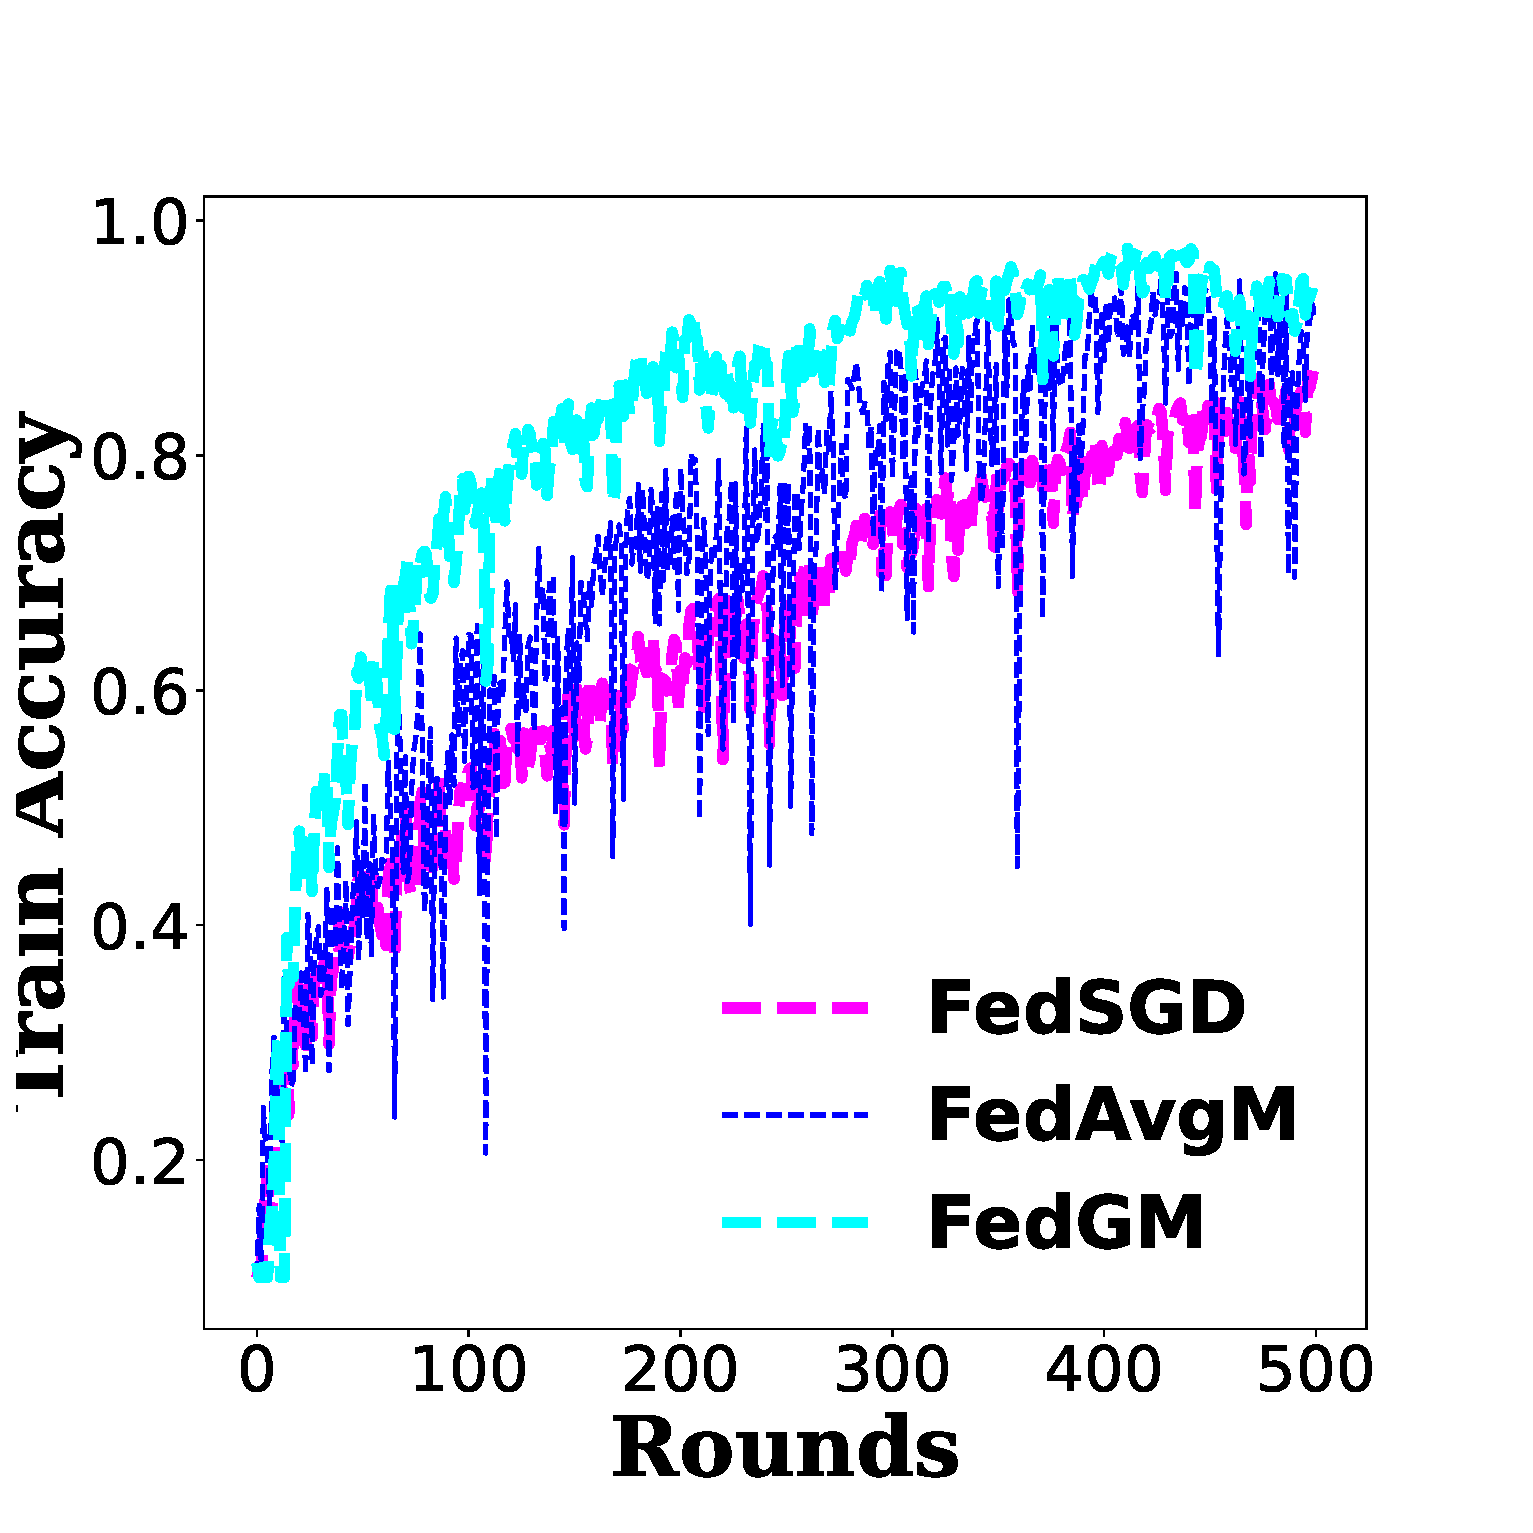
\includegraphics[width=.21\textwidth]{figs/resnet_cifar10_train.eps}
\label{subfig:resnet_cifar10_train}
}
\hspace{-2pt}
\subfigure{
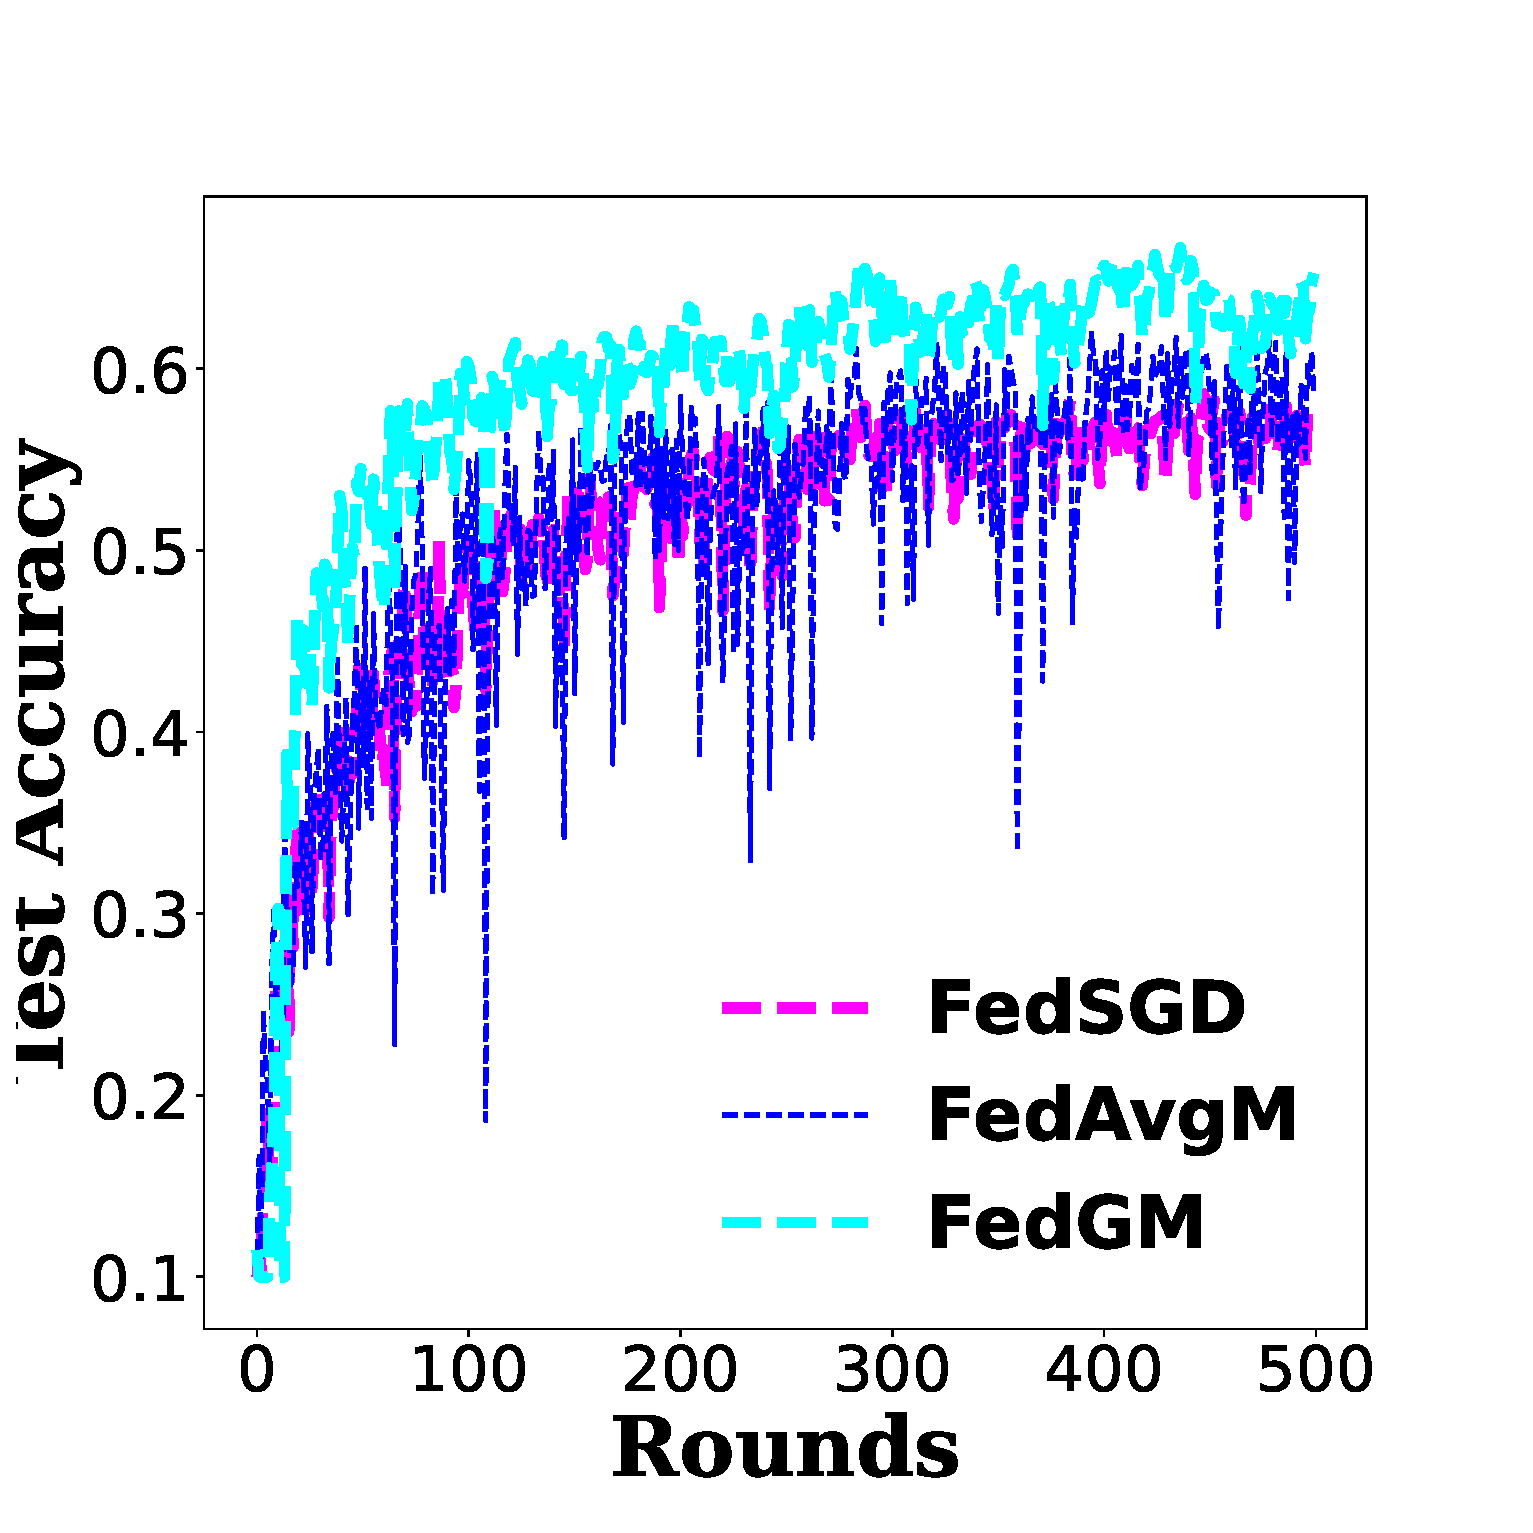
\includegraphics[width=.21\textwidth]{figs/resnet_cifar10_test.eps}
\label{subfig:resnet_cifar10_test}
}
\hspace{-2pt}
\subfigure{
\hspace{0pt}
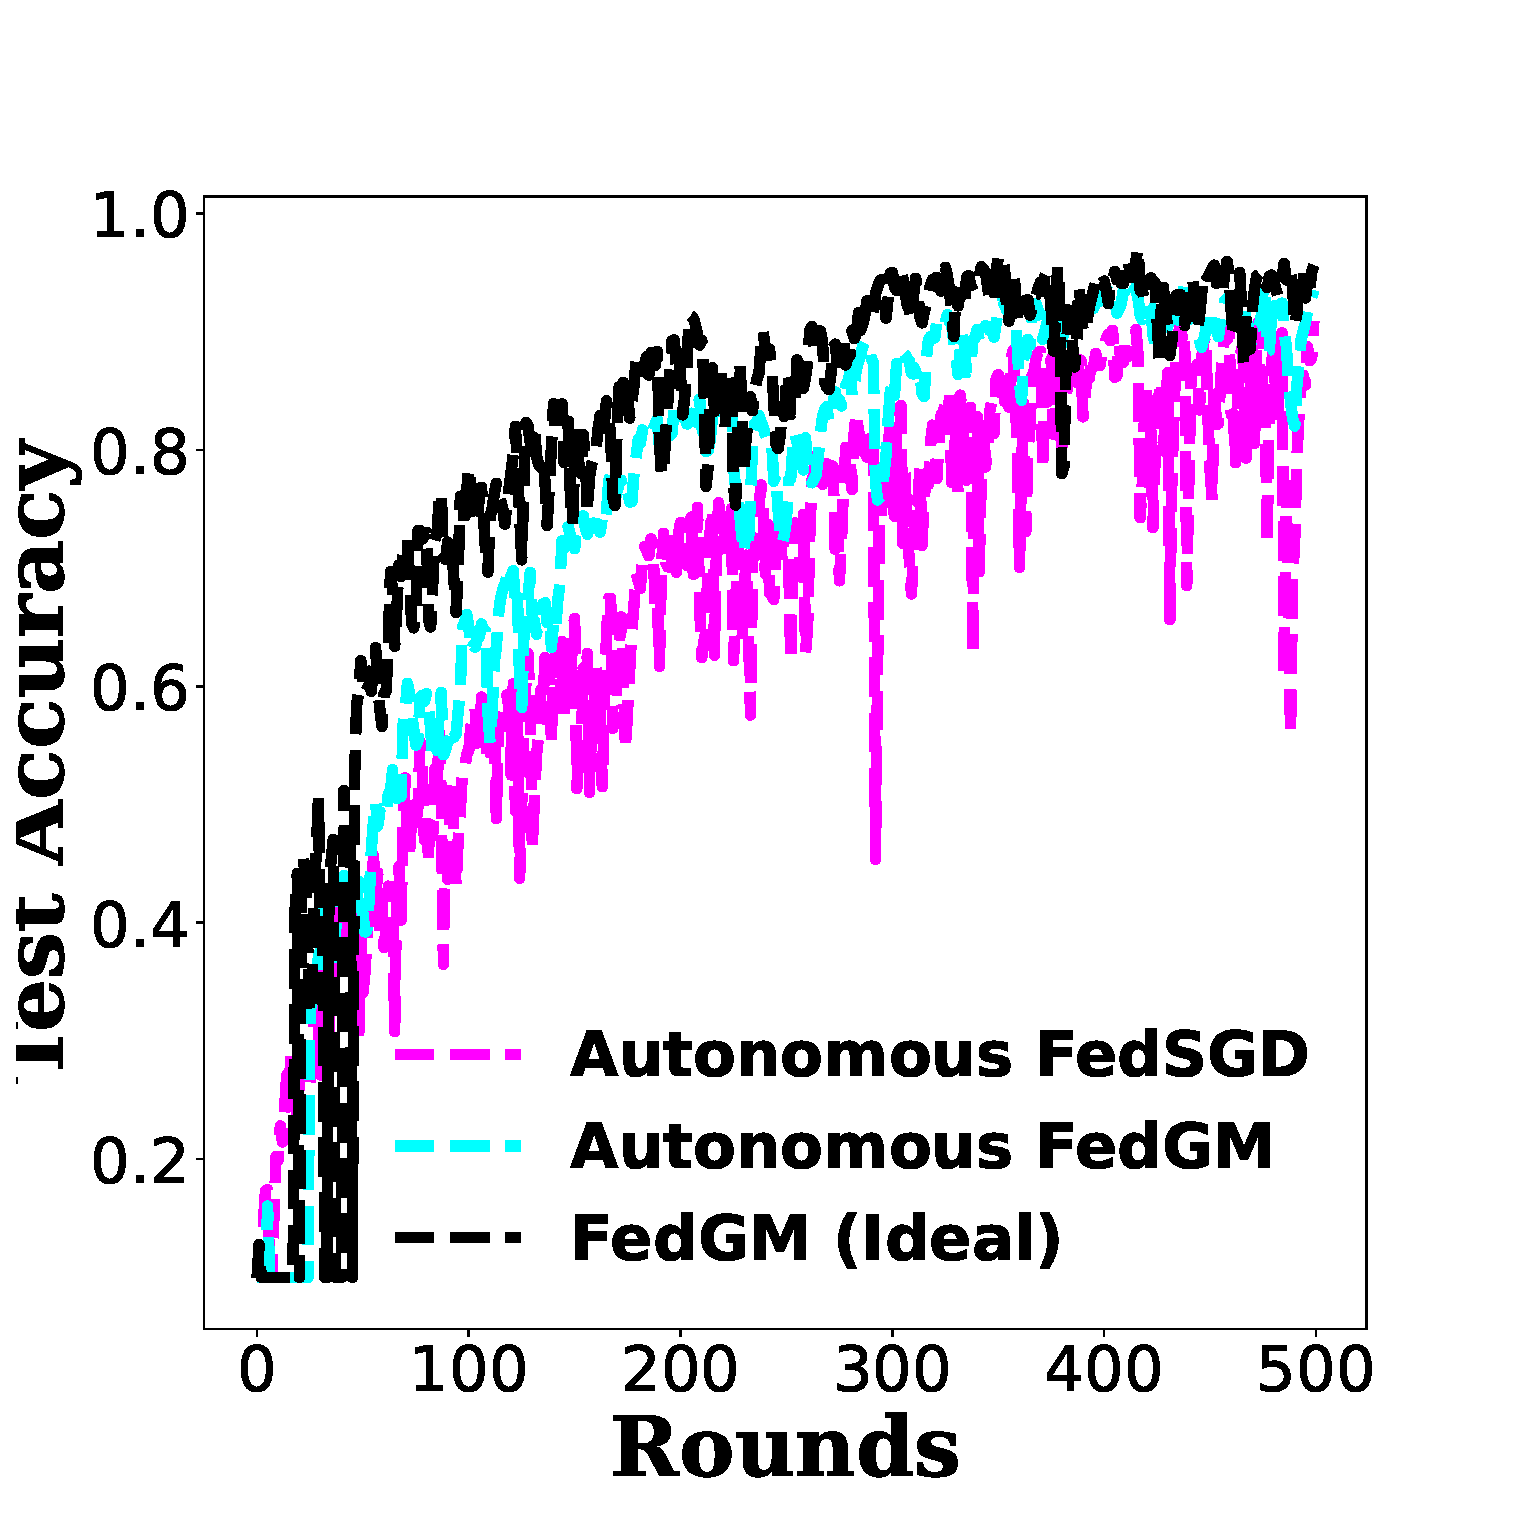
\includegraphics[width=.21\textwidth]{figs/autonomous_resnet_cifar10_train.eps}
\label{subfig:autonomous_resnet_cifar10_train}
}
\hspace{-2pt}
\subfigure{
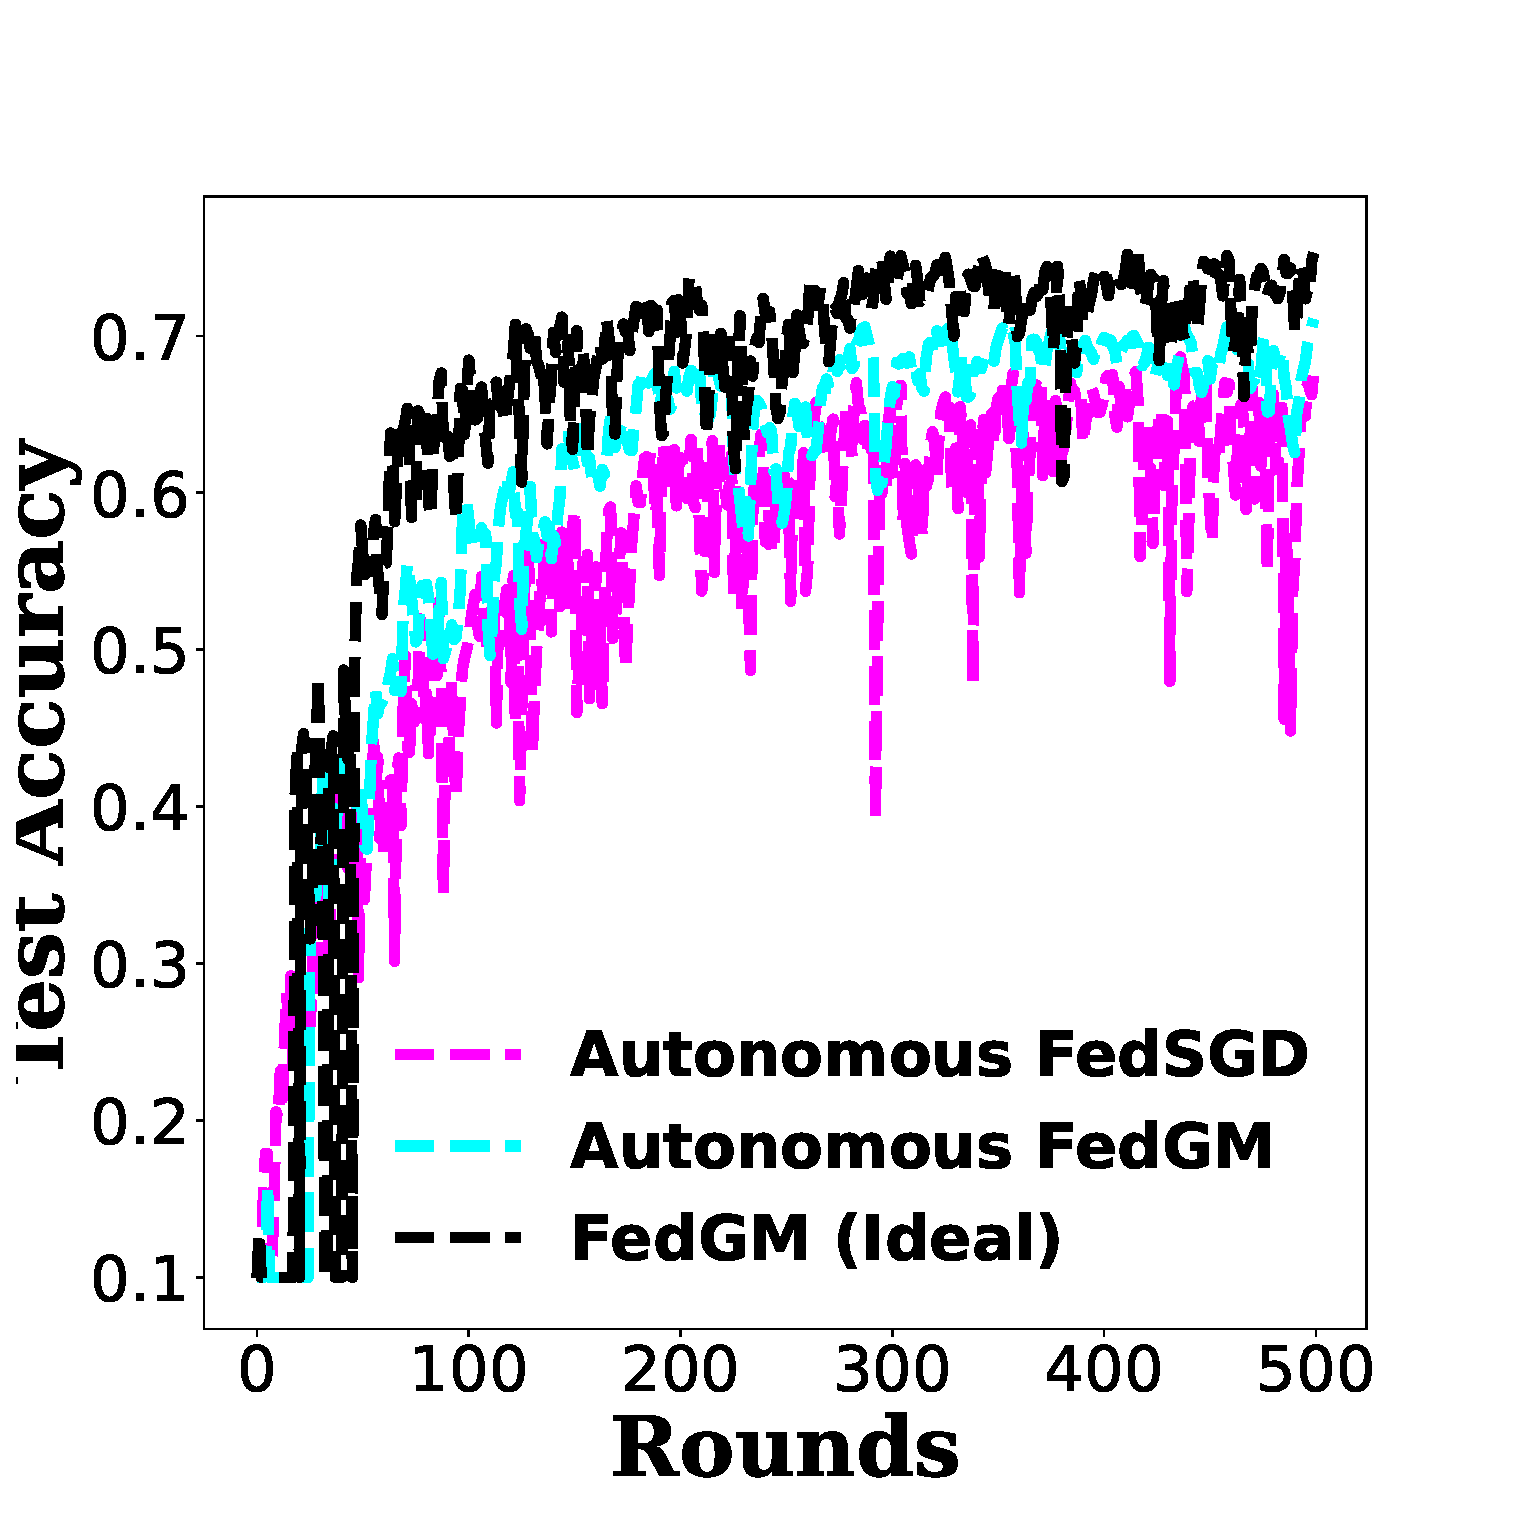
\includegraphics[width=.21\textwidth]{figs/autonomous_resnet_cifar10_test.eps}
\label{subfig:autonomous_resnet_cifar10_test}
}

\caption{\ref{subfig:resnet_cifar10_train} Training and \ref{subfig:resnet_cifar10_test} Testing Curves for FedGM (ResNet on CIFAR-10). FedGM outperforms FedAvg/FedAvgM. \ref{subfig:autonomous_resnet_cifar10_train} Training and \ref{subfig:autonomous_resnet_cifar10_test} Testing for Autonomous FedGM (ResNet on CIFAR-10).}
\label{fig:resnet_cifar10}

\end{figure}

\subsection{Convergence Analysis}

We state the convergence guarantee of autonomous multistage FedGM as follows,

\begin{theorem}
\label{multistage_fedgm_free_uniform_arrival_convergence_theorem}
We optimize $f(x)$ with Algorithm \ref{alg:autonomous_fedgm} under assumptions \ref{smoothness_assumption}-\ref{bounded_global_assumption}. Suppose the maximum delay is bounded, i.e. $\tau_{t,i}\leq\tau<\infty$ for any $i\in\mathcal{S}_t$ and $t\in\{0,1,\dots,T-1\}$. Under the condition $\eta_l\leq\min\left\{\frac{1}{8K_{t,\text{max}}L},\sqrt{\frac{1}{ 120L^2 C_\eta \tau K_{t,\text{max}}^2}} \right\}$, where $K_{t,\text{max}} =\max_{i\in\mathcal{S}_t}K_{t,i} $. And further assume each client is included in $\mathcal{S}_t$ with probability $\frac{m}{n}$ uniformly and independently. With necessary abbreviation for ease of notation \footnote{We denote $\Bar{\eta}\triangleq\frac{1}{S}\sum_{s=0}^{S-1}\eta_s$ (average server learning rate), $\hat{\eta}^2\triangleq\frac{1}{S}\sum_{s=0}^{S-1}\eta^2_s$, $\hat{\eta}^3\triangleq\frac{1}{S}\sum_{s=0}^{S-1}\eta^3_s$, $\frac{1}{K_t}=\frac{1}{m}\sum_{i\in\mathcal{S}_t}\frac{1}{K_{t,i}}$, $\bar{K}_t\triangleq \frac{1}{m}\sum_{i\in\mathcal{S}_t}K_{t,i}$, $\hat{K}_t^2 \triangleq \frac{1}{m}\sum_{i\in\mathcal{S}_t}K^2_{t,i}$, $\phi_1 \triangleq  \frac{1}{T}\sum_{t=0}^{T-1} \Bar{K}_t$, $\phi_2 \triangleq  \frac{1}{T}\sum_{t=0}^{T-1} \hat{K}_t^2$, and $\phi_3 \triangleq \frac{1}{T}\sum_{t=0}^{T-1} \frac{1}{K_t}$, for ease of notation.}, we would have:

\begin{gather*}
 \Bar{\mathcal{G}}
\leq \frac{4 \left(f(x_0) - f^\ast  \right)}{S W_2 \eta_l} 
+  \Phi_l \sigma_l^2
+ \Phi_g \sigma_g^2 
\label{multistage_fedgm_free_uniform_arrival_bound}
\end{gather*}
$\Phi_l \triangleq \frac{20  \eta^2_l L^2 T \Bar{\eta}}{W_2} \phi_1 + \frac{4 L^2\tau^2\hat{\eta}^3\eta_l^2T}{mW_2}\phi_3 + \frac{2 L^2W_1^2 \Bar{\eta} \eta_l T}{m W_2}\phi_3 + \frac{2 \Bar{\eta} \eta_l T}{m W_2}\phi_3 + \frac{2 L\hat{\eta}^2\eta_l}{m W_2}\phi_3$, and $\Phi_g \triangleq \frac{120 \eta^2_l L^2 T \Bar{\eta} \phi_2}{W_2}$. 
\end{theorem}



\begin{corollary}[Convergence Rate]
Suppose an identical $K$ for all $t$ and $i$. By appropriately setting $\Bar{\eta}$, $\eta_l$, $W_1$, $W_2$, we have the convergence rate as, $\mathcal{O}\left(\frac{1}{\sqrt{mKT}}\right)+ \mathcal{O}\left(\frac{\tau^2}{T}\right) +  \mathcal{O}\left( \frac{K^2}{T} \right)$.
\label{corollary:free_multistage_fedgm_rate}
\end{corollary}


\begin{remark}
Corollary \ref{corollary:free_multistage_fedgm_rate} indicates $\tau$ brings a slowdown in convergence. Fortunately, with a sufficiently large $T$ (e.g. $T\ge mK^5$) and a manageable $\tau$ (e.g. $\tau \leq \frac{T^\frac{1}{4}}{(mK)^\frac{1}{4}}$), autonomous multistage FedGM obtains a $\mathcal{O}\left(\frac{1}{\sqrt{mKT}}\right)$ rate. Note that we make an additional assumption that each client is included in $\mathcal{S}_t$ with probability $\frac{m}{n}$ uniformly and independently, which is necessary as the following Corollary \ref{corollary:free_multistage_fedgm_general_arrival_rate} indicates if without such assumption, the rate has a non-convergent $\mathcal{O}\left( \sigma_g^2 \right)$ term that we cannot avoid (the lower bound is $\Omega\left( \sigma_g^2 \right)$).
\end{remark}

\begin{corollary}[Convergence Rate w/o Uniform Sampling Assumption]
Suppose an identical $K$ for all $t$ and $i$. By appropriately setting $\Bar{\eta}$, $\eta_l$, $W_1$, $W_2$, we have the convergence rate as, $\mathcal{O}\left(\frac{1}{\sqrt{mKT}}\right)+ \mathcal{O}\left(\frac{\tau^2}{T}\right) +  \mathcal{O}\left( \frac{K^2}{T} \right) + \mathcal{O}\left( \sigma_g^2 \right)$, and the non-vanishing $\mathcal{O}\left( \sigma_g^2 \right)$ is unavoidable. \footnote{We informally state Corollary \ref{corollary:free_multistage_fedgm_general_arrival_rate} due to page limit, please refer to Appendix \ref{sec:proof_free_multistage_fedgm_general_arrival} for a formal statement.}
\label{corollary:free_multistage_fedgm_general_arrival_rate}
\end{corollary}





\section{Experimental Results}
\label{sec:experiments}

In this section, we present empirical evidence to verify our theoretical findings. We train ResNet \citep{He2016DeepResNet} and VGG \citep{Simonyan14VGG} on CIFAR10 \citep{Krizhevsky2009CIFAR}. To simulate data heterogeneity in CIFAR-10, we impose label imbalance across clients, i.e. each client is allocated a proportion of the samples of each label according to a Dirichlet distribution \citep{Hsu2019MeasuringTE, Yurochkin2019BayesianNF}. The concentration parameter $\alpha>0$ indicates the level of \textit{non-i.i.d.}, with smaller $\alpha$ implies higher heterogeneity, and $\alpha\to\infty$ implies \textit{i.i.d.} setting. Unless specified otherwise, we have 100 clients in all experiments, and the partial participation ratio is 0.05, i.e., 5 out of 100 clients are picked in each round, \textit{non-i.i.d.} is $\alpha=0.5$, and local epoch is 3. We defer many more results and details of hyperparameter settings to Appendix \ref{sec:appendix_exp}.

\subsection{Results on FedGM}
\label{subsec:exp_fedgm}

Figure \ref{fig:resnet_cifar10} shows the results for ResNet on CIFAR-10 with FedGM, FedAvgM, and FedAvg. We perform grid search over $\eta\in\{0.5,1.0,1.5,\dots,5.0\}$, $\beta\in\{0.7,0.9,0.95\}$, and $\nu\in\{0.7,0.9,0.95\}$. We report their respective best results in Figure \ref{fig:resnet_cifar10}. We observe that though FedAvgM converges faster than FedAvg, it is only marginally better in terms of testing. FedGM, in contrast, outperforms FedAvgM and FedAvg in both measures. Therefore, a general momentum, instead of only SHB, is critical empirically. We analyze possible reasons and leave more results with VGG and different heterogeneity levels $\alpha$ to Appendix \ref{subsec:appendix_more_results_fedgm}.

\iffalse

\begin{figure}[h]

\centering
\subfigure{
\hspace{0pt}
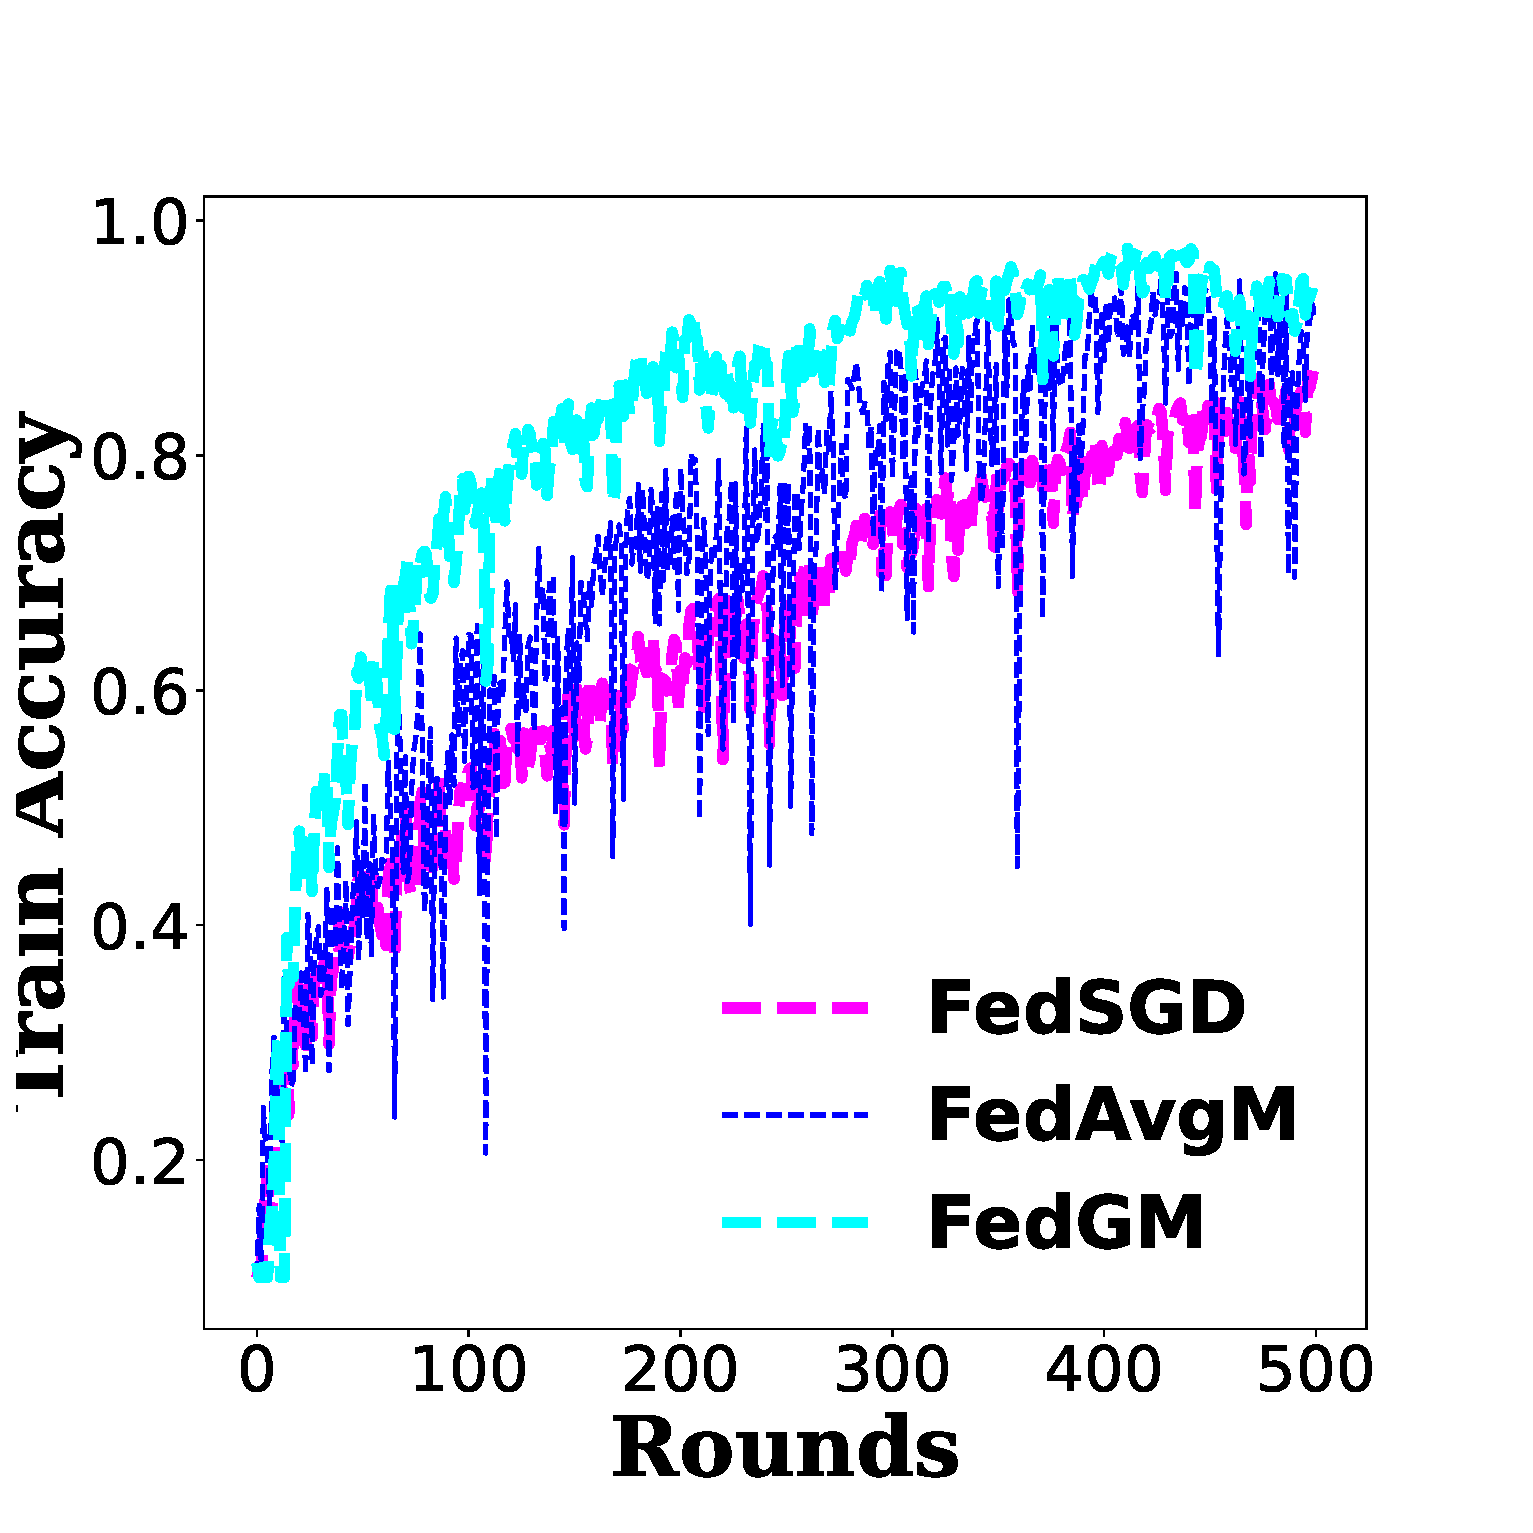
\includegraphics[width=.22\textwidth]{figs/resnet_cifar10_train.eps}
\label{subfig:resnet_cifar10_train}
}
\hspace{-6pt}
\subfigure{
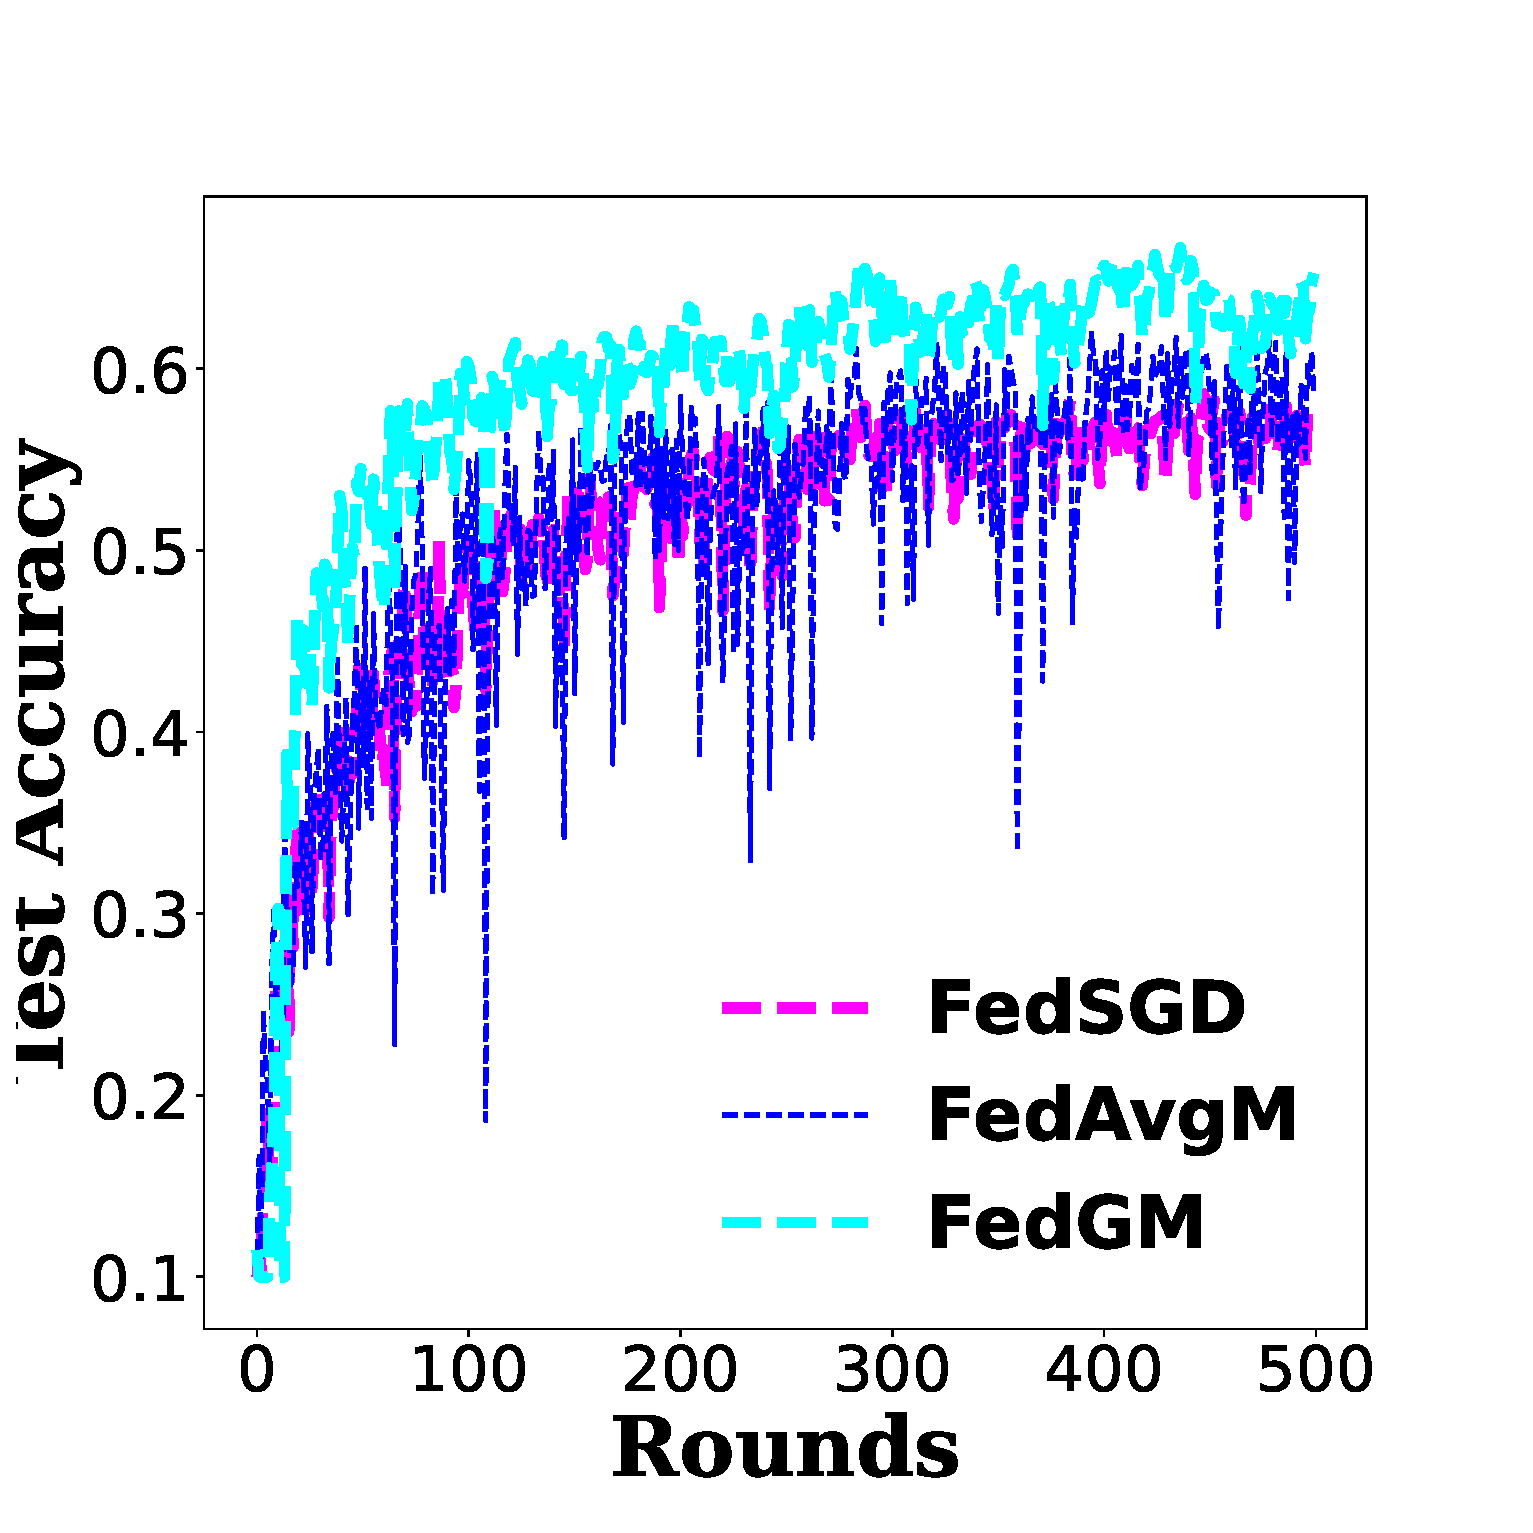
\includegraphics[width=.22\textwidth]{figs/resnet_cifar10_test.eps}
\label{subfig:resnet_cifar10_test}
}

\caption{\ref{subfig:resnet_cifar10_train} Training and \ref{subfig:resnet_cifar10_test} Testing Curves for ResNet on CIFAR-10. FedGM outperforms FedAvg/FedAvgM.}
\label{fig:resnet_cifar10}
\vspace*{-10pt}
\end{figure}

\subsection{Results on Multistage FedGM}
\label{subsec:exp_multistage_fedgm}

\fi




\subsection{Results on Multistage FedGM}
\label{subsec:exp_multistage_fedgm}


Figure \ref{fig:resnet_cifar10_multistage} shows the results for ResNet on CIFAR-10 with multistage vs. single-stage FedGM. The two black vertical lines at round 143 and 429 mark the end of 1st/2nd stage. For multistage FedGM, $(\eta_1=2.0,\eta_2=1.0,\eta_3=0.5)$, the $\beta$ also changes according to Eq. \ref{stagewise_hyper_constraints}. From Figure \ref{fig:resnet_cifar10_multistage}, we observe multistage FedGM is better than single-stage FedGM, no matter what constant $\eta$ it takes. Specifically, at first stage, $\eta_1=2.0$ makes the training curve fluctuate dramatically, but later into 2nd/3rd stage, the training stabilizes with smaller $\eta_2$ and $\eta_3$. Multistage FedGM achieves a balance between early exploration and late exploitation. Multistage is also superior to its counterpart in testing. We leave more experiments to Appendix \ref{subsec:more_exp_multistage_appendix}.

\begin{figure}[h]

\centering
\subfigure{
\hspace{0pt}
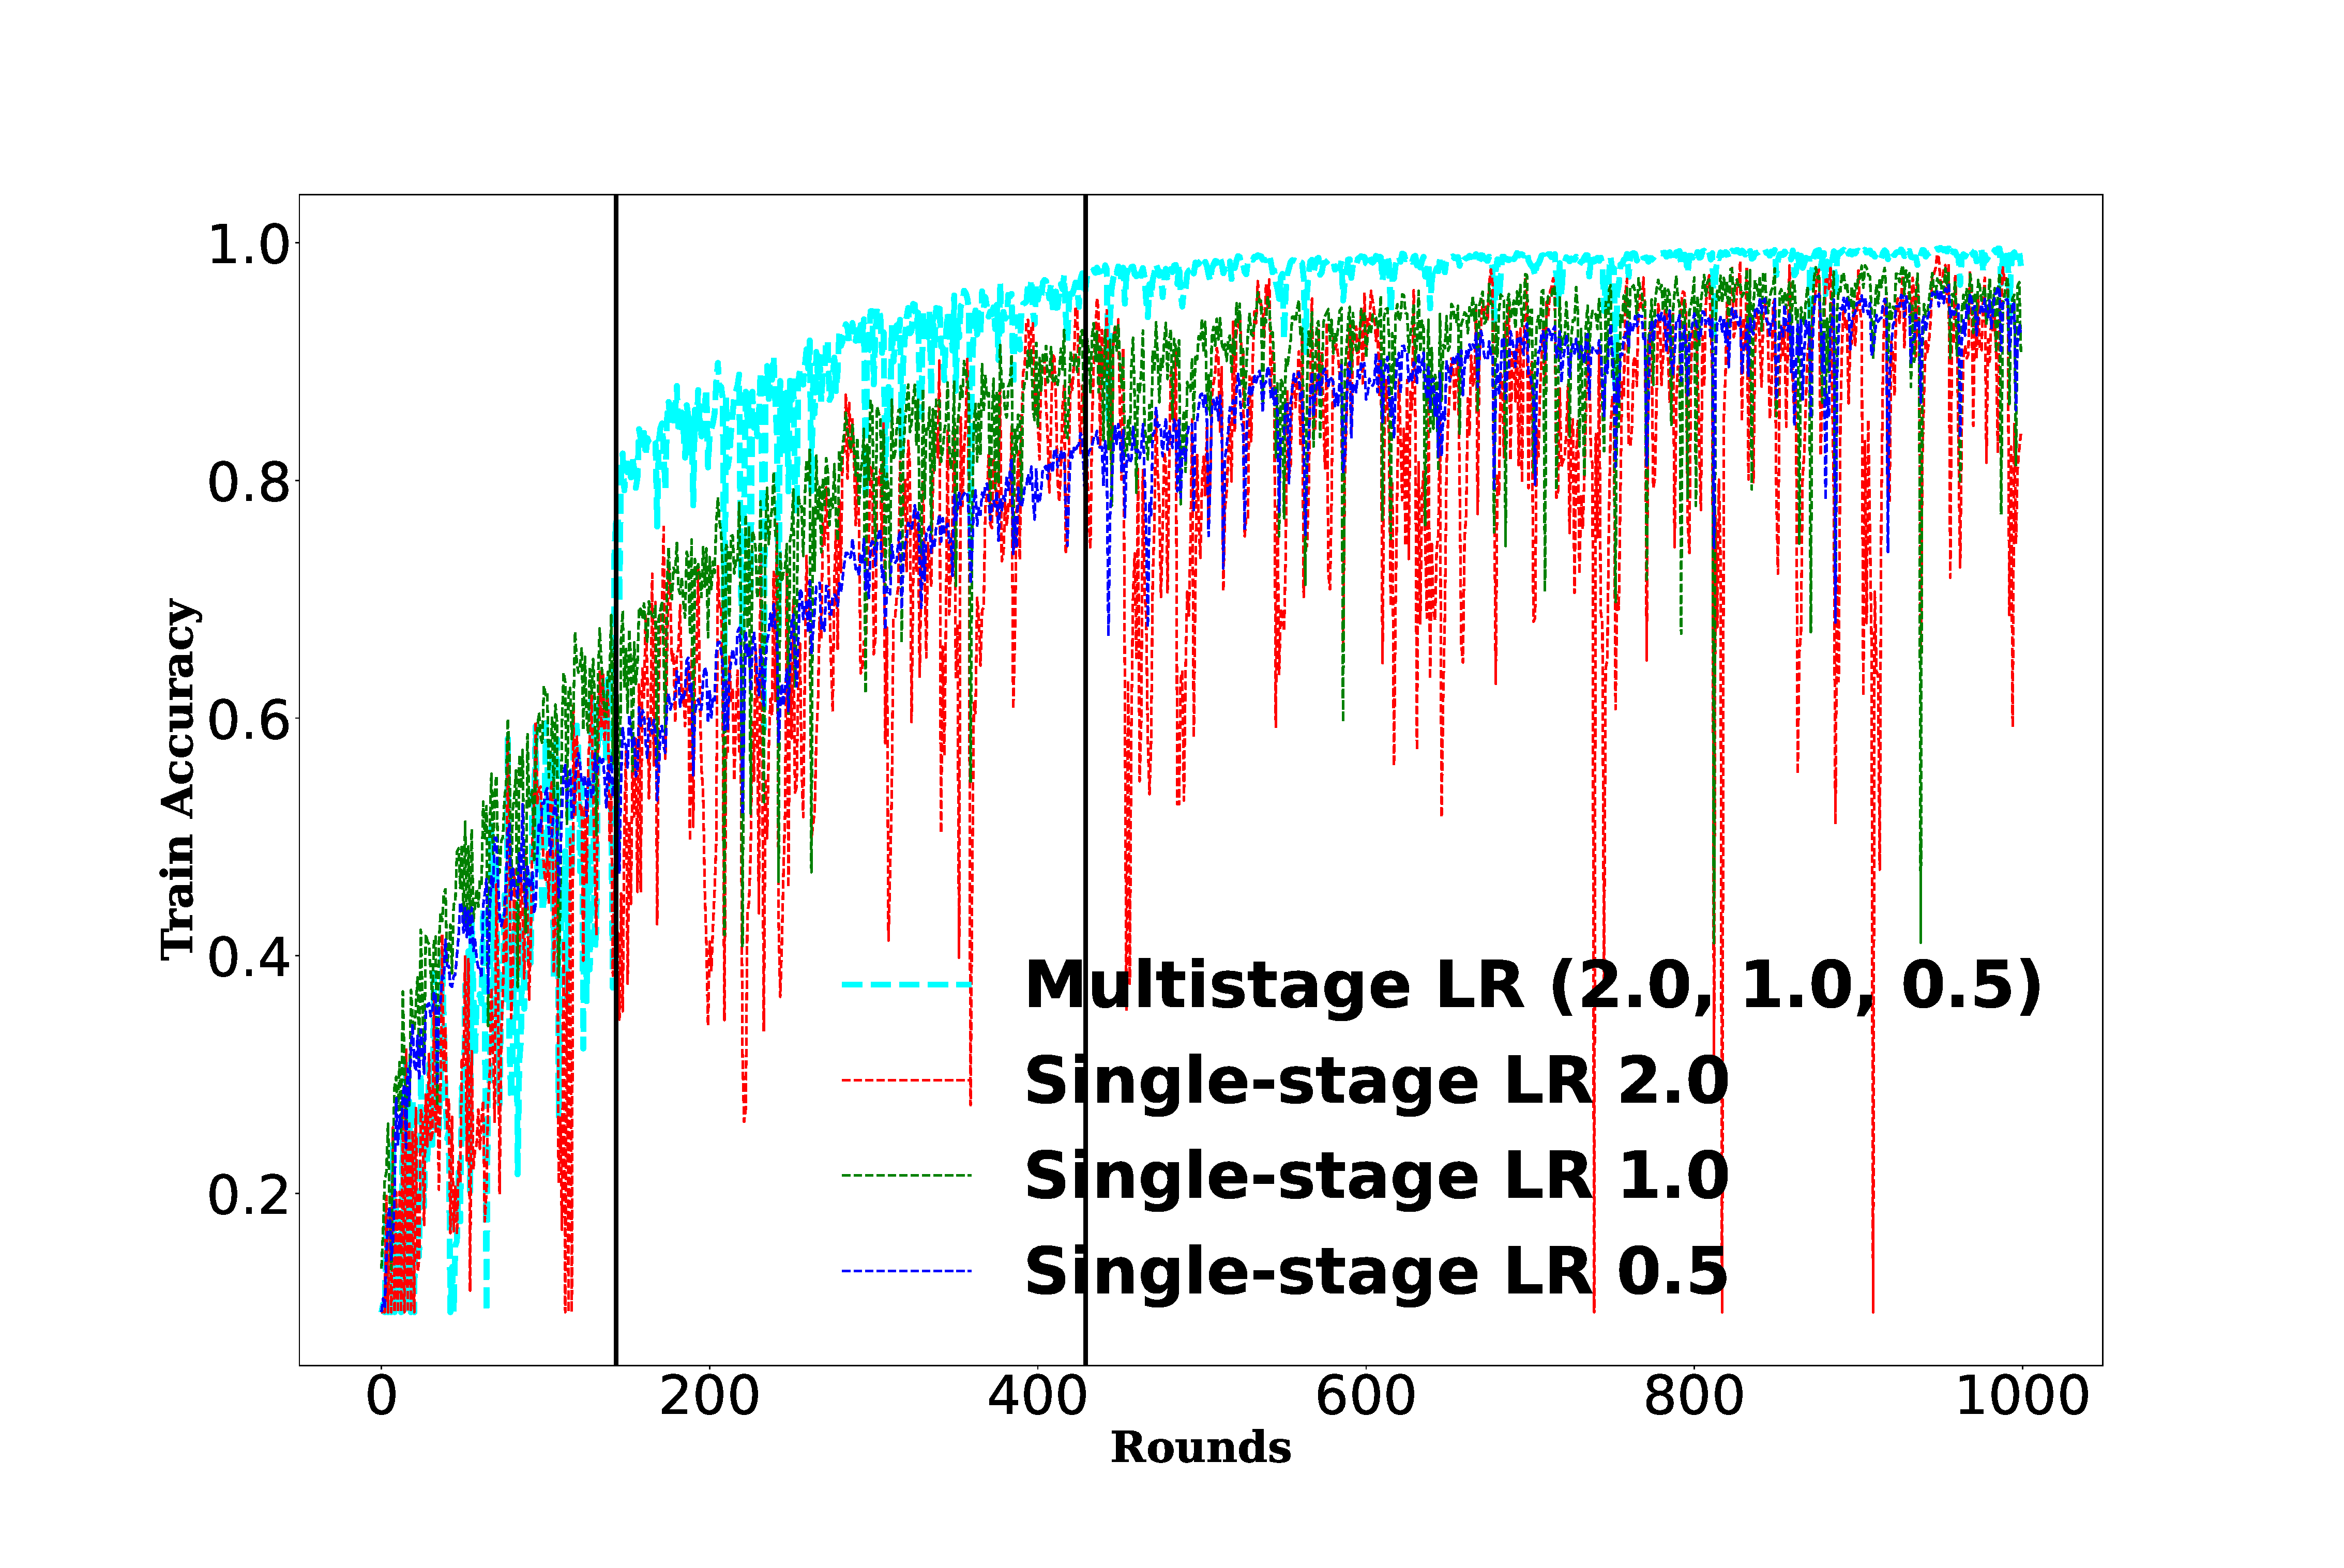
\includegraphics[width=.35\textwidth]{figs/multistage_train.eps}
\label{subfig:multistage_resnet_cifar10_train}
}
\subfigure{
\hspace{0pt}
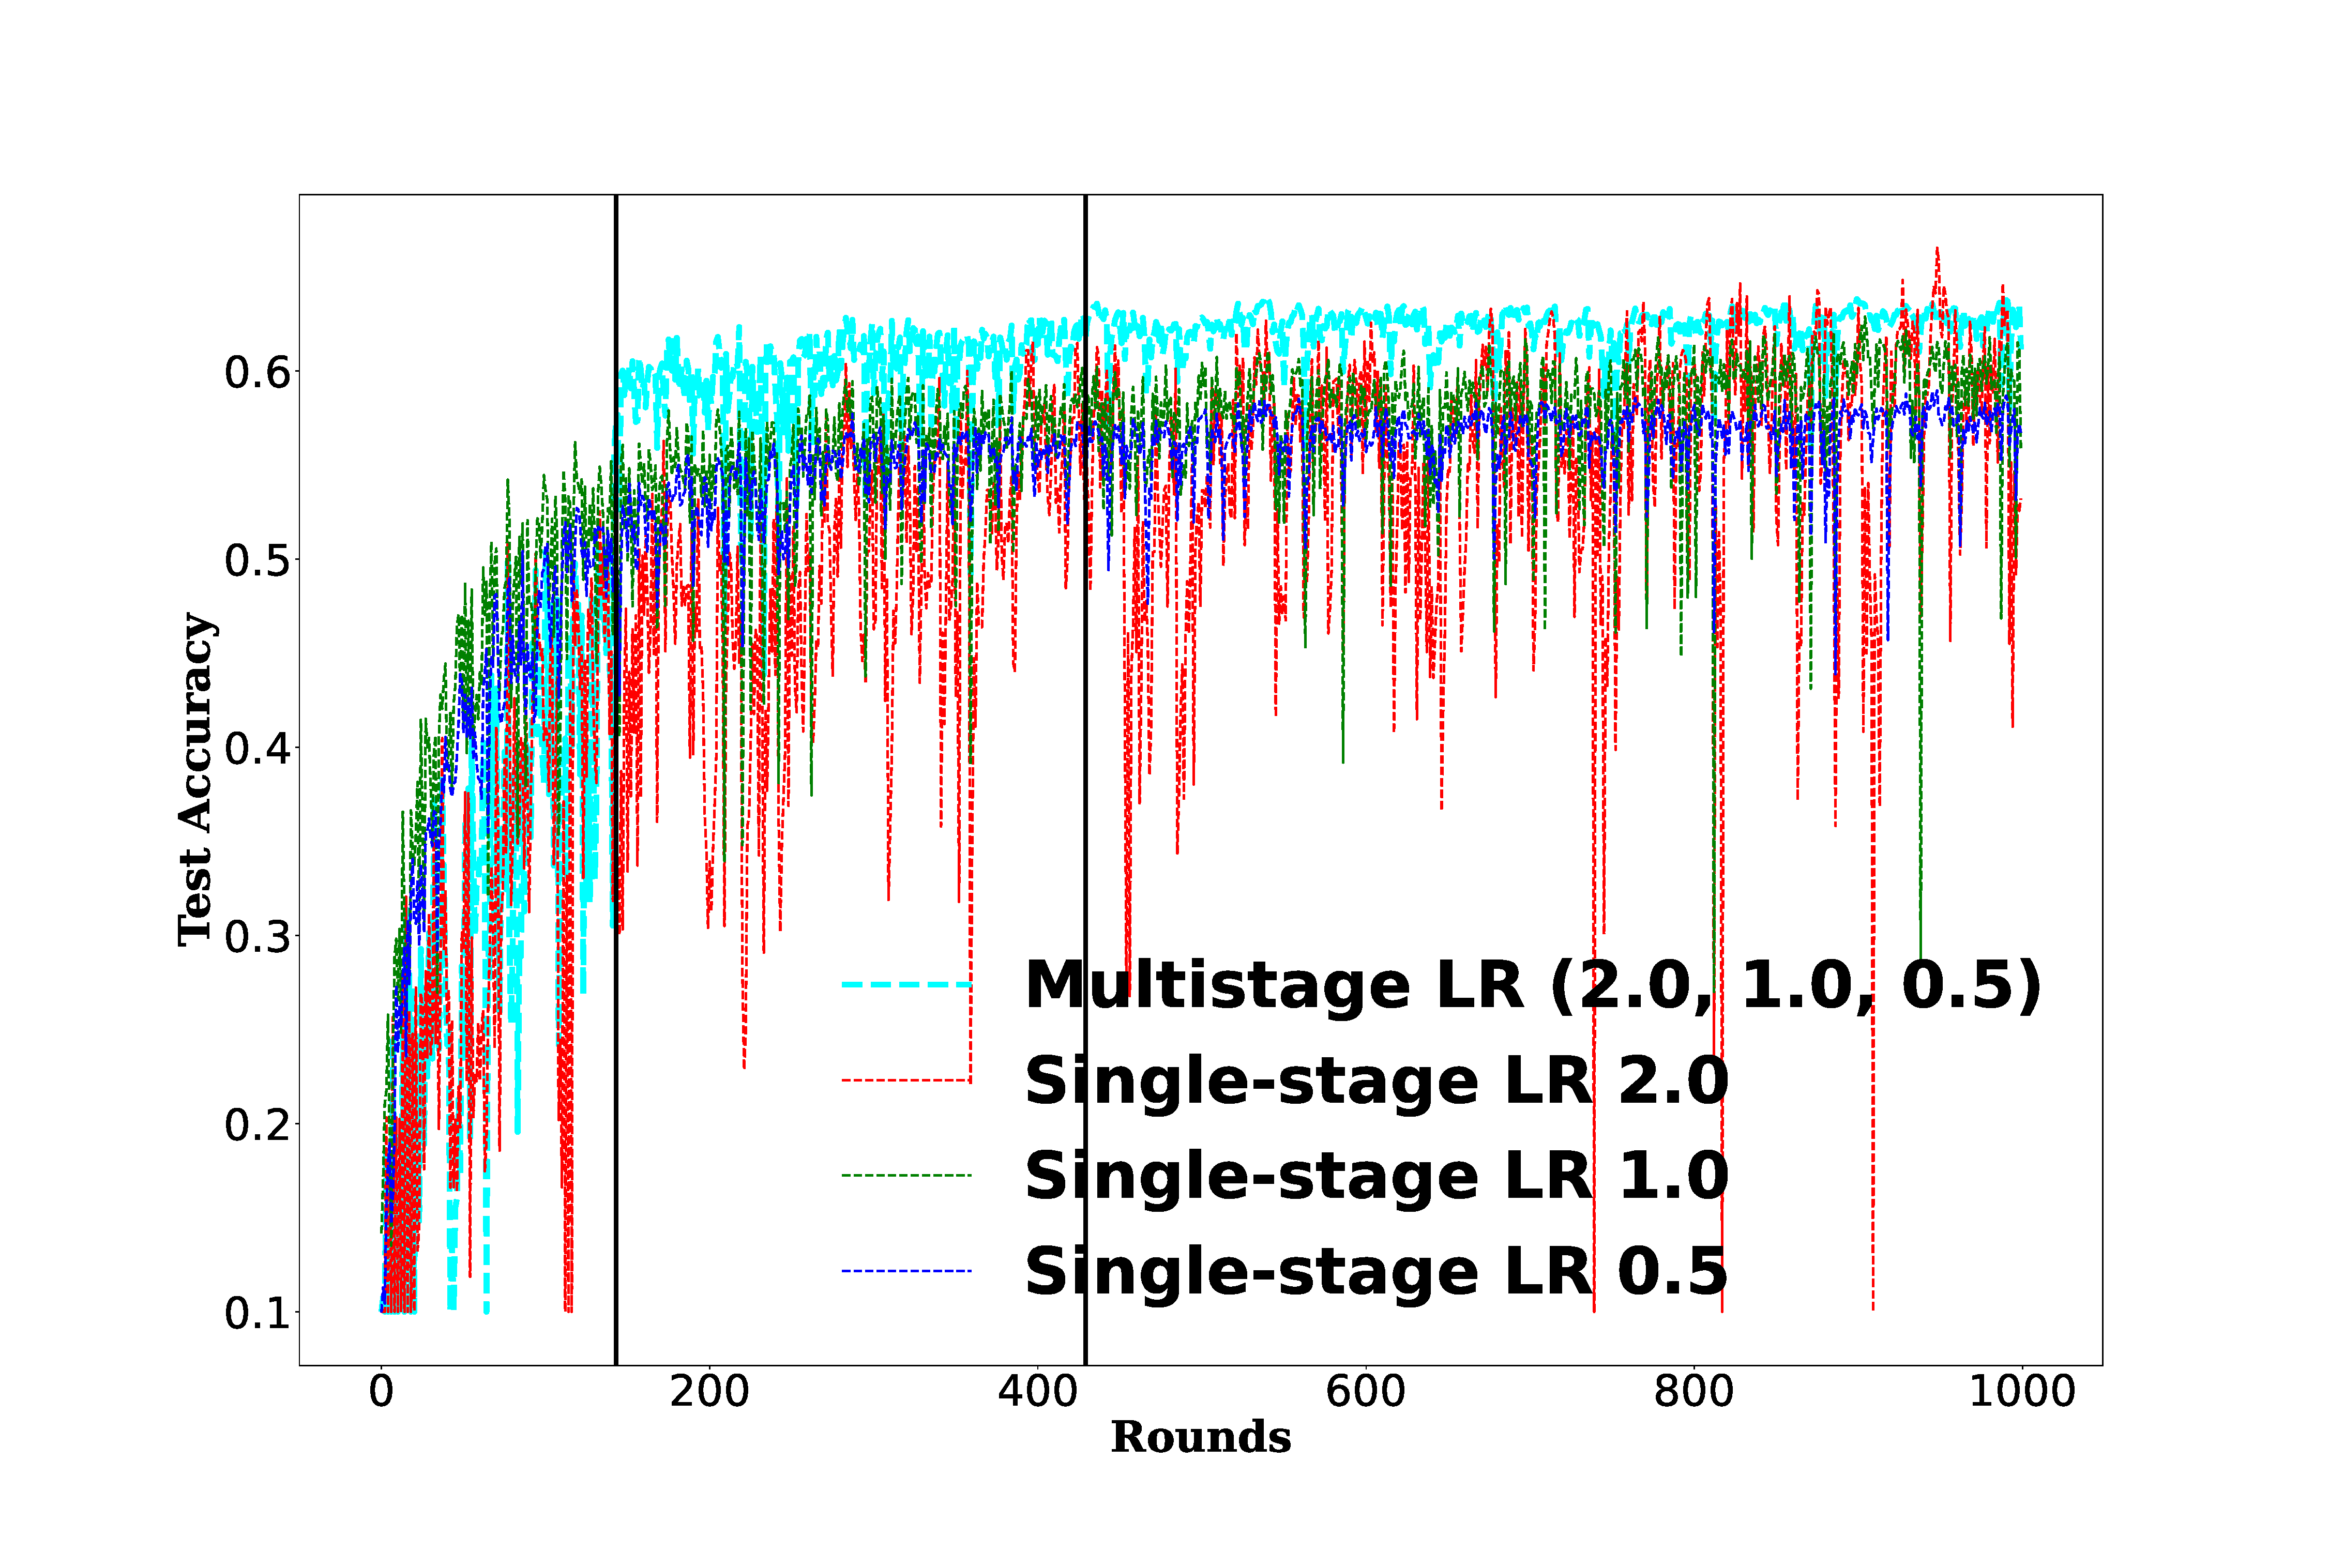
\includegraphics[width=.35\textwidth]{figs/multistage_test.eps}
\label{subfig:multistage_resnet_cifar10_test}
}

\caption{\ref{subfig:multistage_resnet_cifar10_train} Training and \ref{subfig:multistage_resnet_cifar10_test} Testing Curves for Multistage FedGM vs. Single-stage FedGM.}
\label{fig:resnet_cifar10_multistage}
\end{figure}




\subsection{Results on Autonomous FedGM}
\label{subsec:exp_autonomous_fedgm}

Figure \ref{fig:resnet_cifar10} shows the results for ResNet on CIFAR-10 with Autonomous FedGM (\& FedAvg). Please refer to Appendix \ref{subsec:exp_settings_appendix} for detailed settings. We perform a grid search as in Section \ref{subsec:exp_fedgm}. We report their respective best curves. We plot an ideal FedGM (i.e. synchronous and identical local epochs) as reference line. We could observe Autonomous FedGM outperforms Autonomous FedAvg with system heterogeneity. Though Autonomous FedGM suffers a slowdown compared to the ideal FedGM, it is within a small margin, which supports our theory in Corollary \ref{corollary:free_multistage_fedgm_rate} and validates the effectiveness of Autonomous FedGM. We leave more experiments to Appendix \ref{subsec:appendix_more_exp_autonomous}.







\section{Conclusion}
\label{sec:conclusion}

This paper systematically studied how the server momentum could help alleviate client drift that arises from both data heterogeneity and system heterogeneity. We demonstrated the critical role of momentum schemes and proper hyperparameter schedule by providing a rigorous convergence analysis and extensive empirical evidence, which pave a way for more widely and disciplined use of server momentum in the federated learning research community. 

\section{Acknowledgments}
This work was partially supported by NSF 2217071, 2213700, 2106913, 2008208, 1955151 at UVA.
This work was partially supported by NSF IIS 2347592, 2348169, 2348159, 2347604, CNS 2347617, CCF 2348306, DBI 2405416 at Pitt and UMD.


% \pagebreak
% \medskip

\newpage

\bibliography{jianhui}



\newpage
\onecolumn
\appendix
\centerline{\huge\textbf{Appendix}}

\section{Organization of Appendix}

Appendix is organized as follows. In Section \ref{sec:autonomous_multistage}, we discuss the omitted details of server momentum with system heterogeneity from Section \ref{sec:autonomous}. In Section \ref{sec:related_work}, we provide the discussion of related works. In Section \ref{sec:proof_multistage_fedgm_full_participation}, we show the proof of Theorem \ref{multistage_fedgm_full_participation_convergence_theorem}, Corollary \ref{corollary:multistage_fedavg_full_participation}, and Corollary \ref{corollary:multistage_fedgm_full_participation}. In Section \ref{sec:proof_multistage_fedgm_partial_participation}, We provide the proof of Theorem \ref{multistage_fedgm_partial_participation_convergence_theorem} and Corollary \ref{corollary:fedgm_partial_participation_convergence_rate}. In Section \ref{sec:proof_free_multistage_fedgm_uniform_arrival}, we provide the proof of Theorem \ref{multistage_fedgm_free_uniform_arrival_convergence_theorem} and Corollary \ref{corollary:free_multistage_fedgm_rate}. In Section \ref{sec:proof_free_multistage_fedgm_general_arrival}, we provide the proof of Corollary \ref{corollary:free_multistage_fedgm_general_arrival_rate}. Note that we use a 0-indexing for $T$ and $S$ in most proofs, i.e. the rounds (stages) are denoted as $\{0,\dots,T-1\}$ ($\{0,\dots,S-1\}$), which is equivalent to the 1-indexing in main text, i.e. $\{1,\dots,T\}$ ($\{1,\dots,S\}$). Finally, in Section \ref{sec:appendix_exp}, we provide experimental settings and extra experimental results that are omitted from main text.


\section{Autonomous Multistage FedGM}
\label{sec:autonomous_multistage}

In this section, we discuss the omitted details of server momentum with system heterogeneity from Section \ref{sec:autonomous}.

\subsection{Ubiquitous System Heterogeneity}

For a simplified abstraction of real world settings, most FL algorithms make the assumption that, all clients initialize with the same global model and they conduct identical number of local updates at any given round.

More formally, we could observe from LocalOPT (Algorithm \ref{alg:localopt}) that the following assumptions have been made, (a) \textit{Homogeneous Local Updates} all participating clients would do local gradient descent for $K$ steps; (b) \textit{Uniform Client Participation} each client would participate in a given communication round uniformly according to a given distribution that is independent across rounds; (c) \textit{Synchronous Local Clients} all participating clients always initialize at $x_t$, i.e., the global model at current timestamp. 



Though these three assumptions have been adopted in most existing works \citep{McMahan2017FedAvg,Hsu2019MeasuringTE,Li20FedProx,karimireddy2020scaffold,reddi2020adaptive,wang22adaptive, hu2023beyond}, each of these assumptions rarely holds in reality. Due to unavoidable \textbf{heterogeneous client capability}, and \textbf{unpredictable availability}, enforcing identical local epochs and synchrony would incur straggler effect and unnecessary energy waste \citep{Kairouz21AdvancesProblems}. Therefore, realistic FL system is more economical to allow different local epochs and \textbf{asynchronous aggregation}.


When studying client heterogeneity and the resulting client drift, most works focus explicitly on data heterogeneity \citep{Li2020Fed-Non-IID,yang2021achieving}, while ignoring the equally ubiquitous system heterogeneity, which casts doubt on the applicability of the corresponding algorithms in practice.

\iffalse


\begin{algorithm2e}[tb]
\SetAlgoVlined
\KwIn{Same as Algorithm \ref{multistage_FedGM_algorithm}}
\SetAlgoLined
\For{$s\in\{1,...,S\}$}
{
\For{$t $ \text{in stage} $s$}
{   
    \colorbox{babyblueeyes}{\textbf{At Each Client (Concurrently)}}
    
    Once decided to participate in the training, retrieve $x_\mu$ from the server and its timestamp, set $x_{\mu,0}^i=x_\mu$.

    Select a number of local steps $K_{t,i}$, which is time-varying and device-dependent.

    $\Delta_\mu^i=\textbf{LocalOPT}\left(i,\eta_l,K_{t,i},x_\mu\right)$

    Normalize and send $\Delta_\mu^i=\frac{\Delta_\mu^i}{K_{t,i}}$
    

    \colorbox{babyblueeyes}{\textbf{At Server (Concurrently)}}
    
    Collect $m$ local updates $\{\Delta_{t-\tau_{t,i}}^i, i\in\mathcal{S}_t\}$ returned from the clients to form set $\mathcal{S}_t$, where $\tau_{t,i}$ is the random delay of the client $i$'s local update, $i\in\mathcal{S}_t$

    Aggregate $\Delta_t=\frac{1}{\lvert\mathcal{S}_t\rvert}\sum_{i\in \mathcal{S}_t}\Delta_{t-\tau_{t,i}}^i$

    $d_{t+1}=(1-\beta_s)\Delta_{t}+\beta_s d_{t}$

    $h_{t+1}=(1-\nu_s)\Delta_{t}+\nu_s d_{t+1}$
        
    Update $x_{t+1}=x_t-\eta_s h_{t+1}$

}
}
return $x_T$
\caption{\colorbox{babyblueeyes}{Autonomous Multistage FedGM}}
\label{alg:autonomous_fedgm}
\end{algorithm2e}

\fi

\subsection{Autonomous Multistage FedGM}

In light of the limitations of existing works, we aim to propose a general framework that enables all three features, i.e. \textbf{heterogeneous local computing}, \textbf{asynchronous aggregation}, and \textbf{flexible client participation}, which is formalized in Algorithm \ref{alg:autonomous_fedgm}.

Specifically, in Autonomous Multistage FedGM, the client decides when to participate in the training, and idling between rounds or even completely unavailable are both allowed. Once it decides to participate at round $t$, it retrieves current global model $x_\mu$ from the server and initializes $x_{\mu,0}^i=x_\mu$ locally, and conduct $K_{t,i}$ local steps to update from $x_{\mu,0}^i$ to $x^i_{\mu,K_{t,i}}$. Note in vanilla FedAvg, $K_{t,i}=K$ for any $i$ and $t$. In contrast, we allow $K_{t,i}$ to be time-varying and device-dependent. The client then normalizes the model update by $K_{t,i}$, i.e. $\Delta_\mu^i=\frac{x_{\mu,0}^i-x_{\mu,K_{t,i}}^i}{K_{t,i}}$, to avoid model biased towards clients with more local updates. Concurrently, the server collects the model updates from the clients. As every client may participate in training at a different round, the collected model update $\Delta_{t-\tau_{t,i}}^i$ may be from a historic timestamp, i.e. $\tau_{t,i}$ away from current time $t$. If we set the random delay $\tau_{t,i}=0$, it would be ordinary synchronous aggregation. The server triggers global update whenever it collects $m$ model updates and we denote the set of $m$ responsive clients as $\mathcal{S}_t$. The global update is same as multistage FedGM (i.e. Lines 11-13). Note that server optimization is concurrent with clients, i.e., the global update happens whenever $m$ model updates are collected, regardless of whether there are still some clients conducting local computation, thus ensuring there is no straggler.


Autonomous multistage FedGM will recover multistage FedGM, i.e. Algorithm \ref{multistage_FedGM_algorithm}, if we set $K_{t,i}=K$ and $\tau_{t,i}=0$ for $\forall t, i$. Please note that varying $K_{t,i}$ and nonzero $\tau_{t,i}$ bring nontrivial extra complexity to the theoretical analysis as can be seen in our proof.


\section{Related Work}
\label{sec:related_work}

\subsection{Tackling Client Heterogeneity and Client Drift in FedAvg}
\label{subsec:fedavg_related_work}

Deep learning models have been widely applied in many different domains, e.g. \cite{Mnih2013PlayingAW,He2016DeepResNet,Devlin2019BERT,Jure2017GNN,google16deep&wide,SuoICHI19,Xun2020CorrelationNF,Wu2023DiPmarkAS}, mostly in centralized environment. Due to privacy concerns and regulatory requirements \cite{european_commission_regulation_2016,California_Consumer_Privacy_Act_CCPA}, Federated Averaging (FedAvg) \cite{McMahan2017FedAvg} has been applied to avoid data transmission in collaborative training of deep learning models in a wide range of settings \cite{Li20FedProx,rothchild20fetchsgd,Wang20FedNova,fallah2020personalized,li2021model,bao2023adaptive,wu2023federated,wu2023solving}.

Client heterogeneity and its resulting client drift is known to destabilize FedAvg convergence \citep{zhao2018federated-noniid,karimireddy2020scaffold}. FedProx \citep{Li20FedProx} proposes to regularize the difference against global model in local objective. SCAFFOLD \citep{karimireddy2020scaffold} leverages variance reduction technique to reduce client drift and achieves the best known $\mathcal{O}\left(\frac{1}{\sqrt{nKT}}\right)$ rate in full participation setting. However, SCAFFOLD is not stateless which restricts its application in cross-device FL. \cite{reddi2020adaptive,wang22adaptive} propose a family of federated adaptive optimizers e.g. FedADAM, FedADAGRAD, and FedAMS that are natural extensions from non-FL adaptive optimizers to FL settings. Recent works propose algorithms to alleviate client heterogeneity in FL bilevel optimization problems, e.g. minimax \cite{wu2023solving} or conditional stochastic optimization \cite{wu2023federated}. The most relevant line of research to this paper is on server-side momentum. Server-side momentum is first empirically studied in \citep{Hsu2019MeasuringTE}, where FedAvgM is observed to outperform FedAvg in \textit{non-i.i.d.} settings by a significant margin. Recent explorations include \citep{rothchild20fetchsgd} that studies the interplay between server momentum and compression, and \citep{khanduri2021stem} which studies a two-sided momentum scheme that allows both server momentum and client momentum. However, all existing works have the following limitations that our paper aims to address, (a) they do not provide a unified analysis for a family of momentum schemes; (b) they do not incorporate any realistic hyperparameter schedulers; (c) they ignore an important source of client heterogeneity, i.e. system heterogeneity.


\subsection{Hyperparameter Scheduling}
\label{subsec:multistage_related_work}


Adaptively adjusting hyperparameters throughout the training is key to the success of deep model training, but most of such explorations are in non-FL context. For example, previous works \cite{He19ControlBatch}, \cite{Sun22Hyperparameters}, and \cite{Sun23Diffusion} reveal the connection between hyperparameters and generalization capacity of optimizers. \cite{Krizhevsky12ImageNet} and \cite{He16Res} propose to decay learning rate $\eta$ whenever the loss saturates; \cite{GoyalDGNWKTJH17LargeMinibatch} popularizes the heuristic of warmup to increase $\eta$ from a small value to a very large value in the first few iterations; \cite{Smith17Cyclic} proposes to adopt a cyclic learning rate schedule between warmup and decay phases. Apart from learning rate, adaptively scheduling other hyperparameters (e.g. momentum factor and batch size) is also shown to be very effective in many settings. For example, \cite{Sutskever13Init} shows a slowly increasing schedule for the momentum factor is crucial; \cite{Smith18Bayesian,Smith18DontDecay} propose a procedure to enable large batch training where $\eta$ and momentum factor $\beta$ are increasing, and batch size $B$ is scaled $B \propto \frac{\eta}{1-\beta}$. From a theoretical point of view, in non-FL context, \cite{Ge2019TheSD} and \cite{wang21stepdecay} show the multistage learning rate scheduler achieves a near-optimal convergence rate of $\mathcal{O}\left(\frac{\log T}{T}\right)$ rate (faster than polynomial decay), in both convex and non-convex functions. \cite{sun21stagewise} and \cite{Sun23TKDD} show the convergence of multistage scheduler for momentum schemes. However, to our best knowledge, there is no prior work studying multistage hyperparameter scheduler (both learning rate and momentum factor) in FL settings.

\subsection{Flexible Participation and Asynchronous Aggregation}
\label{subsec:asyn_aggregation_related_work}

The existing works that are dedicated to studying system heterogeneity can be mainly categorized into the following groups,

\iffalse

\begin{itemize}[leftmargin=*]
    \item Heterogeneous local computing but synchronous aggregation. \cite{Wang20FedNova} is probably the first work to show heterogeneous number of local updates results in the global model converges to a mismatched optimum which can be arbitrarily away from the true optimum and proposes an effective remedy FedNova to correct the mismatch. \cite{Basu19Qsparse-Local-SGD} considers how model compression works with different number of local updates \footnote{Though the authors call the proposed model 'asynchronous', the asynchrony refers to that updates occur after different number of local iterations but the local iterations are synchronous with respect to the global clock. However, 'asynchronous' in our context refers to local iterations are asynchronous with respect to the global clock, which is more challenging to analyze.}. \cite{Avdiukhin21arbitrarycommunication} focuses on a similar setting and studies the upper bound of distances between two consecutive communications to reduce communication times as much as possible. Their theoretical analysis relies on bounded gradient assumption.
    \item Flexible participation scheme but synchronous aggregation. There are mainly two line of works in this class. The first line focuses on the issue of intermittent client availability, FedLaAvg \cite{Yan2020DistributedClient} and MIFA \cite{gu2021arbitraryunavailable} both allow clients to participate arbitrarily. However, the proposed approach still requires all devices to respond at least in the first round. Moreover, the theoretical analysis of FedLaAvg requires bounded gradient assumption while MIFA requires a Lipschitz Hessian assumption, which are too stringent and unnecessary. \cite{wang2022arbitraryparticipation} systematically studies various participation patterns and which one of them guarantees convergences and whether the rate of convergence matches idealized participation scheme. However, their work considers synchronous aggregation and only the case of vanilla FedAvg. The second line concentrates on biased client selection \citep{Nishio2018ClientSelection, Chen2020ClientSampling, cho22biased_selection}. Most works study the biased sampling strategy in which the probability a client is sampled is related to its local loss to accelerate training \citep{Goetz2019ActiveFL,Ribero2020clientsampling}, which is inspired by similar strategy in centric computing \citep{Salehi2017BanditSampling,Jiang2019Local_Loss,shah20local_loss,Katharopoulos2018ImportanceSampling}. This line of works is less related to our proposed research.
    \item Asynchronous aggregation. This line of research is most closely related to our proposed Autonomous Multistage FedGM. However, though asynchrony has been a decade-long topic in traditional distributed computing \citep{Zhang2014DeepElasticAvg,Lian15Asynchronous,Zheng17ASGD}, it has received very limited attention in federated learning. \cite{Xie2019AsynchronousFO} proposes FedAsync in which the server immediately updates the global model whenever it receives a single local model. Their theoretical analysis only applies to convex objective function which is not applicable to deep learning. Moreover, this proposal has negative implication in privacy, as it no longer hides one single update in an aggregate, which is one of the most important points to use FL in the first place. In light of this, \cite{Nguyen2021FedBuff} proposes FedBuff, in which a global update is triggered when the server receives $m$ local updates, where $m$ is a pre-specified hyperparameter. By maintaining a size $m$ buffer, FedBuff could secure the identity of each local update and is empirically faster than FedAsync. However, it does not consider the heterogeneous local computing and does not provide a convergence rate that shows the dependency on $m$. \cite{Yang2021AnarchicFL} proposes anarchic FL in which the clients are free to determine how much local computation to conduct and the asynchronous communication is in the same fashion as FedBuff. However, \cite{Yang2021AnarchicFL} only considers the case of vanilla FedAvg, while our works subsumes anarchic FL as a special case.
\end{itemize}

\fi

\begin{itemize}[leftmargin=*]
    \item Heterogeneous local computing but synchronous aggregation. \cite{Wang20FedNova} is probably the first work to show heterogeneous number of local updates results in the global model converges to a mismatched optimum which can be arbitrarily away from the true optimum and proposes an effective remedy FedNova to correct the mismatch. \cite{Basu19Qsparse-Local-SGD} considers how model compression works with different number of local updates \footnote{Though the authors call the proposed model 'asynchronous', the asynchrony refers to that updates occur after different number of local iterations but the local iterations are synchronous with respect to the global clock. However, 'asynchronous' in our context refers to local iterations are asynchronous with respect to the global clock, which is more challenging to analyze.}. \cite{Avdiukhin21arbitrarycommunication} focuses on a similar setting and studies the upper bound of distances between two consecutive communications to reduce communication times as much as possible. Their theoretical analysis relies on bounded gradient assumption.
    \item Asynchronous aggregation. This line of research is most closely related to our proposed Autonomous Multistage FedGM. However, though asynchrony has been a decade-long topic in traditional distributed computing \citep{Zhang2014DeepElasticAvg,Lian15Asynchronous,Zheng17ASGD}, it has received very limited attention in federated learning. \cite{Xie2019AsynchronousFO} proposes FedAsync in which the server immediately updates the global model whenever it receives a single local model. Their theoretical analysis only applies to convex objective function which is not applicable to deep learning. Moreover, this proposal has negative implication in privacy, as it no longer hides one single update in an aggregate, which is one of the most important points to use FL in the first place. In light of this, \cite{Nguyen2021FedBuff} proposes FedBuff, in which a global update is triggered when the server receives $m$ local updates, where $m$ is a pre-specified hyperparameter. By maintaining a size $m$ buffer, FedBuff could secure the identity of each local update and is empirically faster than FedAsync. However, it does not consider the heterogeneous local computing and does not provide a convergence rate that shows the dependency on $m$. \cite{Yang2021AnarchicFL} proposes anarchic FL in which the clients are free to determine how much local computation to conduct and the asynchronous communication is in the same fashion as FedBuff. However, \cite{Yang2021AnarchicFL} only considers the case of vanilla FedAvg, while our works subsumes anarchic FL as a special case.
\end{itemize}

There are many other works that enable flexible participation scheme but still synchronous aggregation, e.g. \citep{Yan2020DistributedClient, gu2021arbitraryunavailable,wang2022arbitraryparticipation, Nishio2018ClientSelection, Chen2020ClientSampling, cho22biased_selection, Goetz2019ActiveFL,Ribero2020clientsampling}. This line of research is less related to our proposed research. 



\section{Proof of Theorem \ref{multistage_fedgm_full_participation_convergence_theorem}, Corollary \ref{corollary:multistage_fedavg_full_participation}, and Corollary \ref{corollary:multistage_fedgm_full_participation}}
\label{sec:proof_multistage_fedgm_full_participation}

\begin{proof}[Proof of Multistage FedGM with Full Participation]

Recall the formulation of General Momentum:
\begin{equation}
    \begin{gathered}
    d_{t+1}=\left(1-\beta_t\right)\Delta_t+\beta_t d_t\\
    x_{t+1}=x_t-\eta_t\left[\left(1-\nu_t\right)\Delta_t+\nu_t d_{t+1}\right]
\end{gathered}\nonumber
\end{equation}
Denote the update sequence $y_t\triangleq x_{t+1}-x_t$. The updating rule is different from FedAvg in that $y_t\ne -\eta_t \Delta_t$. The proof hinges on the construction of an auxiliary sequence $\{z_t\}_{t=0}^{T}$, such that $z_{t+1}-z_t= - \eta_t \Delta_t$. This $\{z_t\}_{t=0}^{T}$ is more like vanilla FedAvg iterates and thus easier to deal with. We then study the property of $\{z_t\}_{t=0}^{T}$ and its connection to $\{x_t\}_{t=0}^{T}$. $\{z_t\}_{t=0}^{T}$ is devised as follows:
\begin{equation}
\label{auxiliary_seq}
z_t= x_t-\frac{\eta_t\beta_t\nu_t}{1-\beta_t}d_{t}
\end{equation}
where $d_0=0$.

We now verify $z_{t+1}-z_t= - \eta_t \Delta_t$,

\begin{equation}
\begin{gathered}
z_{t+1}-z_t=x_{t+1}-\frac{\eta_{t+1}\beta_{t+1}\nu_{t+1}}{1-\beta_{t+1}} d_{t+1} - x_{t}+\frac{\eta_{t}\beta_{t}\nu_{t}}{1-\beta_{t}} d_t\\
\underset{(i)}{=}-\eta_t y_t-W_1(d_{t+1}-d_t)\\
\underset{(ii)}{=}-\eta_t\left(\left(1-\nu_t\right)\Delta_t+\nu_t d_{t+1}\right)-W_1\left(\left(1-\beta_t\right)\Delta_t+\beta_t d_t-d_t\right)\\
=-\eta_t\left(1-\nu_t\right)\Delta_t-\eta_t\beta_t\nu_t\Delta_t-\eta_t\nu_t\left(d_{t+1}-\beta_t d_t\right)\\
=-\eta_t\left(1-\nu_t\right)\Delta_t-\eta_t\beta_t\nu_t\Delta_t-\eta_t\nu_t\left(1-\beta_t\right)\Delta_t=-\eta_t\Delta_t\\
\end{gathered}\nonumber
\end{equation}

where $(i)$ holds by the assumption $\frac{\eta_{t}\beta_{t}\nu_{t}}{1-\beta_{t}}$ is a constant $W_1$, $(ii)$ holds by plugging in the updating rule for $d_t$ and $x_t$.

Since $f$ is $L$-smooth, taking conditional expectation with respect to all randomness prior to step $t$, we have

\begin{equation}
\begin{gathered}
\mathbb{E}\left[f(z_{t+1})\right]\leq f(z_t)+\mathbb{E}\left[\left\langle \nabla f(z_t),z_{t+1}-z_t \right\rangle\right]+\frac{L}{2}\mathbb{E}\left[\left\| z_{t+1}-z_t\right\|^2\right]\\
\leq f(z_t)+\mathbb{E}\left[\left\langle \nabla f(z_t),-\eta_t \Delta_t \right\rangle\right]+\frac{L}{2}\eta_t^2\mathbb{E}\left[\left\| \Delta_t\right\|^2\right]\\
\le f(z_t)+ \underbrace{\mathbb{E}\left[\left\langle \sqrt{\eta_t} \left(\nabla f(z_t)-\nabla f(x_t)\right),-\sqrt{\eta_t} \Delta_t \right\rangle\right]}_{A_1} + \underbrace{\mathbb{E}\left[\left\langle \nabla f(x_t),-\eta_t \Delta_t \right\rangle\right]}_{A_2} + \underbrace{\frac{L}{2}\eta_t^2\mathbb{E}\left[\left\| \Delta_t\right\|^2\right]}_{A_3}
\end{gathered}\nonumber
\end{equation}

\textbf{Bounding} $A_1$:
\begin{equation}
\begin{gathered}
A_1 =\mathbb{E}\left[\left\langle \sqrt{\eta_t} \left(\nabla f(z_t)-\nabla f(x_t)\right),-\sqrt{\eta_t} \Delta_t \right\rangle\right]\\
\underset{(i)}{\leq}\mathbb{E}\left[\left\|\sqrt{\eta_t} \left(\nabla f(z_t)-\nabla f(x_t)\right)\right\| \cdot \left\|-\sqrt{\eta_t} \Delta_t\right\|\right]\\
\underset{(ii)}{\leq} \frac{1}{2} \eta_t^3 L^2 \left(\frac{\beta_t\nu_t}{1-\beta_t}\right)^2\mathbb{E}\left[\left\| d_t\right\|^2\right] + \frac{1}{2}\eta_t\mathbb{E}\left[\left\|\Delta_t\right\|^2\right]
\end{gathered}\nonumber
\end{equation}

where $(i)$ holds by applying Cauchy-Schwarz inequality, and $(ii)$ follows by invoking the definition of $z_t$, Young’s inequality and $f$ is $L$-smooth.


\textbf{Bounding} $A_2$:
\begin{equation}
\begin{gathered}
A_2=\mathbb{E}\left[\left\langle \nabla f(x_t),-\eta_t \Delta_t \right\rangle\right]\\
=\eta_t\mathbb{E}\left[\left\langle \nabla f(x_t),\eta_l K \nabla f(x_t) - \Delta_t - \eta_l K \nabla f(x_t)  \right\rangle\right]\\
\underset{(i)}{=}-\eta_t \eta_l K \mathbb{E}\left[\left\|\nabla f(x_t) \right\|^2\right] + \eta_t\mathbb{E}\left[\left\langle \nabla f(x_t), \eta_l K \nabla f(x_t) - \frac{1}{n}\sum_{i=1}^n\sum_{k=0}^{K-1}\eta_l g_{t,k}^i \right\rangle\right]
\end{gathered}\nonumber
\end{equation}

where $(i)$ follows from the definition $\Delta_t=\frac{1}{n}\sum_{i=1}^n\sum_{k=0}^{K-1}\eta_l g_{t,k}^i$.

where we further bound $\eta_t\mathbb{E}\left[\left\langle \nabla f(x_t), \eta_l K \nabla f(x_t) - \frac{1}{n}\sum_{i=1}^n\sum_{k=0}^{K-1}\eta_l g_{t,k}^i \right\rangle\right]$,
\begin{equation}
\begin{gathered}
\eta_t\mathbb{E}\left[\left\langle \nabla f(x_t), \eta_l K \nabla f(x_t) - \frac{1}{n}\sum_{i=1}^n\sum_{k=0}^{K-1}\eta_l g_{t,k}^i \right\rangle\right]\\
\underset{(i)}{=}\eta_t\mathbb{E}\left[\left\langle \nabla f(x_t), \eta_l K \nabla f(x_t) - \frac{1}{n}\sum_{i=1}^n\sum_{k=0}^{K-1}\eta_l \nabla f_i(x_{t,k}^i) \right\rangle\right]\\
\leq \eta_t \mathbb{E}\left[ \left\langle \sqrt{\eta_l K} \nabla f(x_t), \frac{\sqrt{\eta_l K}}{K n} \sum_{i=1}^n\sum_{k=0}^{K-1} \left( \nabla f_i(x_t)-\nabla f_i(x_{t,k}^i) \right) \right\rangle \right]\\
\underset{(ii)}{\leq} \frac{\eta_t \eta_l K}{2} \mathbb{E}\left[ \left\| \nabla f(x_t) \right\|^2\right] + \frac{\eta_t \eta_l K}{2K^2 n^2} \mathbb{E}\left[\left\| \sum_{i=1}^n\sum_{k=0}^{K-1} \left(\nabla f_i(x_t) - \nabla f_i(x_{t,k}^i) \right)\right\|^2\right]\\
-\frac{\eta_t}{2}\mathbb{E}\left[\left\|\sqrt{\eta_l K}(\nabla f(x_t)-\frac{1}{Kn}\sum_{i=1}^n\sum_{k=0}^{K-1} \left(\nabla f_i(x_t)-\nabla f_i(x_{t,k}^i))\right)\right\|^2\right] = \frac{\eta_t \eta_l K}{2}\mathbb{E}\left[\left\|\nabla f(x_t)\right\|^2\right] \\
+ \frac{\eta_t\eta_l}{2Kn^2}\mathbb{E}\left[\left\|\sum_{i=1}^n\sum_{k=0}^{K-1} \left( \nabla f_i(x_t)-\nabla f_i(x_{t,k}^i) \right)\right\|^2\right]-\frac{\eta_t\eta_l}{2Kn^2}\mathbb{E}\left[\left\| \sum_{i=1}^n\sum_{k=0}^{K-1}\nabla f_i(x_{t,k}^i)\right\|^2\right]
\end{gathered}
\label{proof_eq_1}
\end{equation}

where $(i)$ holds as we take conditional expectation with respect to all randomness prior to step $t$ and $\nabla f(x_t)=\frac{1}{n}\sum_{i=1}^n \nabla f_i(x_t)$ by definition, $(ii)$ holds as $\left\langle a, b \right\rangle = \frac{1}{2} \left\| a \right\|^2 + \frac{1}{2} \left\| b \right\|^2 - \frac{1}{2} \left\| a - b \right\|^2 $.

We further bound Equation \ref{proof_eq_1},

\begin{equation}
\begin{gathered}
\underset{(i)}{\leq} \frac{\eta_t \eta_l K}{2}\mathbb{E}\left[\left\|\nabla f(x_t)\right\|^2\right] + \frac{\eta_t\eta_l}{2 n} \sum_{i=1}^n\sum_{k=0}^{K-1} \mathbb{E}\left[\left\|  \nabla f_i(x_t)-\nabla f_i(x_{t,k}^i) \right\|^2\right] - \frac{\eta_t\eta_l}{2Kn^2}\mathbb{E}\left[\left\| \sum_{i=1}^n\sum_{k=0}^{K-1}\nabla f_i(x_{t,k}^i)\right\|^2\right]\\
\underset{(ii)}{\leq} \frac{\eta_t \eta_l K}{2}\mathbb{E}\left[\left\|\nabla f(x_t)\right\|^2\right] + \frac{\eta_t\eta_l L^2}{2 n} \sum_{i=1}^n\sum_{k=0}^{K-1} \mathbb{E}\left[\left\|  x_t - x_{t,k}^i \right\|^2\right] - \frac{\eta_t\eta_l}{2Kn^2}\mathbb{E}\left[\left\| \sum_{i=1}^n\sum_{k=0}^{K-1}\nabla f_i(x_{t,k}^i)\right\|^2\right]
\end{gathered}\nonumber
\end{equation}

where $(i)$ holds as $\left\|\sum_{i=1}^n x_i\right\|^2 \leq n \sum_{i=1}^n\left\| x_i \right\|^2$, and $(ii)$ holds due to $L$-smoothness of $f_i$.

When $\eta_l\le\frac{1}{8KL}$, for any $k$, we have the following from \citep{reddi2020adaptive},

\begin{equation}
\begin{gathered}
\frac{1}{n}\sum_{i=1}^n \mathbb{E}\left[\left\|  x_t - x_{t,k}^i \right\|^2\right] \leq 5K\eta_l^2\left(\sigma_l^2+6K\sigma_g^2\right)+30 K^2 \eta_l^2\mathbb{E}\left[\left\|\nabla f(x_t)\right\|^2\right]
\end{gathered}\nonumber
\end{equation}

Thus, we have the following,

\begin{equation}
\begin{gathered}
\frac{\eta_t \eta_l K}{2}\mathbb{E}\left[\left\|\nabla f(x_t)\right\|^2\right] + \frac{\eta_t\eta_l L^2}{2 n} \sum_{i=1}^n\sum_{k=0}^{K-1} \mathbb{E}\left[\left\|  x_t - x_{t,k}^i \right\|^2\right] - \frac{\eta_t\eta_l}{2Kn^2}\mathbb{E}\left[\left\| \sum_{i=1}^n\sum_{k=0}^{K-1}\nabla f_i(x_{t,k}^i)\right\|^2\right]\\
\leq \frac{\eta_t \eta_l K}{2}\mathbb{E}\left[\left\|\nabla f(x_t)\right\|^2\right] - \frac{\eta_t\eta_l}{2Kn^2}\mathbb{E}\left[\left\| \sum_{i=1}^n\sum_{k=0}^{K-1}\nabla f_i(x_{t,k}^i)\right\|^2\right]\\
+ \frac{\eta_t\eta_l L^2 K}{2} \left( 5K\eta_l^2\left(\sigma_l^2+6K\sigma_g^2\right)+30 K^2 \eta_l^2\mathbb{E}\left[\left\|\nabla f(x_t)\right\|^2\right] \right) \\
\leq \left(\frac{\eta_t \eta_l K}{2}+15 \eta_t \eta_l^3 K^3  L^2  \right) \mathbb{E}\left[\left\|\nabla f(x_t)\right\|^2\right] - \frac{\eta_t\eta_l}{2Kn^2}\mathbb{E}\left[\left\| \sum_{i=1}^n\sum_{k=0}^{K-1}\nabla f_i(x_{t,k}^i)\right\|^2\right] + \frac{5}{2}\eta_t\eta_l^3L^2K^2\left(\sigma_l^2+6K\sigma_g^2\right) \\
\underset{(i)}{\leq} \frac{47}{64}\eta_t \eta_l K \mathbb{E}\left[\left\|\nabla f(x_t)\right\|^2\right] - \frac{\eta_t\eta_l}{2Kn^2}\mathbb{E}\left[\left\| \sum_{i=1}^n\sum_{k=0}^{K-1}\nabla f_i(x_{t,k}^i)\right\|^2\right] + \frac{5}{2}\eta_t\eta_l^3L^2K^2\left(\sigma_l^2+6K\sigma_g^2\right)
\end{gathered}\nonumber
\end{equation}

where $(i)$ holds as $\eta_l\le\frac{1}{8KL}$.

Merging all pieces together, we have the bound for $A_2$,

\begin{equation}
\begin{gathered}
A_2 = -\eta_t \eta_l K \mathbb{E}\left[\left\|\nabla f(x_t) \right\|^2\right] + \eta_t\mathbb{E}\left[\left\langle \nabla f(x_t), \eta_l K \nabla f(x_t) - \frac{1}{n}\sum_{i=1}^n\sum_{k=0}^{K-1}\eta_l g_{t,k}^i \right\rangle\right]\\
\leq -\frac{17}{64}\eta_t \eta_l K \mathbb{E}\left[\left\|\nabla f(x_t) \right\|^2\right] + \frac{5}{2}\eta_t\eta_l^3L^2K^2\left(\sigma_l^2+6K\sigma_g^2\right)
-\frac{\eta_t\eta_l}{2Kn^2} \mathbb{E}\left[\left\| \sum_{i=1}^n\sum_{k=0}^{K-1} \nabla f_i(x_{t,k}^i)\right\|^2\right]
\end{gathered}\nonumber
\end{equation}


\textbf{Bounding} $\mathbb{E}\left[\left\| \Delta_t\right\|^2\right]$:

\begin{equation}
\begin{gathered}
\mathbb{E}\left[\left\| \Delta_t\right\|^2\right] = \mathbb{E}\left[\left\| \frac{\eta_l}{n}\sum_{i=1}^n\sum_{k=0}^{K-1} g_{t,k}^i \right\|^2\right]\\
\underset{(i)}{=} \mathbb{E}\left[\left\| \frac{\eta_l}{n}\sum_{i=1}^n\sum_{k=0}^{K-1} \left(g_{t,k}^i-\nabla f_i(x_{t,k}^i)\right) \right\|^2\right]+\mathbb{E}\left[\left\| \frac{\eta_l}{n}\sum_{i=1}^n\sum_{k=0}^{K-1}  \nabla f_i(x_{t,k}^i)  \right\|^2\right]\\
\underset{(ii)}{=} \frac{\eta_l^2 }{n^2}\sum_{i=1}^n\sum_{k=0}^{K-1} \mathbb{E}\left[\left\|  g_{t,k}^i-\nabla f_i(x_{t,k}^i) \right\|^2\right]+\mathbb{E}\left[\left\| \frac{\eta_l}{n}\sum_{i=1}^n\sum_{k=0}^{K-1}  \nabla f_i(x_{t,k}^i)  \right\|^2\right]\\
\underset{(iii)}{\leq} \frac{K\eta_l^2}{n} \sigma^2_l+\frac{\eta_l^2}{n^2}\mathbb{E}\left[\left\| \sum_{i=1}^n\sum_{k=0}^{K-1}  \nabla f_i(x_{t,k}^i) \right\|^2\right]
\end{gathered}\nonumber
\end{equation}

where $(i)$ and $(ii)$ hold as $\mathbb{E}\left[\left\|\sum_{i=1}^n x_i\right\|^2\right] = \sum_{i=1}^n \mathbb{E}\left[\left\| x_i \right\|^2\right]$ when $\mathbb{E}\left[ x_i \right]=0$, and we know $\mathbb{E}\left[g_{t,k}^i-\nabla f_i(x_{t,k}^i)\right]=0$. $(iii)$ holds due to bounded local variance assumption.


\textbf{Bounding} $\sum_{t=0}^{T-1}\mathbb{E}\left[\left\| d_t\right\|^2\right]$:

It is straightforward to verify:

\begin{equation}
\begin{gathered}
 d_t = \sum_{p=0}^t a_{t,p}\Delta_p,         \quad  \text{where} \quad  a_{t,p}=\left(1-\beta_p\right)\prod_{q=p+1}^t\beta_q
\end{gathered}\nonumber
\end{equation}

With $d_t = \sum_{p=0}^t a_{t,p}\Delta_p$, we could get,

\begin{equation}
\begin{gathered}
\mathbb{E}\left[\left\| d_t\right\|^2\right]=\mathbb{E}\left[\left\| \sum_{p=0}^t a_{t,p}\Delta_p\right\|^2\right]\\
= \sum_{e=1}^d \mathbb{E}\left[\left( \sum_{p=0}^t a_{t,p}\Delta_{p,e}\right)^2 \right]
\underset{(i)}{\leq} \sum_{e=1}^d \mathbb{E}\left[\left(\sum_{p=0}^t a_{t,p}\right)\cdot\left(\sum_{p=0}^t a_{t,p}\Delta_{p,e}^2\right)\right]\\
\underset{(ii)}{\leq} \left(1- \prod_{q=0}^t \beta_q\right)\sum_{p=0}^t a_{t,p}\mathbb{E}\left[\left\| \Delta_p \right\|^2\right]
\underset{(iii)}{\leq} \frac{K\eta_l^2}{n} \sigma^2_l + \frac{\eta^2_l}{n^2}\sum_{p=0}^t a_{t,p}\mathbb{E}\left[\left\| \sum_{i=1}^n\sum_{k=0}^{K-1}  \nabla f_i(x_{p,k}^i) \right\|^2\right]
\end{gathered}\nonumber
\end{equation}

where $\Delta_{p,e}$ denotes the $e$-th element of vector $\Delta_p$. $(i)$ holds due to Cauchy–Schwarz inequality, $(ii)$ holds as $\sum_{p=0}^t a_{t,p} = 1- \prod_{q=1}^t \beta_q$, $(iii)$ holds by plugging in the bound for $\mathbb{E}\left[\left\| \Delta_t\right\|^2\right]$ and $\beta_q < 1$.

We sum over $t\in \{0,...,T-1\}$,

\begin{equation}
\begin{gathered}
\sum_{t=0}^{T-1}\mathbb{E}\left[\left\| d_t\right\|^2\right] \leq \frac{T K\eta_l^2}{n} \sigma^2_l + \frac{\eta^2_l}{n^2} \sum_{t=0}^{T-1} \sum_{p=0}^t a_{t,p}\mathbb{E}\left[\left\| \sum_{i=1}^n\sum_{k=0}^{K-1}  \nabla f_i(x_{p,k}^i) \right\|^2\right]\\
=\frac{T K\eta_l^2}{n} \sigma^2_l + \frac{\eta^2_l}{n^2}  \sum_{p=0}^{T-1} \left( \sum_{t=p}^{T-1} a_{t,p} \right) \mathbb{E}\left[\left\| \sum_{i=1}^n\sum_{k=0}^{K-1}  \nabla f_i(x_{p,k}^i) \right\|^2\right]
\end{gathered}\nonumber
\end{equation}

Since $\{\beta_t \}_{t=0}^{T-1}$ is a non-decreasing sequence, we could verify $ \sum_{t=p}^{T-1} a_{t,p} \leq \frac{1-\beta_0}{1-\beta_S}= C_\beta$. 
\begin{equation}
\begin{gathered}
\sum_{t=0}^{T-1}\mathbb{E}\left[\left\| d_t\right\|^2\right] \leq \frac{T K\eta_l^2}{n} \sigma^2_l + \frac{\eta^2_l}{n^2}  \sum_{p=0}^{T-1} \left(\sum_{t=p}^{T-1} a_{t,p}\right)\mathbb{E}\left[\left\| \sum_{i=1}^n\sum_{k=0}^{K-1}  \nabla f_i(x_{p,k}^i) \right\|^2\right]\\
\leq \frac{T K\eta_l^2}{n} \sigma^2_l + \frac{\eta^2_l}{n^2}  C_\beta \sum_{t=0}^{T-1} \mathbb{E}\left[\left\| \sum_{i=1}^n\sum_{k=0}^{K-1}  \nabla f_i(x_{t,k}^i) \right\|^2\right]
\end{gathered}\nonumber
\end{equation}

\textbf{Bounding} $A_3$:
\begin{equation}
\begin{gathered}
A_3=\frac{L}{2}\eta_t^2\mathbb{E}\left[\left\| \Delta_t\right\|^2\right]\\
\underset{(i)}{\leq} \frac{L}{2}\eta_t^2 \left(\frac{K\eta_l^2}{n} \sigma^2_l+\frac{\eta_l^2}{n^2}\mathbb{E}\left[\left\| \sum_{i=1}^n\sum_{k=0}^{K-1}  \nabla f_i(x_{t,k}^i) \right\|^2\right]\right)\\
\leq \frac{L K \eta_t^2 \eta_l^2 }{2n}\sigma_l^2 + \frac{L\eta_t^2 \eta_l^2}{2n^2}\mathbb{E}\left[\left\| \sum_{i=1}^n\sum_{k=0}^{K-1}  \nabla f_i(x_{t,k}^i) \right\|^2\right]
\end{gathered}\nonumber
\end{equation}

where $(i)$ holds by plugging in the bound for $\mathbb{E}\left[\left\| \Delta_t\right\|^2\right]$.

Merging $A_1$, $A_2$, $A_3$ together,

\begin{equation}
\begin{gathered}
\mathbb{E}\left[f(z_{t+1})\right] - f(z_t) \leq \underbrace{\mathbb{E}\left[\left\langle \sqrt{\eta_t} \left(\nabla f(z_t)-\nabla f(x_t)\right),-\sqrt{\eta_t} \Delta_t \right\rangle\right]}_{A_1} + \underbrace{\mathbb{E}\left[\left\langle \nabla f(x_t),-\eta_t \Delta_t \right\rangle\right]}_{A_2} + \underbrace{\frac{L}{2}\eta_t^2\mathbb{E}\left[\left\| \Delta_t\right\|^2\right]}_{A_3} \\
\leq \frac{1}{2} \eta_t^3 L^2 \left( \frac{\beta_t\nu_t}{1-\beta_t} \right)^2 \mathbb{E}\left[\left\| d_t\right\|^2\right] + \frac{1}{2}\eta_t \left(\frac{K\eta_l^2}{n} \sigma^2_l+\frac{\eta_l^2}{n^2}\mathbb{E}\left[\left\| \sum_{i=1}^n\sum_{k=0}^{K-1}  \nabla f_i(x_{t,k}^i) \right\|^2\right]\right)\\
-\frac{17}{64}\eta_t \eta_l K\mathbb{E}\left[\left\|\nabla f(x_t)\right\|^2\right] + \frac{5}{2}\eta_t\eta_l^3L^2K^2\left(\sigma_l^2+6K\sigma_g^2\right) -\frac{\eta_t\eta_l}{2Kn^2} \mathbb{E}\left[\left\| \sum_{i=1}^n\sum_{k=0}^{K-1} \nabla f_i(x_{t,k}^i)\right\|^2\right] \\
+\frac{L K \eta_t^2 \eta_l^2 }{2n}\sigma_l^2 + \frac{L\eta_t^2 \eta_l^2}{2n^2}\mathbb{E}\left[\left\| \sum_{i=1}^n\sum_{k=0}^{K-1}  \nabla f_i(x_{t,k}^i) \right\|^2\right]
\end{gathered}\nonumber
\end{equation}

Reorganizing terms, we could get,

\begin{equation}
\begin{gathered}
\frac{17}{64}\eta_t \eta_l K \mathbb{E}\left[\left\|\nabla f(x_t)\right\|^2\right] \leq -\left(\mathbb{E}[f(z_{t+1})] - f(z_t)\right) + \frac{1}{2}\eta_t^3L^2\left(\frac{\beta_t\nu_t}{1-\beta_t}\right)^2\mathbb{E}\left[\left\| d_t\right\|^2\right] \\
+ \frac{1}{2}\eta_t \left(\frac{K\eta_l^2}{n} \sigma^2_l+\frac{\eta_l^2}{n^2}\mathbb{E}\left[\left\| \sum_{i=1}^n\sum_{k=0}^{K-1}  \nabla f_i(x_{t,k}^i) \right\|^2\right]\right)+\frac{5}{2}\eta_t\eta_l^3L^2K^2\left(\sigma_l^2+6K\sigma_g^2\right) \\
-\frac{\eta_t\eta_l}{2Kn^2} \mathbb{E}\left[\left\| \sum_{i=1}^n\sum_{k=0}^{K-1} \nabla f_i(x_{t,k}^i)\right\|^2\right] +\frac{L K \eta_t^2 \eta_l^2 }{2n}\sigma_l^2 + \frac{L\eta_t^2 \eta_l^2}{2n^2}\mathbb{E}\left[\left\| \sum_{i=1}^n\sum_{k=0}^{K-1}  \nabla f_i(x_{t,k}^i) \right\|^2\right]
\end{gathered}\nonumber
\end{equation}

that is,

\begin{equation}
\begin{gathered}
\mathbb{E}\left[\left\|\nabla f(x_t)\right\|^2\right] \leq -\frac{64}{17}\frac{\mathbb{E}\left[f(z_{t+1})\right] - f(z_t)}{\eta_t \eta_l K} + \frac{32}{17}\frac{L^2}{\eta_l K}W_1^2\mathbb{E}\left[\left\| d_t\right\|^2\right] \\
+ \frac{32}{17}\frac{\eta_l}{n}\sigma_l^2 +\frac{32}{17} \frac{\eta_l}{Kn^2}\mathbb{E}\left[\left\| \sum_{i=1}^n\sum_{k=0}^{K-1}  \nabla f_i(x_{t,k}^i) \right\|^2\right] +\frac{160}{17} \eta_l^2L^2K \left(\sigma_l^2+6K\sigma_g^2\right) \\
-\frac{32}{17}\frac{1}{K^2n^2} \mathbb{E}\left[\left\| \sum_{i=1}^n\sum_{k=0}^{K-1} \nabla f_i(x_{t,k}^i)\right\|^2\right] + \frac{32}{17} \frac{L \eta_t \eta_l }{n}\sigma_l^2 +\frac{32}{17} \frac{L\eta_t  \eta_l }{K n^2}\mathbb{E}\left[\left\| \sum_{i=1}^n\sum_{k=0}^{K-1}  \nabla f_i(x_{t,k}^i) \right\|^2\right]
\end{gathered}\nonumber
\end{equation}

\iffalse

Sum over all $S$ stages and take average, we get,

\begin{equation}
\begin{gathered}
\Bar{\mathcal{G}} \triangleq \frac{1}{S} \sum_{s=1}^{S} \frac{1}{T_s} \sum_{t=T_0+\dots+T_{s-1}}^{T_0+\dots+T_s-1} \mathbb{E}\left[\left\|\nabla f(x_t)\right\|^2\right]\\
\underset{(i)}{\leq} \frac{64}{17}\frac{f(z_0)-\mathbb{E}[f(z_{T})]}{S W_2 \eta_l K} + \frac{32}{17} \frac{L^2 W_1^2 \eta_0}{S W_2\eta_l K}\sum_{t=0}^{T-1}\mathbb{E}\left[\left\| d_t\right\|^2\right]+\frac{32}{17}\frac{\eta_l}{n}\sigma_l^2\\
+\frac{32}{17} \frac{\eta_l\eta_0}{Kn^2 S W_2}\sum_{t=0}^{T-1}\mathbb{E}\left[\left\| \sum_{i=1}^n\sum_{k=0}^{K-1}  \nabla f_i(x_{t,k}^i) \right\|^2\right] +\frac{160}{17} \eta_l^2L^2K \left(\sigma_l^2+6K\sigma_g^2\right)\\
-\frac{32}{17}\frac{\eta_S}{S W_2 K^2 n^2}\sum_{t=0}^{T-1} \mathbb{E}\left[\left\| \sum_{i=1}^n\sum_{k=0}^{K-1} \nabla f_i(x_{t,k}^i)\right\|^2\right] 
+ \frac{32}{17} \frac{L \eta_0 \eta_l }{n}\sigma_l^2 + \frac{32}{17} \frac{L\eta_0^2  \eta_l }{S W_2 K n^2}\sum_{t=0}^{T-1}\mathbb{E}\left[\left\| \sum_{i=1}^n\sum_{k=0}^{K-1}  \nabla f_i(x_{t,k}^i) \right\|^2\right]\\
\underset{(ii)}{\leq} \frac{64}{17}\frac{f(z_0)-\mathbb{E}\left[f(z_{T})\right]}{S W_2 \eta_l K} + \frac{T K\eta_l^2}{n} \sigma^2_l \frac{32}{17} \frac{L^2 W_1^2 \eta_0}{S W_2\eta_l K} 
+\frac{32}{17}\frac{\eta_l}{n}\sigma_l^2  +\frac{160}{17} \eta_l^2L^2K \left(\sigma_l^2+6K\sigma_g^2\right)+\frac{32}{17} \frac{L \eta_0 \eta_l }{n}\sigma_l^2\\
+\left(\frac{\eta^2_l}{n^2} C_\beta \frac{32}{17} \frac{L^2 W_1^2 \eta_0}{S W_2\eta_l K} +  \frac{32}{17} \frac{\eta_l\eta_0}{Kn^2 S W_2} - \frac{32}{17}\frac{\eta_S}{S W_2K^2n^2} + \frac{32}{17} \frac{L\eta_0^2  \eta_l }{S W_2 K n^2} \right)\sum_{t=0}^{T-1}\mathbb{E}\left[\left\| \sum_{i=1}^n\sum_{k=0}^{K-1}  \nabla f_i(x_{t,k}^i) \right\|^2\right]
\end{gathered}\nonumber
\end{equation}

where $(i)$ holds due to $\eta_t$ is stagewise, i.e. $\eta_t=\eta_s$ when $t\in \{T_0+\dots+T_{s-1},\dots,T_0+\dots+T_s-1\}$, and $\eta_s$ is decaying, i.e. $\eta_S \leq \eta_s \leq \eta_0$, for any stage $s$.

when the following two conditions hold,
\begin{equation}
\begin{gathered}
W_1\leq \frac{1}{L}, \quad \text{and} \quad \eta_l\leq \frac{1}{K C_\eta \left(L \eta_0  + 1 + C_\eta \right)}
\end{gathered}\nonumber
\end{equation}

where $C_\eta=\frac{\eta_0}{\eta_S}$. Considering in FedAvg, $\beta=0$ and consequently $W_1=0$, thus, the condition $W_1\leq \frac{1}{L}$ naturally holds.

we could verify the coefficient of $\sum_{t=0}^{T-1}\mathbb{E}\left[\left\| \sum_{i=1}^n\sum_{k=0}^{K-1}  \nabla f_i(x_{t,k}^i) \right\|^2\right]$ is non-positive, by plugging in the learning rate constraints and $C_\beta\leq C_\eta$.
\begin{equation}
\begin{gathered}
\frac{\eta^2_l}{n^2} C_\beta \frac{32}{17} \frac{L^2 W_1^2 \eta_0}{S W_2\eta_l K} +  \frac{32}{17} \frac{\eta_l\eta_0}{Kn^2 S W_2} - \frac{32}{17}\frac{\eta_S}{S W_2K^2n^2} + \frac{32}{17} \frac{L\eta_0^2  \eta_l }{S W_2 K n^2} \le 0
\end{gathered}\nonumber
\end{equation}
which results in,

\begin{equation}
\begin{gathered}
\Bar{\mathcal{G}}\triangleq\frac{1}{S}\sum_{s=0}^{S-1} \frac{1}{T_s}\sum_{t=T_0+\dots+T_{s-1} }^{T_0+\dots+T_s-1} \mathbb{E}\left[\left\|\nabla f(x_t)\right\|^2\right]\\
\leq \frac{64}{17}\frac{f(x_0)-f^\ast}{S W_2 \eta_l K} +  \frac{32}{17} \frac{\eta_0\eta_lL^2W_1^2}{n\Bar{\eta}}\sigma_l^2
+\frac{32}{17}\frac{\eta_l}{n}\sigma_l^2  +\frac{160}{17} \eta_l^2L^2K (\sigma_l^2+6K\sigma_g^2)+\frac{32}{17} \frac{L \eta_0 \eta_l }{n}\sigma_l^2 \\
\leq \frac{64}{17}\frac{f(x_0)-f^\ast}{S W_2 \eta_l K} + \left(\frac{32}{17} \frac{\eta_0\eta_l }{n\Bar{\eta}}+\frac{32}{17}\frac{\eta_l}{n}+\frac{160}{17} \eta_l^2L^2K+\frac{32}{17} \frac{L \eta_0 \eta_l }{n}\right)  \sigma_l^2+
\frac{960}{17} \eta_l^2L^2K^2 \sigma_g^2
\end{gathered}\nonumber
\end{equation}

where $\Bar{\eta}=\frac{S W_2}{T}$ is the average server learning rate.


Suppose $S=1$, i.e. the typical constant hyperparameter regime, the total number of rounds are $T$, $\eta_0=\Theta\left(\sqrt{nK}\right)$ and $\eta_l=\Theta\left(\frac{1}{\sqrt{T}K}\right)$, we have the bound as,

\begin{equation}
\begin{gathered}
\Bar{\mathcal{G}}\triangleq\frac{1}{S}\sum_{s=0}^{S-1} \frac{1}{T_s}\sum_{t=T_0+\dots+T_{s-1} }^{T_0+\dots+T_s-1} \mathbb{E}\left[\left\|\nabla f(x_t)\right\|^2\right]\\
\leq  \mathcal{O}\left(\frac{1}{\sqrt{TKn}}\right) \left(f(x_0)-f^\ast\right) + \left(\mathcal{O}\left(\frac{1}{\sqrt{T}Kn}\right)+ \mathcal{O}\left(\frac{1}{TK}\right) + \mathcal{O}\left(\frac{1}{\sqrt{TKn}}\right) \right)  \sigma_l^2+
\mathcal{O}\left(\frac{1}{T}\right) \sigma_g^2
\end{gathered}\nonumber
\end{equation}

when $T$ is sufficiently large, i.e. $T\ge Kn$ the dominant term is $\mathcal{O}\left(\frac{1}{\sqrt{TKn}}\right)$.

\fi




Sum over all $S$ stages and take average, we get,

\begin{equation}
\begin{gathered}
\Bar{\mathcal{G}} \triangleq \frac{1}{S} \sum_{s=1}^{S} \frac{1}{T_s} \sum_{t=T_0+\dots+T_{s-1}}^{T_0+\dots+T_s-1} \mathbb{E}\left[\left\|\nabla f(x_t)\right\|^2\right]\\
\underset{(i)}{\leq} \frac{64}{17}\frac{f(z_0)-\mathbb{E}[f(z_{T})]}{S W_2 \eta_l K} + \frac{32}{17} \frac{L^2 W_1^2 \Bar{\eta} }{ W_2\eta_l K}\sum_{t=0}^{T-1}\mathbb{E}\left[\left\| d_t\right\|^2\right]+\frac{32}{17}\frac{\eta_l}{n}\sigma_l^2\\
+\frac{32}{17} \frac{\eta_l\Bar{\eta}}{Kn^2  W_2}\sum_{t=0}^{T-1}\mathbb{E}\left[\left\| \sum_{i=1}^n\sum_{k=0}^{K-1}  \nabla f_i(x_{t,k}^i) \right\|^2\right] +\frac{160}{17} \eta_l^2L^2K \left(\sigma_l^2+6K\sigma_g^2\right)\\
-\frac{32}{17}\frac{\eta_S}{S W_2 K^2 n^2}\sum_{t=0}^{T-1} \mathbb{E}\left[\left\| \sum_{i=1}^n\sum_{k=0}^{K-1} \nabla f_i(x_{t,k}^i)\right\|^2\right] 
+ \frac{32}{17} \frac{L \Bar{\eta} \eta_l }{n}\sigma_l^2 + \frac{32}{17} \frac{L \eta_0\Bar{\eta}  \eta_l }{ W_2 K n^2}\sum_{t=0}^{T-1}\mathbb{E}\left[\left\| \sum_{i=1}^n\sum_{k=0}^{K-1}  \nabla f_i(x_{t,k}^i) \right\|^2\right]\\
\underset{(ii)}{\leq} \frac{64}{17}\frac{f(z_0)-\mathbb{E}\left[f(z_{T})\right]}{S W_2 \eta_l K} + \frac{T K\eta_l^2}{n} \sigma^2_l \frac{32}{17} \frac{L^2 W_1^2 \Bar{\eta}}{W_2\eta_l K} 
+\frac{32}{17}\frac{\eta_l}{n}\sigma_l^2  +\frac{160}{17} \eta_l^2L^2K \left(\sigma_l^2+6K\sigma_g^2\right)+\frac{32}{17} \frac{L \Bar{\eta} \eta_l }{n}\sigma_l^2\\
+\left(\frac{\eta^2_l}{n^2} C_\beta \frac{32}{17} \frac{L^2 W_1^2 \Bar{\eta}}{W_2\eta_l K} +  \frac{32}{17} \frac{\eta_l\Bar{\eta}}{Kn^2 W_2} - \frac{32}{17}\frac{\eta_S}{S W_2K^2n^2} + \frac{32}{17} \frac{L \eta_0\Bar{\eta}  \eta_l }{W_2 K n^2} \right)\sum_{t=0}^{T-1}\mathbb{E}\left[\left\| \sum_{i=1}^n\sum_{k=0}^{K-1}  \nabla f_i(x_{t,k}^i) \right\|^2\right]
\end{gathered}\nonumber
\end{equation}

where $\Bar{\eta}=\frac{1}{S}\sum_{s=1}^S \eta_s$. Due to $\eta_t$ is stagewise, i.e. $\eta_t=\eta_s$ when $t\in \{T_0+\dots+T_{s-1},\dots,T_0+\dots+T_s-1\}$, and $\eta_s$ is decaying, i.e. $\eta_S \leq \eta_s \leq \eta_0$, for any stage $s$, thus we have the following,

\begin{equation}
\begin{gathered}
\frac{1}{S} \sum_{s=1}^{S} \frac{1}{T_s} \sum_{t=T_0+\dots+T_{s-1}}^{T_0+\dots+T_s-1}\frac{32}{17}\frac{L^2W_1^2}{\eta_l K}\mathbb{E}\left[\left\| d_t\right\|^2\right] = \frac{32}{17}\frac{L^2 W_1^2}{\eta_l K}  \frac{1}{S} \sum_{s=1}^{S} \frac{ \eta_s }{ T_s \eta_s} \sum_{t=T_0+\dots+T_{s-1}}^{T_0+\dots+T_s-1} \mathbb{E}\left[\left\| d_t\right\|^2\right]\\
= \frac{32}{17}\frac{L^2 W_1^2}{\eta_l K} \frac{1}{SW_2} \sum_{s=1}^{S} \eta_s \sum_{t=T_0+\dots+T_{s-1}}^{T_0+\dots+T_s-1} \mathbb{E}\left[\left\| d_t\right\|^2\right] \leq \frac{32}{17}\frac{L^2 W_1^2 \Bar{\eta}}{\eta_l K W_2}\sum_{s=1}^{S}\sum_{t=T_0+\dots+T_{s-1}}^{T_0+\dots+T_s-1} \mathbb{E}\left[\left\| d_t\right\|^2\right] \\
= \frac{32}{17}\frac{L^2 W_1^2 \Bar{\eta}}{\eta_l K W_2}\sum_{t=0}^{T-1} \mathbb{E}\left[\left\| d_t\right\|^2\right]
\end{gathered}\nonumber
\end{equation}

Similarly, we have,

\begin{equation}
\begin{gathered}
\frac{1}{S} \sum_{s=1}^{S} \frac{1}{T_s} \sum_{t=T_0+\dots+T_{s-1}}^{T_0+\dots+T_s-1} \frac{32}{17} \frac{L\eta_t  \eta_l }{K n^2}\mathbb{E}\left[\left\| \sum_{i=1}^n\sum_{k=0}^{K-1}  \nabla f_i(x_{t,k}^i) \right\|^2\right] \leq \frac{32}{17} \frac{L \eta_0\Bar{\eta}  \eta_l }{ W_2 K n^2}\sum_{t=0}^{T-1}\mathbb{E}\left[\left\| \sum_{i=1}^n\sum_{k=0}^{K-1}  \nabla f_i(x_{t,k}^i) \right\|^2\right]
\end{gathered}\nonumber
\end{equation}

and, we also have,

\begin{equation}
\begin{gathered}
\frac{1}{S} \sum_{s=1}^{S} \frac{1}{T_s} \sum_{t=T_0+\dots+T_{s-1}}^{T_0+\dots+T_s-1} \frac{32}{17} \frac{L \eta_t \eta_l }{n}\sigma_l^2 = \frac{32}{17}\frac{L \eta_l }{n}\sigma_l^2\frac{1}{S} \sum_{s=1}^{S} \frac{1}{T_s} \sum_{t=T_0+\dots+T_{s-1}}^{T_0+\dots+T_s-1}\eta_t = \frac{32}{17}\frac{L \eta_l \Bar{\eta}}{n}\sigma_l^2
\end{gathered}\nonumber
\end{equation}

Thus, inequality $(i)$ holds. $(ii)$ holds by plugging into the bounds for $\sum_{t=0}^{T-1}\mathbb{E}\left[\left\|d_t\right\|^2\right]$.

when the following two conditions hold,
\begin{equation}
\begin{gathered}
\eta_l\leq \frac{1}{K S C_\eta \left(L \Bar{\eta}  + 1 + L^2 W_1^2 C_\eta \right)}
\end{gathered}\nonumber
\end{equation}

where $C_\eta=\frac{\eta_0}{\eta_S}$. 


we could verify the coefficient of $\sum_{t=0}^{T-1}\mathbb{E}\left[\left\| \sum_{i=1}^n\sum_{k=0}^{K-1}  \nabla f_i(x_{t,k}^i) \right\|^2\right]$ is non-positive, by plugging in the learning rate constraints and using $C_\beta\leq C_\eta$.
\begin{equation}
\begin{gathered}
\frac{\eta^2_l}{n^2} C_\beta \frac{32}{17} \frac{L^2 W_1^2 \Bar{\eta}}{W_2\eta_l K} +  \frac{32}{17} \frac{\eta_l\Bar{\eta}}{Kn^2 W_2} - \frac{32}{17}\frac{\eta_S}{S W_2K^2n^2} + \frac{32}{17} \frac{L \hat{\eta}^2  \eta_l }{W_2 K n^2} \leq 0
\end{gathered}\nonumber
\end{equation}
which results in,

\begin{equation}
\begin{gathered}
\Bar{\mathcal{G}} \triangleq \frac{1}{S} \sum_{s=1}^{S} \frac{1}{T_s} \sum_{t=T_0+\dots+T_{s-1}}^{T_0+\dots+T_s-1} \mathbb{E}\left[\left\|\nabla f(x_t)\right\|^2\right]\\
\leq \frac{64}{17}\frac{f(z_0)-\mathbb{E}\left[f(z_{T})\right]}{S W_2 \eta_l K} + \frac{T K\eta_l^2}{n} \sigma^2_l \frac{32}{17} \frac{L^2 W_1^2 \Bar{\eta}}{W_2\eta_l K} 
+\frac{32}{17}\frac{\eta_l}{n}\sigma_l^2  +\frac{160}{17} \eta_l^2L^2K \left(\sigma_l^2+6K\sigma_g^2\right)+\frac{32}{17} \frac{L \Bar{\eta} \eta_l }{n}\sigma_l^2\\
\underset{(i)}{\leq} \frac{64}{17}\frac{f(x_0)-f^\ast}{S W_2 \eta_l K} + \left( \frac{32}{17}\frac{L^2 W_1^2 T \Bar{\eta} \eta_l}{n W_2} +\frac{32}{17}\frac{\eta_l}{n}+\frac{160}{17} \eta_l^2L^2K+\frac{32}{17} \frac{L \Bar{\eta} \eta_l }{n}\right)  \sigma_l^2+
\frac{960}{17} \eta_l^2L^2K^2 \sigma_g^2
\end{gathered}\nonumber
\end{equation}

where $(i)$ holds as $f$ is assumed to have minimum $f^\ast$.



Suppose $S=1$, i.e. the typical constant hyperparameter regime, the total number of rounds are $T$, $\Bar{\eta}=\eta_0=\Theta\left(\sqrt{nK}\right)$ and $\eta_l=\Theta\left(\frac{1}{\sqrt{T}K}\right)$, $W_2=\Theta\left(T\sqrt{nK}\right)$ in this case. Suppose $W_1^2=\mathcal{O}\left(\sqrt{nK}\right)$. Considering in FedAvg, $\beta=0$ and consequently $W_1=0$, thus, the condition $W_1^2=\mathcal{O}\left(\sqrt{nK}\right)$ naturally holds. We have the bound as,

\begin{equation}
\begin{gathered}
\Bar{\mathcal{G}}\triangleq\frac{1}{S}\sum_{s=0}^{S-1} \frac{1}{T_s}\sum_{t=T_0+\dots+T_{s-1} }^{T_0+\dots+T_s-1} \mathbb{E}\left[\left\|\nabla f(x_t)\right\|^2\right]\\
\leq  \mathcal{O}\left(\frac{1}{\sqrt{TKn}}\right) \left(f(x_0)-f^\ast\right) + \left(\mathcal{O}\left(\frac{1}{\sqrt{TKn}}\right)+ \mathcal{O}\left(\frac{1}{TK}\right) + \mathcal{O}\left(\frac{1}{\sqrt{TKn}}\right) \right)  \sigma_l^2+
\mathcal{O}\left(\frac{1}{T}\right) \sigma_g^2
\end{gathered}\nonumber
\end{equation}

when $T$ is sufficiently large, i.e. $T\ge Kn$, the dominant term is $\mathcal{O}\left(\frac{1}{\sqrt{TKn}}\right)$.

Suppose $S>1$, i.e. the multistage regime, the total number of rounds are $T$, $\Bar{\eta} = \Theta\left(\sqrt{nK}\right)$, $\eta_l=\Theta\left(\frac{1}{\sqrt{T}K}\right)$, $W_2=\Theta\left(\frac{T\sqrt{nK}}{S}\right)$, i.e. $T\Bar{\eta}$ is equally divided into $S$ stages. Suppose $W_1^2=\mathcal{O}\left(\frac{\sqrt{nK}}{S}\right)$, we have the bound as,

\begin{equation}
\begin{gathered}
\Bar{\mathcal{G}}\triangleq\frac{1}{S}\sum_{s=0}^{S-1} \frac{1}{T_s}\sum_{t=T_0+\dots+T_{s-1} }^{T_0+\dots+T_s-1} \mathbb{E}\left[\left\|\nabla f(x_t)\right\|^2\right]\\
\leq  \mathcal{O}\left(\frac{1}{\sqrt{TKn}}\right) \left(f(x_0)-f^\ast\right) + \left(\mathcal{O}\left(\frac{1}{\sqrt{TKn}}\right)+ \mathcal{O}\left(\frac{1}{TK}\right) + \mathcal{O}\left(\frac{1}{\sqrt{TKn}}\right) \right)  \sigma_l^2+
\mathcal{O}\left(\frac{1}{T}\right) \sigma_g^2
\end{gathered}\nonumber
\end{equation}

The dominant term is $\mathcal{O}\left(\frac{1}{\sqrt{TKn}}\right)$.

\end{proof}


\section{Proof of Theorem \ref{multistage_fedgm_partial_participation_convergence_theorem} and Corollary \ref{corollary:fedgm_partial_participation_convergence_rate}}
\label{sec:proof_multistage_fedgm_partial_participation}

\begin{proof}[Proof of Multistage GM with Partial Participation]

Recall the formulation of General Momentum:
\begin{equation}
    \begin{gathered}
    d_{t+1}=(1-\beta_t)\Delta_t+\beta_t d_t\\
    x_{t+1}=x_t-\eta_t[(1-\nu_t)\Delta_t+\nu_t d_{t+1}]
\end{gathered}\nonumber
\end{equation}

We first show $\Delta_t$ is an unbiased estimator of a virtual average $\Delta^\prime_t \triangleq \frac{1}{n}\sum_{i=1}^n\Delta_t^i$,

\begin{equation}
\begin{gathered}
\mathbb{E}\left[\Delta_t\right] = \mathbb{E}\left[ \frac{1}{m}\sum_{i\in\mathcal{S}_t}  \Delta_t^i  \right] = \mathbb{E}\left[ \frac{1}{m} \sum_{i=1}^n \mathbf{1}\left( i\in\mathcal{S}_t \right) \Delta_t^i  \right]  \\
= \frac{1}{m} \mathbb{E}\left[ \sum_{i=1}^n \mathbb{P}\left\{i\in\mathcal{S}_t\right\} \Delta_t^i  \right] \underset{(i)}{=} \frac{1}{n}\sum_{i=1}^n\Delta_t^i=\Delta^\prime_t
\end{gathered}\nonumber
\end{equation}

where $(i)$ follows from $\mathbb{P}\left\{i\in\mathcal{S}_t\right\}=\frac{m}{n}$.

We study the following Lyapunov sequence $\{z_t\}_{t=0}^{T-1}$, which is devised as follows:

\begin{equation}
\label{auxiliary_seq}
z_t= x_t-\frac{\eta_t\beta_t\nu_t}{1-\beta_t}d_{t}
\end{equation}
where $d_{0}=0$.

We now verify $z_{t+1}-z_t= - \eta_t \Delta_t$,

\begin{align*}
z_{t+1}-z_t&=x_{t+1}-\frac{\eta_{t+1}\beta_{t+1}\nu_{t+1}}{1-\beta_{t+1}} d_{t+1} - x_{t}+\frac{\eta_{t}\beta_{t}\nu_{t}}{1-\beta_{t}} d_{t}\\
&=-\eta_t y_t-W_1(d_{t+1}-d_t)\\
&=-\eta_t((1-\nu_t)\Delta_t+\nu_t d_{t+1})-W_1((1-\beta_t)\Delta_t+\beta_t d_t-d_t)\\
&=-\eta_t(1-\nu_t)\Delta_t-\eta_t\beta_t\nu_t\Delta_t-\eta_t\nu_t(d_{t+1}-\beta_t d_t)\\
&=-\eta_t(1-\nu_t)\Delta_t-\eta_t\beta_t\nu_t\Delta_t-\eta_t\nu_t(1-\beta_t)\Delta_t=-\eta_t\Delta_t\\
\end{align*}


Since $f$ is $L$-smooth, taking conditional expectation with respect to all randomness prior to step $t$, we have

\begin{equation}
\begin{gathered}
\mathbb{E}\left[f(z_{t+1})\right] \leq f(z_t)+\mathbb{E}\left[\left\langle \nabla f(z_t),z_{t+1}-z_t \right\rangle \right] + \frac{L}{2}\mathbb{E}\left[\left\| z_{t+1}-z_t \right\|^2\right]\\
\leq f(z_t)+\mathbb{E}\left[\left\langle \nabla f(z_t),-\eta_t \Delta_t \right\rangle\right] + \frac{L}{2}\eta_t^2\mathbb{E}\left[\left\| \Delta_t \right\|^2\right]\\
\leq f(z_t)+ \underbrace{\mathbb{E}\left[\left\langle \sqrt{\eta_t} \left(\nabla f(z_t)-\nabla f(x_t)\right),-\sqrt{\eta_t} \Delta_t \right\rangle\right]}_{A_1} + \underbrace{\mathbb{E}\left[\left\langle \nabla f(x_t),-\eta_t \Delta_t \right\rangle\right]}_{A_2} + \underbrace{\frac{L}{2}\eta_t^2\mathbb{E}\left[\left\| \Delta_t \right\|^2\right]}_{A_3} \\
\end{gathered}\nonumber
\end{equation}

\textbf{Bounding} $A_1$:
\begin{equation}
\begin{gathered}
A_1 =\mathbb{E}\left[\left\langle \sqrt{\eta_t} \left(\nabla f(z_t)-\nabla f(x_t)\right),-\sqrt{\eta_t} \Delta_t \right\rangle\right]\\
\underset{(i)}{\leq}\mathbb{E}\left[\left\| \sqrt{\eta_t} \left(\nabla f(z_t)-\nabla f(x_t)\right) \right\| \cdot \left\| -\sqrt{\eta_t} \Delta_t\right\|\right]\\
\underset{(ii)}{\leq} \frac{1}{2}\eta_t^3L^2\left(\frac{\beta_t\nu_t}{1-\beta_t}\right)^2\mathbb{E}\left[\left\| d_t\right\|^2\right] + \frac{1}{2}\eta_t\mathbb{E}\left[\left\| \Delta_t \right\|^2 \right]
\end{gathered}
\end{equation}

where $(i)$ holds by applying Cauchy-Schwarz inequality, and $(ii)$ follows from Young’s inequality and $f$ is $L$-smooth.

\textbf{Bounding} $A_2$:
\begin{equation}
\begin{gathered}
A_2=\mathbb{E}\left[\left\langle \nabla f(x_t),-\eta_t \Delta_t \right\rangle\right]\\
=\eta_t\mathbb{E}\left[\left\langle \nabla f\left(x_t\right),\eta_l K \nabla f\left(x_t\right) - \Delta_t - \eta_l K \nabla f\left(x_t\right)  \right\rangle\right]\\
=-\eta_t \eta_l K \mathbb{E}\left [\left\| \nabla f\left(x_t\right) \right\|^2\right]+\eta_t\mathbb{E}\left[\left\langle \nabla f\left(x_t\right), \eta_l K \nabla f\left(x_t\right) - \Delta_t \right\rangle\right]
\end{gathered}\nonumber
\end{equation}
where we further bound $\eta_t\mathbb{E}\left[\left\langle \nabla f\left(x_t\right), \eta_l K \nabla f\left(x_t\right) - \Delta_t \right\rangle\right]$,
\begin{equation}
\begin{gathered}
\eta_t\mathbb{E}\left[\left\langle \nabla f\left(x_t\right), \eta_l K \nabla f\left(x_t\right) - \Delta_t \right\rangle\right]\\
\underset{(i)}{=} \eta_t\mathbb{E}\left[\left\langle \nabla f\left(x_t\right), \eta_l K \nabla f\left(x_t\right) - \Delta^\prime_t \right\rangle\right]=
\eta_t\mathbb{E}\left[\left\langle \nabla f\left(x_t\right), \eta_l K \nabla f\left(x_t\right) - \frac{1}{n}\sum_{i=1}^n\sum_{k=0}^{K-1}\eta_l g_{t,k}^i \right\rangle\right]\\
\underset{(ii)}{=}\eta_t\mathbb{E}\left[\left\langle \nabla f\left(x_t\right), \eta_l K \nabla f\left(x_t\right) - \frac{1}{n}\sum_{i=1}^n\sum_{k=0}^{K-1}\eta_l \nabla f_i(x^i_{t,k}) \right\rangle\right]\\
\underset{(iii)}{=} \eta_t \mathbb{E}\left[\left\langle \nabla f\left(x_t\right), \frac{\eta_l}{n}\sum_{i=1}^n\sum_{k=0}^{K-1} \left(\nabla f_i(x_t)-\nabla f_i(x^i_{t,k})\right) \right\rangle\right]\\
= \eta_t \left\langle \sqrt{\eta_l K} \nabla f(x_t), \frac{\sqrt{\eta_l K}}{K n} \mathbb{E}\left[\sum_{i=1}^n\sum_{k=0}^{K-1} \left(\nabla f_i(x_t)-\nabla f_i(x^i_{t,k})\right)\right] \right\rangle\\
\underset{(iv)}{=} \frac{\eta_t \eta_l K}{2} \mathbb{E} \left[ \left\|\nabla f(x_t)\right\|^2 \right]+\frac{\eta_t \eta_l K}{2 K^2 n^2}\mathbb{E}\left[\left\|\sum_{i=1}^n\sum_{k=0}^{K-1} \left(\nabla f_i(x_t)-\nabla f_i(x^i_{t,k})\right)\right\|^2\right]\\
-\frac{\eta_t}{2}\mathbb{E}\left[\left\|\sqrt{\eta_l K}\left(\nabla f(x_t)-\frac{1}{Kn}\sum_{i=1}^n\sum_{k=0}^{K-1} \left(\nabla f_i(x_t)-\nabla f_i(x^i_{t,k})\right)\right)\right\|^2\right]
\end{gathered}\nonumber
\end{equation}

where $(i)$ holds as $\Delta_t$ is an unbiased estimator of $\Delta^\prime_t$, $(ii)$ holds as we take conditional expectation with respect to all randomness prior to step $t$. $(iii)$ holds due to the following equality and the definition of $\nabla f(x_t)=\frac{1}{n}\sum_{i=1}^n \nabla f_i(x_t)$. $(iv)$ holds as $\left\langle a, b \right\rangle = \frac{1}{2} \left\| a \right\|^2 + \frac{1}{2} \left\| b \right\|^2 - \frac{1}{2} \left\| a - b \right\|^2 $.


We further bound the above terms as,
\begin{equation}
\begin{gathered}
=\frac{\eta_t \eta_l K}{2}\mathbb{E} \left[ \left\|\nabla f(x_t)\right\|^2 \right] + \frac{\eta_t\eta_l}{2Kn^2}\mathbb{E}\left[\left\|\sum_{i=1}^n\sum_{k=0}^{K-1} \left(\nabla f_i(x_t)-\nabla f_i(x^i_{t,k})\right)\right\|^2\right]-\frac{\eta_t\eta_l}{2Kn^2}\mathbb{E}\left[\left\| \sum_{i=1}^n\sum_{k=0}^{K-1}\nabla f_i(x^i_{t,k})\right\|^2\right]\\
\underset{(i)}{\leq} \frac{\eta_t \eta_l K}{2}\mathbb{E} \left[ \left\|\nabla f(x_t)\right\|^2 \right] - \frac{\eta_t\eta_l}{2Kn^2}\mathbb{E}\left[\left\| \sum_{i=1}^n\sum_{k=0}^{K-1}\nabla f_i(x^i_{t,k})\right\|^2\right]+\frac{\eta_t\eta_l L^2}{2Kn^2}\mathbb{E}\left[\left\|\sum_{i=1}^n\sum_{k=0}^{K-1} \left(x_t-x_{t,k}^i\right)\right\|^2\right]\\
\underset{(ii)}{\leq} \frac{\eta_t \eta_l K}{2} \mathbb{E} \left[ \left\|\nabla f(x_t)\right\|^2 \right] - \frac{\eta_t\eta_l}{2Kn^2}\mathbb{E}\left[\left\| \sum_{i=1}^n\sum_{k=0}^{K-1}\nabla f_i(x^i_{t,k})\right\|^2\right]+\frac{\eta_t\eta_l L^2}{2 n }\sum_{i=1}^n\sum_{k=0}^{K-1}\mathbb{E}\left[\left\| x_t-x_{t,k}^i\right\|^2\right]
\end{gathered}\nonumber
\end{equation}

where $(i)$ holds due to $L$-smoothness of $f_i$, $(ii)$ holds as $\left\|\sum_{i=1}^n x_i\right\|^2 \leq n \sum_{i=1}^n\left\| x_i \right\|^2$.


when $\eta_l\le\frac{1}{8KL}$, we have the following bound,

\begin{equation}
\begin{gathered}
\mathbb{E}\left[\left\| x_t-x_{t,k}^i\right\|^2\right]\leq 5K\eta_l^2\left(\sigma_l^2+6K\sigma_g^2\right)+30K^2\eta_l^2\left\|\nabla f(x_t)\right\|^2
\end{gathered}\nonumber
\end{equation}

Plug in the above bound, we would have,


\begin{equation}
\begin{gathered}
\frac{\eta_t \eta_l K}{2}\mathbb{E} \left[ \left\|\nabla f(x_t)\right\|^2 \right]-\frac{\eta_t\eta_l}{2Kn^2}\mathbb{E}\left[\left\| \sum_{i=1}^n\sum_{k=0}^{K-1}\nabla f_i(x^i_{t,k})\right\|^2\right]+\frac{\eta_t\eta_l L^2}{2 n }\sum_{i=1}^n\sum_{k=0}^{K-1}\mathbb{E}\left[\left\| x_t-x_{t,k}^i\right\|^2\right]\\
\leq \frac{\eta_t \eta_l K}{2}\mathbb{E} \left[ \left\|\nabla f(x_t)\right\|^2 \right]-\frac{\eta_t\eta_l}{2Kn^2}\mathbb{E}\left[\left\| \sum_{i=1}^n\sum_{k=0}^{K-1}\nabla f_i(x^i_{t,k})\right\|^2\right]\\
+\frac{\eta_t\eta_l L^2 K}{2 } \left(5K\eta_l^2\left(\sigma_l^2+6K\sigma_g^2\right)+30K^2\eta_l^2\left\|\nabla f(x_t)\right\|^2\right) \\
\le \left(\frac{\eta_t \eta_l K}{2}+30K^2\eta_l^2 \frac{\eta_t\eta_l L^2 K }{2}\right)\mathbb{E} \left[ \left\|\nabla f(x_t)\right\|^2 \right]-\frac{\eta_t\eta_l}{2Kn^2}\mathbb{E}\left[\left\| \sum_{i=1}^n\sum_{k=0}^{K-1}\nabla f_i(x^i_{t,k})\right\|^2\right]\\
+\frac{5}{2}\eta_t\eta_l^3L^2K^2\left(\sigma_l^2+6K\sigma_g^2\right)\\
\underset{(i)}{\leq} \frac{47}{64}\eta_t \eta_l K\mathbb{E} \left[ \left\|\nabla f(x_t)\right\|^2 \right]-\frac{\eta_t\eta_l}{2Kn^2}\mathbb{E}\left[\left\| \sum_{i=1}^n\sum_{k=0}^{K-1}\nabla f_i(x^i_{t,k})\right\|^2\right]+\frac{5}{2}\eta_t\eta_l^3L^2K^2\left(\sigma_l^2+6K\sigma_g^2\right)
\end{gathered}\nonumber
\end{equation}

where $(i)$ holds by using the constraint $\eta_l\le\frac{1}{8KL}$.

Therefore, merging all pieces together, we have,

\begin{equation}
\begin{gathered}
A_2 =-\eta_t \eta_l K \mathbb{E}\left [\left\| \nabla f\left(x_t\right) \right\|^2\right]+\eta_t\mathbb{E}\left[\left\langle \nabla f\left(x_t\right), \eta_l K \nabla f\left(x_t\right) - \Delta_t \right\rangle\right]\\
\le -\frac{17}{64}\eta_t \eta_l K \mathbb{E}\left [\left\| \nabla f\left(x_t\right) \right\|^2\right] - \frac{\eta_t\eta_l}{2Kn^2}\mathbb{E}\left[\left\| \sum_{i=1}^n\sum_{k=0}^{K-1}\nabla f_i(x^i_{t,k})\right\|^2\right]+\frac{5}{2}\eta_t\eta_l^3L^2K^2\left(\sigma_l^2+6K\sigma_g^2\right)
\end{gathered}\nonumber
\end{equation}

\textbf{Bounding} $\mathbb{E}\left[\left\| \Delta_t\right\|^2\right]$:

\begin{equation}
\begin{gathered}
\mathbb{E}\left[\left\| \Delta_t\right\|^2\right] \leq \frac{K\eta_l^2}{m}\sigma_l^2  + \frac{\eta_l^2 \left(m-1\right)}{nm\left(n-1\right)}\mathbb{E}\left[ \left\| \sum_{i=1}^n\sum_{k=0}^{K-1}\nabla f_i(x^i_{t,k}) \right\|^2 \right]\\
+ \frac{\eta_l^2\left(n-m\right)}{n m \left( n - 1 \right)}\left[ 15nK^3L^3\eta_l^2\left( \sigma_l^2+6K\sigma_g^2 \right) +\left(90nK^4L^2\eta_l^2 + 3nK^2\right)\left\|\nabla f(x_t)\right\|^2 +3nK^2\sigma_g^2 \right]
\end{gathered}\nonumber
\end{equation}

\textbf{Bounding} $\sum_{t=0}^{T-1}\mathbb{E}\left[\left\| d_t\right\|^2\right]$:

\begin{equation}
\begin{gathered}
\sum_{t=0}^{T-1}\mathbb{E}\left[\left\| d_t\right\|^2\right] \leq \frac{KT\eta_l^2}{m}\sigma_l^2 + \frac{\eta_l^2}{m^2} C_\beta \sum_{t=0}^{T-1}\mathbb{E}\left[ \left\| \sum_{i\in\mathcal{S}_t}\sum_{k=0}^{K-1}\nabla f_i(x^i_{t,k}) \right\|^2 \right]\\
\leq \frac{KT\eta_l^2}{m}\sigma_l^2 + \frac{\eta_l^2}{m^2}C_\beta\sum_{t=0}^{T-1}\mathbb{E}\left[ \left\| \sum_{i=1}^n \mathbb{P}\left\{i\in\mathcal{S}_t\right\}\sum_{k=0}^{K-1}\nabla f_i(x^i_{t,k}) \right\|^2 \right]\\
\leq \frac{KT\eta_l^2}{m}\sigma_l^2 + \frac{\eta_l^2}{m^2}\frac{m\left(n-m\right)}{n\left(n-1\right)}C_\beta\sum_{t=0}^{T-1}\sum_{i=1}^n\left\|\sum_{k=0}^{K-1}\nabla f_i(x^i_{t,k})\right\|^2 + \frac{\eta_l^2}{m^2}\frac{m\left(m-1\right)}{n\left(n-1\right)}C_\beta\sum_{t=0}^{T-1}\left\| \sum_{i=1}^n\sum_{k=0}^{K-1}\nabla f_i(x^i_{t,k}) \right\|^2\\
\leq \frac{KT\eta_l^2}{m}\sigma_l^2 + \frac{\eta_l^2\left(m-1\right)}{mn\left(n-1\right)} C_\beta \sum_{t=0}^{T-1}\left\| \sum_{i=1}^n\sum_{k=0}^{K-1}\nabla f_i(x^i_{t,k}) \right\|^2 +\\
\frac{\eta_l^2\left(n-m\right)}{m n\left(n-1\right)} C_\beta \sum_{t=0}^{T-1}\sum_{i=1}^n\left\|\sum_{k=0}^{K-1} \left[\nabla f_i(x^i_{t,k}) - \nabla f_i(x^i_{t})\right] + \left[\nabla f_i(x^i_{t}) - \nabla f(x_{t}) \right]+ \nabla f(x_{t})\right\|^2\\
\leq \frac{KT\eta_l^2}{m}\sigma_l^2 + \frac{\eta_l^2\left(m-1\right)}{mn\left(n-1\right)} C_\beta \sum_{t=0}^{T-1}\left\| \sum_{i=1}^n\sum_{k=0}^{K-1}\nabla f_i(x^i_{t,k}) \right\|^2 +\\
\frac{\eta_l^2\left(n-m\right)}{m n\left(n-1\right)} C_\beta \sum_{t=0}^{T-1}\left( 15nK^3L^3\eta_l^2\left(\sigma_l^2+6K\sigma_g^2\right)+\left(90nK^4L^2\eta_l^2+3nK^2\right)\left\|\nabla f(x_t)\right\|^2 + 3nK^2\sigma_g^2 \right)
\end{gathered}\nonumber
\end{equation}

Merging $A_1$, $A_2$, $A_3$ together,

\begin{equation}
\begin{gathered}
\mathbb{E}\left[f(z_{t+1})\right] - f(z_t) \leq \underbrace{\mathbb{E}\left[\left\langle \sqrt{\eta_t} \left(\nabla f(z_t)-\nabla f(x_t)\right),-\sqrt{\eta_t} \Delta_t \right\rangle\right]}_{A_1} + \underbrace{\mathbb{E}\left[\left\langle \nabla f(x_t),-\eta_t \Delta_t \right\rangle\right]}_{A_2} + \underbrace{\frac{L}{2}\eta_t^2\mathbb{E}\left[\left\| \Delta_t\right\|^2\right]}_{A_3} \\
\le \frac{1}{2}\eta_t^3L^2\left(\frac{\beta_t\nu_t}{1-\beta_t}\right)^2\mathbb{E}\left[\left\| d_t\right\|^2\right] + \frac{1}{2}\eta_t\mathbb{E}\left[\left\|\Delta_t\right\|^2\right] + \frac{L}{2}\eta_t^2\mathbb{E}\left[\left\| \Delta_t\right\|^2\right]\\
-\frac{17}{64}\eta_t \eta_l K \mathbb{E}\left [\left\| \nabla f\left(x_t\right) \right\|^2\right]-\frac{\eta_t\eta_l}{2Kn^2}\mathbb{E}\left[\left\| \sum_{i=1}^n\sum_{k=0}^{K-1}\nabla f_i(x^i_{t,k})\right\|^2\right]+\frac{5}{2}\eta_t\eta_l^3L^2K^2\left(\sigma_l^2+6K\sigma_g^2\right)
\end{gathered}\nonumber
\end{equation}

Reorganizing terms, we have the following,

\begin{equation}
\begin{gathered}
\mathbb{E}\left [\left\| \nabla f\left(x_t\right) \right\|^2\right] \le  \frac{64}{17}\frac{f(z_t) - \mathbb{E}\left[f(z_{t+1})\right]}{\eta_t\eta_lK}  + \frac{32}{17\eta_l K}L^2W_1^2\mathbb{E}\left[\left\| d_t\right\|^2\right] + \left(\frac{32}{17\eta_lK}+ \frac{32 L}{17}\frac{\eta_t}{\eta_lK}\right)\mathbb{E}\left[\left\|\Delta_t\right\|^2\right] \\
-\frac{32}{17K^2n^2}\mathbb{E}\left[\left\| \sum_{i=1}^n\sum_{k=0}^{K-1}\nabla f_i(x^i_{t,k})\right\|^2\right]+\frac{160}{17} \eta_l^2L^2K \left(\sigma_l^2+6K\sigma_g^2\right)
\end{gathered}\nonumber
\end{equation}

Sum over all $S$ stages and take average, we get,

\begin{equation}
\begin{gathered}
\Bar{\mathcal{G}}\triangleq\frac{1}{S}\sum_{s=0}^{S-1} \frac{1}{T_s}\sum_{t=T_0+\dots+T_{s-1} }^{T_0+\dots+T_s-1} \mathbb{E}\left [\left\| \nabla f\left(x_t\right) \right\|^2\right]\\
\leq \frac{64}{17}\frac{f(z_0)-\mathbb{E}\left[f(z_{T})\right]}{S W_2 \eta_l K} + \frac{32}{17} \frac{L^2 W_1^2 \Bar{\eta}}{W_2\eta_l K}\sum_{t=0}^{T-1}\mathbb{E}\left[\left\| d_t\right\|^2\right] - \frac{32}{17}\frac{\eta_S}{S W_2 K^2 n^2}\sum_{t=0}^{T-1} \mathbb{E}\left[\left\| \sum_{i=1}^n\sum_{k=0}^{K-1} \nabla f_i(x_{t,k}^i)\right\|^2\right] \\
+ \frac{160}{17} \eta_l^2L^2K \left(\sigma_l^2+6K\sigma_g^2\right) + \left(\frac{32\Bar{\eta}}{17\eta_lK W_2} + \frac{32 L}{17}\frac{\hat{\eta}^2}{\eta_l  W_2 K}\right)\sum_{t=0}^{T-1}\mathbb{E}\left[\left\|\Delta_t\right\|^2\right]\\
\leq \frac{64}{17}\frac{f(z_0)-\mathbb{E}\left[f(z_{T})\right]}{S W_2 \eta_l K} + \sum_{t=0}^{T-1} \mathbb{E}\left[\left\| \sum_{i=1}^n\sum_{k=0}^{K-1} \nabla f_i(x_{t,k}^i)\right\|^2\right] \cdot\\
\left( - \frac{32}{17}\frac{\eta_S}{S W_2 K^2 n^2} + \frac{\eta_l^2 \left(m-1\right)}{nm\left(n-1\right)} \left(\frac{32 \Bar{\eta}}{17 \eta_l K W_2} + \frac{32 L}{17}\frac{\hat{\eta}^2}{\eta_l W_2 K}\right) + \frac{\eta_l^2\left(m-1\right)}{mn\left(n-1\right)} \frac{32}{17} \frac{L^2 W_1^2 \Bar{\eta}}{W_2 \eta_l K}\right)\\
+\left( \frac{32}{17} \frac{L^2 W_1^2 \Bar{\eta}}{W_2 \eta_l K}\frac{\eta_l^2\left(n-m\right)}{m n\left(n-1\right)}\left(90nK^4L^2\eta_l^2+3nK^2\right)\right)\cdot \sum_{t=0}^{T-1}\left\|\nabla f(x_t)\right\|^2 \\
+  \left(\left(\frac{32\Bar{\eta}}{17 \eta_l K W_2} + \frac{32 L}{17}\frac{\hat{\eta}^2}{\eta_l W_2 K}\right)\frac{\eta_l^2\left(n-m\right)}{n m \left( n - 1 \right)}\left(90nK^4L^2\eta_l^2 + 3nK^2\right) \right)
\cdot \sum_{t=0}^{T-1}\left\|\nabla f(x_t)\right\|^2\\
+ \left( \frac{\eta_l}{m}\Phi +\frac{15\left(n-m\right)K^2L^3\eta_l^3}{m\left(n-1\right)}\Phi + \frac{160}{17} \eta_l^2L^2K \right)\sigma_l^2\\
+ \left(  \frac{90\left(n-m\right)K^3L^3\eta_l^3}{m\left(n-1\right)}\Phi  +  \frac{3\eta_l\left(n-m\right)K}{m\left(n-1\right)}\Phi     + \frac{960}{17} \eta_l^2L^2K^2         \right)\sigma_g^2
\end{gathered}\nonumber
\end{equation}

where we denote $\Phi$ for ease of notation,

\begin{equation}
\begin{gathered}
\Phi \triangleq \frac{32 T \Bar{\eta} + 32 L T \hat{\eta}^2 + 32 L^2 W_1^2 T \Bar{\eta}}{17 W_2}
\end{gathered}\nonumber
\end{equation}

We can verify, when the following condition holds,

\begin{equation}
\begin{gathered}
\eta_l \leq \frac{1}{\left( C_\eta + L \Bar{\eta} C_\eta + L^2 W_1^2 C_\eta \right) S K}\frac{m\left(n-1\right)}{n\left(m-1\right)}
\end{gathered}\nonumber
\end{equation}

where $C_\eta=\frac{\eta_0}{\eta_S}$.


we have the coefficient for $\sum_{t=0}^{T-1} \mathbb{E}\left[\left\| \sum_{i=1}^n\sum_{k=0}^{K-1} \nabla f_i(x_{t,k}^i)\right\|^2\right]$,

\begin{equation}
\begin{gathered}
- \frac{32}{17}\frac{\eta_S}{S W_2 K^2 n^2} + \frac{\eta_l^2 \left(m-1\right)}{nm\left(n-1\right)} \left(\frac{32 \Bar{\eta}}{17 \eta_l K W_2} + \frac{32 L}{17}\frac{\hat{\eta}^2}{\eta_l W_2 K}\right) + \frac{\eta_l^2\left(m-1\right)}{mn\left(n-1\right)} \frac{32}{17} \frac{L^2 W_1^2 \Bar{\eta}}{W_2 \eta_l K} \leq 0
\end{gathered}\nonumber
\end{equation}

With the following inequality,

\begin{equation}
\begin{gathered}
\frac{1}{S W_2}\sum_{t=0}^{T-1}\left\|\nabla f(x_t)\right\|^2 = \frac{1}{S}\sum_{s=0}^{S-1} \frac{1}{T_s \eta_s}\sum_{t=T_0+\dots+T_{s-1} }^{T_0+\dots+T_s-1} \left\|\nabla f(x_t)\right\|^2 \leq \frac{1}{\eta_S} \frac{1}{S}\sum_{s=0}^{S-1} \frac{1}{T_s}\sum_{t=T_0+\dots+T_{s-1} }^{T_0+\dots+T_s-1} \left\|\nabla f(x_t)\right\|^2
\end{gathered}\nonumber
\end{equation}


We could verify, when the following condition holds,

\begin{equation}
\begin{gathered}
\eta_l \leq \frac{17}{282} \frac{m}{\left(C_\eta + L C_\eta \Bar{\eta} + L^2 W_1^2 C_\eta\right)S K}
\end{gathered}\nonumber
\end{equation}

We have the following,

\begin{equation}
\begin{gathered}
\left( \frac{32}{17} \frac{L^2 W_1^2 \Bar{\eta}}{W_2 \eta_l K}\frac{\eta_l^2\left(n-m\right)}{m n\left(n-1\right)}\left(90nK^4L^2\eta_l^2+3nK^2\right)\right)\cdot \sum_{t=0}^{T-1}\left\|\nabla f(x_t)\right\|^2 \\
+  \left(\left(\frac{32\Bar{\eta}}{17 \eta_l K W_2} + \frac{32 L}{17}\frac{\hat{\eta}^2}{\eta_l W_2 K}\right)\frac{\eta_l^2\left(n-m\right)}{n m \left( n - 1 \right)}\left(90nK^4L^2\eta_l^2 + 3nK^2\right) \right)
\cdot \sum_{t=0}^{T-1}\left\|\nabla f(x_t)\right\|^2 \\
\underset{(i)}{\leq}\frac{\eta_l^2\left(n-m\right)}{n m \left( n - 1 \right)} \frac{141 nK^2}{32} \left(\frac{32\Bar{\eta}}{17 \eta_l K W_2} + \frac{32 L}{17}\frac{\hat{\eta}^2}{\eta_l W_2 K} + \frac{32}{17} \frac{L^2 W_1^2 \Bar{\eta}}{W_2 \eta_l K}\right)\cdot \sum_{t=0}^{T-1}\left\|\nabla f(x_t)\right\|^2\\
\leq \frac{\eta_l^2\left(n-m\right)}{n m \left( n - 1 \right)} \frac{141 nK^2}{32} \frac{32 \eta_S}{17\eta_l K W_2} \left(C_\eta+LC_\eta\Bar{\eta}+L^2W_1^2 C_\eta \right)\cdot \sum_{t=0}^{T-1}\left\|\nabla f(x_t)\right\|^2\\
\underset{(ii)}{\leq} \frac{1}{2} \cdot \frac{1}{S}\sum_{s=0}^{S-1} \frac{1}{T_s}\sum_{t=T_0+\dots+T_{s-1} }^{T_0+\dots+T_s-1} \left\|\nabla f(x_t)\right\|^2
\end{gathered}\nonumber
\end{equation}

where $(i)$ holds as $90nK^4L^2\eta_l^2+3nK^2\leq\frac{141}{32}nK^2$ when $\eta_l\leq\frac{1}{8KL}$, $(ii)$ holds by plugging in the learning rate constraint $\eta_l \leq \frac{17}{282} \frac{m}{\left(C_\eta + L C_\eta \Bar{\eta} + L^2 W_1^2 C_\eta\right)S K}$.


Merging everything together, we have the following,

\begin{equation}
\begin{gathered}
\Bar{\mathcal{G}}\triangleq\frac{1}{S}\sum_{s=0}^{S-1} \frac{1}{T_s}\sum_{t=T_0+\dots+T_{s-1} }^{T_0+\dots+T_s-1} \left\|\nabla f(x_t)\right\|^2\\
\leq \frac{64}{17}\frac{f(z_0)-\mathbb{E}\left[f(z_{T})\right]}{S W_2 \eta_l K}  
+ \left( \frac{\eta_l}{m}\Phi +\frac{15\left(n-m\right)K^2L^3\eta_l^3}{m\left(n-1\right)}\Phi + \frac{160}{17} \eta_l^2L^2K \right)\sigma_l^2\\
+ \left(  \frac{90\left(n-m\right)K^3L^3\eta_l^3}{m\left(n-1\right)}\Phi  +  \frac{3\eta_l\left(n-m\right)K}{m\left(n-1\right)}\Phi     + \frac{960}{17} \eta_l^2L^2K^2         \right)\sigma_g^2
\end{gathered}\nonumber
\end{equation}



Suppose $S=1$, i.e. the typical constant hyperparameter regime, the total number of rounds are $T$, $\Bar{\eta}=\eta_0=\Theta\left(\sqrt{m K}\right)$ and $\eta_l=\Theta\left(\frac{1}{\sqrt{T}K}\right)$, $W_2=\Theta\left(T\sqrt{m K}\right)$ in this case. Assume $W_1^2=\mathcal{O}\left(\sqrt{mK}\right)$, recall $\Phi \triangleq \frac{32 T \Bar{\eta} + 32 L T \hat{\eta}^2 + 32 L^2 W_1^2 T \Bar{\eta}}{17 W_2}$, we could verify $\Phi = \Theta\left(\sqrt{m K}\right)$.

We have the bound as,

\begin{equation}
\begin{gathered}
\Bar{\mathcal{G}}\triangleq\frac{1}{S}\sum_{s=0}^{S-1} \frac{1}{T_s}\sum_{t=T_0+\dots+T_{s-1} }^{T_0+\dots+T_s-1} \mathbb{E}\left[\left\|\nabla f(x_t)\right\|^2\right]\\
\leq  \mathcal{O}\left(\frac{1}{\sqrt{T K m}}\right) \left(f(x_0)-f^\ast\right) + \left( \mathcal{O}\left(\frac{1}{\sqrt{T K m}}\right) + \mathcal{O}\left(\frac{1}{\sqrt{T^3 K m}}\right) + \mathcal{O}\left(\frac{1}{TK}\right) \right)  \sigma_l^2\\
+ \left( \mathcal{O}\left( \sqrt{\frac{K}{T^3 m}}  \right) + \mathcal{O}\left( \sqrt{\frac{K}{T m}}  \right) + \mathcal{O}\left(\frac{1}{T}\right) \right) \sigma_g^2
\end{gathered}\nonumber
\end{equation}

Only keeping the dominant terms,

\begin{equation}
\begin{gathered}
\Bar{\mathcal{G}}\triangleq\frac{1}{S}\sum_{s=0}^{S-1} \frac{1}{T_s}\sum_{t=T_0+\dots+T_{s-1} }^{T_0+\dots+T_s-1} \mathbb{E}\left[\left\|\nabla f(x_t)\right\|^2\right]\\
\leq  \mathcal{O}\left(\frac{1}{\sqrt{T K m}}\right) \left(f(x_0)-f^\ast\right) +   \mathcal{O}\left(\frac{1}{\sqrt{T K m}}\right)     \sigma_l^2 
+  \mathcal{O}\left( \sqrt{\frac{K}{T m}}  \right)   \sigma_g^2
\end{gathered}\nonumber
\end{equation}


Suppose $S>1$ but $S=\Theta(1)$, i.e. the multistage regime, the total number of rounds are $T$, $\Bar{\eta} = \Theta\left(\sqrt{mK}\right)$, and $\hat{\eta}^2 = \Theta\left(mK\right)$, $\eta_l=\Theta\left(\frac{1}{\sqrt{T}K}\right)$, $W_2=\Theta\left(\frac{T\sqrt{mK}}{S}\right)$, i.e. $T\Bar{\eta}$ is equally divided into $S$ stages. Assume $W_1^2=\mathcal{O}\left(\sqrt{mK}\right)$, we could verify $\Phi=\Theta(\sqrt{mK})$. Thus, we have the bound,

\begin{equation}
\begin{gathered}
\Bar{\mathcal{G}}\triangleq\frac{1}{S}\sum_{s=0}^{S-1} \frac{1}{T_s}\sum_{t=T_0+\dots+T_{s-1} }^{T_0+\dots+T_s-1} \mathbb{E}\left[\left\|\nabla f(x_t)\right\|^2\right]\\
\leq  \mathcal{O}\left(\frac{1}{\sqrt{T K m}}\right) \left(f(x_0)-f^\ast\right) +   \mathcal{O}\left(\frac{1}{\sqrt{T K m}}\right)     \sigma_l^2 
+  \mathcal{O}\left( \sqrt{\frac{K}{T m}}  \right)   \sigma_g^2
\end{gathered}\nonumber
\end{equation}

In both cases, the dominant term is $\mathcal{O}\left( \sqrt{\frac{K}{T m}}  \right)$.


\end{proof}





\section{Proof of Theorem \ref{multistage_fedgm_free_uniform_arrival_convergence_theorem} and Corollary \ref{corollary:free_multistage_fedgm_rate}}
\label{sec:proof_free_multistage_fedgm_uniform_arrival}


\begin{proof}[Proof of Autonomous Multistage GM with Uniform Arrival]
We introduce a Lyapunov sequence $\{z_t\}_{t=0}^{T-1}$ which is devised as follows:

\begin{equation}
\label{auxiliary_seq}
z_t= x_t-\frac{\eta_t\beta_t\nu_t}{1-\beta_t}d_{t}
\end{equation}
where $d_0=0$.

We could easily verify $z_{t+1}-z_t= -\eta_t \Delta_t$. Let $-\eta y_t=x_{t+1}-x_t$, we first bound $\mathbb{E}\left[\left\| \Delta_t\right\|^2\right]$, $\sum_{t=0}^{T-1}\mathbb{E}\left[\left\| d_t\right\|^2\right]$, and $\sum_{t=0}^{T-1}\mathbb{E}\left[\left\| y_t\right\|^2\right]$.


\textbf{Bounding} $\mathbb{E}\left[\left\| \Delta_t\right\|^2\right]$:

\begin{equation}
\begin{gathered}
\mathbb{E}\left[\left\| \Delta_t\right\|^2\right] = \mathbb{E}\left[\left\| \frac{1}{m}\sum_{i\in\mathcal{S}_t}\Delta^i_{t-\tau_{t,i}} \right\|^2\right]\\
\underset{(i)}{=}\mathbb{E}\left[\left\| \frac{1}{m}\sum_{i\in\mathcal{S}_t}  \frac{\eta_l}{K_{t,i}} \sum_{k=0}^{K_{t,i}-1} g_{t-\tau_{t,i},k}^i \right\|^2\right] \\
= \mathbb{E}\left[\left\| \frac{1}{m}\sum_{i\in\mathcal{S}_t} \frac{\eta_l}{K_{t,i}} \sum_{k=0}^{K_{t,i}-1} \left( g_{t-\tau_{t,i},k}^i - \nabla f_i(x_{t-\tau_{t,i},k}^i) + \nabla f_i(x_{t-\tau_{t,i},k}^i)\right) \right\|^2\right] \\
\underset{(ii)}{=} \mathbb{E}\left[\left\| \frac{1}{m}\sum_{i\in\mathcal{S}_t} \frac{\eta_l}{K_{t,i}} \sum_{k=0}^{K_{t,i}-1} \left\{ g_{t-\tau_{t,i},k}^i - \nabla f_i(x_{t-\tau_{t,i},k}^i) \right\}  \right\|^2\right] + \mathbb{E}\left[\left\| \frac{1}{m}\sum_{i\in\mathcal{S}_t} \frac{\eta_l}{K_{t,i}} \sum_{k=0}^{K_{t,i}-1}  \nabla f_i(x_{t-\tau_{t,i},k}^i) \right\|^2\right]\\
\underset{(iii)}{\leq} \frac{1}{m^2}\sum_{i\in\mathcal{S}_t}\frac{\eta_l^2}{K^2_{t,i}}\sum_{k=0}^{K_{t,i}-1}\sigma_l^2 + \mathbb{E}\left[\left\| \frac{1}{m}\sum_{i\in\mathcal{S}_t} \frac{\eta_l}{K_{t,i}} \sum_{k=0}^{K_{t,i}-1}  \nabla f_i(x_{t-\tau_{t,i},k}^i) \right\|^2\right]\\
\leq \frac{\eta_l^2}{m}\frac{1}{K_t}\sigma^2_l + \frac{\eta_l^2}{m^2}  \mathbb{E}\left[\left\| \sum_{i=1}^n\mathbf{1}\left\{i\in\mathcal{S}_t\right\} \frac{1}{K_{t,i}} \sum_{k=0}^{K_{t,i}-1}  \nabla f_i(x_{t-\tau_{t,i},k}^i) \right\|^2\right]
\end{gathered}\nonumber
\end{equation}
where $\frac{1}{K_t}=\frac{1}{m}\sum_{i\in\mathcal{S}_t}\frac{1}{K_{t,i}}$. $(i)$ follows from the definition of $\Delta^i_{t-\tau_{t,i}}$, $(ii)$ and $(iii)$ hold as $\mathbb{E}\left[\left\|\sum_{i=1}^n x_i\right\|^2\right] = \sum_{i=1}^n \mathbb{E}\left[\left\| x_i \right\|^2\right]$ when $\mathbb{E}\left[ x_i \right]=0$, and we know $\mathbb{E}\left[g_{t-\tau_{t,i},k}^i - \nabla f_i(x_{t-\tau_{t,i},k}^i)\right]=0$.


\textbf{Bounding} $\sum_{t=0}^{T-1}\mathbb{E}\left[\left\| d_t\right\|^2\right]$:

We could verify:
\begin{equation}
\begin{gathered}
 d_t = \sum_{p=0}^t a_{t,p}\Delta_p,         \quad  \text{where} \quad  a_{t,p}=\left(1-\beta_p\right)\prod_{q=p+1}^t\beta_q
\end{gathered}\nonumber
\end{equation}
We further get,
\begin{equation}
\begin{gathered}
\mathbb{E}\left[\left\| d_t\right\|^2\right]=\mathbb{E}\left[\left\| \sum_{p=0}^t a_{t,p}\Delta_p\right\|^2\right]\\
\leq \sum_{e=1}^d \mathbb{E}\left[\sum_{p=0}^t a_{t,p}\Delta_{p,e}\right]^2 
\leq \sum_{e=1}^d \mathbb{E}\left[ \left(\sum_{p=0}^t a_{t,p}\right) \left(\sum_{p=0}^t a_{t,p}\Delta_{p,e}^2\right) \right] \leq \left(1- \prod_{q=0}^t \beta_q\right)\sum_{p=0}^t a_{t,p}\mathbb{E}\left[\left\| \Delta_p \right\|^2\right]\\
\le \left(1- \prod_{q=0}^t \beta_q\right)\sum_{p=0}^t a_{t,p}\left\{ \frac{\eta_l^2}{m}\frac{1}{K_t}\sigma^2_l + \frac{\eta_l^2}{m^2}  \mathbb{E}\left[\left\| \sum_{i=1}^n\mathbf{1}\left\{i\in\mathcal{S}_p\right\} \frac{1}{K_{p,i}} \sum_{k=0}^{K_{p,i}-1}  \nabla f_i(x_{p-\tau_{p,i},k}^i) \right\|^2\right] \right\}\\
\leq \frac{\eta_l^2}{m}\frac{1}{K_t}\sigma^2_l + \frac{\eta_l^2}{m^2} \sum_{p=0}^t a_{t,p} \cdot \mathbb{E}\left[\left\| \sum_{i=1}^n\mathbf{1}\left\{i\in\mathcal{S}_p\right\} \frac{1}{K_{p,i}} \sum_{k=0}^{K_{p,i}-1}  \nabla f_i(x_{p-\tau_{p,i},k}^i) \right\|^2\right] 
\end{gathered}\nonumber
\end{equation}

Summing over $t\in\{0,1,\dots,T-1\}$,
\begin{equation}
\begin{gathered}
\sum_{t=0}^{T-1}\mathbb{E}\left[\left\| d_t\right\|^2\right] \leq
\frac{\eta_l^2}{m}\sum_{t=0}^{T-1}\frac{1}{K_t}\sigma^2_l + \frac{\eta_l^2}{m^2}\sum_{t=0}^{T-1} \sum_{p=0}^t a_{t,p} \cdot \mathbb{E}\left[\left\| \sum_{i=1}^n\mathbf{1}\left\{i\in\mathcal{S}_p\right\} \frac{1}{K_{p,i}} \sum_{k=0}^{K_{p,i}-1}  \nabla f_i(x_{p-\tau_{p,i},k}^i) \right\|^2\right] \\
\leq \frac{\eta_l^2}{m}\sum_{t=0}^{T-1}\frac{1}{K_t}\sigma^2_l + \frac{\eta_l^2}{m^2} \sum_{p=0}^{T-1}\left(\sum_{t=p}^{T-1}a_{t,p}\right) \mathbb{E}\left[\left\| \sum_{i=1}^n\mathbf{1}\left\{i\in\mathcal{S}_p\right\} \frac{1}{K_{p,i}} \sum_{k=0}^{K_{p,i}-1}  \nabla f_i(x_{p-\tau_{p,i},k}^i) \right\|^2\right]\\
\leq \frac{\eta_l^2}{m}\sum_{t=0}^{T-1}\frac{1}{K_t}\sigma^2_l + \frac{\eta_l^2}{m^2} C_\beta \sum_{t=0}^{T-1} \mathbb{E}\left[\left\| \sum_{i=1}^n\mathbf{1}\left\{i\in\mathcal{S}_t\right\} \frac{1}{K_{t,i}} \sum_{k=0}^{K_{t,i}-1}  \nabla f_i(x_{t-\tau_{t,i},k}^i) \right\|^2\right]\\
\end{gathered}\nonumber
\end{equation}

\textbf{Bounding} $\sum_{t=0}^{T-1}\mathbb{E}\left[\left\| y_t\right\|^2\right]$:

We could verify:
\begin{equation}
\begin{gathered}
 y_t = \sum_{p=0}^t b_{t,p}\Delta_p,  
\end{gathered}\nonumber
\end{equation}
where $b_{t,p}$ is defined as follows,
\begin{equation}
\begin{gathered}
b_{t,p}= \begin{cases} 
    1-\beta_t\nu_t  & p = t \\
    \nu_t(1-\beta_p)\prod_{q=p+1}^t\beta_q   & p < t 
   \end{cases}
\end{gathered}\nonumber   
\end{equation}

We further get,
\begin{equation}
\begin{gathered}
\mathbb{E}\left[\left\| y_t\right\|^2\right]=\mathbb{E}\left[\left\| \sum_{p=0}^t b_{t,p}\Delta_p\right\|^2\right]\\
\leq \sum_{e=1}^d \mathbb{E}\left[\sum_{p=0}^t b_{t,p}\Delta_{p,e}\right]^2 
\leq \sum_{e=1}^d \mathbb{E}\left[ \left(\sum_{p=0}^t b_{t,p}\right) \left(\sum_{p=0}^t b_{t,p}\Delta_{p,e}^2\right) \right] \leq \left(1- \nu_t\prod_{q=0}^t \beta_q\right)\sum_{p=0}^t b_{t,p}\mathbb{E}\left[\left\| \Delta_p \right\|^2\right]\\
\le \left(1- \nu_t \prod_{q=0}^t \beta_q\right)\sum_{p=0}^t b_{t,p}\left\{ \frac{\eta_l^2}{m}\frac{1}{K_t}\sigma^2_l + \frac{\eta_l^2}{m^2}  \mathbb{E}\left[\left\| \sum_{i=1}^n\mathbf{1}\left\{i\in\mathcal{S}_p\right\} \frac{1}{K_{p,i}} \sum_{k=0}^{K_{p,i}-1}  \nabla f_i(x_{p-\tau_{p,i},k}^i) \right\|^2\right] \right\}\\
\leq \frac{\eta_l^2}{m}\frac{1}{K_t}\sigma^2_l + \frac{\eta_l^2}{m^2} \sum_{p=0}^t b_{t,p} \cdot \mathbb{E}\left[\left\| \sum_{i=1}^n\mathbf{1}\left\{i\in\mathcal{S}_p\right\} \frac{1}{K_{p,i}} \sum_{k=0}^{K_{p,i}-1}  \nabla f_i(x_{p-\tau_{p,i},k}^i) \right\|^2\right] 
\end{gathered}\nonumber
\end{equation}

Summing over $t\in\{0,1,\dots,T-1\}$,
\begin{equation}
\begin{gathered}
\sum_{t=0}^{T-1}\mathbb{E}\left[\left\| y_t\right\|^2\right] \leq
\frac{\eta_l^2}{m}\sum_{t=0}^{T-1}\frac{1}{K_t}\sigma^2_l + \frac{\eta_l^2}{m^2}\sum_{t=0}^{T-1} \sum_{p=0}^t b_{t,p} \cdot \mathbb{E}\left[\left\| \sum_{i=1}^n\mathbf{1}\left\{i\in\mathcal{S}_p\right\} \frac{1}{K_{p,i}} \sum_{k=0}^{K_{p,i}-1}  \nabla f_i(x_{p-\tau_{p,i},k}^i) \right\|^2\right] \\
\leq \frac{\eta_l^2}{m}\sum_{t=0}^{T-1}\frac{1}{K_t}\sigma^2_l + \frac{\eta_l^2}{m^2} \sum_{p=0}^{T-1}\left(\sum_{t=p}^{T-1}b_{t,p}\right) \mathbb{E}\left[\left\| \sum_{i=1}^n\mathbf{1}\left\{i\in\mathcal{S}_p\right\} \frac{1}{K_{p,i}} \sum_{k=0}^{K_{p,i}-1}  \nabla f_i(x_{p-\tau_{p,i},k}^i) \right\|^2\right]\\
\leq \frac{\eta_l^2}{m}\sum_{t=0}^{T-1}\frac{1}{K_t}\sigma^2_l + \frac{\eta_l^2}{m^2} C_\beta \sum_{t=0}^{T-1} \mathbb{E}\left[\left\| \sum_{i=1}^n\mathbf{1}\left\{i\in\mathcal{S}_t\right\} \frac{1}{K_{t,i}} \sum_{k=0}^{K_{t,i}-1}  \nabla f_i(x_{t-\tau_{t,i},k}^i) \right\|^2\right]\\
\end{gathered}\nonumber
\end{equation}


Since $f$ is $L$-smooth, taking conditional expectation with respect to all randomness prior to step $t$, we have

\begin{equation}
\begin{gathered}
\mathbb{E}\left[f(z_{t+1})\right]\leq
f(z_t)+\mathbb{E}\left[\left\langle \nabla f(z_t),z_{t+1}-z_t \right\rangle\right]+\frac{L}{2}\mathbb{E}\left[\left\| z_{t+1}-z_t\right\|^2\right]\\
\leq f(z_t)+\mathbb{E}\left[\left\langle \nabla f(z_t),-\eta_t  \Delta_t \right\rangle\right]+\frac{L}{2}\eta_t^2\mathbb{E}\left[\left\| \Delta_t\right\|^2\right]\\
\leq f(z_t)+ \underbrace{\mathbb{E}\left[\left\langle \sqrt{\eta_t} \left(\nabla f(z_t)-\nabla f(x_t)\right),-\sqrt{\eta_t } \Delta_t \right\rangle\right]}_{A_1} + \underbrace{\mathbb{E}\left[\left\langle \nabla f(x_t),-\eta_t \Delta_t \right\rangle\right]}_{A_2} + \underbrace{\frac{L}{2}\eta_t^2\mathbb{E}\left[\left\| \Delta_t\right\|^2\right]}_{A_3} \\
\end{gathered}\nonumber
\end{equation}

 

\textbf{Bounding} $A_1$:
\begin{equation}
\begin{gathered}
A_1 =\mathbb{E}\left[\left\langle \sqrt{\eta_t} \left(\nabla f(z_t)-\nabla f(x_t)\right),-\sqrt{\eta_t} \Delta_t \right\rangle\right]\\
\underset{(i)}{\leq}\mathbb{E}\left[\left\|\sqrt{\eta_t} \left(\nabla f(z_t)-\nabla f(x_t)\right)\right\| \cdot \left\|-\sqrt{\eta_t} \Delta_t\right\|\right]\\
\underset{(ii)}{\leq}\frac{1}{2}\eta_t^3 L^2\left(\frac{\beta_t\nu_t}{1-\beta_t}\right)^2\mathbb{E}\left[\left\| d_t\right\|^2\right] + \frac{1}{2}\eta_t\mathbb{E}\left[\left\|\Delta_t\right\|^2\right]
\end{gathered}\nonumber
\end{equation}

where $(i)$ holds by applying Cauchy-Schwarz inequality, and $(ii)$ follows from Young’s inequality and $f$ is $L$-smooth.

 

\textbf{Bounding} $A_2$:
\begin{equation}
\begin{gathered}
A_2=\mathbb{E}\left[\left\langle \nabla f(x_t),-\eta_t \Delta_t \right\rangle\right]\\
=\eta_t\mathbb{E}\left[\left\langle \nabla f\left(x_t\right),\eta_l  \nabla f\left(x_t\right) - \Delta_t - \eta_l  \nabla f\left(x_t\right)  \right\rangle\right]\\
=-\eta_t \eta_l   \mathbb{E}\left [\left\| \nabla f\left(x_t\right) \right\|^2\right]+\eta_t\mathbb{E}\left[\left\langle \nabla f\left(x_t\right), \eta_l   \nabla f\left(x_t\right) - \Delta_t \right\rangle\right]
\end{gathered}\nonumber
\end{equation}
where we further bound $\eta_t\mathbb{E}\left[\langle \nabla f\left(x_t\right), \eta_l   \nabla f\left(x_t\right) - \Delta_t \rangle\right]$,
 

\begin{equation}
\begin{gathered}
\eta_t\mathbb{E}\left[\langle \nabla f\left(x_t\right), \eta_l   \nabla f\left(x_t\right) - \Delta_t \rangle\right]
=\eta_t \mathbb{E}\left[\left\langle \sqrt{\eta_l} \nabla f(x_t),   \frac{\sqrt{\eta_l}}{m}\sum_{i\in\mathcal{S}_t} \frac{1}{K_{t,i}} \sum_{k=0}^{K_{t,i}-1}\left(\nabla f(x_t) -  g_{t-\tau_{t,i},k}^i\right) \right\rangle\right]\\
\underset{(i)}{=}\eta_t \mathbb{E}\left[\left\langle \sqrt{\eta_l} \nabla f(x_t),   \frac{\sqrt{\eta_l}}{m}\sum_{i\in\mathcal{S}_t} \frac{1}{K_{t,i}} \sum_{k=0}^{K_{t,i}-1}\left(\nabla f(x_t) -  \nabla f_i(x_{t-\tau_{t,i},k}^i)\right) \right\rangle\right]\\
\underset{(ii)}{=}\eta_t \mathbb{E}\left[\left\langle \sqrt{\eta_l} \nabla f(x_t),   \frac{\sqrt{\eta_l}}{n}\sum_{i=1}^n \frac{1}{K_{t,i}} \sum_{k=0}^{K_{t,i}-1}\left(\nabla f_i(x_t) -  \nabla f_i(x_{t-\tau_{t,i},k}^i)\right) \right\rangle\right]\\
\underset{(iii)}{=} \frac{\eta_t\eta_l}{2} \mathbb{E}\left[\left\| \nabla f(x_t) \right\|^2\right] - \frac{\eta_t\eta_l}{2} \mathbb{E}\left[\left\| \frac{1}{n}\sum_{i=1}^n \frac{1}{K_{t,i}} \sum_{k=0}^{K_{t,i}-1} \nabla f_i(x_{t-\tau_{t,i},k}^i) \right\|^2\right] \\
+ \frac{\eta_t\eta_l}{2} \mathbb{E}\left[\left\| \nabla f(x_t) - \frac{1}{n}\sum_{i=1}^n \frac{1}{K_{t,i}} \sum_{k=0}^{K_{t,i}-1}  \nabla f_i(x_{t-\tau_{t,i},k}^i) \right\|^2\right]
\end{gathered}\nonumber
\end{equation}

where $(i)$ holds as we take conditional expectation with respect to all randomness prior to step $t$. $(ii)$ holds due to the following equality and the definition of $\nabla f(x_t)=\frac{1}{n}\sum_{i=1}^n \nabla f_i(x_t)$. $(iii)$ holds as $\left\langle a, b \right\rangle = \frac{1}{2} \left\| a \right\|^2 + \frac{1}{2} \left\| b \right\|^2 - \frac{1}{2} \left\| a - b \right\|^2 $.

\begin{equation}
\begin{gathered}
\mathbb{E}\left[\frac{1}{m} \sum_{i\in\mathcal{S}_t} \frac{1}{K_{t,i}} \sum_{k=0}^{K_{t,i}-1}\nabla f_i(x_{t-\tau_{t,i},k}^i)\right] = \mathbb{E}\left[ \frac{1}{m}\sum_{i=1}^n \mathbf{1}\left(i\in\mathcal{S}_t\right) \frac{1}{K_{t,i}} \sum_{k=0}^{K_{t,i}-1}\nabla f_i(x_{t-\tau_{t,i},k}^i)  \right] \\
= \frac{1}{m} \mathbb{E}\left[ \sum_{i=1}^n \mathbb{P}\left\{i\in\mathcal{S}_t\right\} \frac{1}{K_{t,i}} \sum_{k=0}^{K_{t,i}-1}\nabla f_i(x_{t-\tau_{t,i},k}^i) \right] \underset{(i)}{=} \frac{1}{n}\sum_{i=1}^n \mathbb{E}\left[ \frac{1}{K_{t,i}} \sum_{k=0}^{K_{t,i}-1}\nabla f_i(x_{t-\tau_{t,i},k}^i) \right]
\end{gathered}\nonumber
\end{equation}

where $(i)$ holds due to uniform arrival assumption, in which $\mathbb{P}\left\{i\in\mathcal{S}_t\right\}=\frac{m}{n}$.

We further have, 


\begin{equation}
\begin{gathered}
\frac{\eta_t\eta_l}{2} \mathbb{E}\left[\left\| \nabla f(x_t) - \frac{1}{n}\sum_{i=1}^n \frac{1}{K_{t,i}} \sum_{k=0}^{K_{t,i}-1}  \nabla f_i(x_{t-\tau_{t,i},k}^i) \right\|^2\right] \\
= \frac{\eta_t\eta_l}{2} \mathbb{E}\left[\left\| \frac{1}{n}\sum_{i=1}^n \frac{1}{K_{t,i}} \sum_{k=0}^{K_{t,i}-1} \left( \nabla f_i(x_t)  -\nabla f_i(x_{t-\tau_{t,i},k}^i) \right) \right\|^2\right]\\
= \frac{\eta_t\eta_l}{2} \mathbb{E}\left[\left\| \frac{1}{n}\sum_{i=1}^n \frac{1}{K_{t,i}} \sum_{k=0}^{K_{t,i}-1} \left( \nabla f_i(x_t)  -\nabla f_i(x_{t-\tau_{t,i}}) + \nabla f_i(x_{t-\tau_{t,i}}) - \nabla f_i(x_{t-\tau_{t,i},k}^i) \right) \right\|^2\right]\\
\underset{(i)}{\leq} \eta_t\eta_l \mathbb{E}\left[\left\| \frac{1}{n}\sum_{i=1}^n \left( \nabla f_i(x_t)  -\nabla f_i(x_{t-\tau_{t,i}}) \right) \right\|^2\right] + \eta_t\eta_l \mathbb{E}\left[\left\| \frac{1}{n}\sum_{i=1}^n \frac{1}{K_{t,i}} \sum_{k=0}^{K_{t,i}-1} \left( \nabla f_i(x_{t-\tau_{t,i}}) - \nabla f_i(x_{t-\tau_{t,i},k}^i) \right) \right\|^2\right]\\
\underset{(ii)}{\leq}  \frac{\eta_t\eta_l}{n}\sum_{i=1}^n \mathbb{E}\left[\left\|  \nabla f_i(x_t)  -\nabla f_i(x_{t-\tau_{t,i}}) \right\|^2\right] + \frac{\eta_t\eta_l}{n}\sum_{i=1}^n \frac{1}{K_{t,i}} \sum_{k=0}^{K_{t,i}-1} \mathbb{E}\left[\left\|   \nabla f_i(x_{t-\tau_{t,i}}) - \nabla f_i(x_{t-\tau_{t,i},k}^i)  \right\|^2\right]\\
\underset{(iii)}{\leq}  \frac{\eta_t\eta_l L^2}{n}\sum_{i=1}^n \mathbb{E}\left[\left\|  x_t  - x_{t-\tau_{t,i}} \right\|^2\right] + \frac{\eta_t\eta_l L^2}{n}\sum_{i=1}^n \frac{1}{K_{t,i}} \sum_{k=0}^{K_{t,i}-1} \mathbb{E}\left[\left\|    x_{t-\tau_{t,i}}  -  x_{t-\tau_{t,i},k}^i \right\|^2\right]
\end{gathered}\nonumber
\end{equation}

where $(i)$ and $(ii)$ hold as $\left\|\sum_{i=1}^n x_i\right\|^2 \leq n \sum_{i=1}^n\left\| x_i \right\|^2$, $(iii)$ holds as $f_i$ is $L$-smooth.

Thus, we have, 

\begin{equation}
\begin{gathered}
A_2
\leq - \frac{\eta_t\eta_l}{2} \mathbb{E}\left[\left\| \nabla f(x_t) \right\|^2\right] - \frac{\eta_t\eta_l}{2} \mathbb{E}\left[\left\| \frac{1}{n}\sum_{i=1}^n \frac{1}{K_{t,i}} \sum_{k=0}^{K_{t,i}-1} \nabla f_i(x_{t-\tau_{t,i},k}^i) \right\|^2\right] \\
+  \frac{\eta_t\eta_l L^2}{n}\sum_{i=1}^n \mathbb{E}\left[\left\|  x_t  - x_{t-\tau_{t,i}} \right\|^2\right] + \frac{\eta_t\eta_l L^2}{n}\sum_{i=1}^n \frac{1}{K_{t,i}} \sum_{k=0}^{K_{t,i}-1} \mathbb{E}\left[\left\|    x_{t-\tau_{t,i}}  -  x_{t-\tau_{t,i},k}^i \right\|^2\right]
\end{gathered}\nonumber
\end{equation}

When $\eta_l\leq \frac{1}{8K_{t,i}L}$, we have,
\begin{equation}
\begin{gathered}
\mathbb{E}\left[\left\| x_{t-\tau_{t,i}}-x_{t-\tau_{t,i},k}^i  \right\|^2\right] \leq 5 K_{t,i}\eta_l^2\left(\sigma_l^2+6K_{t,i}\sigma_g^2\right)+30K_{t,i}^2\eta_l^2 \mathbb{E}\left[\left\| \nabla f(x_{t-\tau_{t,i}})\right\|^2\right]
\end{gathered}\nonumber
\end{equation}

We can further bound $\frac{1}{n}\sum_{i=1}^n \mathbb{E}\left[\left\| x_t - x_{t-\tau_{t,i}} \right\|^2\right]$
\begin{equation}
\begin{gathered}
\frac{1}{n}\sum_{i=1}^n \mathbb{E}\left[\left\| x_t - x_{t-\tau_{t,i}} \right\|^2\right] 
\underset{(i)}{\leq}  \mathbb{E}\left[\left\| x_t - x_{t-\tau_{t,u}} \right\|^2\right] = \mathbb{E}\left[\left\| \sum_{k=t-\tau_{t,u}}^{t-1} \left(x_{k+1}-x_k\right) \right\|^2\right] \\
\underset{(ii)}{\leq} \mathbb{E}\left[\left\| \sum_{k=t-\tau_{t,u}}^{t-1} \eta_k y_k \right\|^2\right] \underset{(iii)}{\leq} \tau \eta_0^2 \sum_{k=t-\tau_{t,u}}^{t-1}\mathbb{E}\left[\left\|  y_k \right\|^2\right]
\end{gathered}\nonumber
\end{equation}

where $(i)$ holds as we define $u=\argmax_{i\in\{1,2,\dots,n\}}\mathbb{E}\left[\left\| x_t - x_{t-\tau_{t,i}} \right\|^2\right] $, $(ii)$ follows from the definition of $y_k$, $(iii)$ holds as bounded maximum delay assumption, i.e. $\tau_{t,i}\leq \tau$ for any $t$ and $i$, and learning rate is decaying, i.e. $\eta_t\leq\eta_0$.



Merging all pieces together,

\begin{equation}
\begin{gathered}
A_2 \leq - \frac{\eta_t\eta_l}{2} \mathbb{E}\left[\left\| \nabla f(x_t) \right\|^2\right] - \frac{\eta_t\eta_l}{2} \mathbb{E}\left[\left\| \frac{1}{n}\sum_{i=1}^n \frac{1}{K_{t,i}} \sum_{k=0}^{K_{t,i}-1} \nabla f_i(x_{t-\tau_{t,i},k}^i) \right\|^2\right] \\
+  \eta_t\eta_l L^2 \tau \eta_0^2 \sum_{k=t-\tau_{t,u}}^{t-1}\mathbb{E}\left[\left\|  y_k \right\|^2\right]  + \frac{\eta_t\eta_l L^2}{n}\sum_{i=1}^n \left\{ 5 K_{t,i}\eta_l^2\left(\sigma_l^2+6K_{t,i}\sigma_g^2\right)+30K_{t,i}^2\eta_l^2 \mathbb{E}\left[\left\| \nabla f(x_{t-\tau_{t,i}})\right\|^2\right]\right\}\\
=- \frac{\eta_t\eta_l}{2} \mathbb{E}\left[\left\| \nabla f(x_t) \right\|^2\right] - \frac{\eta_t\eta_l}{2} \mathbb{E}\left[\left\| \frac{1}{n}\sum_{i=1}^n \frac{1}{K_{t,i}} \sum_{k=0}^{K_{t,i}-1} \nabla f_i(x_{t-\tau_{t,i},k}^i) \right\|^2\right]+  \eta_t\eta_l L^2 \tau \eta_0^2 \sum_{k=t-\tau_{t,u}}^{t-1}\mathbb{E}\left[\left\|  y_k \right\|^2\right] \\
+ \frac{30 \eta_t\eta_l^3 L^2}{n}\sum_{i=1}^n K_{t,i}^2\mathbb{E}\left[\left\| \nabla f(x_{t-\tau_{t,i}})\right\|^2\right] + 5 \Bar{K}_t \eta_t\eta^3_l L^2\sigma_l^2 + 30 \hat{K}_t^2 \eta_t \eta^3_l L^2 \sigma_g^2
\end{gathered}\nonumber
\end{equation}
where $\bar{K}_t\triangleq \frac{1}{n}\sum_{i=1}^n K_{t,i}$ and $\hat{K}_t^2 \triangleq \frac{1}{n}\sum_{i=1}^n K^2_{t,i}$.


Plug all pieces back in $\mathbb{E}\left[f(z_{t+1})\right] \leq f(z_t) + A_1 + A_2 + A_3$,

\begin{equation}
\begin{gathered}
\mathbb{E}\left[f(z_{t+1})\right] - f(z_t) \leq 
- \frac{\eta_t\eta_l}{2} \mathbb{E}\left[\left\| \nabla f(x_t) \right\|^2\right] - \frac{\eta_t\eta_l}{2} \mathbb{E}\left[\left\| \frac{1}{n}\sum_{i=1}^n \frac{1}{K_{t,i}} \sum_{k=0}^{K_{t,i}-1} \nabla f_i(x_{t-\tau_{t,i},k}^i) \right\|^2\right]\\
+  \eta_t\eta_l L^2 \tau \eta_0^2 \sum_{k=t-\tau_{t,u}}^{t-1}\mathbb{E}\left[\left\|  y_k \right\|^2\right] 
+ \frac{30 \eta_t\eta_l^3 L^2}{n}\sum_{i=1}^n K_{t,i}^2\mathbb{E}\left[\left\| \nabla f(x_{t-\tau_{t,i}})\right\|^2\right] + 5 \Bar{K}_t \eta_t\eta^3_l L^2\sigma_l^2 + 30 \hat{K}_t^2 \eta_t \eta^3_l L^2 \sigma_g^2\\
+ \frac{1}{2}\eta_t^3 L^2\left(\frac{\beta_t\nu_t}{1-\beta_t}\right)^2\mathbb{E}\left[\left\| d_t\right\|^2\right] + \frac{1}{2}\eta_t\mathbb{E}\left[\left\|\Delta_t\right\|^2\right]  + \frac{L}{2}\eta_t^2\mathbb{E}\left[\left\| \Delta_t\right\|^2\right]
\end{gathered}\nonumber
\end{equation}


Reorganizing terms and we have,

\begin{equation}
\begin{gathered}
 \mathbb{E}\left[\left\| \nabla f(x_t) \right\|^2\right]  \leq \frac{2\left(f(z_t) - \mathbb{E}\left[f(z_{t+1})\right]  \right)}{\eta_t\eta_l} - \mathbb{E}\left[\left\| \frac{1}{n}\sum_{i=1}^n \frac{1}{K_{t,i}} \sum_{k=0}^{K_{t,i}-1} \nabla f_i(x_{t-\tau_{t,i},k}^i) \right\|^2\right]\\
+ 2 L^2 \tau \eta_0^2 \sum_{k=t-\tau_{t,u}}^{t-1}\mathbb{E}\left[\left\|  y_k \right\|^2\right] 
+ \frac{60 \eta_l^2 L^2}{n}\sum_{i=1}^n K_{t,i}^2\mathbb{E}\left[\left\| \nabla f(x_{t-\tau_{t,i}})\right\|^2\right] + 10 \Bar{K}_t  \eta^2_l L^2 \sigma_l^2 + 60 \hat{K}_t^2 \eta^2_l L^2 \sigma_g^2\\
+ \frac{L^2 W_1^2}{\eta_l} \mathbb{E}\left[\left\| d_t\right\|^2\right] + \frac{1}{\eta_l}\mathbb{E}\left[\left\|\Delta_t\right\|^2\right]  + \frac{L\eta_t}{\eta_l}  \mathbb{E}\left[\left\| \Delta_t\right\|^2\right]
\end{gathered}\nonumber
\end{equation}

Sum over all $S$ stages and take average, we get,

\begin{equation}
\begin{gathered}
\Bar{\mathcal{G}}\triangleq\frac{1}{S}\sum_{s=0}^{S-1} \frac{1}{T_s}\sum_{t=T_0+\dots+T_{s-1} }^{T_0+\dots+T_s-1} \left\|\nabla f(x_t)\right\|^2
\leq \frac{2\left(f(z_0) - \mathbb{E}\left[f(z_{T})\right]  \right)}{S W_2 \eta_l} \\
- \frac{\eta_S}{S W_2} \mathbb{E}\left[\left\| \frac{1}{n}\sum_{i=1}^n \frac{1}{K_{t,i}} \sum_{k=0}^{K_{t,i}-1} \nabla f_i(x_{t-\tau_{t,i},k}^i) \right\|^2\right]
+  \frac{2 L^2 \tau \hat{\eta}^3}{W_2} \sum_{t=0}^{T-1} \sum_{k=t-\tau_{t,u}}^{t-1}\mathbb{E}\left[\left\|  y_k \right\|^2\right] \\
+ \frac{60 \eta_l^2 L^2}{n} \frac{1}{S}\sum_{s=0}^{S-1} \frac{1}{T_s}\sum_{t=T_0+\dots+T_{s-1} }^{T_0+\dots+T_s-1} \sum_{i=1}^n K_{t,i}^2\mathbb{E}\left[\left\| \nabla f(x_{t-\tau_{t,i}})\right\|^2\right] \\
+ \frac{L^2 W_1^2 \Bar{\eta}}{ W_2 \eta_l} \sum_{t=0}^{T-1}\mathbb{E}\left[\left\| d_t\right\|^2\right] + \frac{\Bar{\eta}}{ W_2 \eta_l} \sum_{t=0}^{T-1} \mathbb{E}\left[\left\|\Delta_t\right\|^2\right]  + \frac{L \hat{\eta}^2}{W_2 \eta_l} \sum_{t=0}^{T-1} \mathbb{E}\left[\left\| \Delta_t\right\|^2\right]\\
+ 10  \eta^2_l L^2 \left\{\frac{1}{S}\sum_{s=0}^{S-1} \frac{1}{T_s}\sum_{t=T_0+\dots+T_{s-1} }^{T_0+\dots+T_s-1} \Bar{K}_t\right\} \sigma_l^2 + 60 \eta^2_l L^2 \left\{\frac{1}{S}\sum_{s=0}^{S-1} \frac{1}{T_s}\sum_{t=T_0+\dots+T_{s-1} }^{T_0+\dots+T_s-1} \hat{K}_t^2 \right\} \sigma_g^2
\end{gathered}\nonumber
\end{equation}
where $\Bar{\eta}=\frac{1}{S}\sum_{s=0}^{S-1}\eta_s$, $\hat{\eta}^2=\frac{1}{S}\sum_{s=0}^{S-1}\eta^2_s$, and $\hat{\eta}^3=\frac{1}{S}\sum_{s=0}^{S-1}\eta^3_s$, respectively.


When the following holds, 

\begin{equation}
\begin{gathered}
\eta_l \leq \sqrt{\frac{1}{ 120L^2 C_\eta \tau K_{t,\text{max}}^2}}, \quad  \forall t \in \left\{0,\dots,T-1\right\}
\end{gathered}\nonumber
\end{equation}

we could verify the following inequality,

\begin{equation}
\begin{gathered}
\frac{60 \eta_l^2 L^2}{n} \frac{1}{S}\sum_{s=0}^{S-1} \frac{1}{T_s}\sum_{t=T_0+\dots+T_{s-1} }^{T_0+\dots+T_s-1} \sum_{i=1}^n K_{t,i}^2\mathbb{E}\left[\left\| \nabla f(x_{t-\tau_{t,i}})\right\|^2\right] \\ 
\underset{(i)}{\leq} 60 \eta_l^2 L^2  \frac{\eta_0}{SW_2} \sum_{t=0}^{T-1} K_{t,\text{max}}^2 \mathbb{E}\left[\left\| \nabla f(x_{t-\tau_{t,i}})\right\|^2\right]\\
\underset{(ii)}{\leq} 60 \eta_l^2 L^2 \tau  \frac{\eta_0}{SW_2} \sum_{t=0}^{T-1} K_{t,\text{max}}^2 \mathbb{E}\left[\left\| \nabla f(x_{t})\right\|^2\right] \underset{(iii)}{\leq} \frac{\eta_S}{2 S W_2} \sum_{t=0}^{T-1} \mathbb{E}\left[\left\| \nabla f(x_{t})\right\|^2\right]\\
\underset{(iv)}{\leq} \frac{1}{2}\frac{1}{S}\sum_{s=0}^{S-1} \frac{1}{T_s}\sum_{t=T_0+\dots+T_{s-1} }^{T_0+\dots+T_s-1} \left\|\nabla f(x_t)\right\|^2
\end{gathered}\nonumber
\end{equation}

where $(i)$ follows from the definition of $K_{t,\text{max}}^2=\max_{i\in\{1,2,\dots,n\}}K_{t,i}^2$, and $W_2=\eta_s T_s$ for all $s\in\{1,\dots,S\}$ and $\eta_S \leq \eta_s \leq \eta_0$. $(ii)$ follows from the maximum delay assumption. $(iii)$ holds by plugging in the assumption $\eta_l \leq \sqrt{\frac{\eta_S}{ 120L^2 \eta_0 \tau K_{t,\text{max}}^2}}, \quad  \forall t \in \left\{0,\dots,T-1\right\}$. $(iv)$ holds as $\frac{\eta_S}{2 S W_2} \sum_{t=0}^{T-1} \mathbb{E}\left[\left\| \nabla f(x_{t})\right\|^2\right] \leq \frac{\eta_S}{2}\frac{1}{S}\sum_{s=0}^{S-1} \frac{1}{T_s \eta_s}\sum_{t=T_0+\dots+T_{s-1} }^{T_0+\dots+T_s-1} \left\|\nabla f(x_t)\right\|^2$ and $\frac{1}{\eta_s}\leq\frac{1}{\eta_S}$ for all $s$.


With the maximum delay assumption, we have $\frac{2 L^2 \tau \hat{\eta}^3}{W_2} \sum_{t=0}^{T-1} \sum_{k=t-\tau_{t,u}}^{t-1}\mathbb{E}\left[\left\|  y_k \right\|^2\right]\leq \frac{2 L^2 \tau^2 \hat{\eta}^3}{W_2} \sum_{t=0}^{T-1}\mathbb{E}\left[\left\|  y_t \right\|^2\right]$. Merging all pieces, we have,

\begin{equation}
\begin{gathered}
\frac{1}{2} \cdot \frac{1}{S}\sum_{s=0}^{S-1} \frac{1}{T_s}\sum_{t=T_0+\dots+T_{s-1} }^{T_0+\dots+T_s-1} \left\|\nabla f(x_t)\right\|^2
\leq \frac{2\left(f(z_0) - \mathbb{E}\left[f(z_{T})\right]  \right)}{S W_2 \eta_l} \\
- \frac{\eta_S}{S W_2} \mathbb{E}\left[\left\| \frac{1}{n}\sum_{i=1}^n \frac{1}{K_{t,i}} \sum_{k=0}^{K_{t,i}-1} \nabla f_i(x_{t-\tau_{t,i},k}^i) \right\|^2\right]
+  \frac{2 L^2 \tau^2 \hat{\eta}^3}{W_2} \sum_{t=0}^{T-1}\mathbb{E}\left[\left\|  y_t \right\|^2\right] \\
+ \frac{L^2 W_1^2 \Bar{\eta}}{ W_2 \eta_l} \sum_{t=0}^{T-1}\mathbb{E}\left[\left\| d_t\right\|^2\right] + \frac{\Bar{\eta}}{ W_2 \eta_l} \sum_{t=0}^{T-1} \mathbb{E}\left[\left\|\Delta_t\right\|^2\right]  + \frac{L \hat{\eta}^2}{W_2 \eta_l} \sum_{t=0}^{T-1} \mathbb{E}\left[\left\| \Delta_t\right\|^2\right]\\
+ 10  \eta^2_l L^2 \left\{\frac{1}{S}\sum_{s=0}^{S-1} \frac{1}{T_s}\sum_{t=T_0+\dots+T_{s-1} }^{T_0+\dots+T_s-1} \Bar{K}_t\right\} \sigma_l^2 + 60 \eta^2_l L^2 \left\{\frac{1}{S}\sum_{s=0}^{S-1} \frac{1}{T_s}\sum_{t=T_0+\dots+T_{s-1} }^{T_0+\dots+T_s-1} \hat{K}_t^2 \right\} \sigma_g^2
\end{gathered}\nonumber
\end{equation}
We define $\phi_1$, $\phi_2$, and $\phi_3$ for ease of notation.

\begin{equation}
\begin{gathered}
\phi_1 \triangleq  \frac{1}{T}\sum_{t=0}^{T-1} \Bar{K}_t,  \quad \text{and} \quad  \phi_2 \triangleq  \frac{1}{T}\sum_{t=0}^{T-1} \hat{K}_t^2 ,  \quad \text{and} \quad 
\phi_3 \triangleq \frac{1}{T}\sum_{t=0}^{T-1} \frac{1}{K_t}
\end{gathered}\nonumber
\end{equation}

We could verify,

\begin{equation}
\begin{gathered}
\frac{1}{S}\sum_{s=0}^{S-1} \frac{1}{T_s}\sum_{t=T_0+\dots+T_{s-1} }^{T_0+\dots+T_s-1} \Bar{K}_t \underset{(i)}{\leq} \frac{1}{W_2} \frac{1}{S}\sum_{s=0}^{S-1} \eta_s \sum_{t=T_0+\dots+T_{s-1} }^{T_0+\dots+T_s-1} \Bar{K}_t \underset{(ii)}{\leq} \frac{\Bar{\eta}}{W_2} \sum_{t=0}^{T-1}\Bar{K}_t = \frac{T \Bar{\eta}}{W_2} \phi_1
\end{gathered}\nonumber
\end{equation}

$(i)$ holds due to $T_s\eta_s=W_2$ by assumption, $(ii)$ holds due to $\frac{1}{S}\sum_{s=0}^{S-1} \eta_s \sum_{t=T_0+\dots+T_{s-1} }^{T_0+\dots+T_s-1} \Bar{K}_t\leq\left(\frac{1}{S}\sum_{s=0}^{S-1} \eta_s\right)\cdot\left(\sum_{s=0}^{S-1}\sum_{t=T_0+\dots+T_{s-1} }^{T_0+\dots+T_s-1} \Bar{K}_t\right)=\Bar{\eta}\sum_{t=0}^{T-1}\Bar{K}_t$.

Similarly, we have,

\begin{equation}
\begin{gathered}
\frac{1}{S}\sum_{s=0}^{S-1} \frac{1}{T_s}\sum_{t=T_0+\dots+T_{s-1} }^{T_0+\dots+T_s-1} \hat{K}^2_t \leq \frac{T \Bar{\eta}}{W_2} \phi_2,  \quad \text{and} \quad
\frac{1}{S}\sum_{s=0}^{S-1} \frac{1}{T_s}\sum_{t=T_0+\dots+T_{s-1} }^{T_0+\dots+T_s-1} \frac{1}{K_t} \leq \frac{T \Bar{\eta}}{W_2} \phi_3
\end{gathered}\nonumber
\end{equation}

Plugging in the bounds for $\sum_{t=0}^{T-1}\mathbb{E}\left[\left\| \Delta_t\right\|^2\right]$, $\sum_{t=0}^{T-1}\mathbb{E}\left[\left\| y_t\right\|^2\right]$, and $\sum_{t=0}^{T-1}\mathbb{E}\left[\left\| d_t\right\|^2\right]$,

\begin{equation}
\begin{gathered}
\frac{1}{2} \cdot \frac{1}{S}\sum_{s=0}^{S-1} \frac{1}{T_s}\sum_{t=T_0+\dots+T_{s-1} }^{T_0+\dots+T_s-1} \left\|\nabla f(x_t)\right\|^2
\leq \frac{2\left(f(z_0) - \mathbb{E}\left[f(z_{T})\right]  \right)}{S W_2 \eta_l} \\
+ \frac{60 \eta^2_l L^2 T \Bar{\eta} \phi_2}{W_2} \sigma_g^2 - \frac{\eta_S}{S W_2} \mathbb{E}\left[\left\| \frac{1}{n}\sum_{i=1}^n \frac{1}{K_{t,i}} \sum_{k=0}^{K_{t,i}-1} \nabla f_i(x_{t-\tau_{t,i},k}^i) \right\|^2\right]\\
+ \left( \frac{10  \eta^2_l L^2 T \Bar{\eta}}{W_2} \phi_1 + \frac{2L^2\tau^2\hat{\eta}^3\eta_l^2T}{mW_2}\phi_3 + \frac{L^2W_1^2 \Bar{\eta} \eta_l T}{m W_2}\phi_3 + \frac{\Bar{\eta} \eta_l T}{m W_2}\phi_3 + \frac{L\hat{\eta}^2\eta_l}{m W_2}\phi_3 \right)  \sigma_l^2 \\
+ \frac{\eta_l^2}{m^2}\left(\frac{\Bar{\eta}}{W_2\eta_l}+\frac{L\hat{\eta}^2}{W_2\eta_l}+\frac{L^2W_1^2\Bar{\eta}C_\beta}{W_2\eta_l}+\frac{2L^2\tau^2\hat{\eta}^3C_\beta}{W_2}\right) \\
\cdot \mathbb{E}\left[\left\| \sum_{i=1}^n\mathbf{1}\left\{i\in\mathcal{S}_t\right\} \frac{1}{K_{t,i}} \sum_{k=0}^{K_{t,i}-1}  \nabla f_i(x_{t-\tau_{t,i},k}^i) \right\|^2\right] 
\end{gathered}\nonumber
\end{equation}


We now bound $\mathbb{E}\left[\left\| \sum_{i=1}^n\mathbf{1}\left\{i\in\mathcal{S}_t\right\} \frac{1}{K_{t,i}} \sum_{k=0}^{K_{t,i}-1}  \nabla f_i(x_{t-\tau_{t,i},k}^i) \right\|^2\right] $,

\begin{equation}
\begin{gathered}
\mathbb{E}\left[\left\| \sum_{i=1}^n\mathbf{1}\left\{i\in\mathcal{S}_t\right\} \frac{1}{K_{t,i}} \sum_{k=0}^{K_{t,i}-1} \nabla f_i(x_{t-\tau_{t,i},k}^i) \right\|^2\right]
= \sum_{i=1}^n \mathbb{P}\left\{i\in\mathcal{S}_t\right\} \left\| \frac{1}{K_{t,i}} \sum_{k=0}^{K_{t,i}-1} \nabla f_i(x_{t-\tau_{t,i},k}^i)\right\|^2 \\+ \sum_{i\neq j}\mathbb{P}\left\{i,j\in\mathcal{S}_t\right\}\left\langle \frac{1}{K_{t,i}} \sum_{k=0}^{K_{t,i}-1} \nabla f_i(x_{t-\tau_{t,i},k}^i),\frac{1}{K_{t,j}} \sum_{k=0}^{K_{t,j}-1} \nabla f_j(x_{t-\tau_{t,j},k}^j)\right\rangle\\
\underset{(i)}{=} \frac{m}{n}\sum_{i=1}^n  \left\| \frac{1}{K_{t,i}} \sum_{k=0}^{K_{t,i}-1} \nabla f_i(x_{t-\tau_{t,i},k}^i)\right\|^2\\
+ \frac{m\left(m-1\right)}{n\left(n-1\right)} \sum_{i\neq j} \left\langle \frac{1}{K_{t,i}} \sum_{k=0}^{K_{t,i}-1} \nabla f_i(x_{t-\tau_{t,i},k}^i),\frac{1}{K_{t,j}} \sum_{k=0}^{K_{t,j}-1} \nabla f_j(x_{t-\tau_{t,j},k}^j)\right\rangle\\
\underset{(ii)}{=} \frac{m^2}{n}\sum_{i=1}^n  \left\| \frac{1}{K_{t,i}} \sum_{k=0}^{K_{t,i}-1} \nabla f_i(x_{t-\tau_{t,i},k}^i)\right\|^2 \\
- \frac{m\left(m-1\right)}{2 n\left(n-1\right)} \sum_{i\neq j} \left\| \frac{1}{K_{t,i}} \sum_{k=0}^{K_{t,i}-1} \nabla f_i(x_{t-\tau_{t,i},k}^i) - \frac{1}{K_{t,j}} \sum_{k=0}^{K_{t,j}-1} \nabla f_j(x_{t-\tau_{t,j},k}^j) \right\|^2
\end{gathered}\nonumber
\end{equation}

where $(i)$ follows from uniform arrival assumption, i.e. $\mathbb{P}\left\{i,j\in\mathcal{S}_t\right\}=\frac{m(m-1)}{n(n-1)}$ and $\mathbb{P}\left\{i\in\mathcal{S}_t\right\}=\frac{m}{n}$. $(ii)$ follows from $\left\langle a, b \right\rangle = \frac{1}{2} \left\| a \right\|^2 + \frac{1}{2} \left\| b \right\|^2 - \frac{1}{2} \left\| a - b \right\|^2 $.


The following equality with respect to $\mathbb{E}\left[\left\| \sum_{i=1}^n \frac{1}{K_{t,i}} \sum_{k=0}^{K_{t,i}-1} \nabla f_i(x_{t-\tau_{t,i},k}^i) \right\|^2\right]$ is straightforward to verify,

\begin{equation}
\begin{gathered}
\mathbb{E}\left[\left\| \sum_{i=1}^n \frac{1}{K_{t,i}} \sum_{k=0}^{K_{t,i}-1} \nabla f_i(x_{t-\tau_{t,i},k}^i) \right\|^2\right]=n\sum_{i=1}^n\mathbb{E}\left[\left\| \frac{1}{K_{t,i}} \sum_{k=0}^{K_{t,i}-1} \nabla f_i(x_{t-\tau_{t,i},k}^i) \right\|^2\right] \\- \frac{1}{2}\sum_{i\neq j} \left\| \frac{1}{K_{t,i}} \sum_{k=0}^{K_{t,i}-1} \nabla f_i(x_{t-\tau_{t,i},k}^i) - \frac{1}{K_{t,j}} \sum_{k=0}^{K_{t,j}-1} \nabla f_j(x_{t-\tau_{t,j},k}^j) \right\|^2
\end{gathered}\nonumber
\end{equation}

If the following condition holds,

\begin{equation}
\begin{gathered}
2L^2\tau^2\hat{\eta}^2C_\eta^2 S \eta_l^2 + \left( L^2 W_1^2 C_\eta^2 + L \Bar{\eta} C_\eta + C_\eta \right) S \eta_l \leq \frac{m}{n} 
\end{gathered}\nonumber
\end{equation}

we have,

\begin{equation}
\begin{gathered}
- \frac{\eta_S}{S W_2} \mathbb{E}\left[\left\| \frac{1}{n}\sum_{i=1}^n \frac{1}{K_{t,i}} \sum_{k=0}^{K_{t,i}-1} \nabla f_i(x_{t-\tau_{t,i},k}^i) \right\|^2\right]\\
+ \frac{\eta_l^2}{m^2}\left(\frac{\eta_0}{SW_2\eta_l}+\frac{L\eta_0^2}{SW_2\eta_l}+\frac{L^2W_1^2\eta_0C_\beta}{SW_2\eta_l}+\frac{2L^2\tau^2\eta_0^3C_\beta}{SW_2}\right) \cdot \mathbb{E}\left[\left\| \sum_{i=1}^n\mathbf{1}\left\{i\in\mathcal{S}_t\right\} \frac{1}{K_{t,i}} \sum_{k=0}^{K_{t,i}-1}  \nabla f_i(x_{t-\tau_{t,i},k}^i) \right\|^2\right] \\
\underset{(i)}{\leq} - \frac{\eta_S}{S W_2 n^2} \mathbb{E}\left[\left\| \sum_{i=1}^n \frac{1}{K_{t,i}} \sum_{k=0}^{K_{t,i}-1} \nabla f_i(x_{t-\tau_{t,i},k}^i) \right\|^2\right]\\
+ \frac{ \eta_S }{ mn SW_2}\mathbb{E}\left[\left\| \sum_{i=1}^n\mathbf{1}\left\{i\in\mathcal{S}_t\right\} \frac{1}{K_{t,i}} \sum_{k=0}^{K_{t,i}-1}  \nabla f_i(x_{t-\tau_{t,i},k}^i) \right\|^2\right] \\
\underset{(ii)}{=}  -\frac{\eta_S}{S W_2 n}\sum_{i=1}^n  \left\| \frac{1}{K_{t,i}} \sum_{k=0}^{K_{t,i}-1} \nabla f_i(x_{t-\tau_{t,i},k}^i)\right\|^2 + \frac{m  \eta_S}{ n^2 S W_2}   \sum_{i=1}^n  \left\| \frac{1}{K_{t,i}} \sum_{k=0}^{K_{t,i}-1} \nabla f_i(x_{t-\tau_{t,i},k}^i)\right\|^2 \\
+ \frac{(n-m)\eta_S}{2n^2SW_2(n-1)} \sum_{i\neq j} \left\| \frac{1}{K_{t,i}} \sum_{k=0}^{K_{t,i}-1} \nabla f_i(x_{t-\tau_{t,i},k}^i) - \frac{1}{K_{t,j}} \sum_{k=0}^{K_{t,j}-1} \nabla f_j(x_{t-\tau_{t,j},k}^j) \right\|^2 \\
\underset{(iii)}{\leq} \left(-\frac{\eta_S}{S W_2 n}+\frac{m  \eta_S}{ n^2 S W_2}+ \frac{(n-m)\eta_S}{n^2SW_2 } \right) \sum_{i=1}^n \left\| \frac{1}{K_{t,i}} \sum_{k=0}^{K_{t,i}-1} \nabla f_i(x_{t-\tau_{t,i},k}^i)\right\|^2 \underset{(iv)}{=} 0
\end{gathered}\nonumber
\end{equation}

where $(i)$ holds by plugging in the assumption, $2L^2\tau^2\hat{\eta}^2C_\eta^2 S \eta_l^2 + \left( L^2 W_1^2 C_\eta^2 + L \Bar{\eta} C_\eta + C_\eta \right) S \eta_l \leq \frac{m}{n}$. $(ii)$ holds by plugging in the equality for $\mathbb{E}\left[\left\| \sum_{i=1}^n \frac{1}{K_{t,i}} \sum_{k=0}^{K_{t,i}-1} \nabla f_i(x_{t-\tau_{t,i},k}^i) \right\|^2\right]$ and $\mathbb{E}\left[\left\| \sum_{i=1}^n\mathbf{1}\left\{i\in\mathcal{S}_t\right\} \frac{1}{K_{t,i}} \sum_{k=0}^{K_{t,i}-1}  \nabla f_i(x_{t-\tau_{t,i},k}^i) \right\|^2\right]$. $(iii)$ holds as $\sum_{i\neq j} \left\| \frac{1}{K_{t,i}} \sum_{k=0}^{K_{t,i}-1} \nabla f_i(x_{t-\tau_{t,i},k}^i) - \frac{1}{K_{t,j}} \sum_{k=0}^{K_{t,j}-1} \nabla f_j(x_{t-\tau_{t,j},k}^j) \right\|^2 \leq 2 (n-1) \sum_{i=1}^n \left\| \frac{1}{K_{t,i}} \sum_{k=0}^{K_{t,i}-1} \nabla f_i(x_{t-\tau_{t,i},k}^i)\right\|^2$. $(iv)$ holds as $-\frac{\eta_S}{S W_2 n}+\frac{m  \eta_S}{ n^2 S W_2}+ \frac{(n-m)\eta_S}{n^2SW_2 } = 0$.


Merging all pieces together,

\begin{equation}
\begin{gathered}
 \frac{1}{S}\sum_{s=0}^{S-1} \frac{1}{T_s}\sum_{t=T_0+\dots+T_{s-1} }^{T_0+\dots+T_s-1} \left\|\nabla f(x_t)\right\|^2
\leq \frac{4 \left(f(x_0) - f^\ast  \right)}{S W_2 \eta_l} 
+ \frac{120 \eta^2_l L^2 T \Bar{\eta} \phi_2}{W_2} \sigma_g^2 \\
+ \left( \frac{20  \eta^2_l L^2 T \Bar{\eta}}{W_2} \phi_1 + \frac{4 L^2\tau^2\hat{\eta}^3\eta_l^2T}{mW_2}\phi_3 + \frac{2 L^2W_1^2 \Bar{\eta} \eta_l T}{m W_2}\phi_3 + \frac{2 \Bar{\eta} \eta_l T}{m W_2}\phi_3 + \frac{2 L\hat{\eta}^2\eta_l}{m W_2}\phi_3 \right)  \sigma_l^2
\end{gathered}\nonumber
\end{equation}


Suppose $S=1$, i.e. the typical constant hyperparameter regime, and further suppose local updating number as $K$, the total number of rounds as $T$, $\eta_0=\Bar{\eta}=\Theta\left(\sqrt{mK}\right)$ and $\eta_l=\Theta\left(\frac{1}{\sqrt{T}}\right)$. In this case, $\phi_1=K$, $\phi_2=K^2$, $\phi_3=\frac{1}{K}$, $W_2=\Theta\left(T\sqrt{mK}\right)$. Assume $W_1^2=\mathcal{O}\left(\sqrt{mK}\right)$. We have the bound as,

We have the bounds as,

\begin{equation}
\begin{gathered}
 \frac{1}{S}\sum_{s=0}^{S-1} \frac{1}{T_s}\sum_{t=T_0+\dots+T_{s-1} }^{T_0+\dots+T_s-1} \left\|\nabla f(x_t)\right\|^2
\leq \mathcal{O}\left(\frac{1}{\sqrt{mKT}}\right) \left(f(z_0) - f^\ast  \right) + \\
+\left( \mathcal{O}\left(\frac{K}{T}\right) + \mathcal{O}\left(\frac{\tau^2}{T}\right) + \mathcal{O}\left(\frac{1}{mK\sqrt{T}}\right) + \mathcal{O}\left(\frac{1}{\sqrt{mKT}}\right) \right)\sigma_l^2 +  \mathcal{O}\left( \frac{K^2}{T} \right) \sigma_g^2
\end{gathered}\nonumber
\end{equation}

Only keep the dominant terms, we could get,


\begin{equation}
\begin{gathered}
 \frac{1}{S}\sum_{s=0}^{S-1} \frac{1}{T_s}\sum_{t=T_0+\dots+T_{s-1} }^{T_0+\dots+T_s-1} \left\|\nabla f(x_t)\right\|^2
\leq \mathcal{O}\left(\frac{1}{\sqrt{mKT}}\right) \left(f(z_0) - f^\ast  \right) + \\
+\left( \mathcal{O}\left(\frac{\tau^2}{T}\right) + \mathcal{O}\left(\frac{1}{\sqrt{mKT}} \right) \right)\sigma_l^2 +  \mathcal{O}\left( \frac{K^2}{T} \right) \sigma_g^2
\end{gathered}\nonumber
\end{equation}



Suppose $S=\Theta(1)$, i.e. the multistage regime, the total number of rounds are $T$, $\Bar{\eta} = \Theta\left(\sqrt{mK}\right)$, $\hat{\eta}^2 = \Theta\left(mK\right)$, $\hat{\eta}^3 = \Theta\left(m^{\frac{3}{2}} K^{\frac{3}{2}}\right)$, and  $\eta_l=\Theta\left(\frac{1}{\sqrt{T}}\right)$, $W_2=\Theta\left(\frac{T\sqrt{mK}}{S}\right)$, i.e. $T\Bar{\eta}$ is equally divided into $S$ stages. Assume $W_1^2=\mathcal{O}\left(\sqrt{mK}\right)$. We have the bound as,

\begin{equation}
\begin{gathered}
 \frac{1}{S}\sum_{s=0}^{S-1} \frac{1}{T_s}\sum_{t=T_0+\dots+T_{s-1} }^{T_0+\dots+T_s-1} \left\|\nabla f(x_t)\right\|^2
\leq \mathcal{O}\left(\frac{1}{\sqrt{mKT}}\right) \left(f(z_0) - f^\ast  \right) + \\
+\left( \mathcal{O}\left(\frac{\tau^2}{T}\right) + \mathcal{O}\left(\frac{1}{\sqrt{mKT}} \right) \right)\sigma_l^2 +  \mathcal{O}\left( \frac{K^2}{T} \right)  \sigma_g^2
\end{gathered}\nonumber
\end{equation}

In both cases, the rate is $\mathcal{O}\left(\frac{1}{\sqrt{mKT}}\right)+\mathcal{O}\left(\frac{\tau^2}{T}\right)+\mathcal{O}\left( \frac{K^2}{T} \right)$.

\end{proof}

\section{Proof of Corollary \ref{corollary:free_multistage_fedgm_general_arrival_rate}}
\label{sec:proof_free_multistage_fedgm_general_arrival}

\begin{corollary}[Formal Statement of Corollary \ref{corollary:free_multistage_fedgm_general_arrival_rate}]
\label{multistage_fedgm_free_general_arrival_convergence_theorem}
We optimize $f(x)$ using Algorithm \ref{alg:autonomous_fedgm} (General Arrival) and $\{f_i\}_{i=1}^n$ fulfills Assumptions \ref{smoothness_assumption}-\ref{bounded_global_assumption}. Suppose bounded maximum delay, i.e. $\tau_{t,i}\leq\tau<\infty$ for any $i\in\mathcal{S}_t$ and $t\in\{1,\dots,T\}$. Denote $C_\eta\triangleq\frac{\eta_1}{\eta_S}$. Under the condition $\eta_l\leq\min\left\{\frac{1}{8K_{t,\text{max}}L},\sqrt{\frac{1}{ 180L^2 C_\eta \tau K_{t,\text{max}}^2}}\right\}$. We would have:


\begin{gather*}
\Bar{\mathcal{G}}
\leq \frac{4 \left(f(z_0) - f^\ast  \right)}{S W_2 \eta_l} + 
+\Phi_l \sigma_l^2 
+ \Phi_g \sigma_g^2
\label{multistage_fedgm_free_general_arrival_bound}
\end{gather*}


where we define $\Bar{\eta}\triangleq\frac{1}{S}\sum_{s=0}^{S-1}\eta_s$ (average server learning rate), $\hat{\eta}^2\triangleq\frac{1}{S}\sum_{s=0}^{S-1}\eta^2_s$, $\hat{\eta}^3\triangleq\frac{1}{S}\sum_{s=0}^{S-1}\eta^3_s$, $\frac{1}{K_t}=\frac{1}{m}\sum_{i\in\mathcal{S}_t}\frac{1}{K_{t,i}}$, $\bar{K}_t\triangleq \frac{1}{m}\sum_{i\in\mathcal{S}_t}K_{t,i}$, $\hat{K}_t^2 \triangleq \frac{1}{m}\sum_{i\in\mathcal{S}_t}K^2_{t,i}$, $\phi_1 \triangleq  \frac{1}{T}\sum_{t=0}^{T-1} \Bar{K}_t$, $\phi_2 \triangleq  \frac{1}{T}\sum_{t=0}^{T-1} \hat{K}_t^2$, and $\phi_3 \triangleq \frac{1}{T}\sum_{t=0}^{T-1} \frac{1}{K_t}$, for ease of notation. And $\Phi_l \triangleq \frac{30  \eta^2_l L^2 \phi_1 T \Bar{\eta}}{W_2}  + \frac{6 L^2 \tau^2 \hat{\eta}^3 \eta_l^2 T}{m W_2} \phi_3 + \frac{ 2 L^2 W_1^2 \Bar{\eta}\eta_l T}{m W_2} \phi_3 + \frac{2 \Bar{\eta}\eta_l T}{m W_2} \phi_3 + \frac{2 L \hat{\eta}^2 \eta_l T}{m W_2} \phi_3$ and $\Phi_g \triangleq 6 + \frac{180 \eta^2_l L^2 T \Bar{\eta}\phi_2 }{W_2}$.



\begin{gather*}
\Phi_l \triangleq \frac{30  \eta^2_l L^2 \phi_1 T \Bar{\eta}}{W_2}  + \frac{6 L^2 \tau^2 \hat{\eta}^3 \eta_l^2 T}{m W_2} \phi_3 + \frac{ 2 L^2 W_1^2 \Bar{\eta}\eta_l T}{m W_2} \phi_3 \\
+ \frac{2 \Bar{\eta}\eta_l T}{m W_2} \phi_3 + \frac{2 L \hat{\eta}^2 \eta_l T}{m W_2} \phi_3 \\
\Phi_g \triangleq 6 + \frac{180 \eta^2_l L^2 T \Bar{\eta}\phi_2 }{W_2}
\nonumber
\end{gather*}


Suppose $S=\Theta(1)$, i.e. the multistage regime, the total number of rounds are $T$, $\Bar{\eta} = \Theta\left(\sqrt{mK}\right)$, $\hat{\eta}^2 = \Theta\left(mK\right)$, $\hat{\eta}^3 = \Theta\left(m^{\frac{3}{2}} K^{\frac{3}{2}}\right)$, and  $\eta_l=\Theta\left(\frac{1}{\sqrt{T}}\right)$, $W_2=\Theta\left(\frac{T\sqrt{mK}}{S}\right)$, i.e. $T\Bar{\eta}$ is equally divided into $S$ stages. Assume $W_1^2=\mathcal{O}\left(\sqrt{mK}\right)$. We have the bound as,

\begin{equation}
\begin{gathered}
 \Bar{\mathcal{G}}  
\leq \mathcal{O}\left(\frac{1}{\sqrt{mKT}}\right)+ \mathcal{O}\left(\frac{\tau^2}{T}\right) +  \mathcal{O}\left( \frac{K^2}{T} \right) + \mathcal{O}\left( \sigma_g^2 \right)
\end{gathered}\nonumber
\end{equation}


\end{corollary}

\begin{proof}[Proof of Multistage GM with General Arrival]



We introduce a Lyapunov sequence $\{z_t\}_{t=0}^{T-1}$ which is devised as follows:

\begin{equation}
\label{auxiliary_seq}
z_t= x_t-\frac{\eta_t\beta_t\nu_t}{1-\beta_t}d_{t}
\end{equation}
where $d_0=0$.

We could easily verify $z_{t+1}-z_t= -\eta_t \Delta_t$. Let $-\eta y_t=x_{t+1}-x_t$, we first bound $\mathbb{E}\left[\left\| \Delta_t\right\|^2\right]$, $\sum_{t=0}^{T-1}\mathbb{E}\left[\left\| d_t\right\|^2\right]$, and $\sum_{t=0}^{T-1}\mathbb{E}\left[\left\| y_t\right\|^2\right]$.


\textbf{Bounding} $\mathbb{E}\left[\left\| \Delta_t\right\|^2\right]$:

\begin{equation}
\begin{gathered}
\mathbb{E}\left[\left\| \Delta_t\right\|^2\right] = \mathbb{E}\left[\left\| \frac{1}{m}\sum_{i\in\mathcal{S}_t}\Delta^i_{t-\tau_{t,i}} \right\|^2\right]\\
\underset{(i)}{=}\mathbb{E}\left[\left\| \frac{1}{m}\sum_{i\in\mathcal{S}_t}  \frac{\eta_l}{K_{t,i}} \sum_{k=0}^{K_{t,i}-1} g_{t-\tau_{t,i},k}^i \right\|^2\right] \\
= \mathbb{E}\left[\left\| \frac{1}{m}\sum_{i\in\mathcal{S}_t} \frac{\eta_l}{K_{t,i}} \sum_{k=0}^{K_{t,i}-1} \left( g_{t-\tau_{t,i},k}^i - \nabla f_i(x_{t-\tau_{t,i},k}^i) + \nabla f_i(x_{t-\tau_{t,i},k}^i)\right) \right\|^2\right] \\
\underset{(ii)}{=} \mathbb{E}\left[\left\| \frac{1}{m}\sum_{i\in\mathcal{S}_t} \frac{\eta_l}{K_{t,i}} \sum_{k=0}^{K_{t,i}-1} \left\{ g_{t-\tau_{t,i},k}^i - \nabla f_i(x_{t-\tau_{t,i},k}^i) \right\}  \right\|^2\right] + \mathbb{E}\left[\left\| \frac{1}{m}\sum_{i\in\mathcal{S}_t} \frac{\eta_l}{K_{t,i}} \sum_{k=0}^{K_{t,i}-1}  \nabla f_i(x_{t-\tau_{t,i},k}^i) \right\|^2\right]\\
\underset{(iii)}{\leq} \frac{1}{m^2}\sum_{i\in\mathcal{S}_t}\frac{\eta_l^2}{K^2_{t,i}}\sum_{k=0}^{K_{t,i}-1}\sigma_l^2 + \mathbb{E}\left[\left\| \frac{1}{m}\sum_{i\in\mathcal{S}_t} \frac{\eta_l}{K_{t,i}} \sum_{k=0}^{K_{t,i}-1}  \nabla f_i(x_{t-\tau_{t,i},k}^i) \right\|^2\right]\\
\leq \frac{\eta_l^2}{m}\frac{1}{K_t}\sigma^2_l + \frac{\eta_l^2}{m^2}  \mathbb{E}\left[\left\| \sum_{i\in\mathcal{S}_t} \frac{1}{K_{t,i}} \sum_{k=0}^{K_{t,i}-1}  \nabla f_i(x_{t-\tau_{t,i},k}^i) \right\|^2\right]
\end{gathered}\nonumber
\end{equation}
where $\frac{1}{K_t}=\frac{1}{m}\sum_{i\in\mathcal{S}_t}\frac{1}{K_{t,i}}$. $(i)$ follows from the definition of $\Delta^i_{t-\tau_{t,i}}$, $(ii)$ and $(iii)$ hold as $\mathbb{E}\left[\left\|\sum_{i=1}^n x_i\right\|^2\right] = \sum_{i=1}^n \mathbb{E}\left[\left\| x_i \right\|^2\right]$ when $\mathbb{E}\left[ x_i \right]=0$, and we know $\mathbb{E}\left[g_{t-\tau_{t,i},k}^i - \nabla f_i(x_{t-\tau_{t,i},k}^i)\right]=0$.


\textbf{Bounding} $\sum_{t=0}^{T-1}\mathbb{E}\left[\left\| d_t\right\|^2\right]$:

We could verify:
\begin{equation}
\begin{gathered}
 d_t = \sum_{p=0}^t a_{t,p}\Delta_p,         \quad  \text{where} \quad  a_{t,p}=\left(1-\beta_p\right)\prod_{q=p+1}^t\beta_q
\end{gathered}\nonumber
\end{equation}
We further get,
\begin{equation}
\begin{gathered}
\mathbb{E}\left[\left\| d_t\right\|^2\right]=\mathbb{E}\left[\left\| \sum_{p=0}^t a_{t,p}\Delta_p\right\|^2\right]\\
\leq \sum_{e=1}^d \mathbb{E}\left[\sum_{p=0}^t a_{t,p}\Delta_{p,e}\right]^2 
\leq \sum_{e=1}^d \mathbb{E}\left[ \left(\sum_{p=0}^t a_{t,p}\right) \left(\sum_{p=0}^t a_{t,p}\Delta_{p,e}^2\right) \right] \leq \left(1- \prod_{q=0}^t \beta_q\right)\sum_{p=0}^t a_{t,p}\mathbb{E}\left[\left\| \Delta_p \right\|^2\right]\\
\le \left(1- \prod_{q=0}^t \beta_q\right)\sum_{p=0}^t a_{t,p}\left\{ \frac{\eta_l^2}{m}\frac{1}{K_t}\sigma^2_l + \frac{\eta_l^2}{m^2}  \mathbb{E}\left[\left\| \sum_{i\in\mathcal{S}_t} \frac{1}{K_{p,i}} \sum_{k=0}^{K_{p,i}-1}  \nabla f_i(x_{p-\tau_{p,i},k}^i) \right\|^2\right] \right\}\\
\leq \frac{\eta_l^2}{m}\frac{1}{K_t}\sigma^2_l + \frac{\eta_l^2}{m^2} \sum_{p=0}^t a_{t,p} \cdot \mathbb{E}\left[\left\| \sum_{i\in\mathcal{S}_t} \frac{1}{K_{p,i}} \sum_{k=0}^{K_{p,i}-1}  \nabla f_i(x_{p-\tau_{p,i},k}^i) \right\|^2\right] 
\end{gathered}\nonumber
\end{equation}

Summing over $t\in\{0,1,\dots,T-1\}$,
\begin{equation}
\begin{gathered}
\sum_{t=0}^{T-1}\mathbb{E}\left[\left\| d_t\right\|^2\right] \leq
\frac{\eta_l^2}{m}\sum_{t=0}^{T-1}\frac{1}{K_t}\sigma^2_l + \frac{\eta_l^2}{m^2}\sum_{t=0}^{T-1} \sum_{p=0}^t a_{t,p} \cdot \mathbb{E}\left[\left\| \sum_{i\in\mathcal{S}_t} \frac{1}{K_{p,i}} \sum_{k=0}^{K_{p,i}-1}  \nabla f_i(x_{p-\tau_{p,i},k}^i) \right\|^2\right] \\
\leq \frac{\eta_l^2}{m}\sum_{t=0}^{T-1}\frac{1}{K_t}\sigma^2_l + \frac{\eta_l^2}{m^2} \sum_{p=0}^{T-1}\left(\sum_{t=p}^{T-1}a_{t,p}\right) \mathbb{E}\left[\left\| \sum_{i\in\mathcal{S}_t} \frac{1}{K_{p,i}} \sum_{k=0}^{K_{p,i}-1}  \nabla f_i(x_{p-\tau_{p,i},k}^i) \right\|^2\right]\\
\leq \frac{\eta_l^2}{m}\sum_{t=0}^{T-1}\frac{1}{K_t}\sigma^2_l + \frac{\eta_l^2}{m^2} C_\beta \sum_{t=0}^{T-1} \mathbb{E}\left[\left\| \sum_{i\in\mathcal{S}_t} \frac{1}{K_{t,i}} \sum_{k=0}^{K_{t,i}-1}  \nabla f_i(x_{t-\tau_{t,i},k}^i) \right\|^2\right]\\
\end{gathered}\nonumber
\end{equation}

\textbf{Bounding} $\sum_{t=0}^{T-1}\mathbb{E}\left[\left\| y_t\right\|^2\right]$:

We could verify:
\begin{equation}
\begin{gathered}
 y_t = \sum_{p=0}^t b_{t,p}\Delta_p,  
\end{gathered}\nonumber
\end{equation}
where $b_{t,p}$ is defined as follows,
\begin{equation}
\begin{gathered}
b_{t,p}= \begin{cases} 
    1-\beta_t\nu_t  & p = t \\
    \nu_t(1-\beta_p)\prod_{q=p+1}^t\beta_q   & p < t 
   \end{cases}
\end{gathered}\nonumber   
\end{equation}

We further get,
\begin{equation}
\begin{gathered}
\mathbb{E}\left[\left\| y_t\right\|^2\right]=\mathbb{E}\left[\left\| \sum_{p=0}^t b_{t,p}\Delta_p\right\|^2\right]\\
\leq \sum_{e=1}^d \mathbb{E}\left[\sum_{p=0}^t b_{t,p}\Delta_{p,e}\right]^2 
\leq \sum_{e=1}^d \mathbb{E}\left[ \left(\sum_{p=0}^t b_{t,p}\right) \left(\sum_{p=0}^t b_{t,p}\Delta_{p,e}^2\right) \right] \leq \left(1- \nu_t\prod_{q=0}^t \beta_q\right)\sum_{p=0}^t b_{t,p}\mathbb{E}\left[\left\| \Delta_p \right\|^2\right]\\
\le \left(1- \nu_t \prod_{q=0}^t \beta_q\right)\sum_{p=0}^t b_{t,p}\left\{ \frac{\eta_l^2}{m}\frac{1}{K_t}\sigma^2_l + \frac{\eta_l^2}{m^2}  \mathbb{E}\left[\left\| \sum_{i\in\mathcal{S}_t} \frac{1}{K_{p,i}} \sum_{k=0}^{K_{p,i}-1}  \nabla f_i(x_{p-\tau_{p,i},k}^i) \right\|^2\right] \right\}\\
\leq \frac{\eta_l^2}{m}\frac{1}{K_t}\sigma^2_l + \frac{\eta_l^2}{m^2} \sum_{p=0}^t b_{t,p} \cdot \mathbb{E}\left[\left\| \sum_{i\in\mathcal{S}_t} \frac{1}{K_{p,i}} \sum_{k=0}^{K_{p,i}-1}  \nabla f_i(x_{p-\tau_{p,i},k}^i) \right\|^2\right] 
\end{gathered}\nonumber
\end{equation}

Summing over $t\in\{0,1,\dots,T-1\}$,
\begin{equation}
\begin{gathered}
\sum_{t=0}^{T-1}\mathbb{E}\left[\left\| y_t\right\|^2\right] \leq
\frac{\eta_l^2}{m}\sum_{t=0}^{T-1}\frac{1}{K_t}\sigma^2_l + \frac{\eta_l^2}{m^2}\sum_{t=0}^{T-1} \sum_{p=0}^t b_{t,p} \cdot \mathbb{E}\left[\left\| \sum_{i\in\mathcal{S}_t} \frac{1}{K_{p,i}} \sum_{k=0}^{K_{p,i}-1}  \nabla f_i(x_{p-\tau_{p,i},k}^i) \right\|^2\right] \\
\leq \frac{\eta_l^2}{m}\sum_{t=0}^{T-1}\frac{1}{K_t}\sigma^2_l + \frac{\eta_l^2}{m^2} \sum_{p=0}^{T-1}\left(\sum_{t=p}^{T-1}b_{t,p}\right) \mathbb{E}\left[\left\| \sum_{i\in\mathcal{S}_t} \frac{1}{K_{p,i}} \sum_{k=0}^{K_{p,i}-1}  \nabla f_i(x_{p-\tau_{p,i},k}^i) \right\|^2\right]\\
\leq \frac{\eta_l^2}{m}\sum_{t=0}^{T-1}\frac{1}{K_t}\sigma^2_l + \frac{\eta_l^2}{m^2} C_\beta \sum_{t=0}^{T-1} \mathbb{E}\left[\left\| \sum_{i\in\mathcal{S}_t} \frac{1}{K_{t,i}} \sum_{k=0}^{K_{t,i}-1}  \nabla f_i(x_{t-\tau_{t,i},k}^i) \right\|^2\right]\\
\end{gathered}\nonumber
\end{equation}


Since $f$ is $L$-smooth, taking conditional expectation with respect to all randomness prior to step $t$, we have

\begin{equation}
\begin{gathered}
\mathbb{E}\left[f(z_{t+1})\right]\leq
f(z_t)+\mathbb{E}\left[\left\langle \nabla f(z_t),z_{t+1}-z_t \right\rangle\right]+\frac{L}{2}\mathbb{E}\left[\left\| z_{t+1}-z_t\right\|^2\right]\\
\leq f(z_t)+\mathbb{E}\left[\left\langle \nabla f(z_t),-\eta_t  \Delta_t \right\rangle\right]+\frac{L}{2}\eta_t^2\mathbb{E}\left[\left\| \Delta_t\right\|^2\right]\\
\leq f(z_t)+ \underbrace{\mathbb{E}\left[\left\langle \sqrt{\eta_t} \left(\nabla f(z_t)-\nabla f(x_t)\right),-\sqrt{\eta_t } \Delta_t \right\rangle\right]}_{A_1} + \underbrace{\mathbb{E}\left[\left\langle \nabla f(x_t),-\eta_t \Delta_t \right\rangle\right]}_{A_2} + \underbrace{\frac{L}{2}\eta_t^2\mathbb{E}\left[\left\| \Delta_t\right\|^2\right]}_{A_3} \\
\end{gathered}\nonumber
\end{equation}

 

\textbf{Bounding} $A_1$:
\begin{equation}
\begin{gathered}
A_1 =\mathbb{E}\left[\left\langle \sqrt{\eta_t} \left(\nabla f(z_t)-\nabla f(x_t)\right),-\sqrt{\eta_t} \Delta_t \right\rangle\right]\\
\underset{(i)}{\leq}\mathbb{E}\left[\left\|\sqrt{\eta_t} \left(\nabla f(z_t)-\nabla f(x_t)\right)\right\| \cdot \left\|-\sqrt{\eta_t} \Delta_t\right\|\right]\\
\underset{(ii)}{\leq}\frac{1}{2}\eta_t^3 L^2\left(\frac{\beta_t\nu_t}{1-\beta_t}\right)^2\mathbb{E}\left[\left\| d_t\right\|^2\right] + \frac{1}{2}\eta_t\mathbb{E}\left[\left\|\Delta_t\right\|^2\right]
\end{gathered}\nonumber
\end{equation}

where $(i)$ holds by applying Cauchy-Schwarz inequality, and $(ii)$ follows from Young’s inequality and $f$ is $L$-smooth.

 

\textbf{Bounding} $A_2$:
\begin{equation}
\begin{gathered}
A_2=\mathbb{E}\left[\left\langle \nabla f(x_t),-\eta_t \Delta_t \right\rangle\right]\\
=\eta_t\mathbb{E}\left[\left\langle \nabla f\left(x_t\right),\eta_l  \nabla f\left(x_t\right) - \Delta_t - \eta_l  \nabla f\left(x_t\right)  \right\rangle\right]\\
=-\eta_t \eta_l   \mathbb{E}\left [\left\| \nabla f\left(x_t\right) \right\|^2\right]+\eta_t\mathbb{E}\left[\left\langle \nabla f\left(x_t\right), \eta_l   \nabla f\left(x_t\right) - \Delta_t \right\rangle\right]
\end{gathered}\nonumber
\end{equation}
where we further bound $\eta_t\mathbb{E}\left[\langle \nabla f\left(x_t\right), \eta_l   \nabla f\left(x_t\right) - \Delta_t \rangle\right]$,
 
\begin{equation}
\begin{gathered}
\eta_t\mathbb{E}\left[\langle \nabla f\left(x_t\right), \eta_l   \nabla f\left(x_t\right) - \Delta_t \rangle\right]
=\eta_t \mathbb{E}\left[\left\langle \sqrt{\eta_l} \nabla f(x_t),   \frac{\sqrt{\eta_l}}{m}\sum_{i\in\mathcal{S}_t} \frac{1}{K_{t,i}} \sum_{k=0}^{K_{t,i}-1}\left(\nabla f(x_t) -  g_{t-\tau_{t,i},k}^i\right) \right\rangle\right]\\
\underset{(i)}{=}\eta_t \mathbb{E}\left[\left\langle \sqrt{\eta_l} \nabla f(x_t),   \frac{\sqrt{\eta_l}}{m}\sum_{i\in\mathcal{S}_t} \frac{1}{K_{t,i}} \sum_{k=0}^{K_{t,i}-1}\left(\nabla f(x_t) -  \nabla f_i(x_{t-\tau_{t,i},k}^i)\right) \right\rangle\right]\\
\underset{(ii)}{=} \frac{\eta_t\eta_l}{2} \mathbb{E}\left[\left\| \nabla f(x_t) \right\|^2\right] - \frac{\eta_t\eta_l}{2} \mathbb{E}\left[\left\| \frac{1}{m}\sum_{i\in\mathcal{S}_t} \frac{1}{K_{t,i}} \sum_{k=0}^{K_{t,i}-1} \nabla f_i(x_{t-\tau_{t,i},k}^i) \right\|^2\right] \\
+ \frac{\eta_t\eta_l}{2} \mathbb{E}\left[\left\| \nabla f(x_t) - \frac{1}{m}\sum_{i\in\mathcal{S}_t} \frac{1}{K_{t,i}} \sum_{k=0}^{K_{t,i}-1}  \nabla f_i(x_{t-\tau_{t,i},k}^i) \right\|^2\right]
\end{gathered}\nonumber
\end{equation}

where $(i)$ holds as we take conditional expectation with respect to all randomness prior to step $t$. $(ii)$ holds as $\left\langle a, b \right\rangle = \frac{1}{2} \left\| a \right\|^2 + \frac{1}{2} \left\| b \right\|^2 - \frac{1}{2} \left\| a - b \right\|^2 $.

We further have, 


\begin{equation}
\begin{gathered}
\frac{\eta_t\eta_l}{2} \mathbb{E}\left[\left\| \nabla f(x_t) - \frac{1}{m}\sum_{i\in\mathcal{S}_t} \frac{1}{K_{t,i}} \sum_{k=0}^{K_{t,i}-1}  \nabla f_i(x_{t-\tau_{t,i},k}^i) \right\|^2\right] \\
= \frac{\eta_t\eta_l}{2} \mathbb{E}\left[\left\| \frac{1}{m}\sum_{i\in\mathcal{S}_t} \frac{1}{K_{t,i}} \sum_{k=0}^{K_{t,i}-1} \left( \nabla f(x_t)  -\nabla f_i(x_{t-\tau_{t,i},k}^i) \right) \right\|^2\right]\\
\underset{(i)}{\leq} \frac{3}{2} \eta_t\eta_l \mathbb{E}\left[\left\| \frac{1}{m}\sum_{i\in\mathcal{S}_t} \left( \nabla f(x_t)  -\nabla f_i(x_t) \right) \right\|^2\right] + \frac{3}{2} \eta_t\eta_l \mathbb{E}\left[\left\| \frac{1}{m}\sum_{i\in\mathcal{S}_t} \left( \nabla f_i(x_t)  -\nabla f_i(x_{t-\tau_{t,i}}) \right) \right\|^2\right] \\
+ \frac{3}{2} \eta_t\eta_l \mathbb{E}\left[\left\| \frac{1}{m}\sum_{i\in\mathcal{S}_t} \frac{1}{K_{t,i}} \sum_{k=0}^{K_{t,i}-1} \left( \nabla f_i(x_{t-\tau_{t,i}}) - \nabla f_i(x_{t-\tau_{t,i},k}^i) \right) \right\|^2\right]\\
\underset{(ii)}{\leq}  \frac{3}{2} \eta_t\eta_l \frac{1}{m}\sum_{i\in\mathcal{S}_t} \mathbb{E}\left[\left\|    \nabla f(x_t)  -\nabla f_i(x_t)   \right\|^2\right] + \frac{3}{2} \eta_t\eta_l \frac{1}{m}\sum_{i\in\mathcal{S}_t} \mathbb{E}\left[\left\|    \nabla f_i(x_t)  -\nabla f_i(x_{t-\tau_{t,i}})   \right\|^2\right] \\
+ \frac{3}{2} \eta_t\eta_l \frac{1}{m}\sum_{i\in\mathcal{S}_t} \mathbb{E}\left[\left\|  \frac{1}{K_{t,i}} \sum_{k=0}^{K_{t,i}-1}   \nabla f_i(x_{t-\tau_{t,i}}) - \nabla f_i(x_{t-\tau_{t,i},k}^i)  \right\|^2\right]\\
\underset{(iii)}{\leq} \frac{3}{2} \eta_t\eta_l \sigma_g^2 +  \frac{3\eta_t\eta_l L^2}{2m} \sum_{i\in\mathcal{S}_t} \mathbb{E}\left[\left\|  x_t  - x_{t-\tau_{t,i}} \right\|^2\right] + \frac{3 \eta_t \eta_l L^2}{2 m} \sum_{i\in\mathcal{S}_t} \frac{1}{K_{t,i}} \sum_{k=0}^{K_{t,i}-1} \mathbb{E}\left[\left\|    x_{t-\tau_{t,i}}  -  x_{t-\tau_{t,i},k}^i \right\|^2\right]
\end{gathered}\nonumber
\end{equation}

where $(i)$ and $(ii)$ hold as $\left\|\sum_{i=1}^n x_i\right\|^2 \leq n \sum_{i=1}^n\left\| x_i \right\|^2$, $(iii)$ holds as $f_i$ is $L$-smooth.


Thus, we have, 

\begin{equation}
\begin{gathered}
A_2
\leq - \frac{\eta_t\eta_l}{2} \mathbb{E}\left[\left\| \nabla f(x_t) \right\|^2\right] - \frac{\eta_t\eta_l}{2} \mathbb{E}\left[\left\| \frac{1}{m}\sum_{i\in\mathcal{S}_t} \frac{1}{K_{t,i}} \sum_{k=0}^{K_{t,i}-1} \nabla f_i(x_{t-\tau_{t,i},k}^i) \right\|^2\right] \\
\frac{3}{2} \eta_t\eta_l \sigma_g^2 +  \frac{3\eta_t\eta_l L^2}{2m} \sum_{i\in\mathcal{S}_t} \mathbb{E}\left[\left\|  x_t  - x_{t-\tau_{t,i}} \right\|^2\right] + \frac{3 \eta_t \eta_l L^2}{2 m} \sum_{i\in\mathcal{S}_t} \frac{1}{K_{t,i}} \sum_{k=0}^{K_{t,i}-1} \mathbb{E}\left[\left\|    x_{t-\tau_{t,i}}  -  x_{t-\tau_{t,i},k}^i \right\|^2\right]
\end{gathered}\nonumber
\end{equation}

When $\eta_l\leq \frac{1}{8K_{t,i}L}$, we have,
\begin{equation}
\begin{gathered}
\mathbb{E}\left[\left\| x_{t-\tau_{t,i}}-x_{t-\tau_{t,i},k}^i  \right\|^2\right] \leq 5 K_{t,i}\eta_l^2\left(\sigma_l^2+6K_{t,i}\sigma_g^2\right)+30K_{t,i}^2\eta_l^2 \mathbb{E}\left[\left\| \nabla f(x_{t-\tau_{t,i}})\right\|^2\right]
\end{gathered}\nonumber
\end{equation}

We can further bound $\frac{1}{m}\sum_{i\in\mathcal{S}_t} \mathbb{E}\left[\left\| x_t - x_{t-\tau_{t,i}} \right\|^2\right]$
\begin{equation}
\begin{gathered}
\frac{1}{m}\sum_{i\in\mathcal{S}_t} \mathbb{E}\left[\left\| x_t - x_{t-\tau_{t,i}} \right\|^2\right] 
\underset{(i)}{\leq}  \mathbb{E}\left[\left\| x_t - x_{t-\tau_{t,u}} \right\|^2\right] = \mathbb{E}\left[\left\| \sum_{k=t-\tau_{t,u}}^{t-1} \left(x_{k+1}-x_k\right) \right\|^2\right] \\
\underset{(ii)}{\leq} \mathbb{E}\left[\left\| \sum_{k=t-\tau_{t,u}}^{t-1} \eta_k y_k \right\|^2\right] \underset{(iii)}{\leq} \tau \eta_{t-\tau_{t,u}}^2 \sum_{k=t-\tau_{t,u}}^{t-1}\mathbb{E}\left[\left\|  y_k \right\|^2\right]
\end{gathered}\nonumber
\end{equation}

where $(i)$ holds as we define $u=\argmax_{i\in\{1,2,\dots,n\}}\mathbb{E}\left[\left\| x_t - x_{t-\tau_{t,i}} \right\|^2\right] $, $(ii)$ follows from the definition of $y_k$, $(iii)$ holds as bounded maximum delay assumption, i.e. $\tau_{t,i}\leq \tau$ for any $t$ and $i$, and learning rate is decaying, i.e. $\eta_t \leq \eta_{t-\tau_{t,u}}$.


Merging all pieces together, we have the following,

\begin{equation}
\begin{gathered}
A_2 \leq - \frac{\eta_t\eta_l}{2} \mathbb{E}\left[\left\| \nabla f(x_t) \right\|^2\right] - \frac{\eta_t\eta_l}{2} \mathbb{E}\left[\left\| \frac{1}{m}\sum_{i\in\mathcal{S}_t} \frac{1}{K_{t,i}} \sum_{k=0}^{K_{t,i}-1} \nabla f_i(x_{t-\tau_{t,i},k}^i) \right\|^2\right] \\
\frac{3}{2} \eta_t\eta_l \sigma_g^2 +  \frac{3\eta_t\eta_l L^2}{2m} \sum_{i\in\mathcal{S}_t} \mathbb{E}\left[\left\|  x_t  - x_{t-\tau_{t,i}} \right\|^2\right] + \frac{3 \eta_t \eta_l L^2}{2 m} \sum_{i\in\mathcal{S}_t} \frac{1}{K_{t,i}} \sum_{k=0}^{K_{t,i}-1} \mathbb{E}\left[\left\|    x_{t-\tau_{t,i}}  -  x_{t-\tau_{t,i},k}^i \right\|^2\right]\\
\leq - \frac{\eta_t\eta_l}{2} \mathbb{E}\left[\left\| \nabla f(x_t) \right\|^2\right] - \frac{\eta_t\eta_l}{2} \mathbb{E}\left[\left\| \frac{1}{m}\sum_{i\in\mathcal{S}_t} \frac{1}{K_{t,i}} \sum_{k=0}^{K_{t,i}-1} \nabla f_i(x_{t-\tau_{t,i},k}^i) \right\|^2\right] 
+ \frac{3}{2} \eta_t\eta_l \sigma_g^2 \\
+ \frac{15}{2}L^2\eta_t\eta_l^3\bar{K}_t\sigma_l^2+45L^2\eta_t\eta_l^3\hat{K}_t^2\sigma_g^2+45L^2\eta_t\eta_l^3 \frac{1}{m}\sum_{i\in\mathcal{S}_t}K_{t,i}^2\mathbb{E}\left[\left\| \nabla f(x_{t-\tau_{t,i}})\right\|^2\right]\\
+\frac{3}{2}\tau L^2\eta_t\eta_{t-\tau_{t,u}}^2\eta_l \sum_{k=t-\tau_{t,u}}^{t-1}\mathbb{E}\left[\left\|  y_k \right\|^2\right]
\end{gathered}\nonumber
\end{equation}

where $\bar{K}_t\triangleq \frac{1}{m}\sum_{i\in\mathcal{S}_t}K_{t,i}$ and $\hat{K}_t^2 \triangleq \frac{1}{m}\sum_{i\in\mathcal{S}_t}K^2_{t,i}$.

Plug all pieces back in $\mathbb{E}\left[f(z_{t+1})\right] \leq f(z_t) + A_1 + A_2 + A_3$,

\begin{equation}
\begin{gathered}
\mathbb{E}\left[f(z_{t+1})\right] - f(z_t) \leq 
- \frac{\eta_t\eta_l}{2} \mathbb{E}\left[\left\| \nabla f(x_t) \right\|^2\right] - \frac{\eta_t\eta_l}{2} \mathbb{E}\left[\left\| \frac{1}{m}\sum_{i\in\mathcal{S}_t} \frac{1}{K_{t,i}} \sum_{k=0}^{K_{t,i}-1} \nabla f_i(x_{t-\tau_{t,i},k}^i) \right\|^2\right] 
+ \frac{3}{2} \eta_t\eta_l \sigma_g^2 \\
+ \frac{15}{2}L^2\eta_t\eta_l^3\bar{K}_t\sigma_l^2+45L^2\eta_t\eta_l^3\hat{K}_t^2\sigma_g^2+45L^2\eta_t\eta_l^3 \frac{1}{m}\sum_{i\in\mathcal{S}_t}K_{t,i}^2\mathbb{E}\left[\left\| \nabla f(x_{t-\tau_{t,i}})\right\|^2\right]\\
+\frac{3}{2}\tau L^2\eta_t\eta_{t-\tau_{t,u}}^2\eta_l \sum_{k=t-\tau_{t,u}}^{t-1}\mathbb{E}\left[\left\|  y_k \right\|^2\right]\\
+ \frac{1}{2}\eta_t^3 L^2\left(\frac{\beta_t\nu_t}{1-\beta_t}\right)^2\mathbb{E}\left[\left\| d_t\right\|^2\right] + \frac{1}{2}\eta_t\mathbb{E}\left[\left\|\Delta_t\right\|^2\right]  + \frac{L}{2}\eta_t^2\mathbb{E}\left[\left\| \Delta_t\right\|^2\right]
\end{gathered}\nonumber
\end{equation}


Reorganizing terms and we have,

\begin{equation}
\begin{gathered}
 \mathbb{E}\left[\left\| \nabla f(x_t) \right\|^2\right]  \leq \frac{2\left(f(z_t) - \mathbb{E}\left[f(z_{t+1})\right]  \right)}{\eta_t\eta_l} - \mathbb{E}\left[\left\| \frac{1}{m}\sum_{i\in\mathcal{S}_t} \frac{1}{K_{t,i}} \sum_{k=0}^{K_{t,i}-1} \nabla f_i(x_{t-\tau_{t,i},k}^i) \right\|^2\right]
+ 3 \sigma_g^2 \\
+ 15 L^2 \eta_l^2\bar{K}_t\sigma_l^2+ 90 L^2 \eta_l^2 \hat{K}_t^2\sigma_g^2 + 90 L^2 \eta_l^2 \frac{1}{m}\sum_{i\in\mathcal{S}_t}K_{t,i}^2\mathbb{E}\left[\left\| \nabla f(x_{t-\tau_{t,i}})\right\|^2\right] + 3 \tau L^2 \eta_{t-\tau_{t,u}}^2  \sum_{k=t-\tau_{t,u}}^{t-1}\mathbb{E}\left[\left\|  y_k \right\|^2\right]\\
+ \frac{1}{\eta_l}\eta_t^2 L^2\left(\frac{\beta_t\nu_t}{1-\beta_t}\right)^2\mathbb{E}\left[\left\| d_t\right\|^2\right] + \frac{1}{\eta_l} \mathbb{E}\left[\left\|\Delta_t\right\|^2\right]  + \frac{L}{\eta_l}\eta_t\mathbb{E}\left[\left\| \Delta_t\right\|^2\right]
\end{gathered}\nonumber
\end{equation}

 

Sum over all $S$ stages and take average, by some algebraic transformations, we get,

\begin{equation}
\begin{gathered}
\Bar{\mathcal{G}}\triangleq\frac{1}{S}\sum_{s=0}^{S-1} \frac{1}{T_s}\sum_{t=T_0+\dots+T_{s-1} }^{T_0+\dots+T_s-1} \left\|\nabla f(x_t)\right\|^2
\leq \frac{2\left(f(z_0) - \mathbb{E}\left[f(z_{T})\right]  \right)}{S W_2 \eta_l} \\
- \frac{\eta_S}{S W_2} \mathbb{E}\left[\left\| \frac{1}{m}\sum_{i\in\mathcal{S}_t} \frac{1}{K_{t,i}} \sum_{k=0}^{K_{t,i}-1} \nabla f_i(x_{t-\tau_{t,i},k}^i) \right\|^2\right] + 3 \sigma_g^2
+  \frac{3 L^2 \tau \hat{\eta}^3}{W_2} \sum_{t=0}^{T-1} \sum_{k=t-\tau_{t,u}}^{t-1}\mathbb{E}\left[\left\|  y_k \right\|^2\right] \\
+ \frac{90 \eta_l^2 L^2}{m} \frac{1}{S}\sum_{s=0}^{S-1} \frac{1}{T_s}\sum_{t=T_0+\dots+T_{s-1} }^{T_0+\dots+T_s-1} \sum_{i\in\mathcal{S}_t} K_{t,i}^2\mathbb{E}\left[\left\| \nabla f(x_{t-\tau_{t,i}})\right\|^2\right] \\
+ \frac{L^2 W_1^2 \Bar{\eta}}{W_2 \eta_l} \sum_{t=0}^{T-1}\mathbb{E}\left[\left\| d_t\right\|^2\right] + \frac{\Bar{\eta}}{W_2 \eta_l} \sum_{t=0}^{T-1} \mathbb{E}\left[\left\|\Delta_t\right\|^2\right]  + \frac{L\hat{\eta}^2}{S W_2 \eta_l} \sum_{t=0}^{T-1} \mathbb{E}\left[\left\| \Delta_t\right\|^2\right]\\
+ 15 \eta^2_l L^2 \left\{\frac{1}{S}\sum_{s=0}^{S-1} \frac{1}{T_s}\sum_{t=T_0+\dots+T_{s-1} }^{T_0+\dots+T_s-1} \Bar{K}_t\right\} \sigma_l^2 + 90 \eta^2_l L^2 \left\{\frac{1}{S}\sum_{s=0}^{S-1} \frac{1}{T_s}\sum_{t=T_0+\dots+T_{s-1} }^{T_0+\dots+T_s-1} \hat{K}_t^2 \right\} \sigma_g^2
\end{gathered}\nonumber
\end{equation}

where $\Bar{\eta}=\frac{1}{S}\sum_{s=0}^{S-1}\eta_s$, $\hat{\eta}^2=\frac{1}{S}\sum_{s=0}^{S-1}\eta^2_s$, and $\hat{\eta}^3=\frac{1}{S}\sum_{s=0}^{S-1}\eta^3_s$, respectively.

When the following holds, 

\begin{equation}
\begin{gathered}
\eta_l \leq \sqrt{\frac{1}{ 180L^2 C_\eta \tau K_{t,\text{max}}^2}}, \quad  \forall t \in \left\{0,\dots,T-1\right\}
\end{gathered}\nonumber
\end{equation}

where $C_\eta=\frac{\eta_0}{\eta_S}$.

we could verify the following inequality,

\begin{equation}
\begin{gathered}
\frac{90 \eta_l^2 L^2}{m} \frac{1}{S}\sum_{s=0}^{S-1} \frac{1}{T_s}\sum_{t=T_0+\dots+T_{s-1} }^{T_0+\dots+T_s-1} \sum_{i\in\mathcal{S}_t} K_{t,i}^2\mathbb{E}\left[\left\| \nabla f(x_{t-\tau_{t,i}})\right\|^2\right] \\ 
\underset{(i)}{\leq} 90 \eta_l^2 L^2  \frac{\eta_0}{S W_2} \sum_{t=0}^{T-1} K_{t,\text{max}}^2 \mathbb{E}\left[\left\| \nabla f(x_{t-\tau_{t,i}})\right\|^2\right]\\
\underset{(ii)}{\leq} 90 \eta_l^2 L^2 \tau  \frac{\eta_0}{S W_2} \sum_{t=0}^{T-1} K_{t,\text{max}}^2 \mathbb{E}\left[\left\| \nabla f(x_{t})\right\|^2\right] \underset{(iii)}{\leq} \frac{\eta_S}{2 S W_2} \sum_{t=0}^{T-1} \mathbb{E}\left[\left\| \nabla f(x_{t})\right\|^2\right]\\
\underset{(iv)}{\leq} \frac{1}{2}\frac{1}{S}\sum_{s=0}^{S-1} \frac{1}{T_s}\sum_{t=T_0+\dots+T_{s-1} }^{T_0+\dots+T_s-1} \left\|\nabla f(x_t)\right\|^2
\end{gathered}\nonumber
\end{equation}

where $(i)$ follows from the definition of $K_{t,\text{max}}^2=\max_{i\in\{1,2,\dots,n\}}K_{t,i}^2$, and $W_2=\eta_s T_s$ for all $s\in\{1,\dots,S\}$ and $\eta_S \leq \eta_s \leq \eta_0$. $(ii)$ follows from the maximum delay assumption. $(iii)$ holds by plugging in the assumption $\eta_l \leq \sqrt{\frac{\eta_S}{ 180L^2 \eta_0 \tau K_{t,\text{max}}^2}}, \quad  \forall t \in \left\{0,\dots,T-1\right\}$. $(iv)$ holds as $\frac{\eta_S}{2 S W_2} \sum_{t=0}^{T-1} \mathbb{E}\left[\left\| \nabla f(x_{t})\right\|^2\right] \leq \frac{\eta_S}{2}\frac{1}{S}\sum_{s=0}^{S-1} \frac{1}{T_s \eta_s}\sum_{t=T_0+\dots+T_{s-1} }^{T_0+\dots+T_s-1} \left\|\nabla f(x_t)\right\|^2$ and $\frac{1}{\eta_s}\leq\frac{1}{\eta_S}$ for all $s$.

With the maximum delay assumption, we have $\frac{3 L^2 \tau \hat{\eta}^3}{W_2} \sum_{t=0}^{T-1} \sum_{k=t-\tau_{t,u}}^{t-1}\mathbb{E}\left[\left\|  y_k \right\|^2\right] \leq \frac{3 L^2 \tau^2 \hat{\eta}^3}{W_2} \sum_{t=0}^{T-1} \mathbb{E}\left[\left\|  y_t \right\|^2\right]$. Merging all pieces, we have,

\begin{equation}
\begin{gathered}
\frac{1}{2} \cdot \frac{1}{S}\sum_{s=0}^{S-1} \frac{1}{T_s}\sum_{t=T_0+\dots+T_{s-1} }^{T_0+\dots+T_s-1} \left\|\nabla f(x_t)\right\|^2
\leq \frac{2\left(f(z_0) - \mathbb{E}\left[f(z_{T})\right]  \right)}{S W_2 \eta_l} \\
- \frac{\eta_S}{S W_2} \mathbb{E}\left[\left\| \frac{1}{m}\sum_{i\in\mathcal{S}_t} \frac{1}{K_{t,i}} \sum_{k=0}^{K_{t,i}-1} \nabla f_i(x_{t-\tau_{t,i},k}^i) \right\|^2\right] + 3 \sigma_g^2
+ \frac{3 L^2 \tau^2 \hat{\eta}^3}{W_2} \sum_{t=0}^{T-1}\mathbb{E}\left[\left\|  y_t \right\|^2\right] \\
+ \frac{L^2 W_1^2 \Bar{\eta}}{W_2 \eta_l} \sum_{t=0}^{T-1}\mathbb{E}\left[\left\| d_t\right\|^2\right] + \frac{\Bar{\eta}}{W_2 \eta_l} \sum_{t=0}^{T-1} \mathbb{E}\left[\left\|\Delta_t\right\|^2\right]  + \frac{L \hat{\eta}^2}{W_2 \eta_l} \sum_{t=0}^{T-1} \mathbb{E}\left[\left\| \Delta_t\right\|^2\right]\\
+ 15 \eta^2_l L^2 \left\{\frac{1}{S}\sum_{s=0}^{S-1} \frac{1}{T_s}\sum_{t=T_0+\dots+T_{s-1} }^{T_0+\dots+T_s-1} \Bar{K}_t\right\} \sigma_l^2 + 90 \eta^2_l L^2 \left\{\frac{1}{S}\sum_{s=0}^{S-1} \frac{1}{T_s}\sum_{t=T_0+\dots+T_{s-1} }^{T_0+\dots+T_s-1} \hat{K}_t^2 \right\} \sigma_g^2
\end{gathered}\nonumber
\end{equation}


We define $\phi_1$, $\phi_2$, and $\phi_3$ for ease of notation.

\begin{equation}
\begin{gathered}
\phi_1 \triangleq  \frac{1}{T}\sum_{t=0}^{T-1} \Bar{K}_t,  \quad \text{and} \quad  \phi_2 \triangleq  \frac{1}{T}\sum_{t=0}^{T-1} \hat{K}_t^2 ,  \quad \text{and} \quad 
\phi_3 \triangleq \frac{1}{T}\sum_{t=0}^{T-1} \frac{1}{K_t}
\end{gathered}\nonumber
\end{equation}

We could verify,

\begin{equation}
\begin{gathered}
\frac{1}{S}\sum_{s=0}^{S-1} \frac{1}{T_s}\sum_{t=T_0+\dots+T_{s-1} }^{T_0+\dots+T_s-1} \Bar{K}_t \underset{(i)}{\leq} \frac{1}{W_2} \frac{1}{S}\sum_{s=0}^{S-1} \eta_s \sum_{t=T_0+\dots+T_{s-1} }^{T_0+\dots+T_s-1} \Bar{K}_t \underset{(ii)}{\leq} \frac{\Bar{\eta}}{W_2} \sum_{t=0}^{T-1}\Bar{K}_t = \frac{T \Bar{\eta}}{W_2} \phi_1
\end{gathered}\nonumber
\end{equation}

$(i)$ holds due to $T_s\eta_s=W_2$ by assumption, $(ii)$ holds due to $\frac{1}{S}\sum_{s=0}^{S-1} \eta_s \sum_{t=T_0+\dots+T_{s-1} }^{T_0+\dots+T_s-1} \Bar{K}_t\leq\left(\frac{1}{S}\sum_{s=0}^{S-1} \eta_s\right)\cdot\left(\sum_{s=0}^{S-1}\sum_{t=T_0+\dots+T_{s-1} }^{T_0+\dots+T_s-1} \Bar{K}_t\right)=\Bar{\eta}\sum_{t=0}^{T-1}\Bar{K}_t$.

Similarly, we have,

\begin{equation}
\begin{gathered}
\frac{1}{S}\sum_{s=0}^{S-1} \frac{1}{T_s}\sum_{t=T_0+\dots+T_{s-1} }^{T_0+\dots+T_s-1} \hat{K}^2_t \leq \frac{T \Bar{\eta}}{W_2} \phi_2,  \quad \text{and} \quad
\frac{1}{S}\sum_{s=0}^{S-1} \frac{1}{T_s}\sum_{t=T_0+\dots+T_{s-1} }^{T_0+\dots+T_s-1} \frac{1}{K_t} \leq \frac{T \Bar{\eta}}{W_2} \phi_3
\end{gathered}\nonumber
\end{equation}




Plugging in the bounds for $\sum_{t=0}^{T-1}\mathbb{E}\left[\left\| \Delta_t\right\|^2\right]$, $\sum_{t=0}^{T-1}\mathbb{E}\left[\left\| y_t\right\|^2\right]$, and $\sum_{t=0}^{T-1}\mathbb{E}\left[\left\| d_t\right\|^2\right]$,

\begin{equation}
\begin{gathered}
\frac{1}{2} \cdot \frac{1}{S}\sum_{s=0}^{S-1} \frac{1}{T_s}\sum_{t=T_0+\dots+T_{s-1} }^{T_0+\dots+T_s-1} \left\|\nabla f(x_t)\right\|^2
\leq \frac{2\left(f(z_0) - \mathbb{E}\left[f(z_{T})\right]  \right)}{S W_2 \eta_l} + \\
\left( -\frac{\eta_S}{S W_2 m^2} + \frac{3 L^2 \tau^2 \hat{\eta}^3 \eta_l^2 C_\beta}{W_2 m^2} + \frac{L^2 W_1^2 \Bar{\eta} \eta_l C_\beta}{W_2 m^2} + \frac{\Bar{\eta}\eta_l}{W_2 m^2} + \frac{L\hat{\eta}^2\eta_l}{W_2 m^2} \right)\\
\cdot \mathbb{E}\left[\left\| \sum_{i\in\mathcal{S}_t} \frac{1}{K_{t,i}} \sum_{k=0}^{K_{t,i}-1} \nabla f_i(x_{t-\tau_{t,i},k}^i) \right\|^2\right]\\
+\left( \frac{15  \eta^2_l L^2 \phi_1 T \Bar{\eta}}{W_2}  + \frac{3 L^2 \tau^2 \hat{\eta}^3 \eta_l^2 T}{m W_2} \phi_3 + \frac{L^2W_1^2\Bar{\eta}\eta_l T}{m W_2} \phi_3 + \frac{\Bar{\eta}\eta_l T}{m W_2} \phi_3 + \frac{L \hat{\eta}^2 \eta_l T}{m W_2} \phi_3 \right)\sigma_l^2\\
\left(3 + \frac{90 \eta^2_l L^2 T \Bar{\eta}\phi_2 }{W_2}\right)\sigma_g^2
\end{gathered}\nonumber
\end{equation}

We could verify, when the following condition holds,

\begin{equation}
\begin{gathered}
3L^2 S \tau^2 \hat{\eta_0}^2 C_\eta^2 \eta_l^2 + C_\eta S \left( L^2 W_1^2 C_\eta + 1 + L \Bar{\eta} \right)  \eta_l \leq 1
\end{gathered}\nonumber
\end{equation}

we have the coefficient for $\mathbb{E}\left[\left\| \sum_{i\in\mathcal{S}_t} \frac{1}{K_{t,i}} \sum_{k=0}^{K_{t,i}-1} \nabla f_i(x_{t-\tau_{t,i},k}^i) \right\|^2\right]$, i.e.,

\begin{equation}
\begin{gathered}
 -\frac{\eta_S}{S W_2 m^2} + \frac{3 L^2 \tau^2 \hat{\eta}^3 \eta_l^2 C_\beta}{W_2 m^2} + \frac{L^2 W_1^2 \Bar{\eta} \eta_l C_\beta}{W_2 m^2} + \frac{\Bar{\eta}\eta_l}{W_2 m^2} + \frac{L\hat{\eta}^2\eta_l}{W_2 m^2} \leq 0
\end{gathered}\nonumber
\end{equation}

Therefore, we have,

\begin{equation}
\begin{gathered}
 \frac{1}{S}\sum_{s=0}^{S-1} \frac{1}{T_s}\sum_{t=T_0+\dots+T_{s-1} }^{T_0+\dots+T_s-1} \left\|\nabla f(x_t)\right\|^2
\leq \frac{4 \left(f(z_0) - f^\ast  \right)}{S W_2 \eta_l} +\\
+\left( \frac{30  \eta^2_l L^2 \phi_1 T \Bar{\eta}}{W_2}  + \frac{6 L^2 \tau^2 \hat{\eta}^3 \eta_l^2 T}{m W_2} \phi_3 + \frac{ 2 L^2 W_1^2 \Bar{\eta}\eta_l T}{m W_2} \phi_3 + \frac{2 \Bar{\eta}\eta_l T}{m W_2} \phi_3 + \frac{2 L \hat{\eta}^2 \eta_l T}{m W_2} \phi_3 \right)\sigma_l^2\\
\left(6 + \frac{180 \eta^2_l L^2 T \Bar{\eta}\phi_2 }{W_2}\right)\sigma_g^2
\end{gathered}\nonumber
\end{equation}




Suppose $S=1$, i.e. the typical constant hyperparameter regime, and further suppose local updating number as $K$, the total number of rounds as $T$, $\eta_0=\Bar{\eta}=\Theta\left(\sqrt{mK}\right)$ and $\eta_l=\Theta\left(\frac{1}{\sqrt{T}}\right)$. In this case, $\phi_1=K$, $\phi_2=K^2$, $\phi_3=\frac{1}{K}$, $W_2=\Theta\left(T\sqrt{mK}\right)$. Suppose $W_1^2=\mathcal{O}\left(\sqrt{mK}\right)$. We have the bound as,

We have the bounds as,

\begin{equation}
\begin{gathered}
 \frac{1}{S}\sum_{s=0}^{S-1} \frac{1}{T_s}\sum_{t=T_0+\dots+T_{s-1} }^{T_0+\dots+T_s-1} \left\|\nabla f(x_t)\right\|^2
\leq \mathcal{O}\left(\frac{1}{\sqrt{mKT}}\right) \left(f(z_0) - f^\ast  \right) + \\
+\left( \mathcal{O}\left(\frac{K}{T}\right) + \mathcal{O}\left(\frac{\tau^2}{T}\right) + \mathcal{O}\left(\frac{1}{mK\sqrt{T}}\right) + \mathcal{O}\left(\frac{1}{\sqrt{mKT}}\right) \right)\sigma_l^2 + \left(6 + \mathcal{O}\left( \frac{K^2}{T} \right) \right)\sigma_g^2
\end{gathered}\nonumber
\end{equation}

Only keep the dominant terms, we could get,


\begin{equation}
\begin{gathered}
 \frac{1}{S}\sum_{s=0}^{S-1} \frac{1}{T_s}\sum_{t=T_0+\dots+T_{s-1} }^{T_0+\dots+T_s-1} \left\|\nabla f(x_t)\right\|^2
\leq \mathcal{O}\left(\frac{1}{\sqrt{mKT}}\right) \left(f(z_0) - f^\ast  \right) + \\
+\left( \mathcal{O}\left(\frac{\tau^2}{T}\right) + \mathcal{O}\left(\frac{1}{\sqrt{mKT}} \right) \right)\sigma_l^2 + \left(6 + \mathcal{O}\left( \frac{K^2}{T} \right) \right)\sigma_g^2
\end{gathered}\nonumber
\end{equation}


Suppose $S=\Theta(1)$, i.e. the multistage regime, the total number of rounds are $T$, $\Bar{\eta} = \Theta\left(\sqrt{mK}\right)$, $\hat{\eta}^2 = \Theta\left(mK\right)$, $\hat{\eta}^3 = \Theta\left(m^{\frac{3}{2}} K^{\frac{3}{2}}\right)$, and  $\eta_l=\Theta\left(\frac{1}{\sqrt{T}}\right)$, $W_2=\Theta\left(\frac{T\sqrt{mK}}{S}\right)$, i.e. $T\Bar{\eta}$ is equally divided into $S$ stages, suppose $W_1^2=\mathcal{O}\left(\sqrt{mK}\right)$, we have the bound as,

\begin{equation}
\begin{gathered}
 \frac{1}{S}\sum_{s=0}^{S-1} \frac{1}{T_s}\sum_{t=T_0+\dots+T_{s-1} }^{T_0+\dots+T_s-1} \left\|\nabla f(x_t)\right\|^2
\leq \mathcal{O}\left(\frac{1}{\sqrt{mKT}}\right) \left(f(z_0) - f^\ast  \right) + \\
+\left( \mathcal{O}\left(\frac{\tau^2}{T}\right) + \mathcal{O}\left(\frac{1}{\sqrt{mKT}} \right) \right)\sigma_l^2 + \left(6 + \mathcal{O}\left( \frac{K^2}{T} \right) \right)\sigma_g^2
\end{gathered}\nonumber
\end{equation}

The bound is thus, $\mathcal{O}\left(\frac{1}{\sqrt{mKT}}\right)+ \mathcal{O}\left(\frac{\tau^2}{T}\right) +  \mathcal{O}\left( \frac{K^2}{T} \right) + \mathcal{O}\left( \sigma_g^2 \right)$.

\end{proof}




\section{Experiments}
\label{sec:appendix_exp}

\subsection{Experimental Settings}
\label{subsec:exp_settings_appendix}

We test how the performances of our proposed algorithms compared to FedAvg baseline in different settings. We train ResNet \citep{He2016DeepResNet} and VGG \citep{Simonyan14VGG} on CIFAR10 \citep{Krizhevsky2009CIFAR}. To simulate data heterogeneity in CIFAR-10, we impose label imbalance across clients, i.e. each client is allocated a proportion of the samples of each label according to a Dirichlet distribution. Same procedure has been taken by \citep{Hsu2019MeasuringTE, Yurochkin2019BayesianNF, Wang20FedNova, li2022NIIDBenchmark}. The concentration parameter $\alpha>0$ indicates the level of \textit{non-i.i.d.}, with a smaller $\alpha$ implies higher heterogeneity, and $\alpha\to\infty$ implies \textit{i.i.d.} setting. 

\textbf{How Asynchrony and Heterogeneous Local Epochs Are Implemented in Autonomous FedGM?}

To simulate the asynchrony, we allow each worker to select one global model randomly from the last recent 5 global models instead of only using the current round's model in vanilla FedAvg. To simulate the heterogeneous local epochs, we allow each worker to randomly select local epoch number from $\{1,2, \dots, 6\}$ at each round so that each worker has a time-varying, device dependent local epoch. Note in vanilla FedAvg, we fix the local epoch as 3.

Unless specified otherwise, we have the following default experimental settings,

\begin{table}[htbp]
\vskip -2pt
    \caption{Default Experimental Settings}
    \centering
    \begin{tabular}{c|c}
    \hline
    Number of Clients: 100 & Participation Ratio: 0.05\\ 
    \hline
    Concentration Parameter: $\alpha=0.5$ & Local Epoch: 3\\ 
    \hline
    Local Learning Rate: $\eta_l=0.01$ &  Total Number of Rounds: 500\\ 
    \hline
    $\eta$ Grid: $\{0.5,1.0,1.5,\dots,5.0\}$ & $\beta$ Grid: $\{0.7,0.9,0.95\}$ \\ 
    \hline
    $\nu$ Grid: $\{0.7,0.9,0.95\}$ & Local Momentum: Disabled\\ 
    \hline
    \end{tabular}
    \label{default_setting_table}
\vskip -2pt
\end{table}

\subsection{More Experiments in Section \ref{subsec:exp_fedgm}}
\label{subsec:appendix_more_results_fedgm}

\textbf{Different Model Architecture and Levels of Heterogeneity}

Figure \ref{fig:cifar10_vgg_result} shows the results for VGG on CIFAR-10 with FedGM, FedAvgM, and FedAvg. We perform grid search over $\eta\in\{0.5,1.0,1.5,\dots,5.0\}$, $\beta\in\{0.7,0.9,0.95\}$, and $\nu\in\{0.7,0.9,0.95\}$. We report the curves with best final test accuracy after 500 rounds. We could observe FedGM outperforms FedAvgM and FedAvg in both training and testing, which again verifies our claim that general momentum is a more capable algorithm compared to FedAvgM. 


\begin{figure}[h]
\vspace*{-6pt}
\centering
\subfigure{
\hspace{0pt}
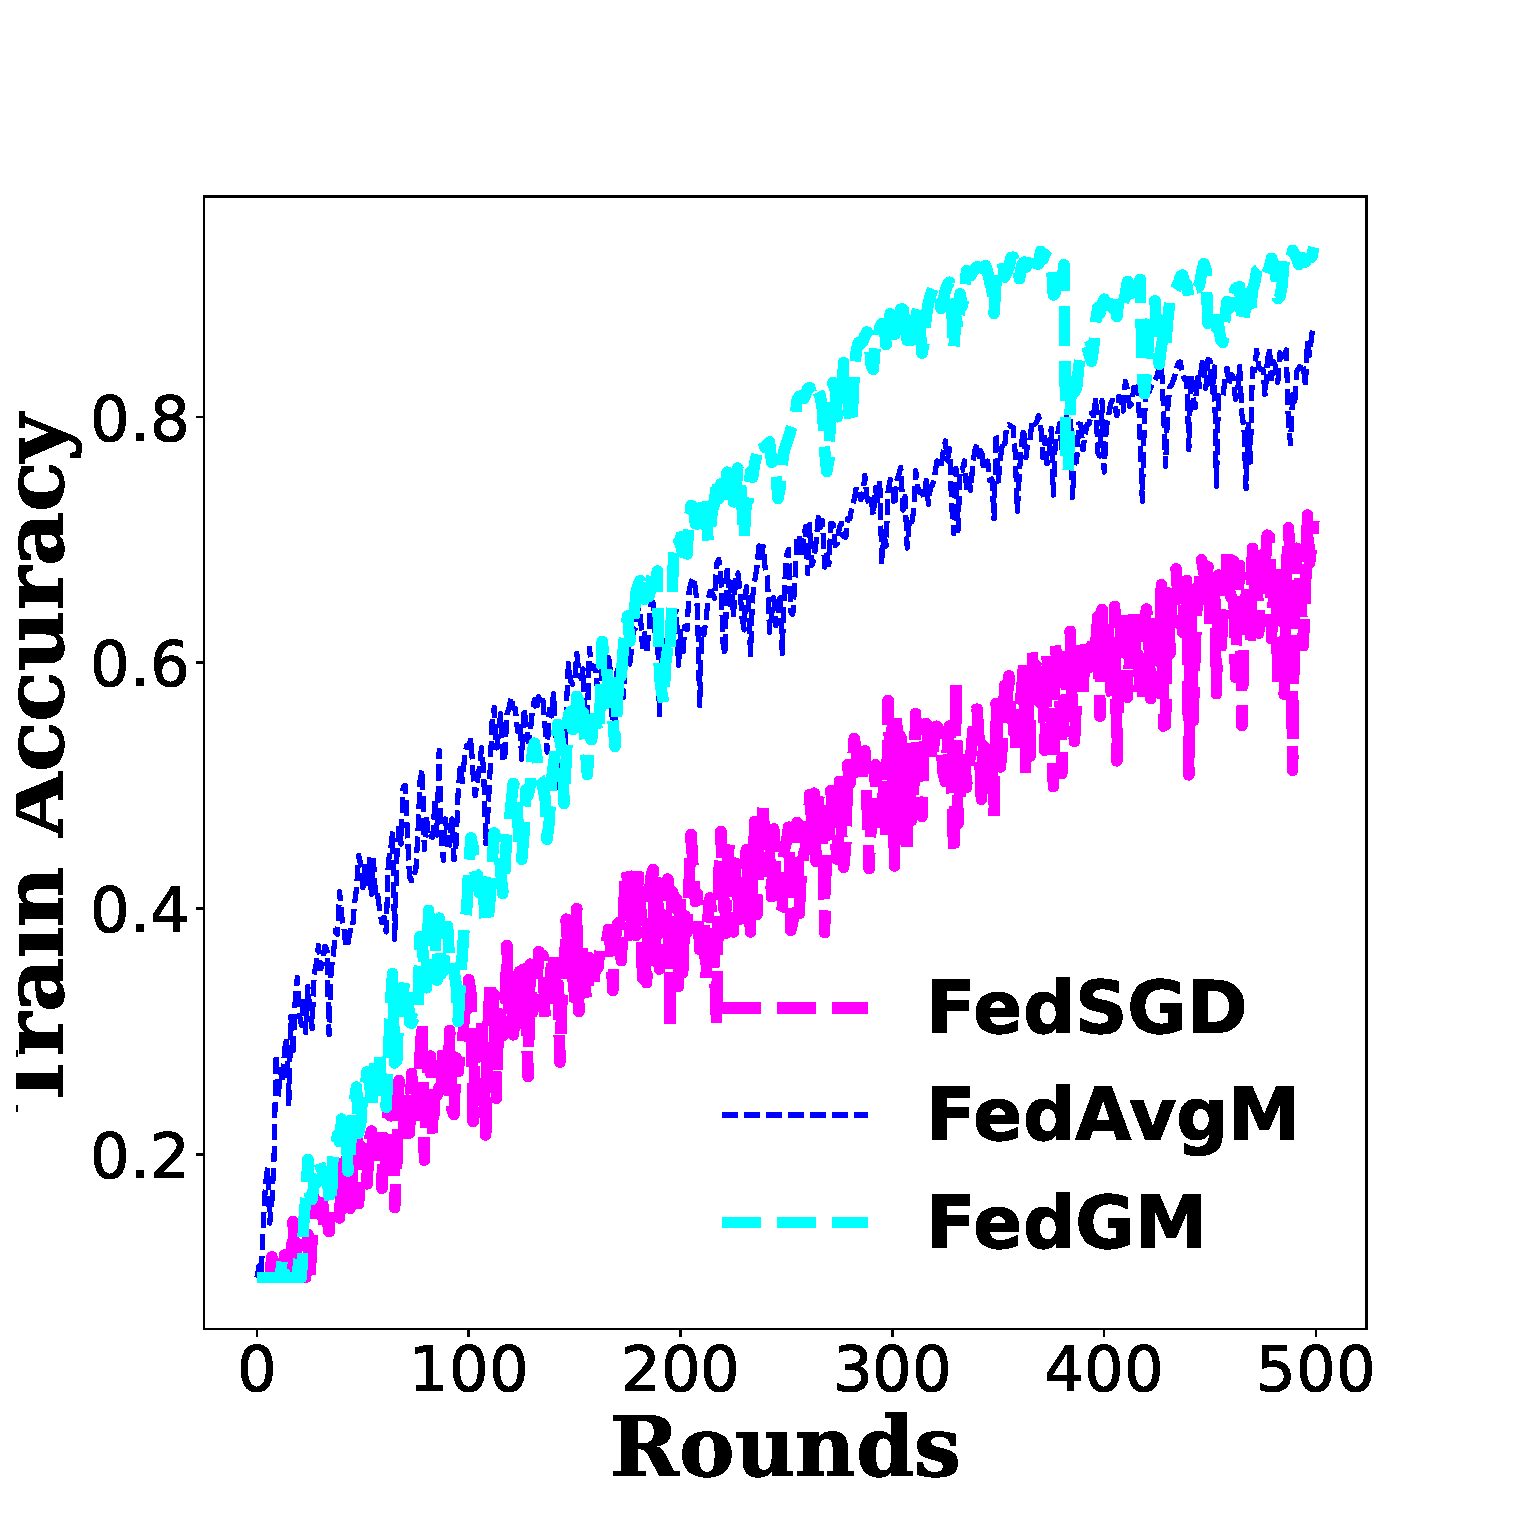
\includegraphics[width=.4\textwidth]{figs/vgg_cifar10_train.eps}
\label{subfig:vgg_cifar10_train}
}
\subfigure{
\hspace{0pt}
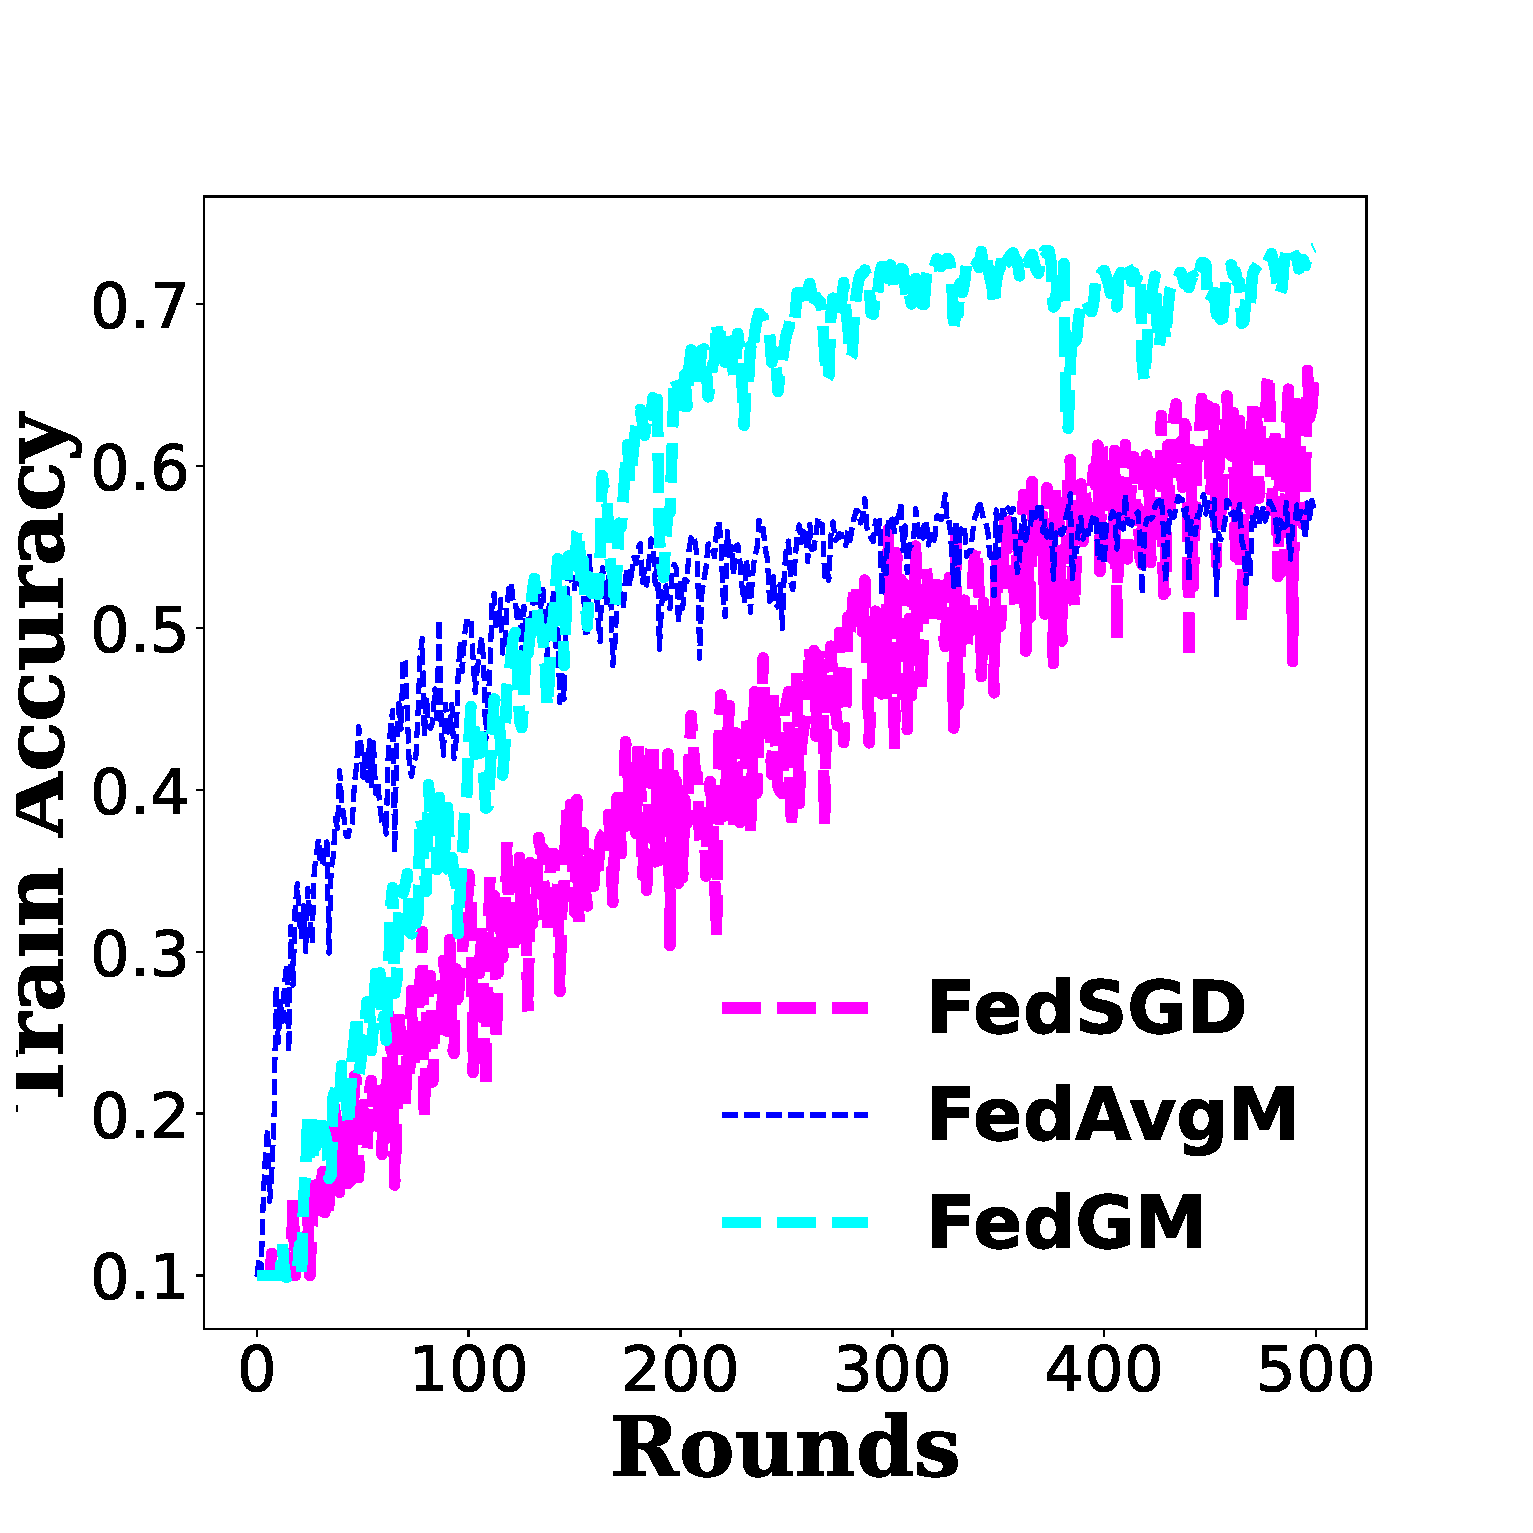
\includegraphics[width=.4\textwidth]{figs/vgg_cifar10_test.eps}
\label{subfig:vgg_cifar10_test}
}
\vspace*{-6pt}
\caption{\ref{subfig:vgg_cifar10_train} Training and \ref{subfig:vgg_cifar10_test} Testing Curve for VGG on CIFAR-10.}
\label{fig:cifar10_vgg_result}
\end{figure}

Figure \ref{fig:cifar10_resnet_various_niid_result} shows the results for ResNet on CIFAR-10 with FedGM and FedAvg with different concentration parameters $\alpha=0.3$ and $\alpha=0.5$ (i.e. \textit{non-i.i.d.}). We perform a similar grid search as in Section \ref{subsec:exp_fedgm}. We could observe the superiority of FedGM compared to FedAvg is consistent with different levels of \textit{non i.i.d.}.


\begin{figure}[h]
\vspace*{-6pt}
\centering
\subfigure{
\hspace{0pt}
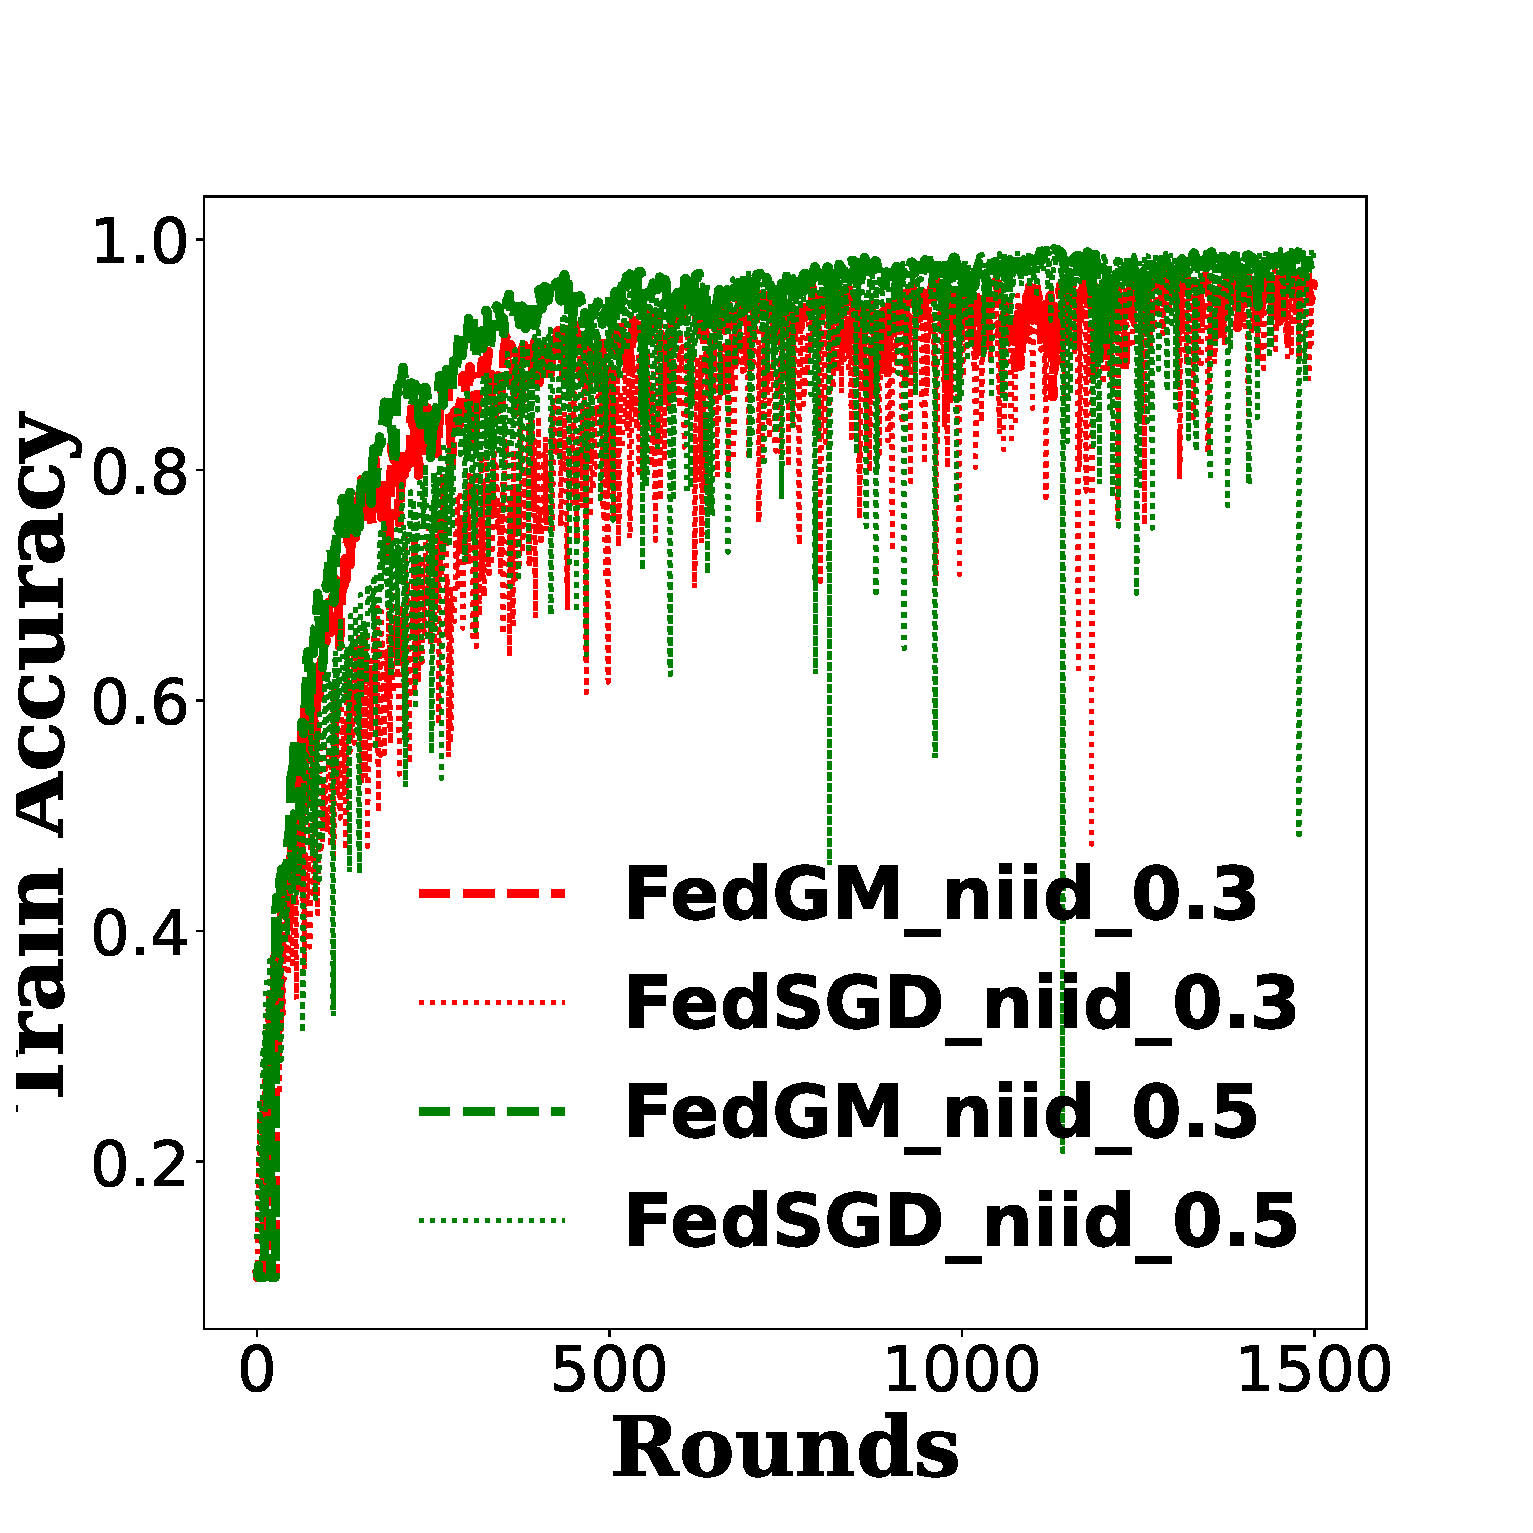
\includegraphics[width=.4\textwidth]{figs/resnet_cifar10_train_various_iid.eps}
\label{subfig:resnet_cifar10_train_various_iid}
}
\subfigure{
\hspace{0pt}
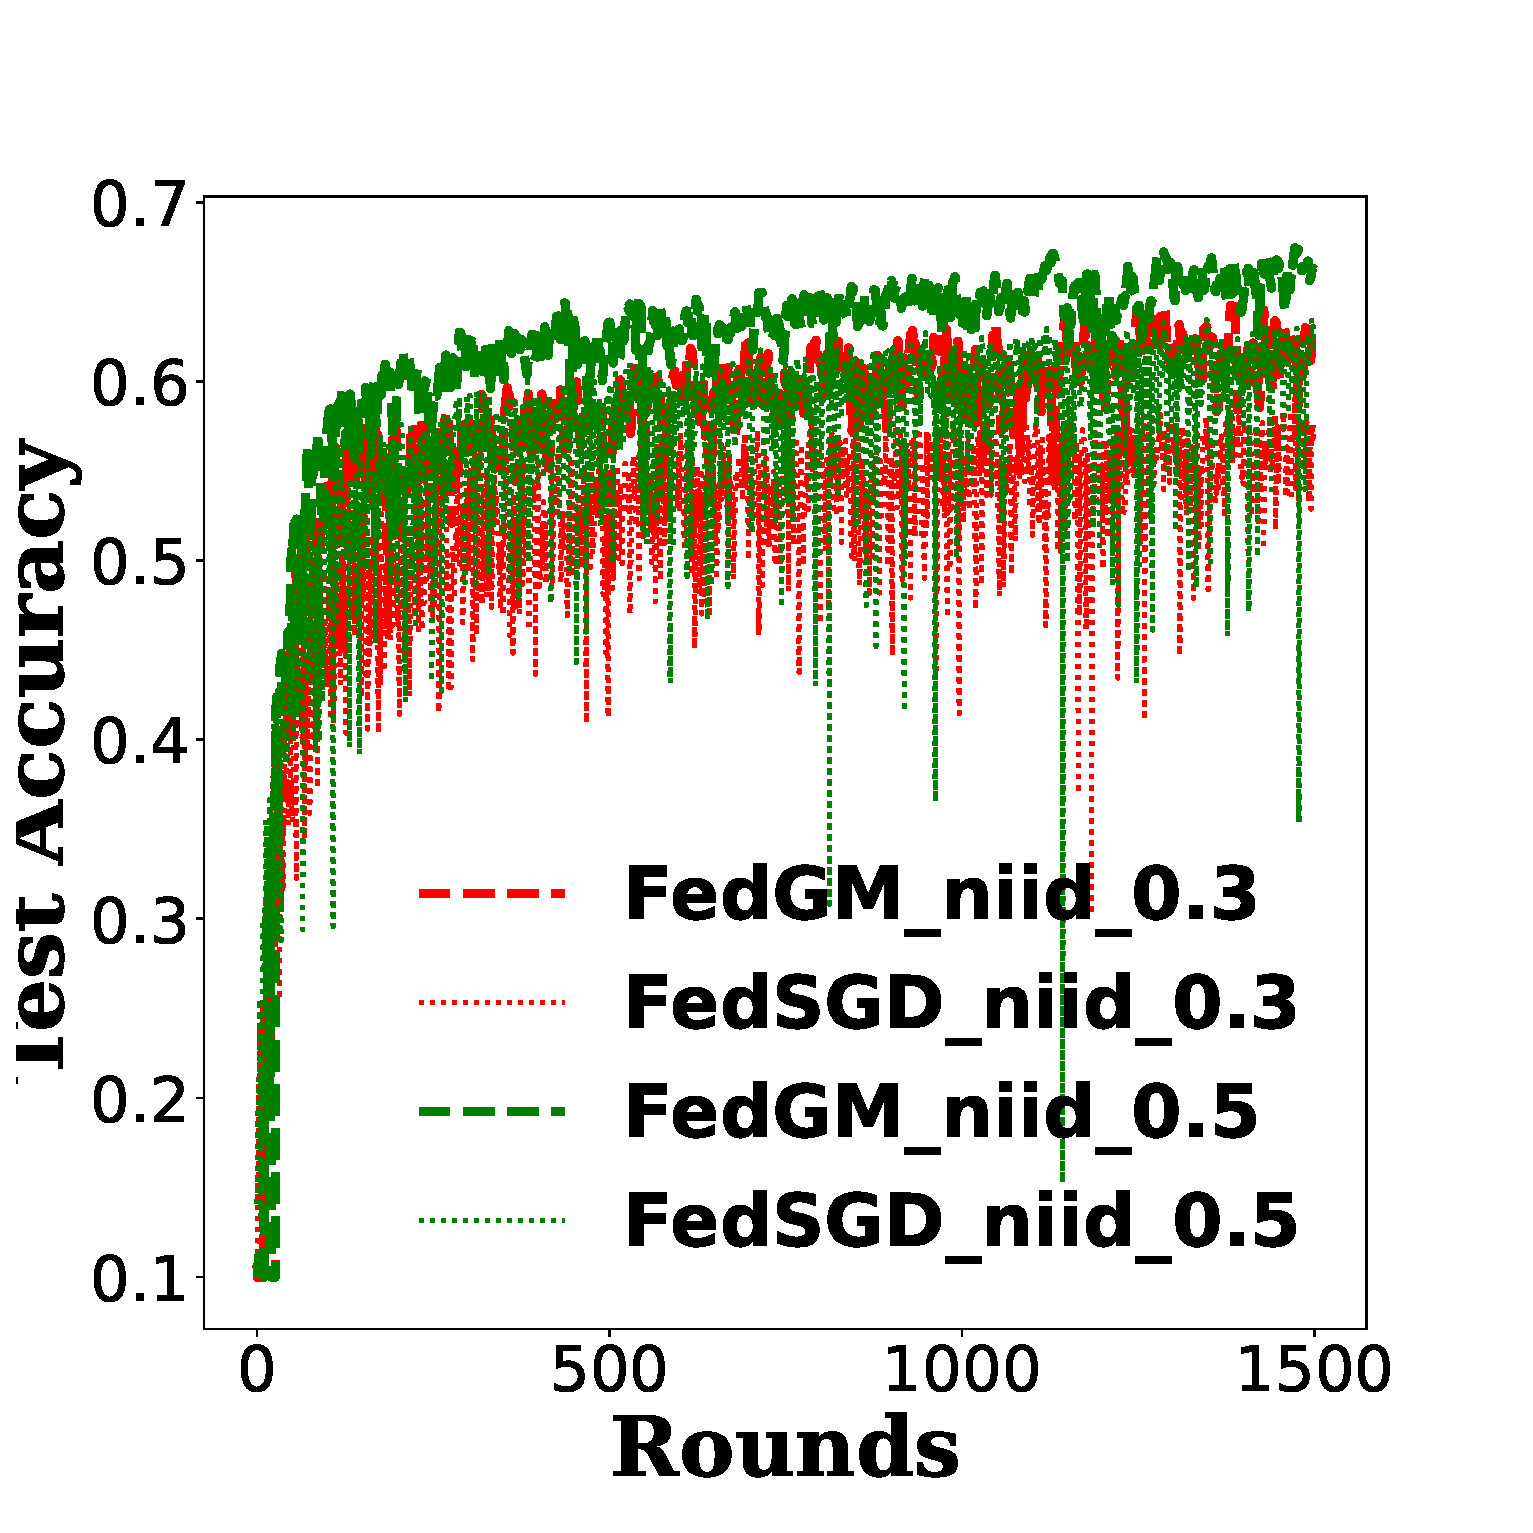
\includegraphics[width=.4\textwidth]{figs/resnet_cifar10_test_various_iid.eps}
\label{subfig:resnet_cifar10_test_various_iid}
}
\vspace*{-6pt}
\caption{\ref{subfig:resnet_cifar10_train_various_iid} Training and \ref{subfig:resnet_cifar10_test_various_iid} Testing Curve for ResNet on CIFAR-10 with Various Levels of Heterogeneity}
\label{fig:cifar10_resnet_various_niid_result}
\end{figure}

\textbf{Verifying Remark \ref{remark:full_participation_why_momentum_helps}}

Remark \ref{remark:full_participation_why_momentum_helps} hypothesizes FedGM could converge with a large $\eta$ while FedAvg would diverge easily with an only moderately large server learning rate. The reason is that $\eta$ acts like a multiplier to client learning rate $\eta_l$ in FedAvg, while in FedGM, $\beta$ and $\nu$ act as a buffer that could absorb the impact from a large $\eta$. We verify this remark here.

Figure \ref{fig:fedavg_various_lr_result} shows the results for ResNet on CIFAR-10 with FedAvg but different learning rates $\eta=1.0$, $\eta=2.0$, and $\eta=3.0$. We could see FedAvg experiences an unstable convergence even when $\eta=2.0$ and completely divergent when $\eta=3.0$.

\begin{figure}[h]
\vspace*{-6pt}
\centering
\subfigure{
\hspace{0pt}
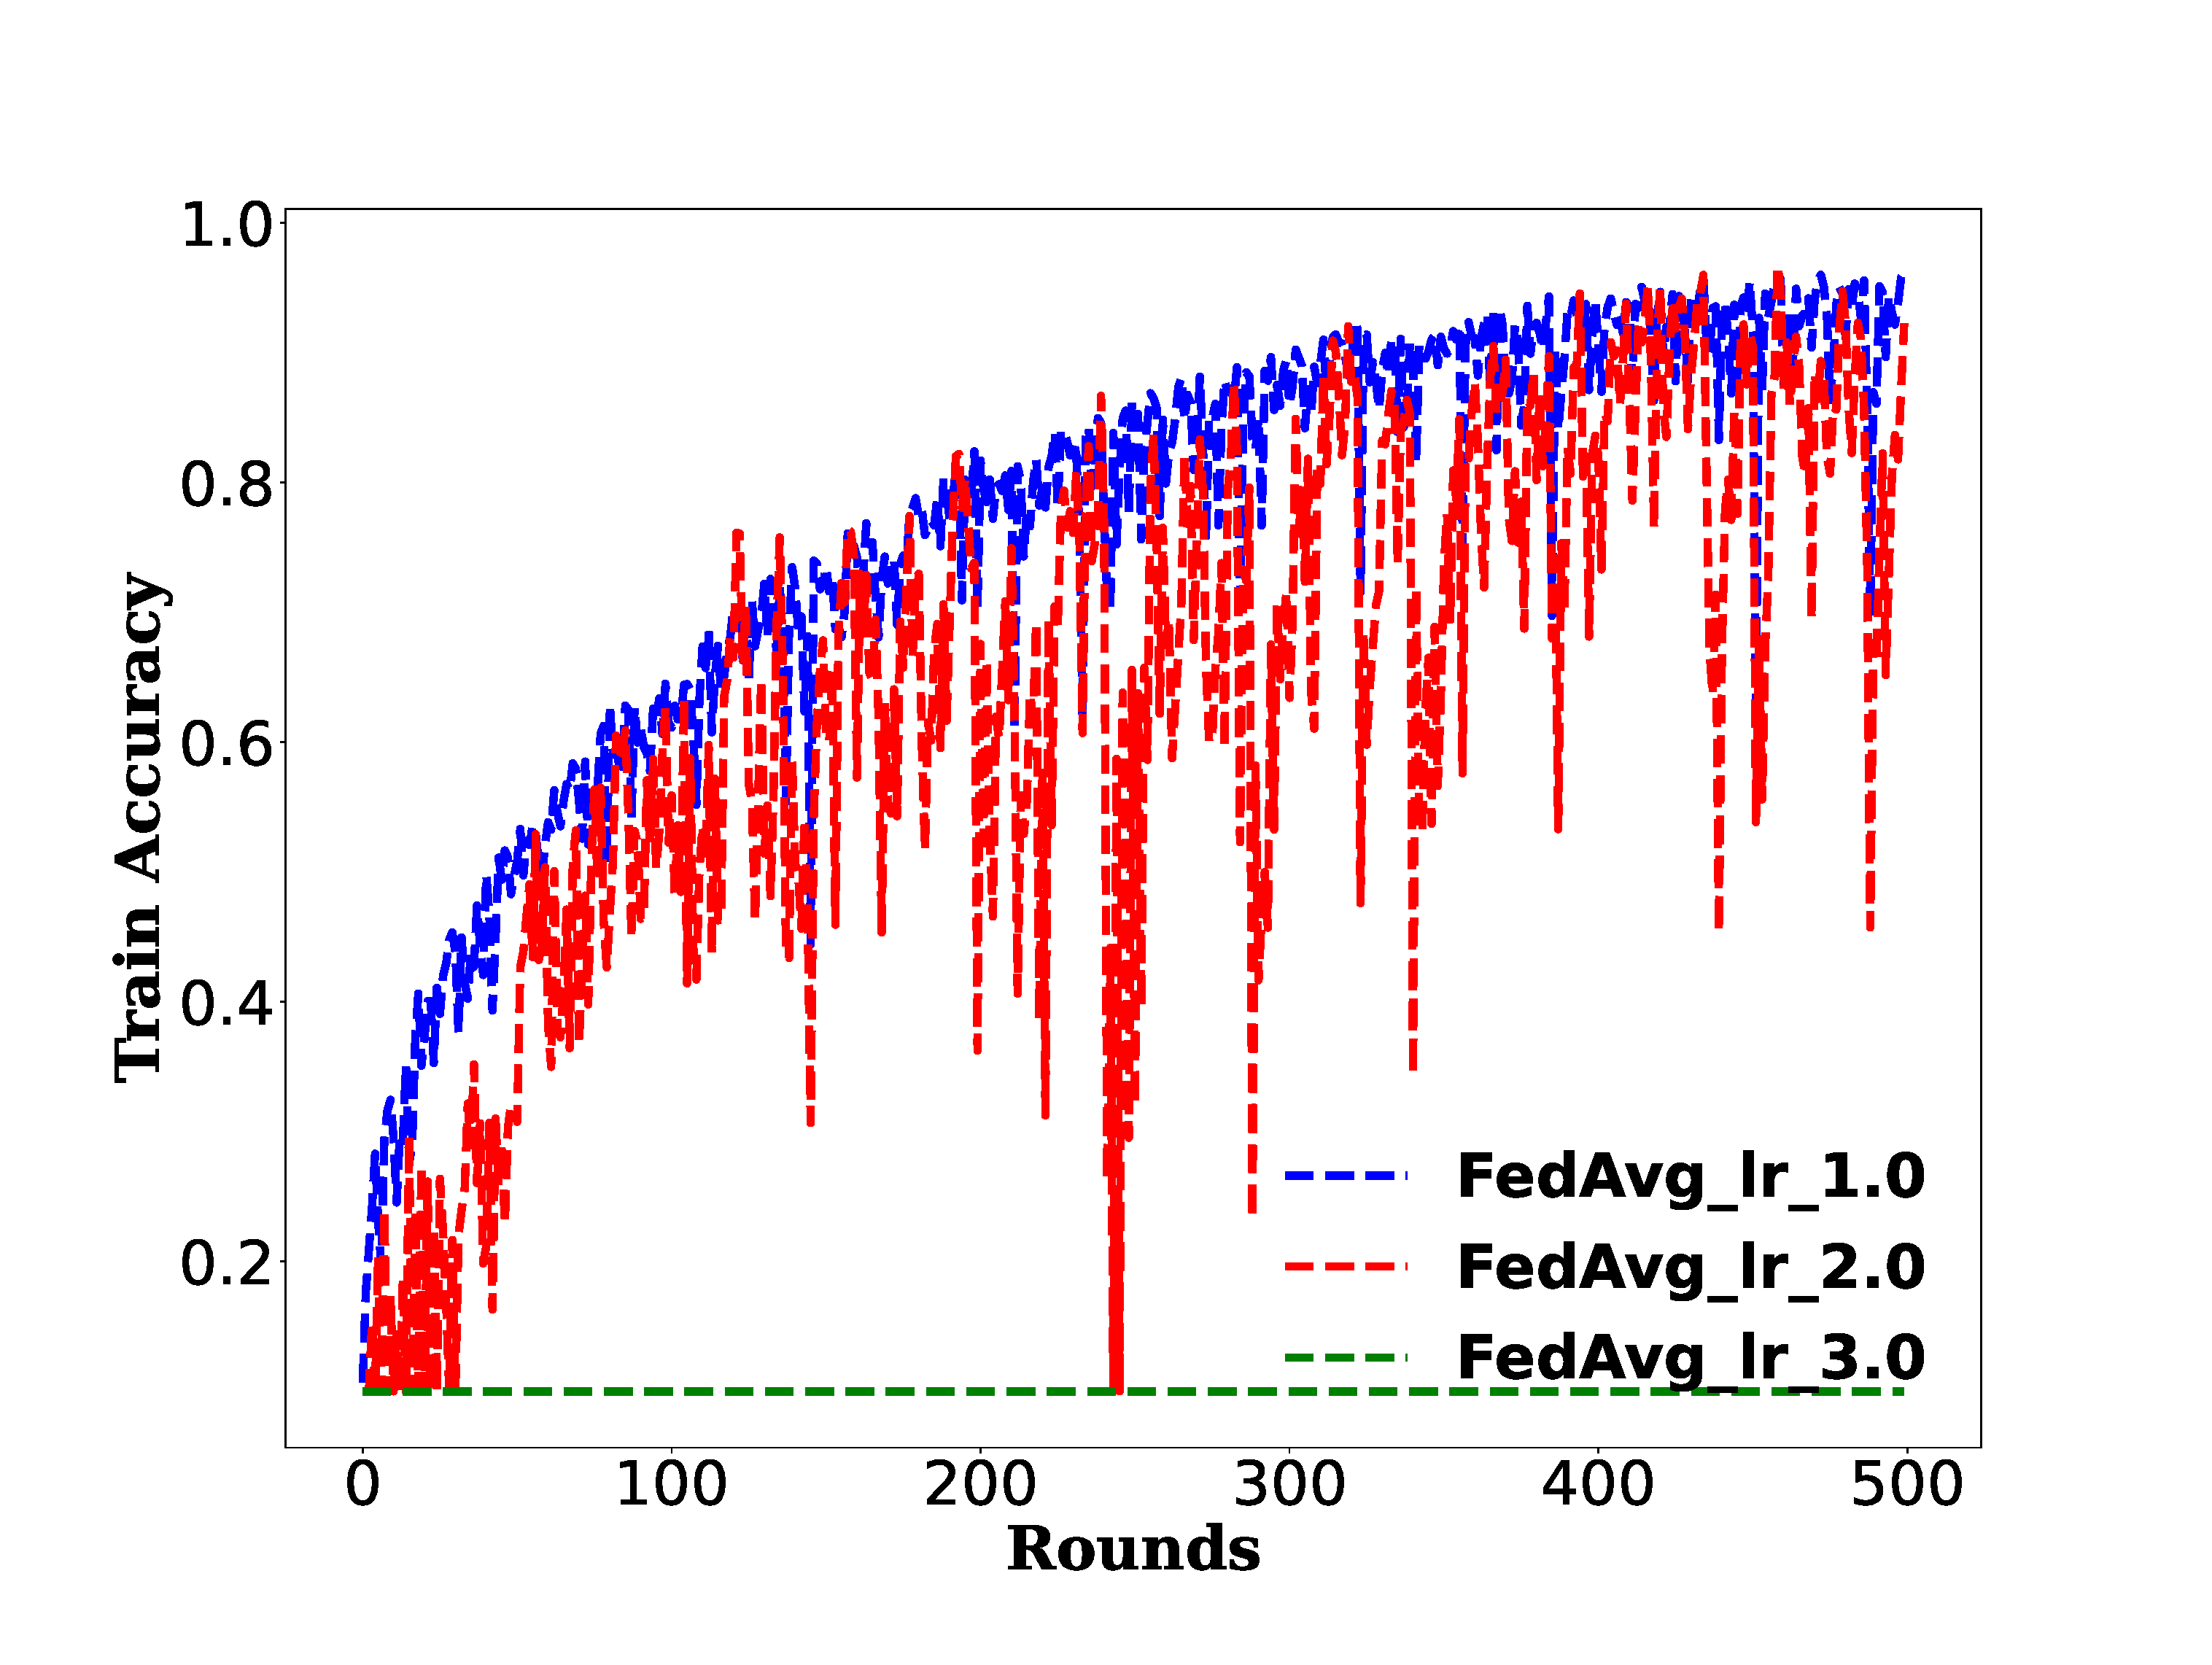
\includegraphics[width=.35\textwidth]{figs/FedAvg_various_lr_train.eps}
\label{subfig:fedavg_various_lr_train}
}
\subfigure{
\hspace{0pt}
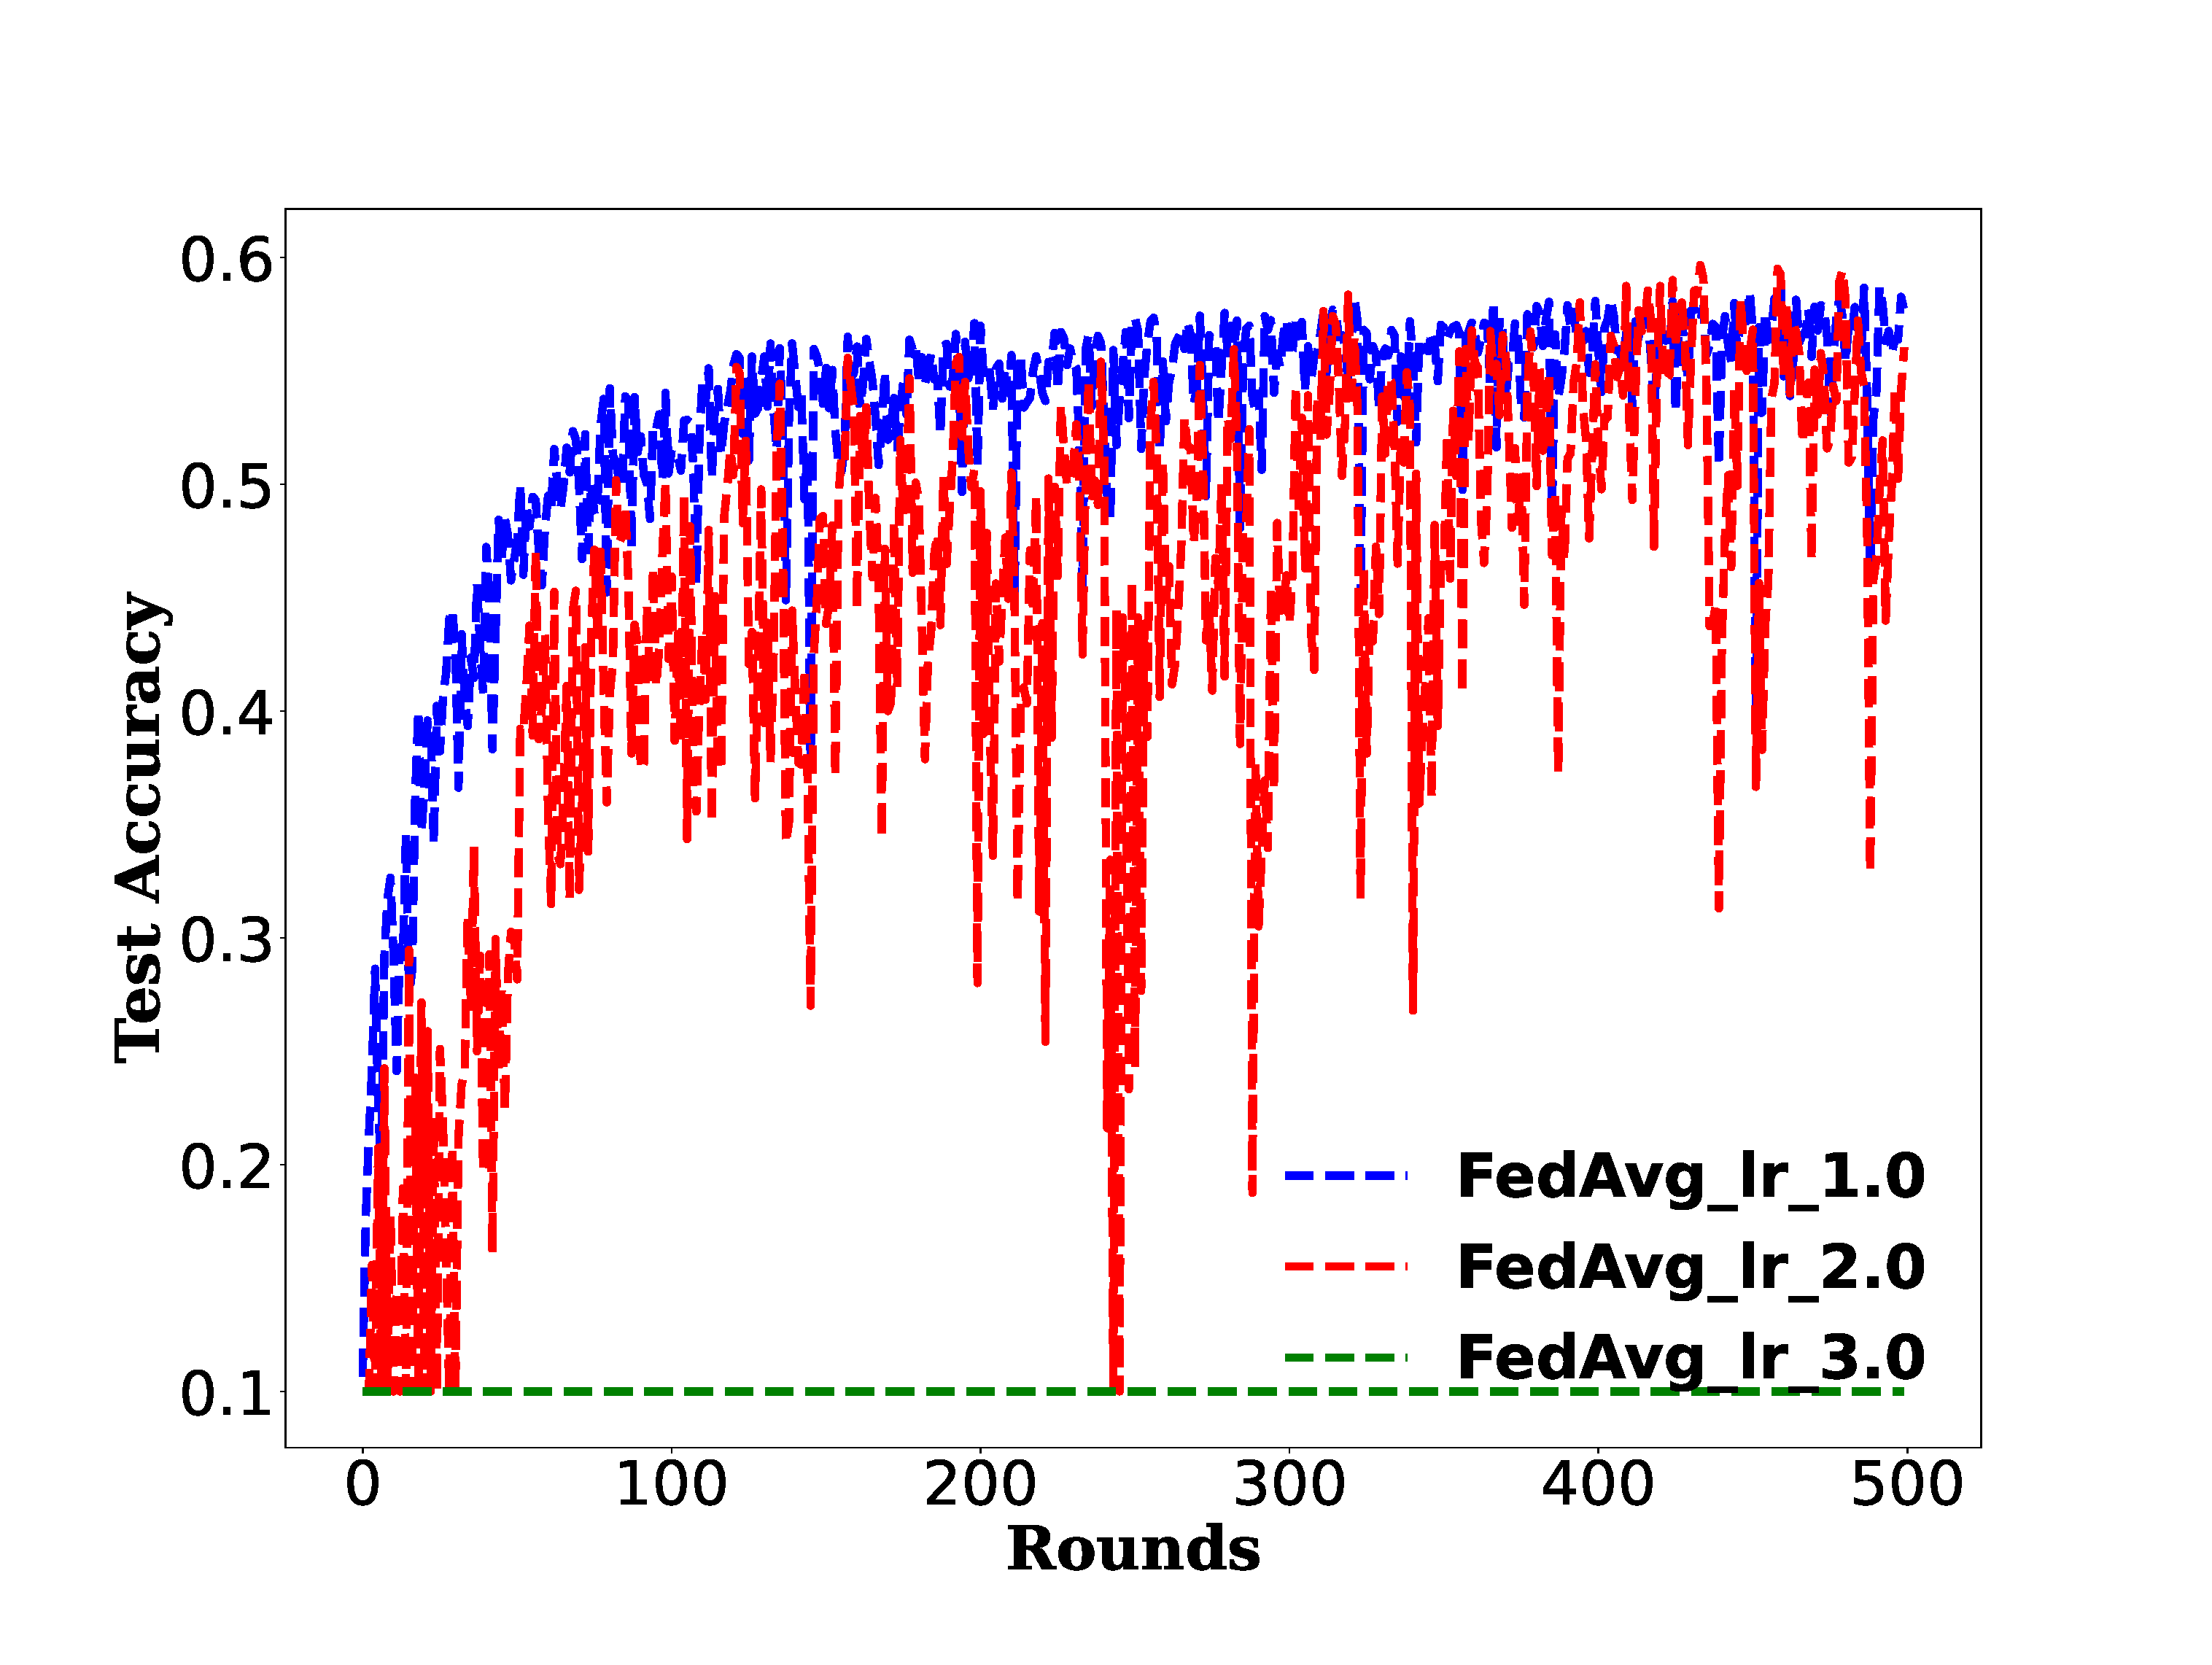
\includegraphics[width=.35\textwidth]{figs/FedAvg_various_lr_test.eps}
\label{subfig:fedavg_various_lr_test}
}
\vspace*{-6pt}
\caption{\ref{subfig:fedavg_various_lr_train} Training and \ref{subfig:fedavg_various_lr_test} Testing Curve for FedAvg with various server learning rates $\eta$.}
\label{fig:fedavg_various_lr_result}
\end{figure}

Figure \ref{fig:fedgm_various_lr_result} shows the results for FedGM but different learning rates $\eta=1.0$, $\eta=3.0$, and $\eta=5.0$. All experimental settings are identical to Figure \ref{fig:fedavg_various_lr_result} except for the difference between FedAvg and FedGM. We could see FedGM sustains a much larger $\eta$ compared to FedAvg. It could converge and even accelerate with $\eta=5.0$ compared to FedAvg baseline.


\begin{figure}[h]
\vspace*{-6pt}
\centering
\subfigure{
\hspace{0pt}
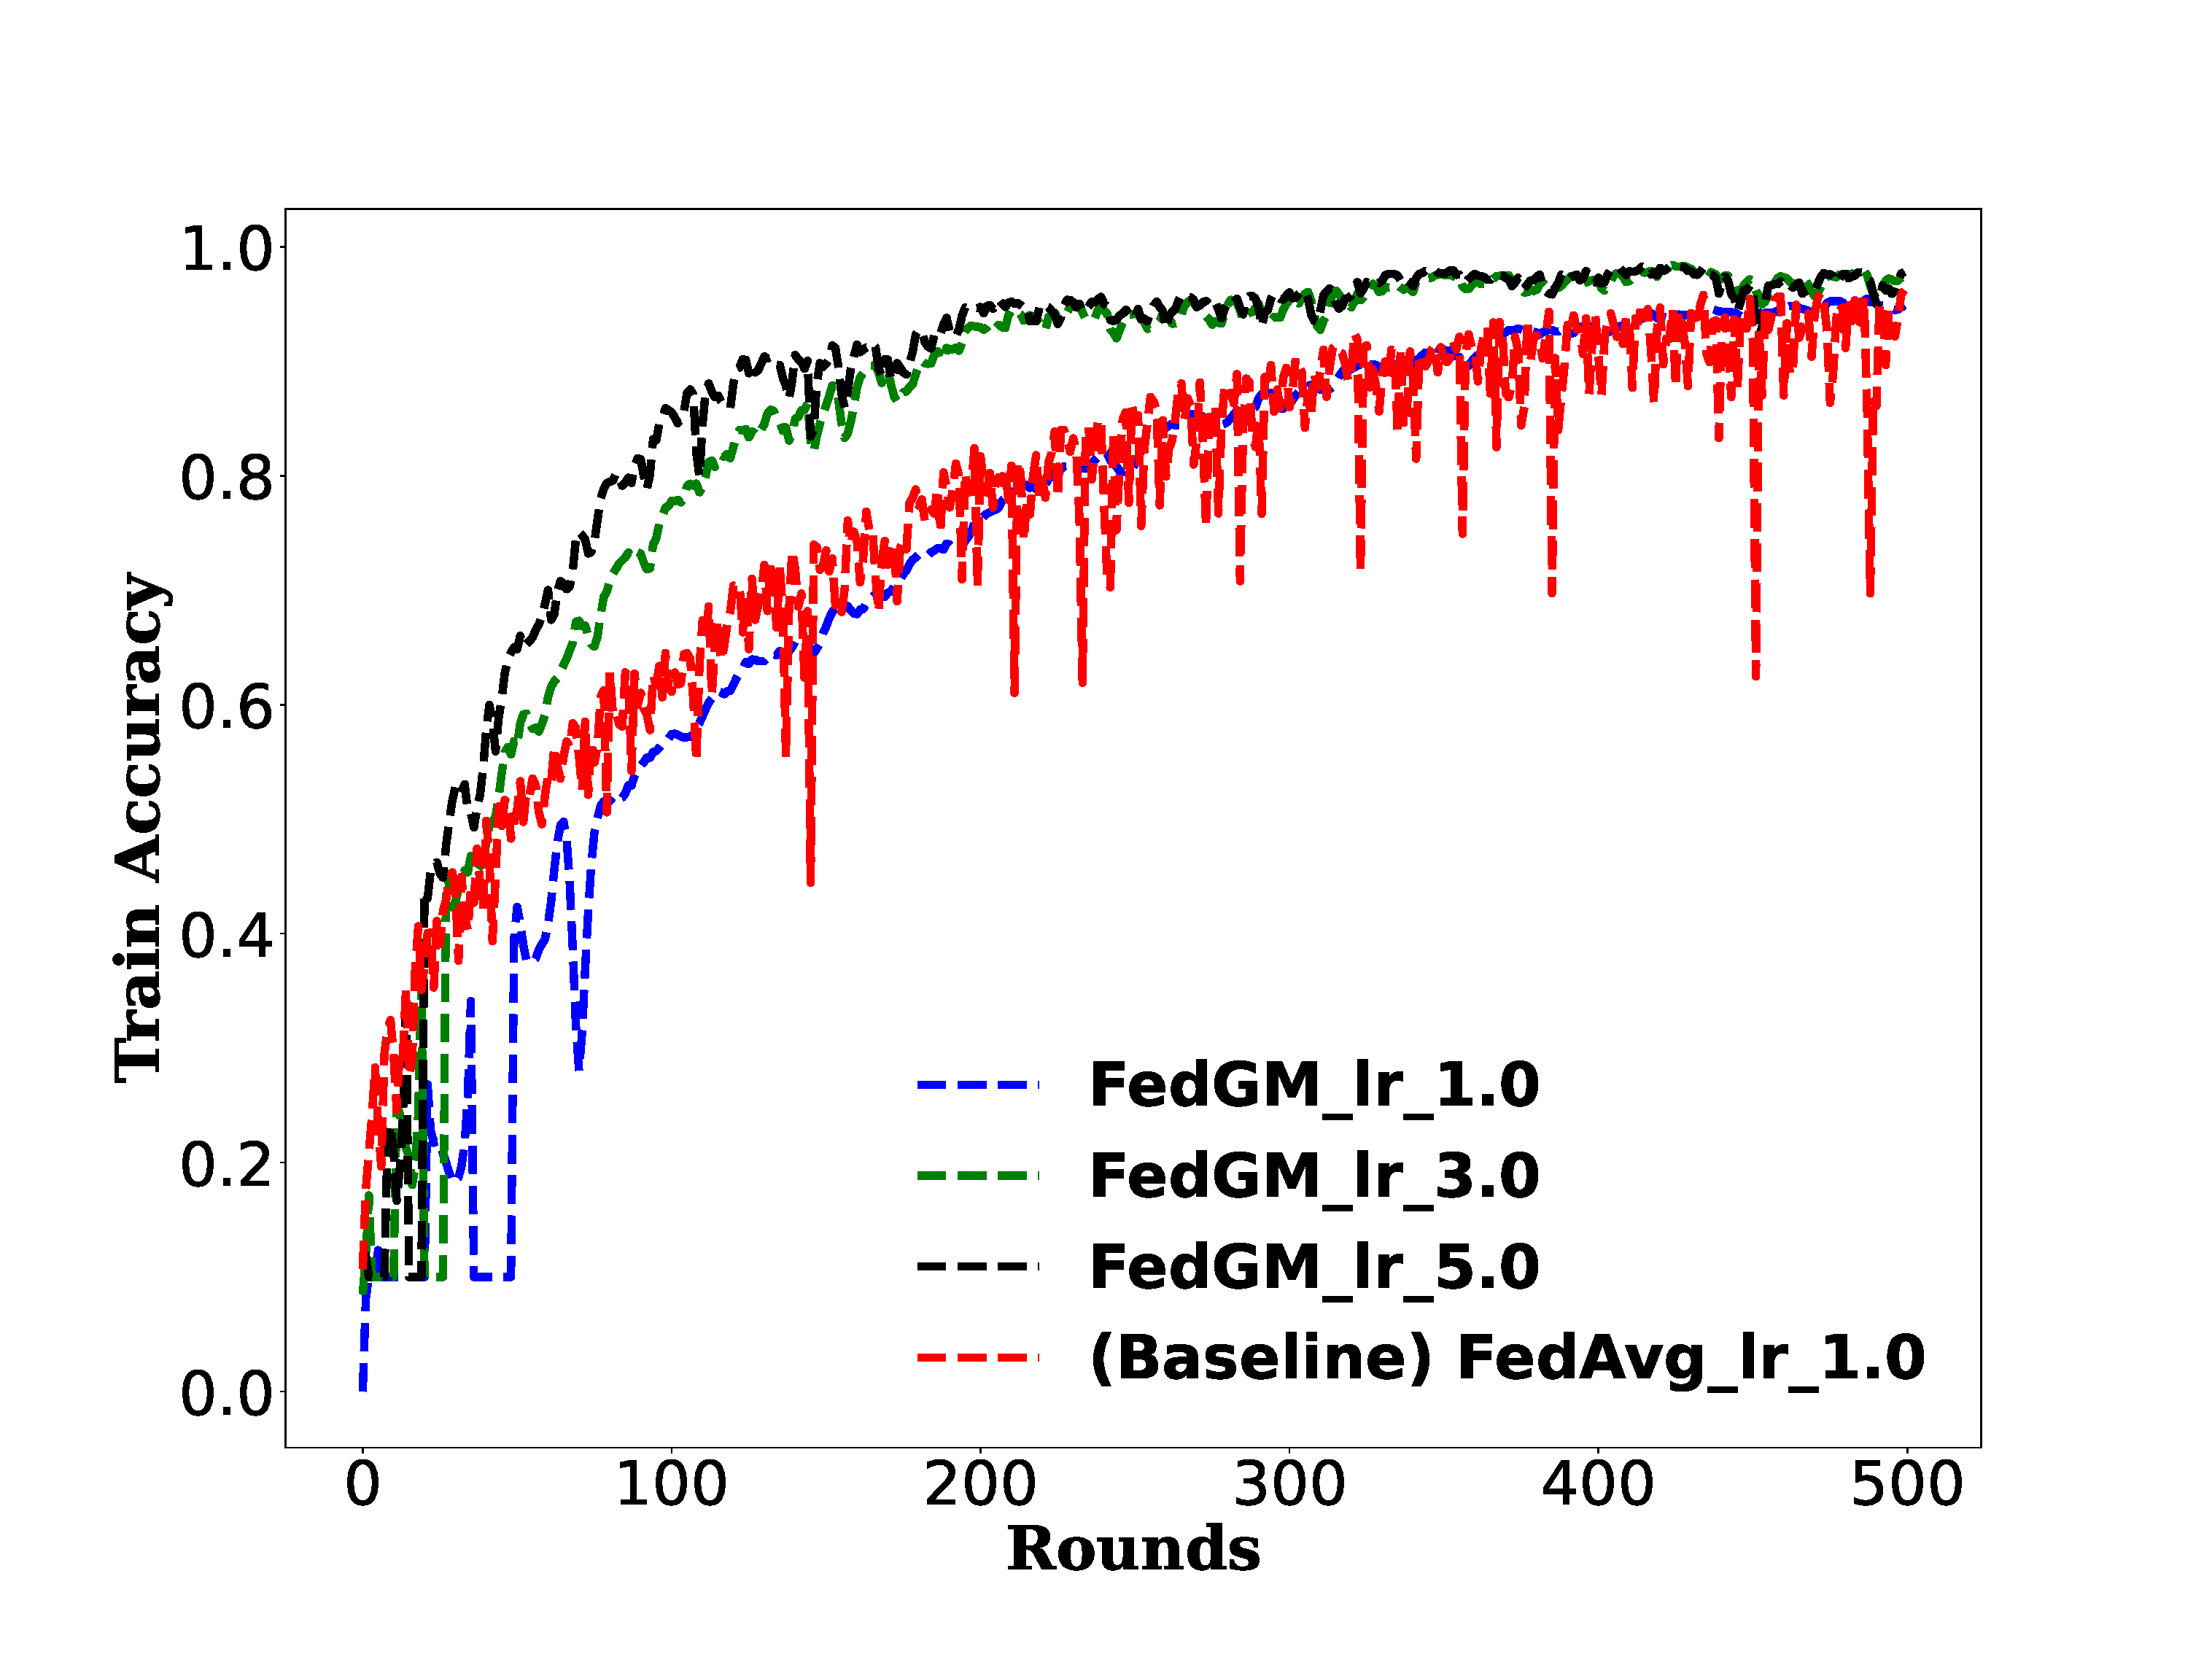
\includegraphics[width=.35\textwidth]{figs/FedGM_various_lr_train.eps}
\label{subfig:fedgm_various_lr_train}
}
\subfigure{
\hspace{0pt}
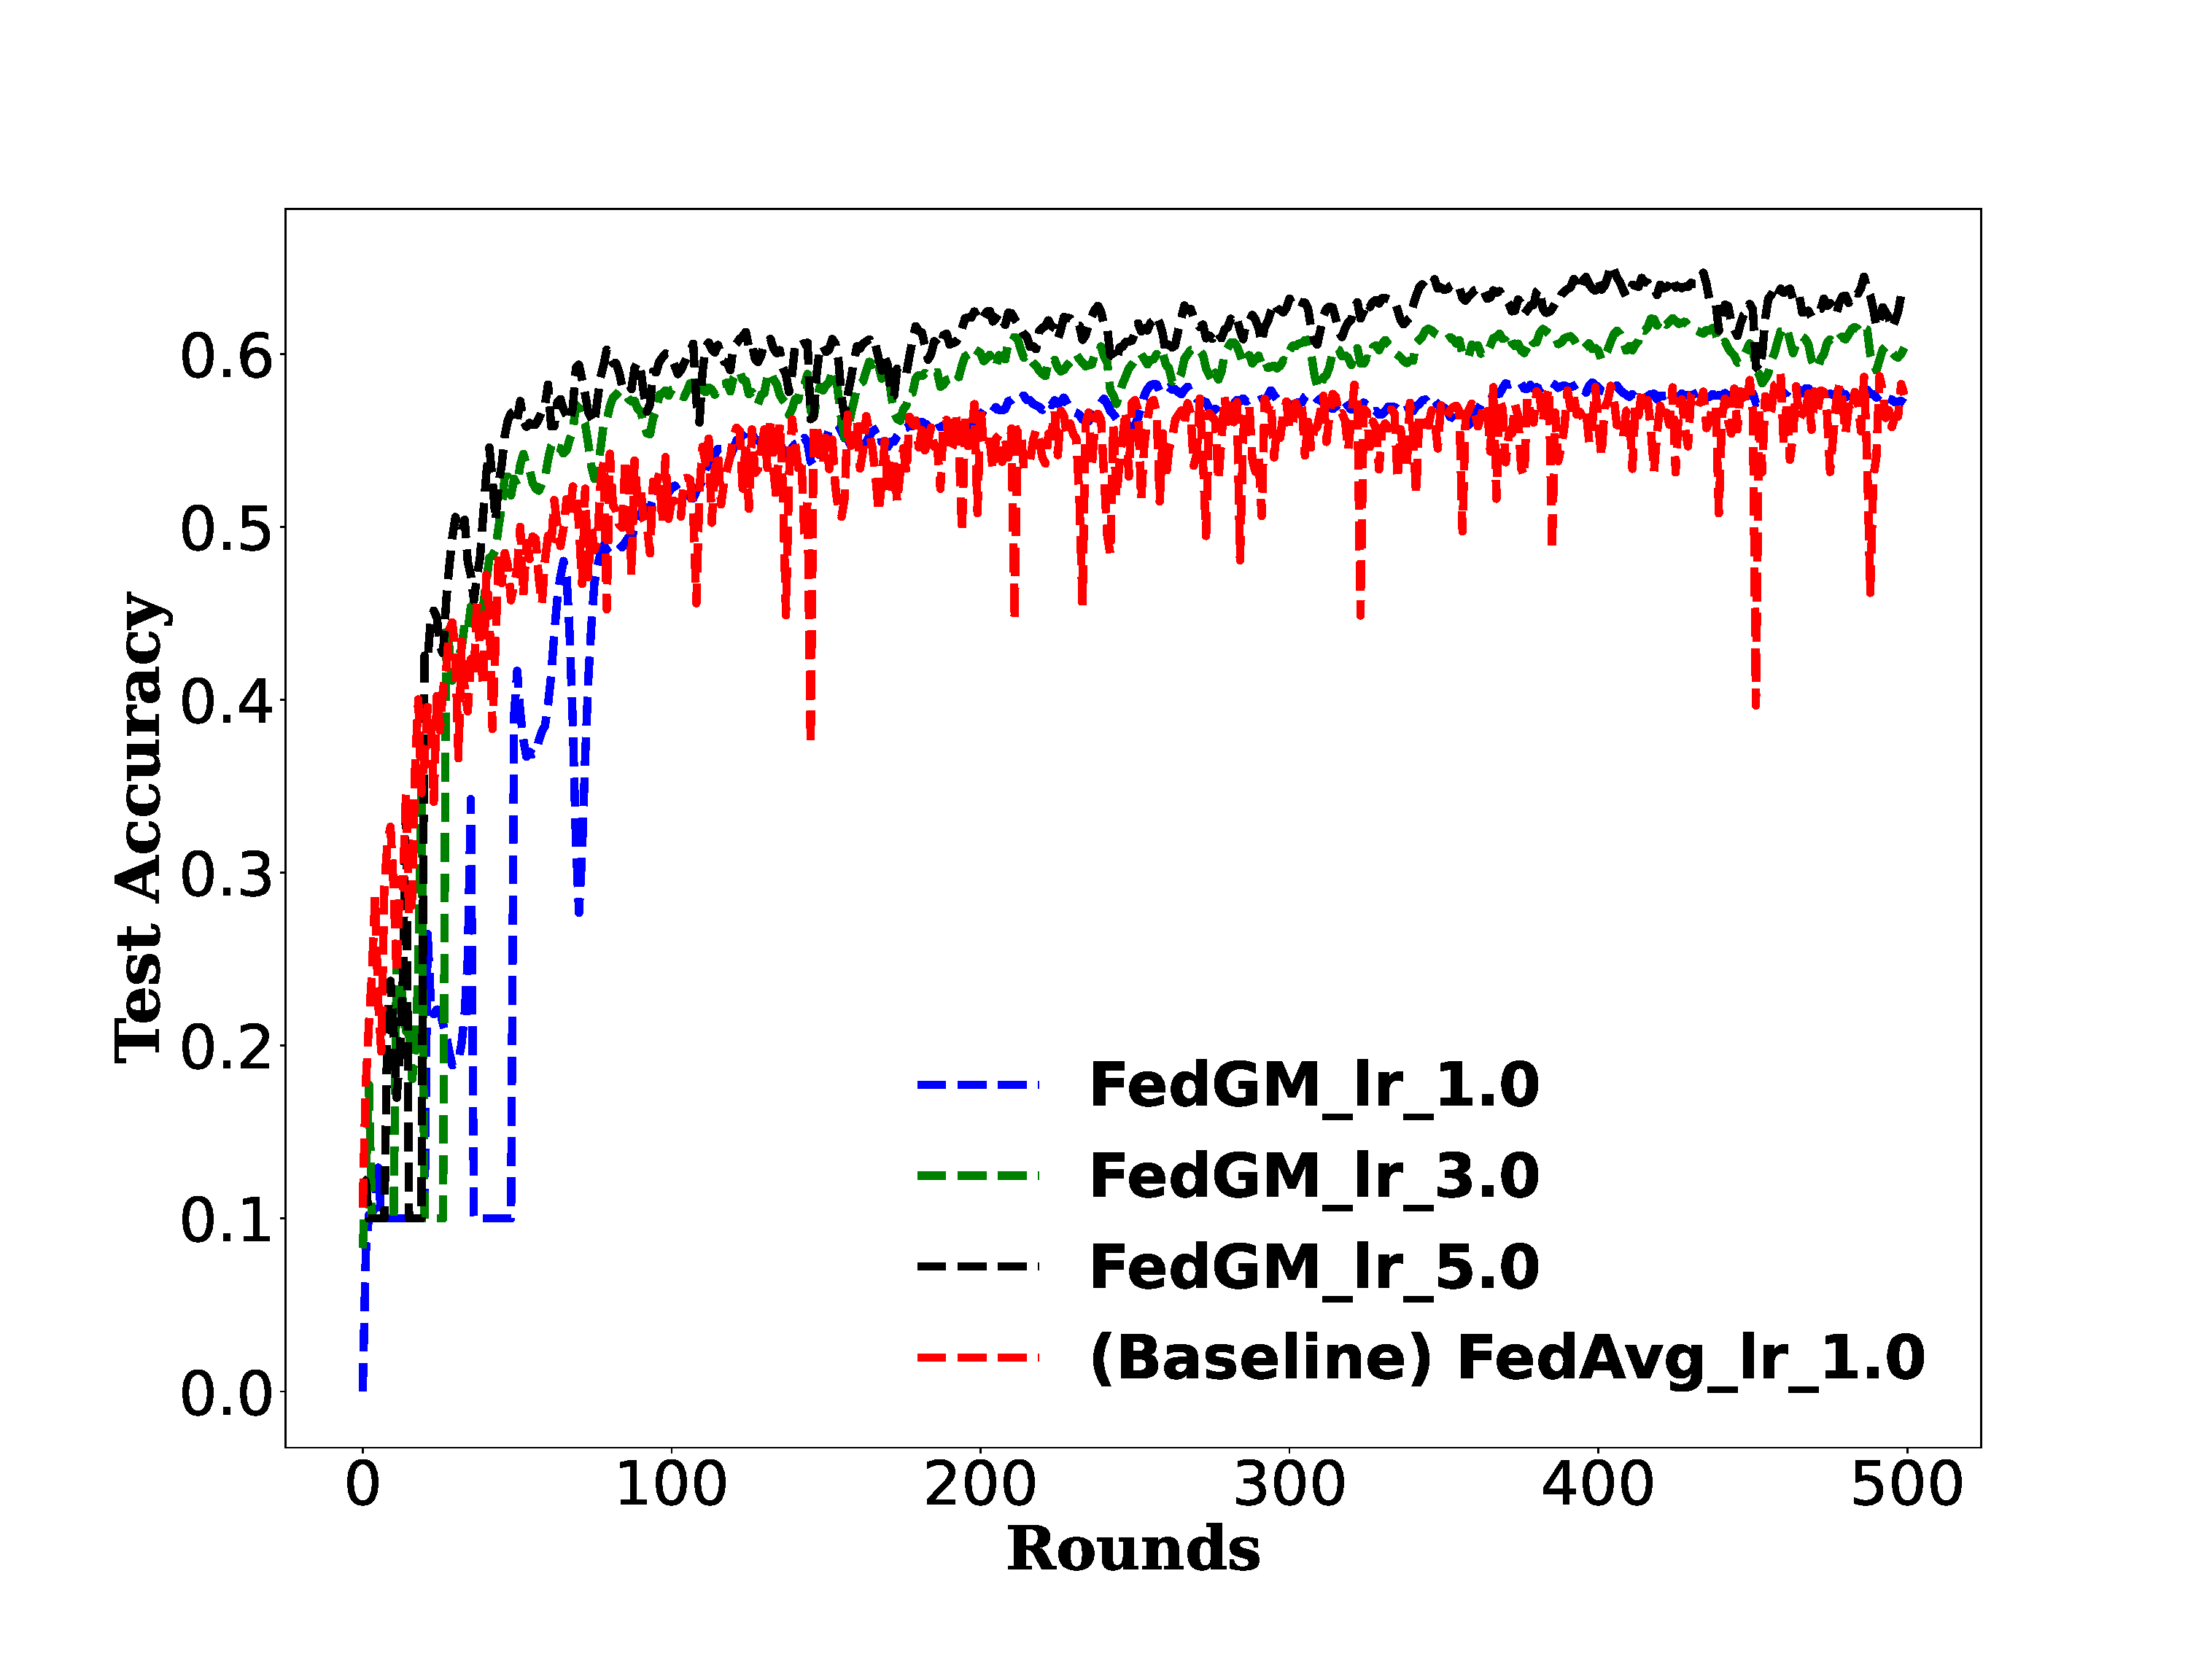
\includegraphics[width=.35\textwidth]{figs/FedGM_various_lr_test.eps}
\label{subfig:fedgm_various_lr_test}
}
\vspace*{-6pt}
\caption{\ref{subfig:fedgm_various_lr_train} Training and \ref{subfig:fedgm_various_lr_test} Testing Curve for FedGM with various server learning rates $\eta$.}
\label{fig:fedgm_various_lr_result}
\end{figure}


\subsection{More Experiments in Section \ref{subsec:exp_multistage_fedgm}}
\label{subsec:more_exp_multistage_appendix}

Figure \ref{fig:fedgm_various_lr_early_late_result} motivates our multistage FedGM. We run ResNet on CIFAR-10 with FedGM but different learning rates $\eta=1.0$, $\eta=2.0$, and $\eta=5.0$ for 2000 rounds. We fix $\beta=\nu=0.95$ for expository purpose. We could see in early rounds (i.e. the first 500 rounds), $\eta=5.0$ has advantages that it converges faster than small $\eta=1.0$. However, $\eta=1.0$ is much more stable than  $\eta=5.0$ in the last 500 rounds when they all get nearly perfect training accuracy. This is consistent with the motivation of multistage FedGM, i.e. large initial $\eta$ benefits exploration, while small later $\eta$ benefits exploitation, and multistage scheduler obtains a balance.



\begin{figure}[h]
\vspace*{-6pt}
\centering
\subfigure{
\hspace{0pt}
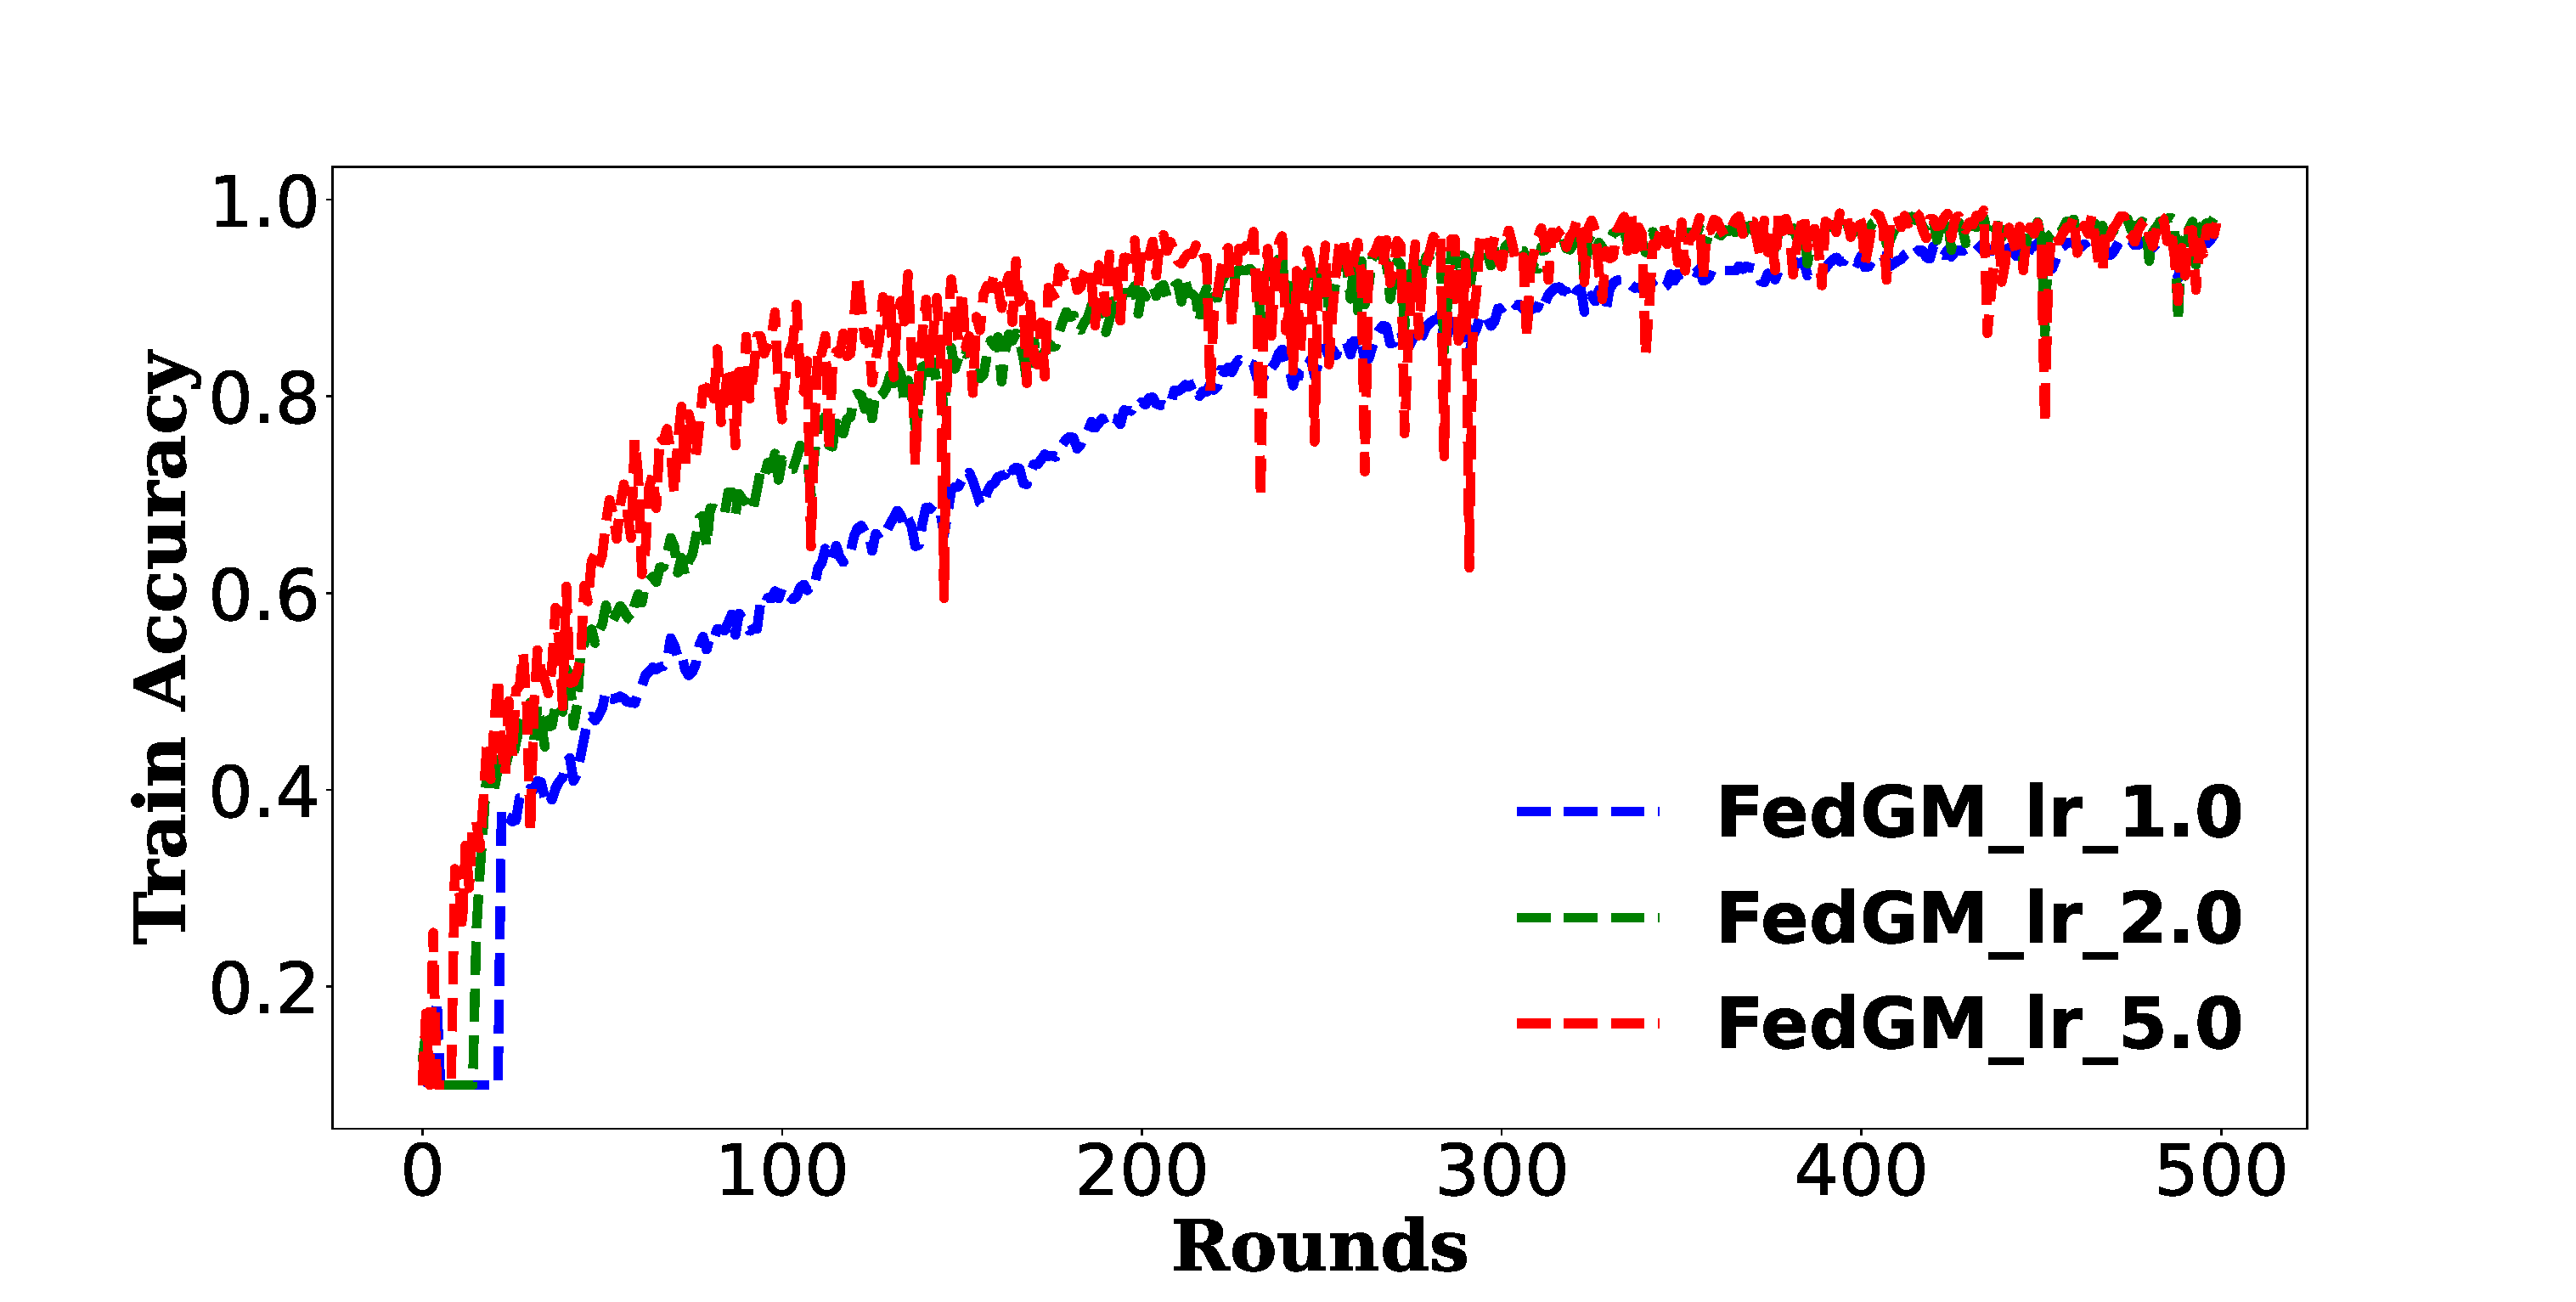
\includegraphics[width=.42\textwidth]{figs/FedGM_various_lr_initial_train.eps}
\label{subfig:fedgm_various_lr_initial_train}
}
\subfigure{
\hspace{0pt}
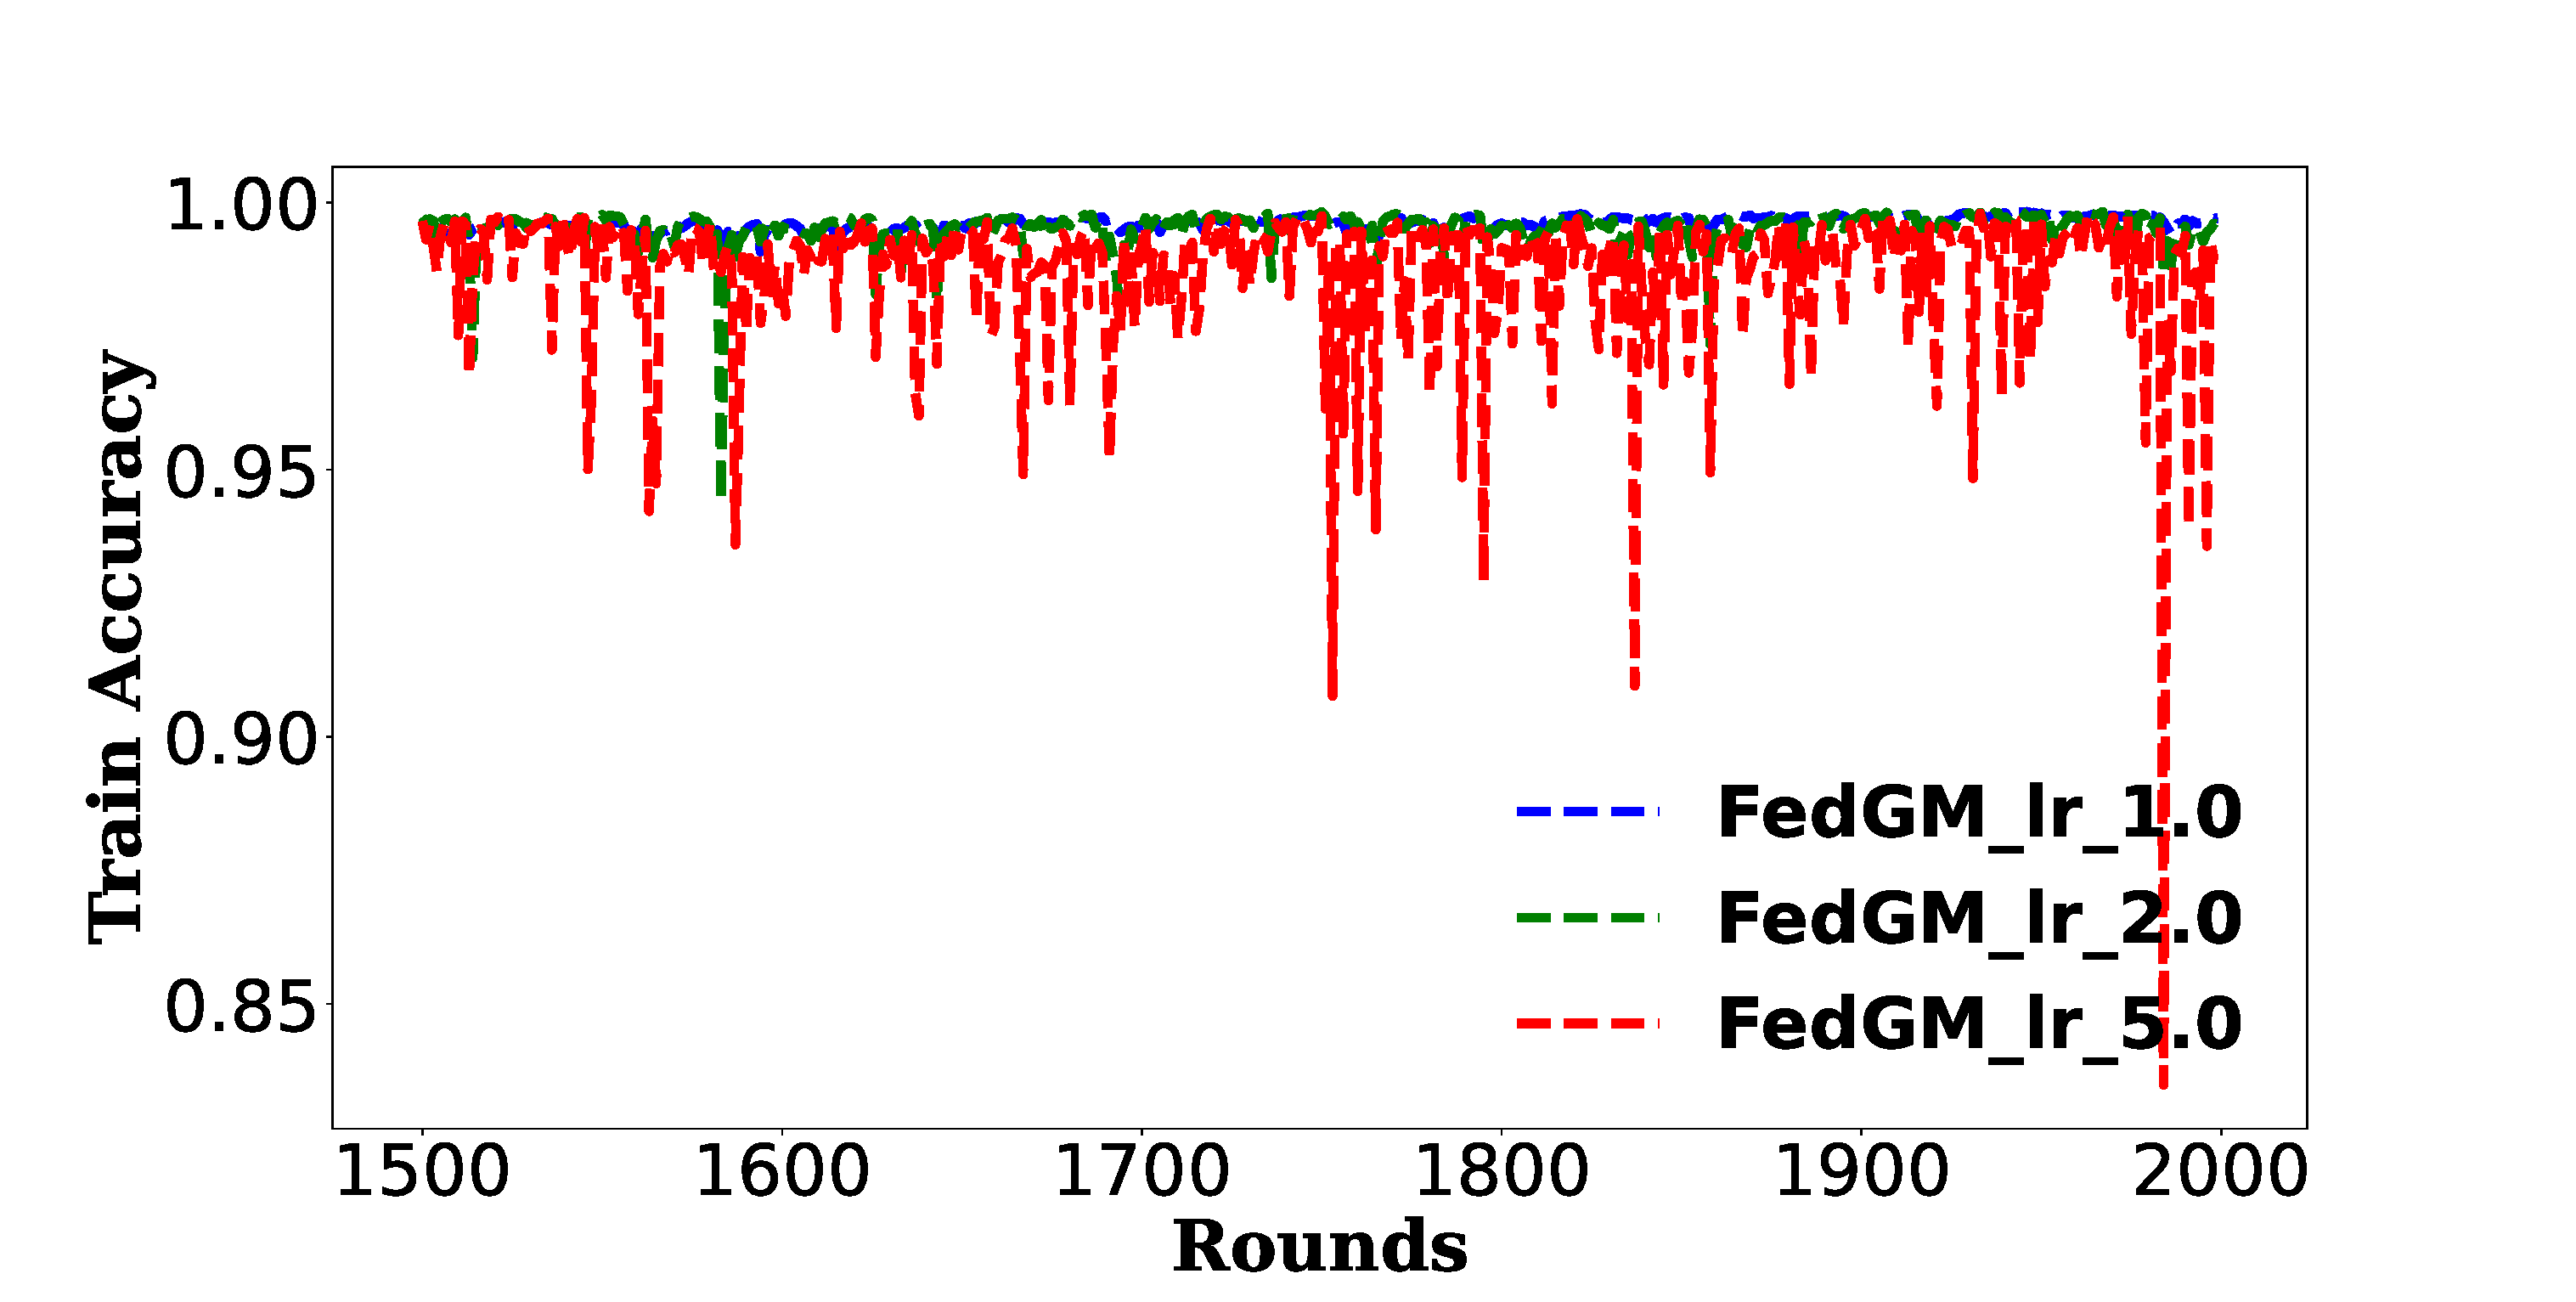
\includegraphics[width=.42\textwidth]{figs/FedGM_various_lr_late_train.eps}
\label{subfig:fedgm_various_lr_late_train}
}
\vspace*{-6pt}
\caption{Training Curves for FedGM with various server learning rates $\eta$. \ref{subfig:fedgm_various_lr_initial_train} the first 500 rounds; \ref{subfig:fedgm_various_lr_late_train} the last 500 rounds.}
\label{fig:fedgm_various_lr_early_late_result}
\end{figure}

\iffalse

Figure \ref{fig:resnet_cifar10_multistage_remake} presents the training and testing curves for multistage FedGM that is omitted in Section \ref{subsec:exp_multistage_fedgm} due to page limit.

\begin{figure}[h]
\vspace*{-6pt}
\centering
\subfigure{
\hspace{0pt}
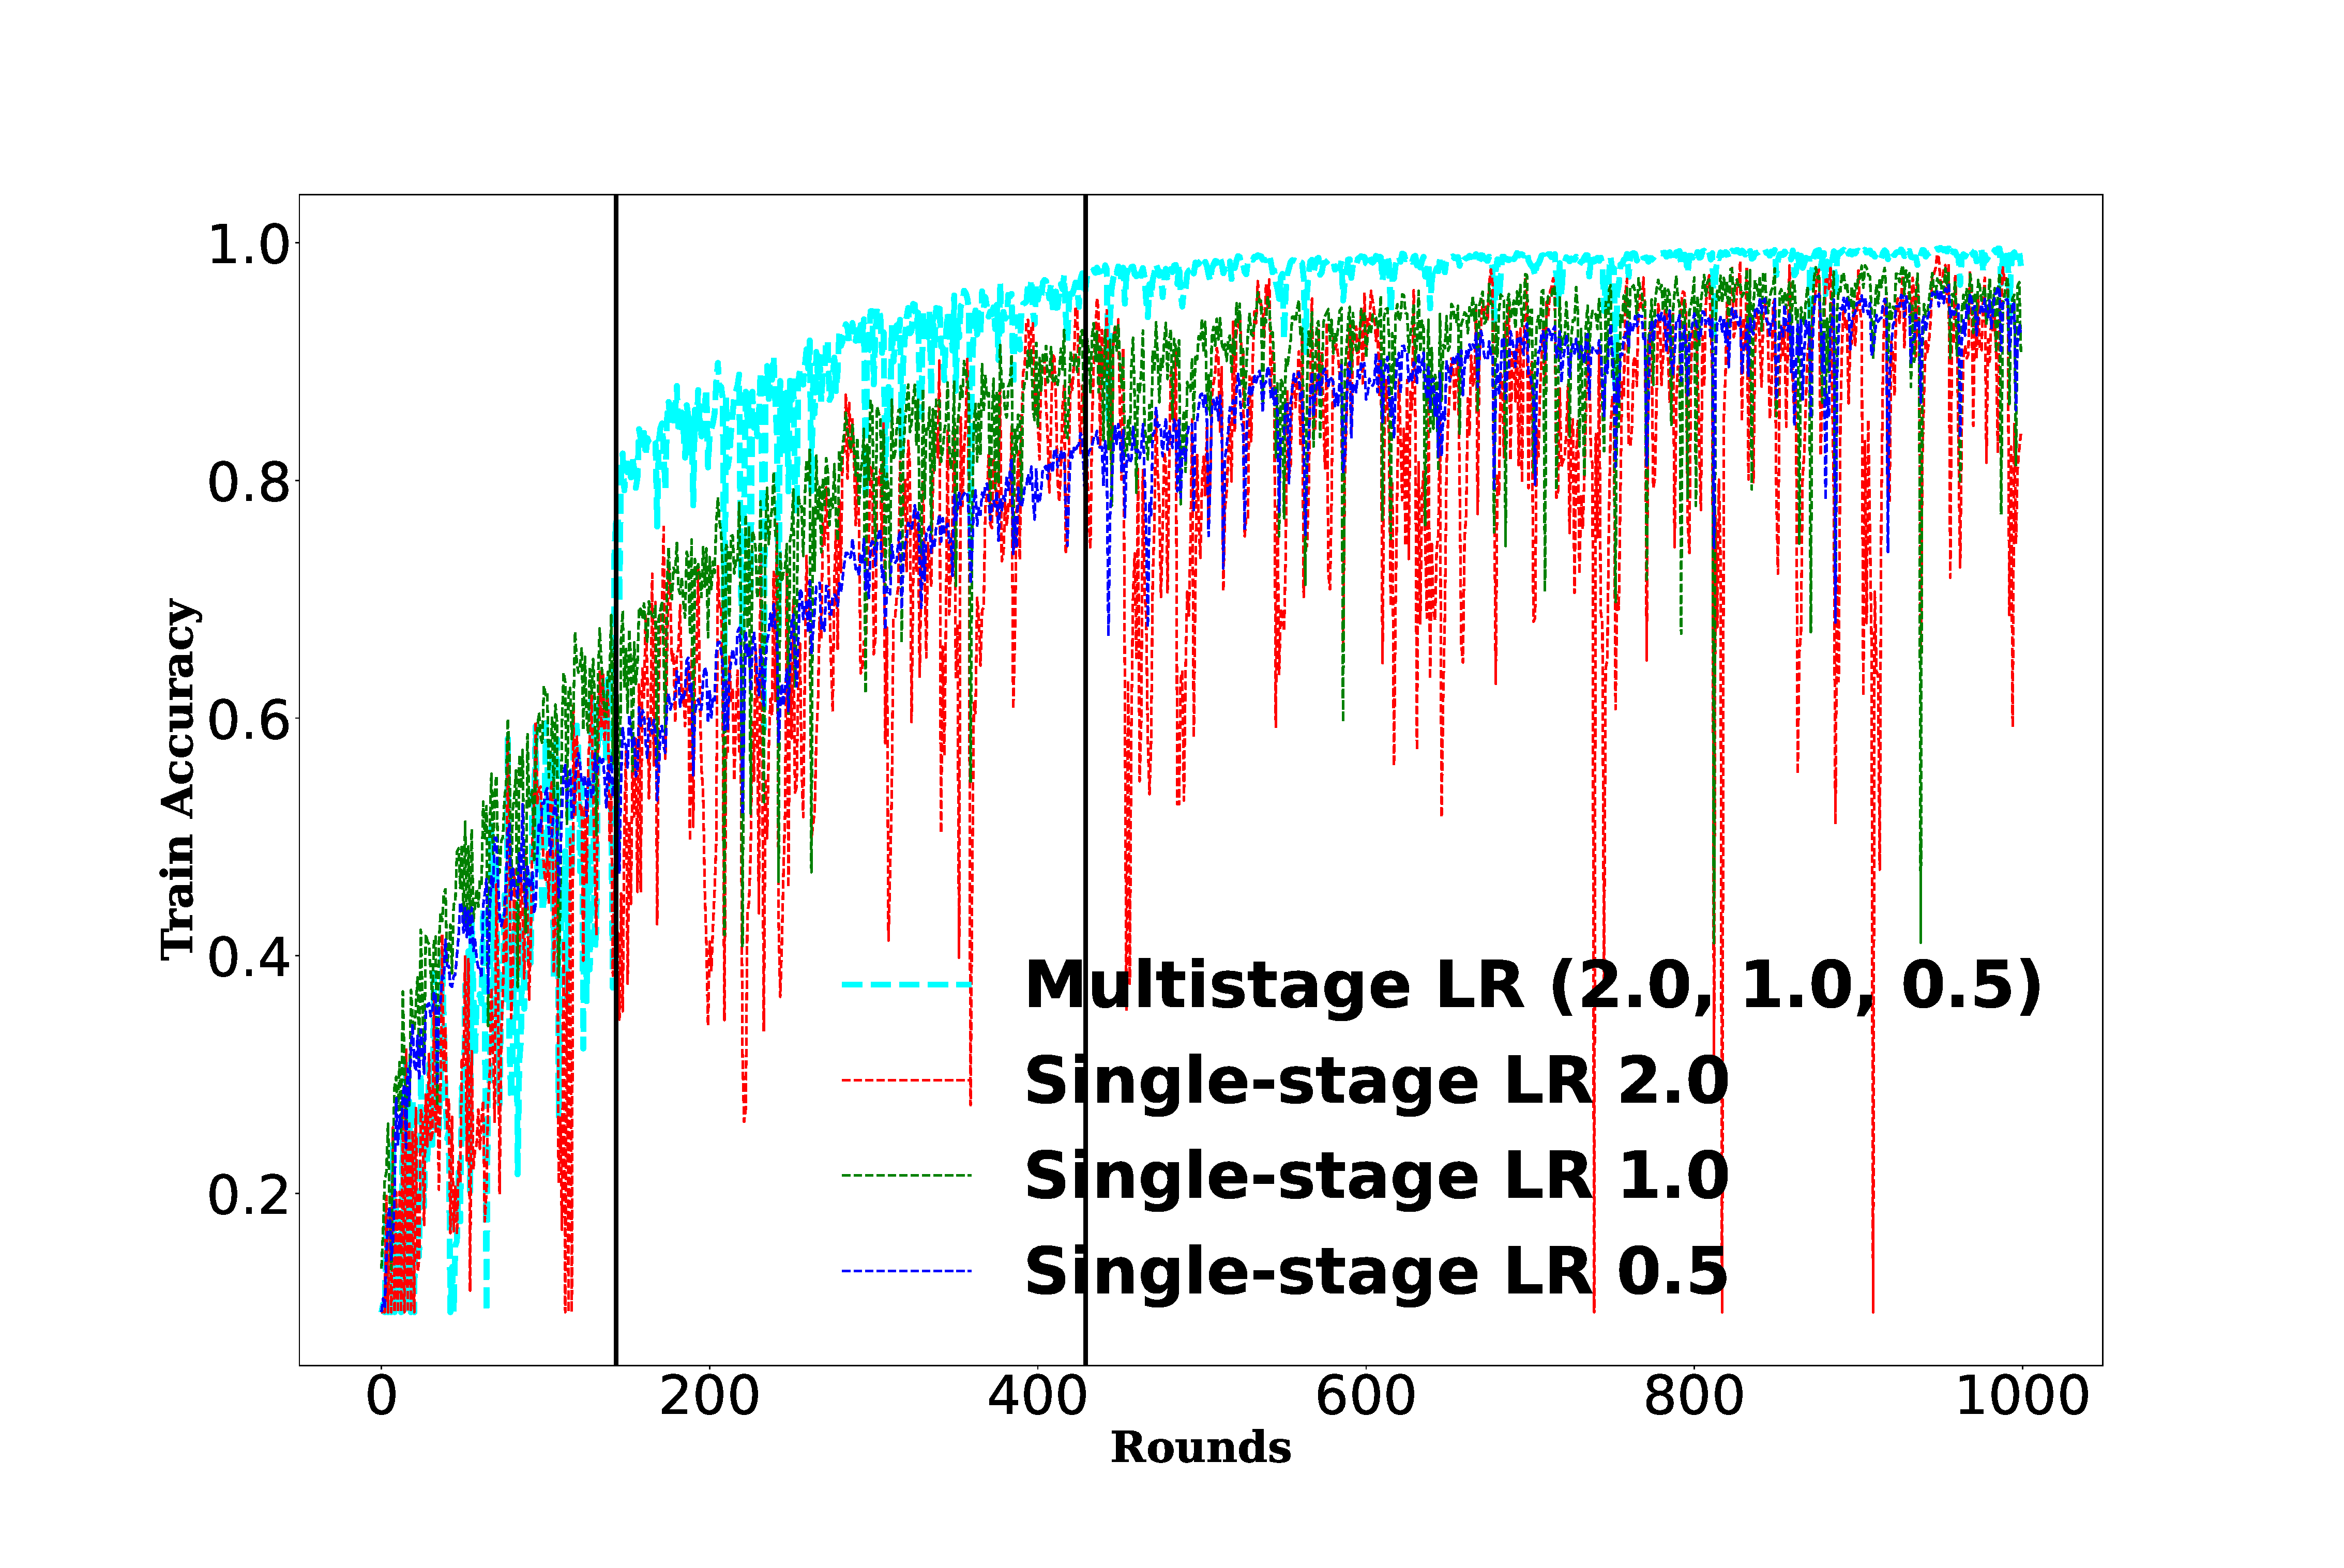
\includegraphics[width=.45\textwidth]{figs/multistage_train.eps}
\label{subfig:multistage_resnet_cifar10_train}
}
\subfigure{
\hspace{0pt}
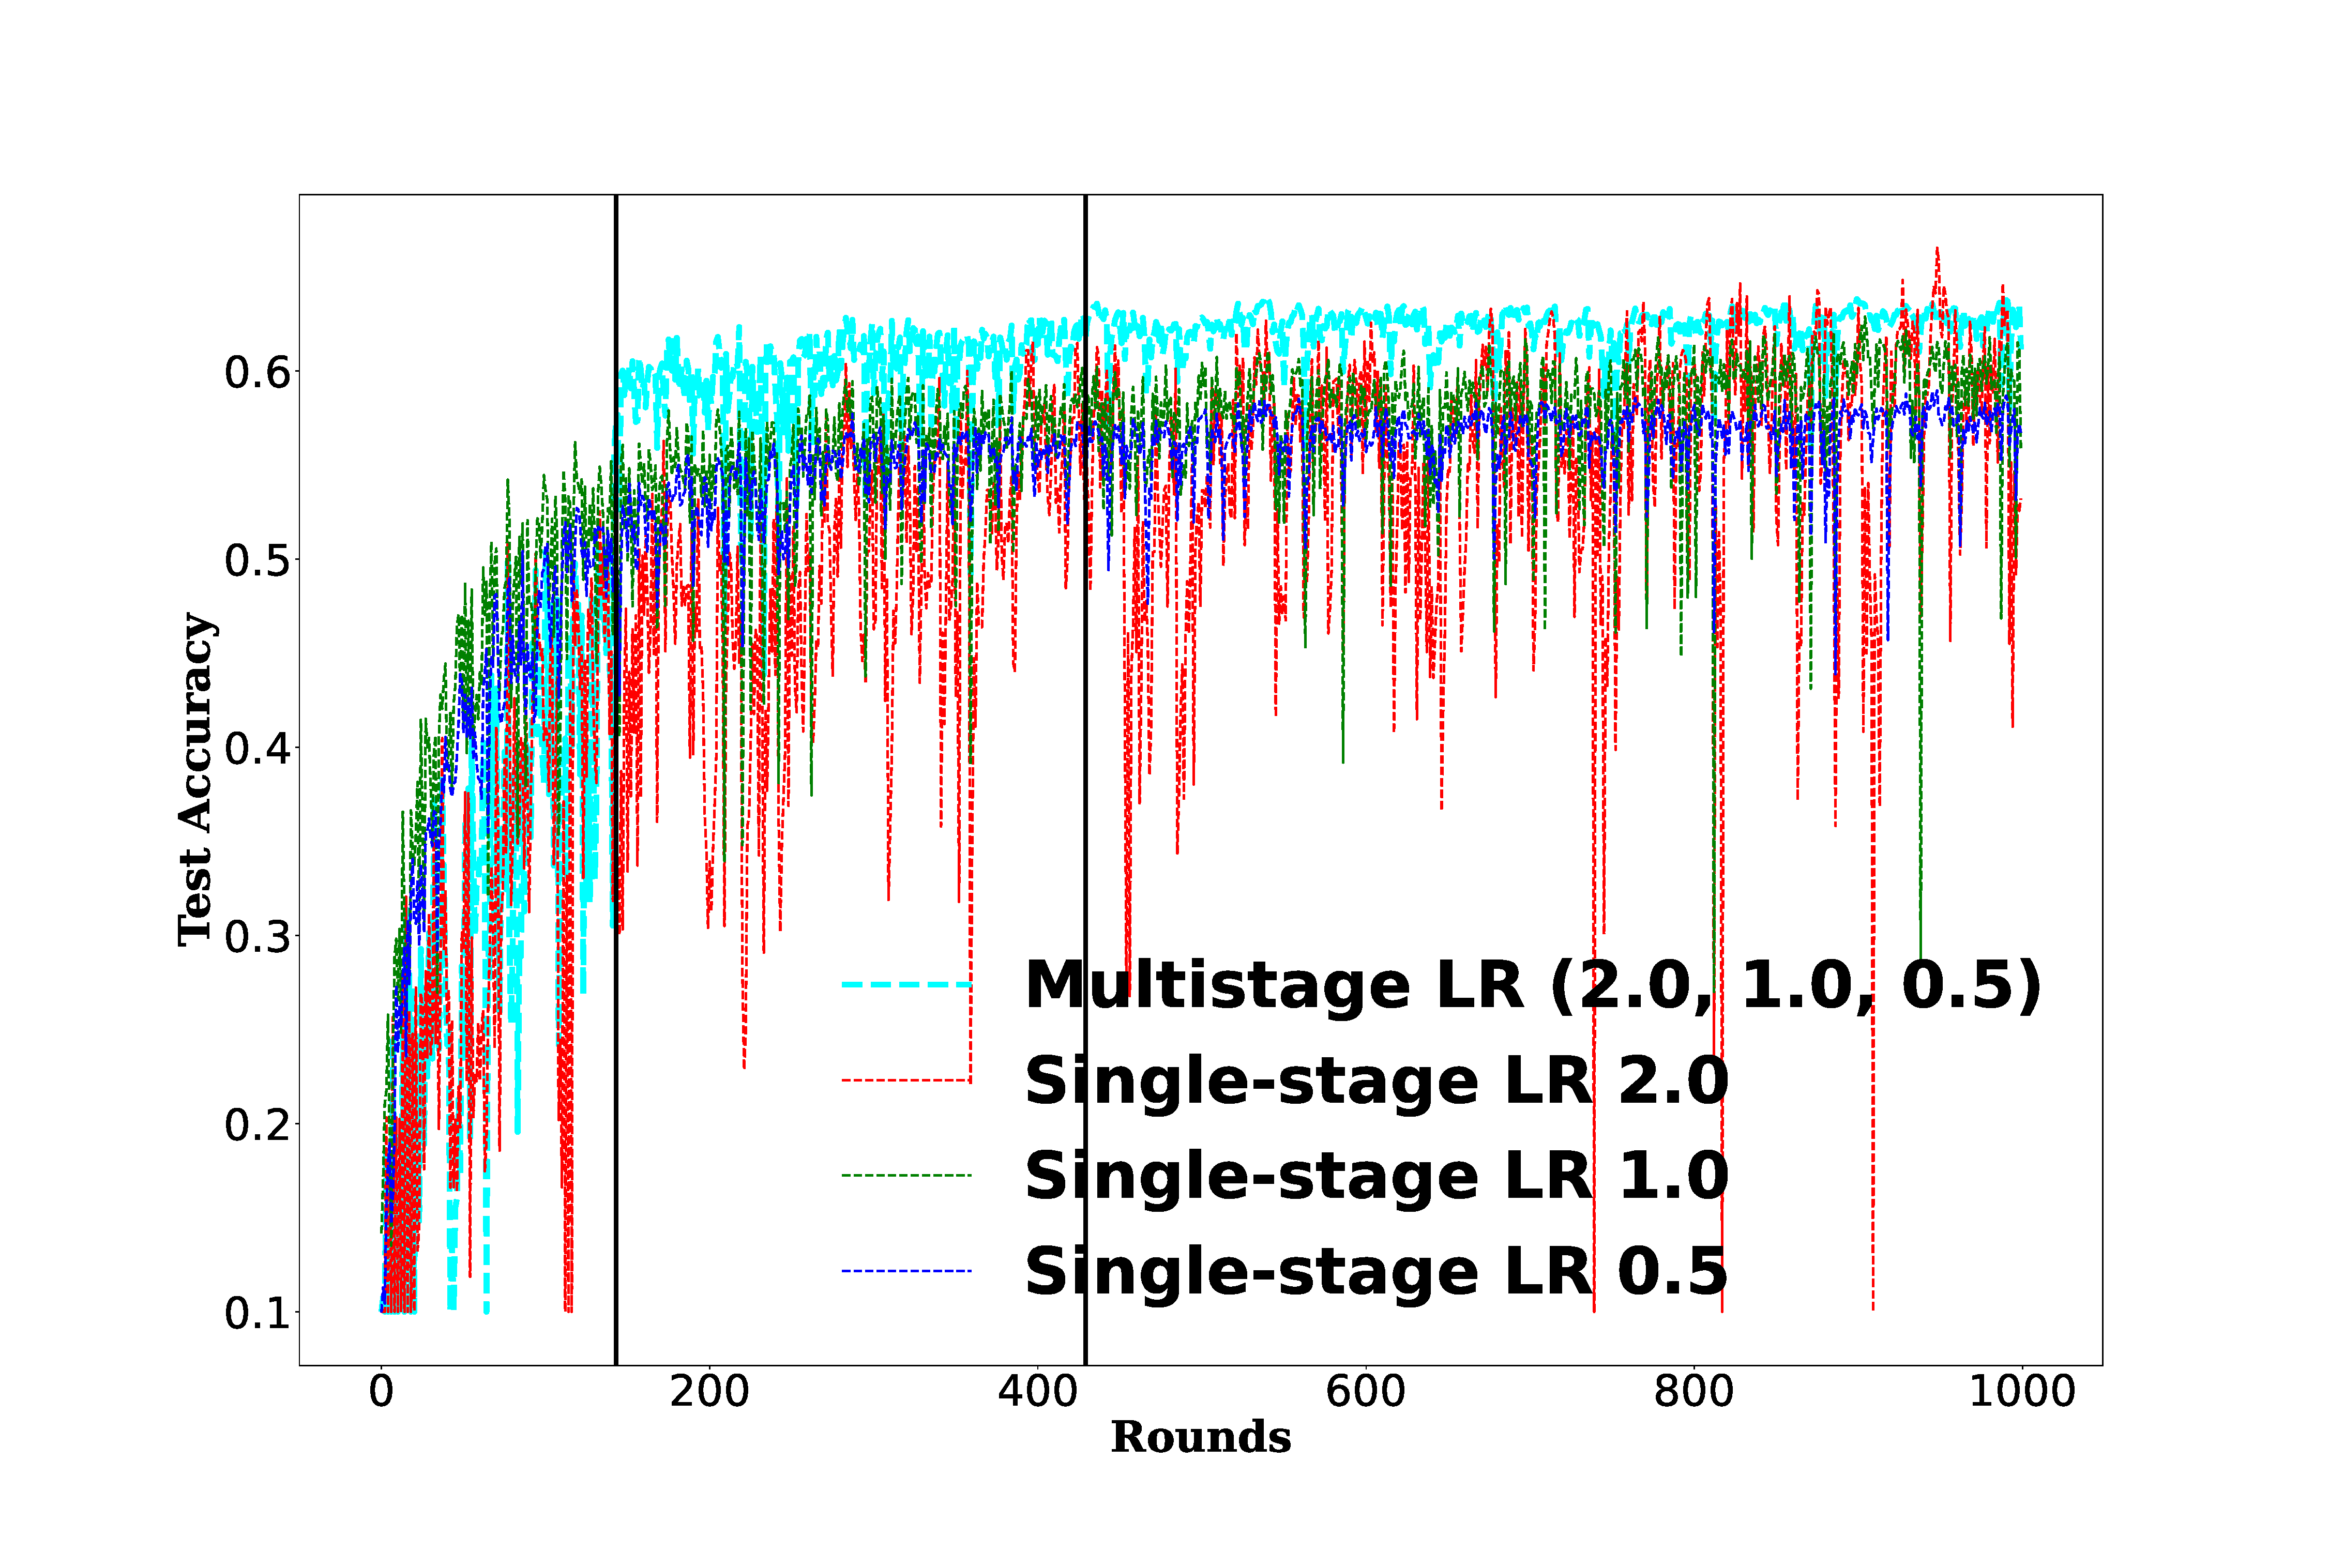
\includegraphics[width=.45\textwidth]{figs/multistage_test.eps}
\label{subfig:multistage_resnet_cifar10_test}
}
\vspace*{-6pt}
\caption{\ref{subfig:multistage_resnet_cifar10_train} Training and \ref{subfig:multistage_resnet_cifar10_test} Testing Curves for Multistage FedGM vs. Single-stage FedGM.}
\label{fig:resnet_cifar10_multistage_remake}
\end{figure}

\fi

Figure \ref{fig:2000r_multistage_resnet_cifar10} presents the results of running multistage FedGM for 2000 rounds, to see whether the advantage of multistage disappears with a longer training time. The two black vertical lines at round 286 and 857 mark the end of 1st/2nd stage. As we could observe from Figure \ref{fig:2000r_multistage_resnet_cifar10}, the superiority of multistage FedGM is consistent with longer training time.

\begin{figure}[h]
\vspace*{-6pt}
\centering
\subfigure{
\hspace{0pt}
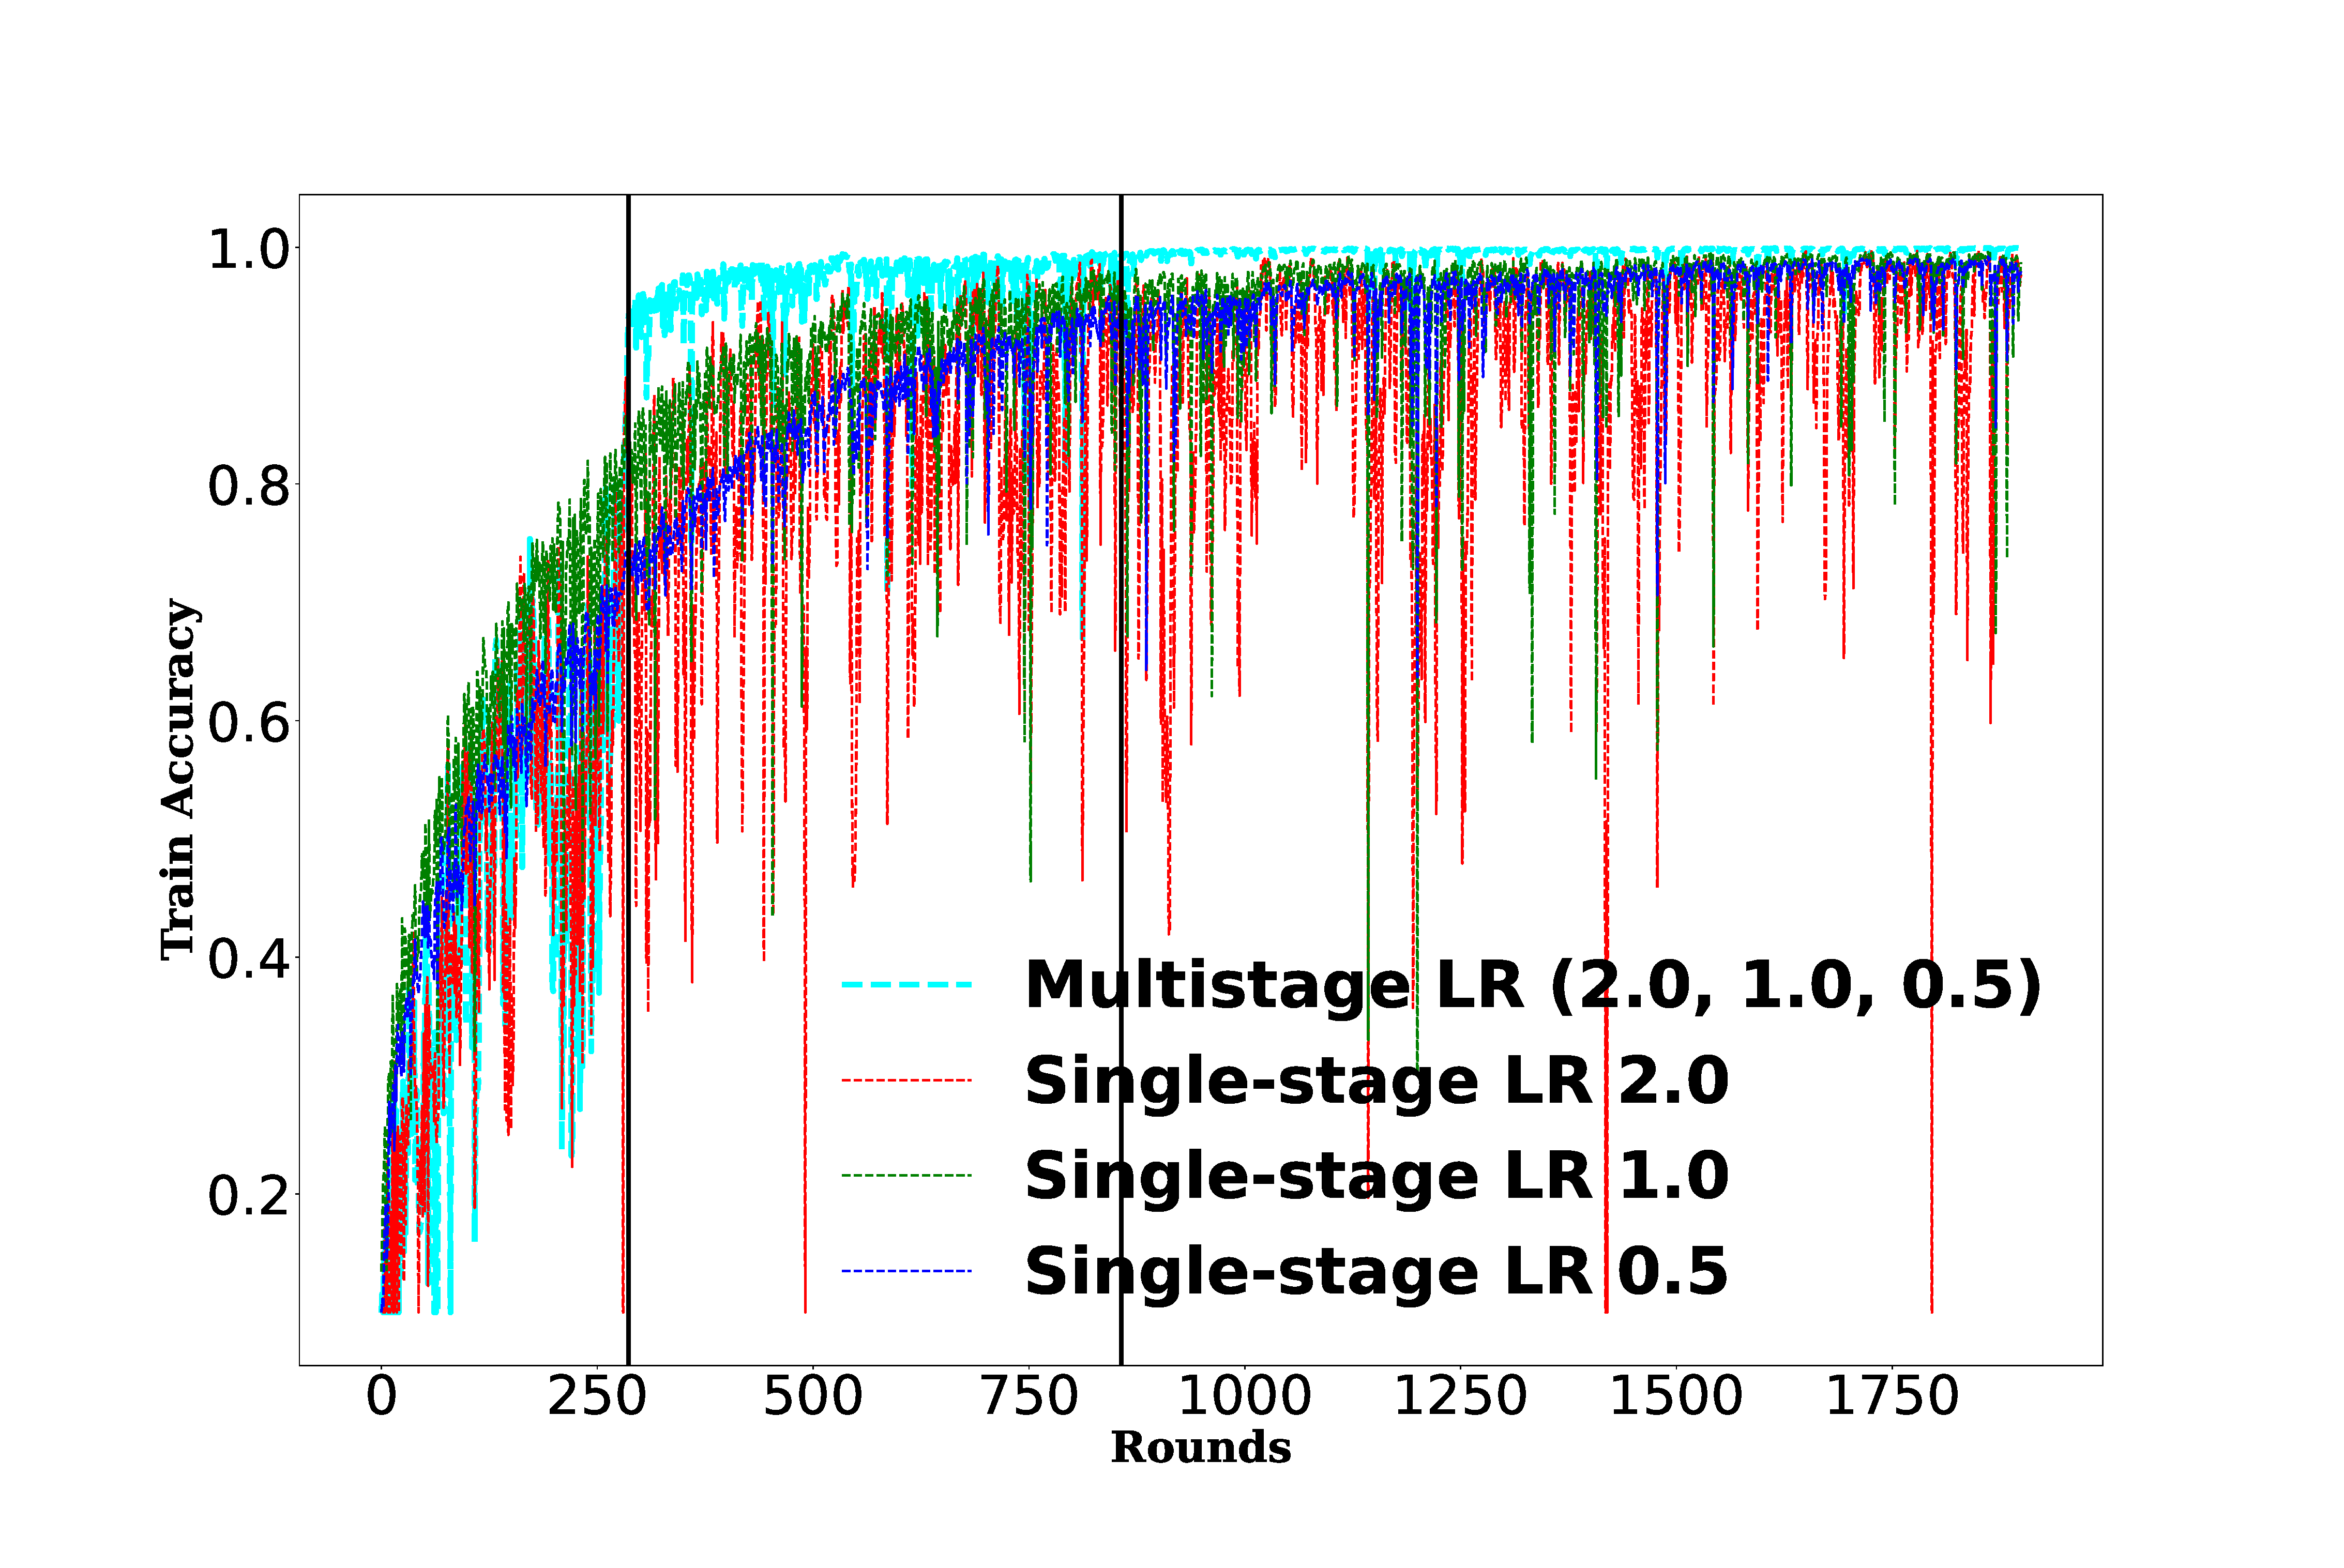
\includegraphics[width=.45\textwidth]{figs/2000r_multistage_train.eps}
\label{subfig:2000r_multistage_resnet_cifar10_train}
}
\subfigure{
\hspace{0pt}
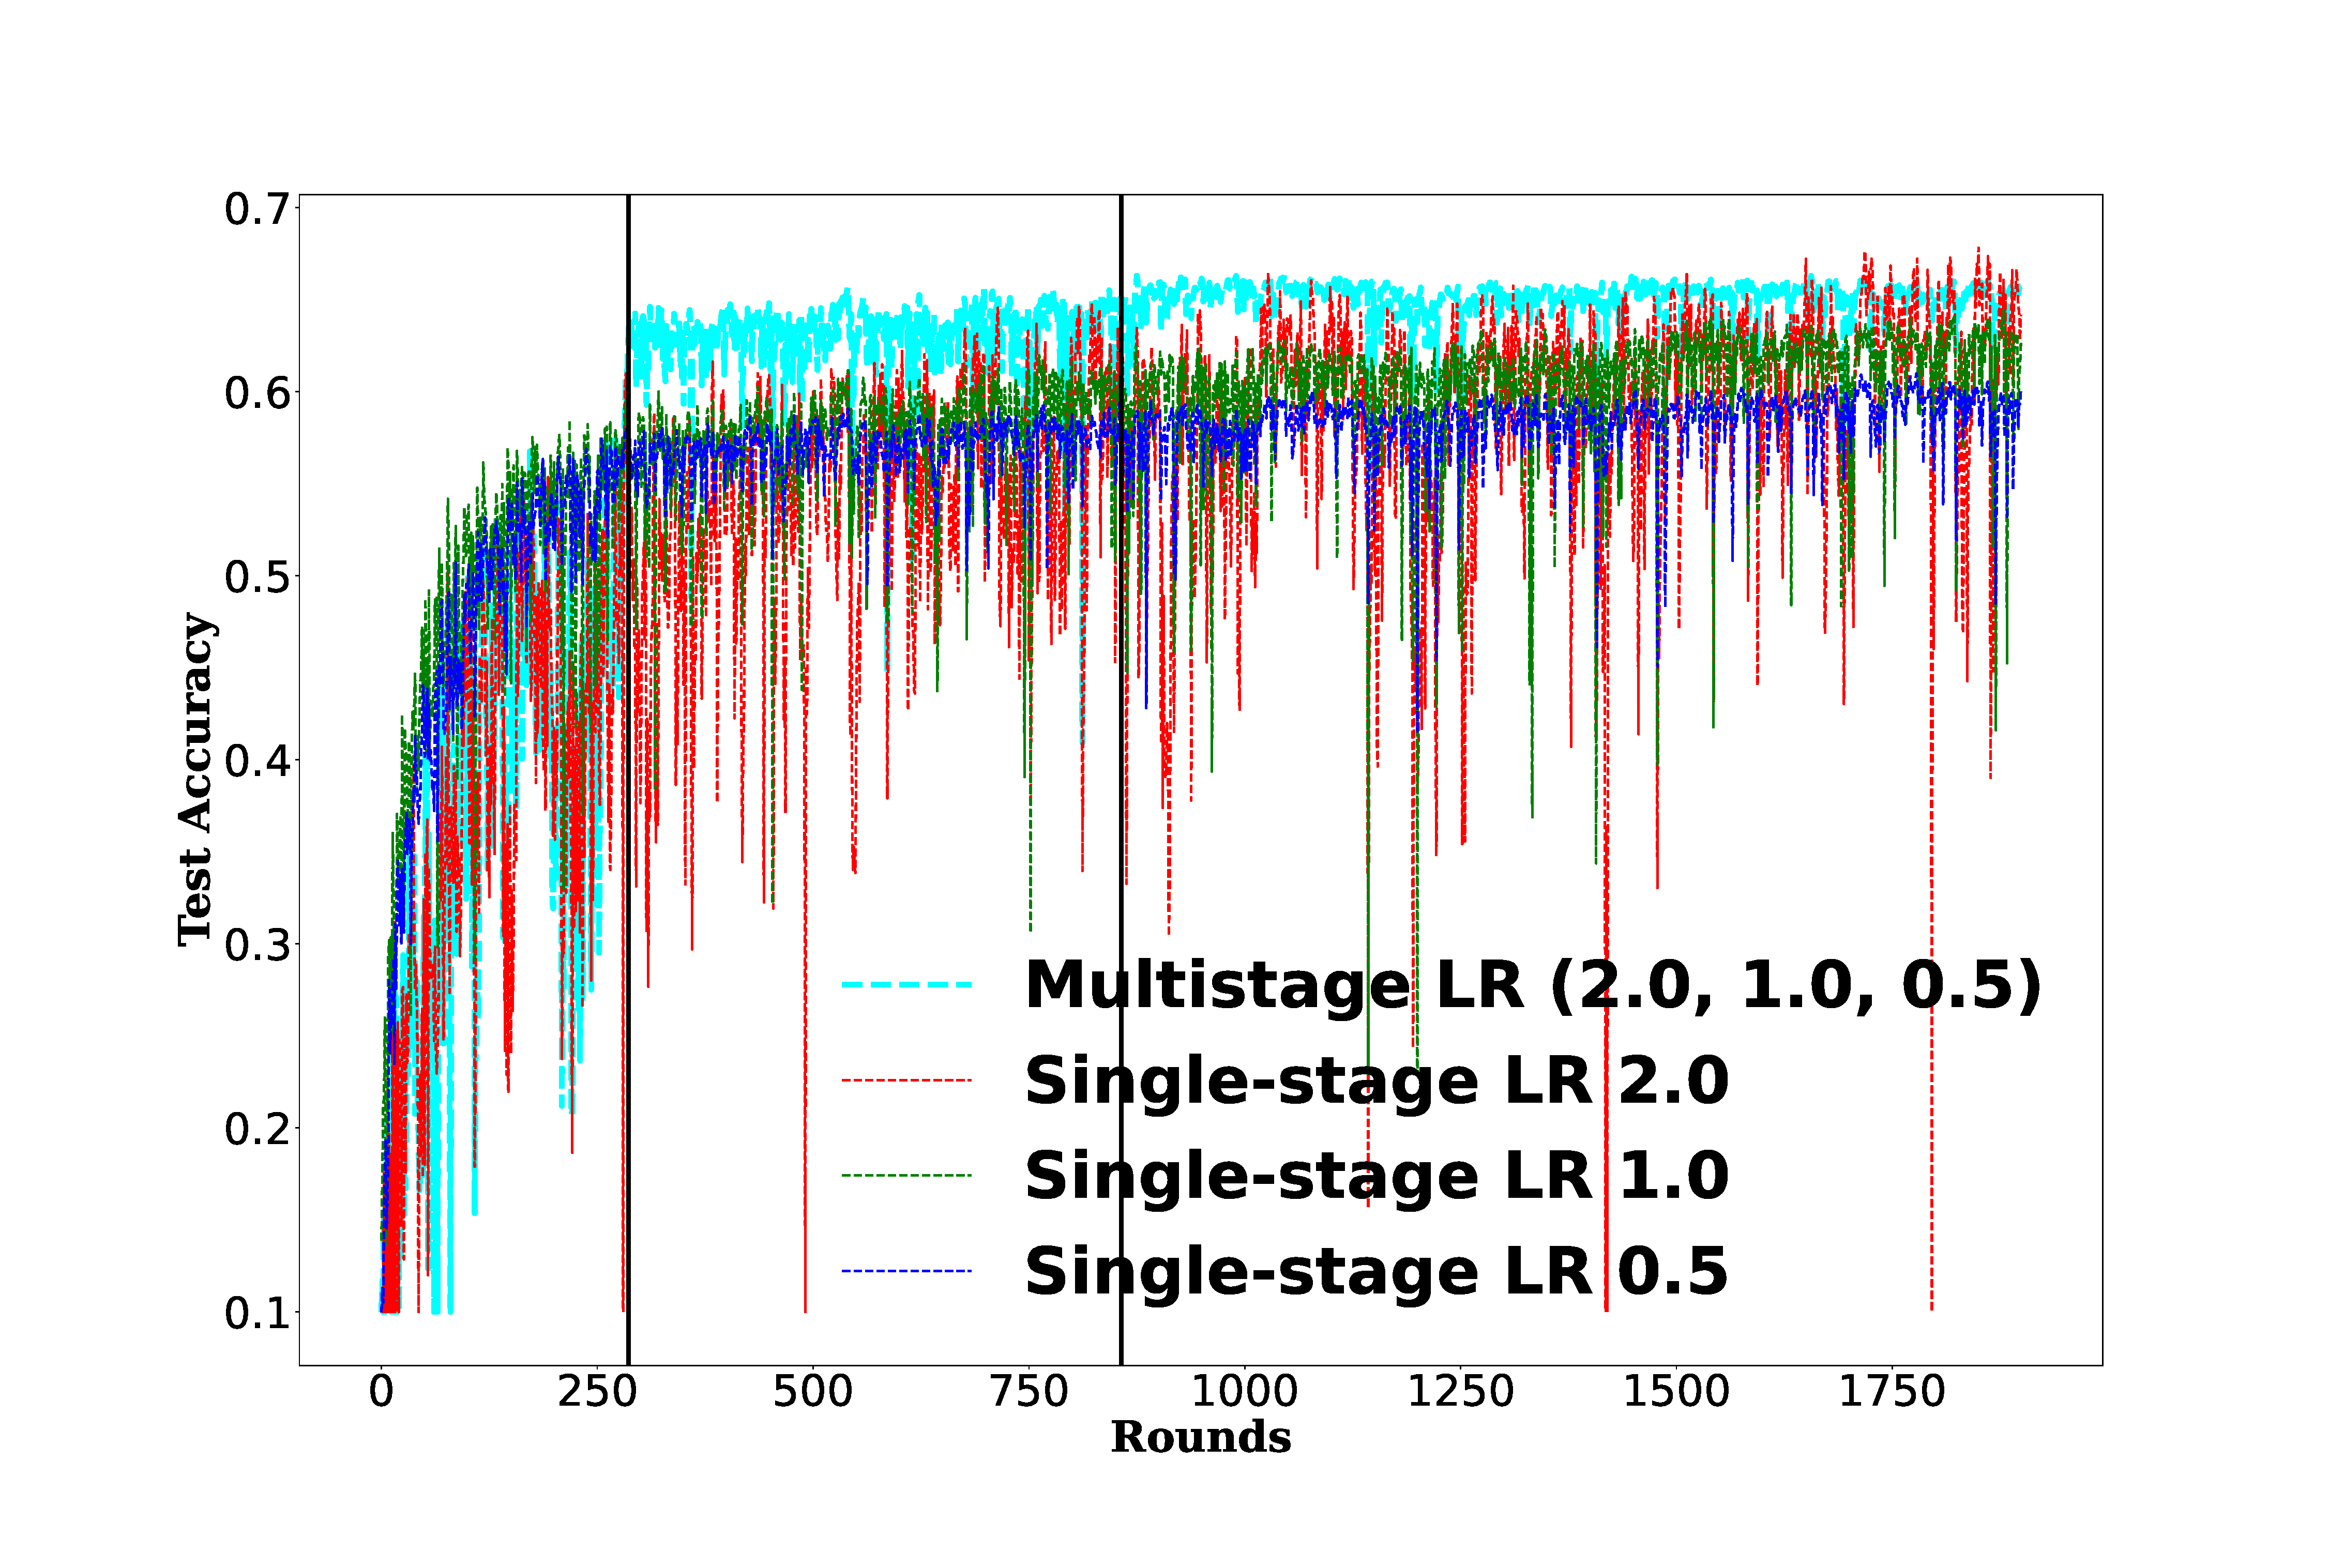
\includegraphics[width=.45\textwidth]{figs/2000r_multistage_test.eps}
\label{subfig:2000r_multistage_resnet_cifar10_test}
}
\vspace*{-6pt}
\caption{\ref{subfig:2000r_multistage_resnet_cifar10_train} Training and \ref{subfig:2000r_multistage_resnet_cifar10_test} Testing Curves for Multistage FedGM vs. Single-stage FedGM for 2000 rounds.}
\label{fig:2000r_multistage_resnet_cifar10}
\end{figure}

\subsection{More Experiments in Section \ref{subsec:exp_autonomous_fedgm}}
\label{subsec:appendix_more_exp_autonomous}

Figure \ref{fig:autonomous_varying_delay_result} shows the results for ResNet on CIFAR-10 with Autonomous FedGM and Autonomous FedAvg. The experimental settings are exactly same as Figure \ref{fig:resnet_cifar10} except the random delay is 10 instead of 5. Specifically, in  Figure \ref{fig:resnet_cifar10_autonomous} we allow each worker to select one global model randomly from the last recent 5 global models, while in Figure \ref{fig:resnet_cifar10} we allow each worker to select one global model randomly from the last recent 10 global models. The objective is to mimic different levels of asynchrony. We report the curves with best final test accuracy. We plot a FedGM (i.e. no random delay and identical local epochs) as a baseline. Similarly as Figure \ref{fig:resnet_cifar10}, we observe momentum is crucial as Autonomous FedGM outperforms Autonomous FedAvg with system heterogeneity. Autonomous FedGM does experience a slowdown compared to the ideal FedGM, but the difference is within a manageable margin, which validates the effectiveness of our proposed Autonomous FedGM.

\begin{figure}[h]
\vspace*{-12pt}
\centering
\subfigure{
\hspace{0pt}
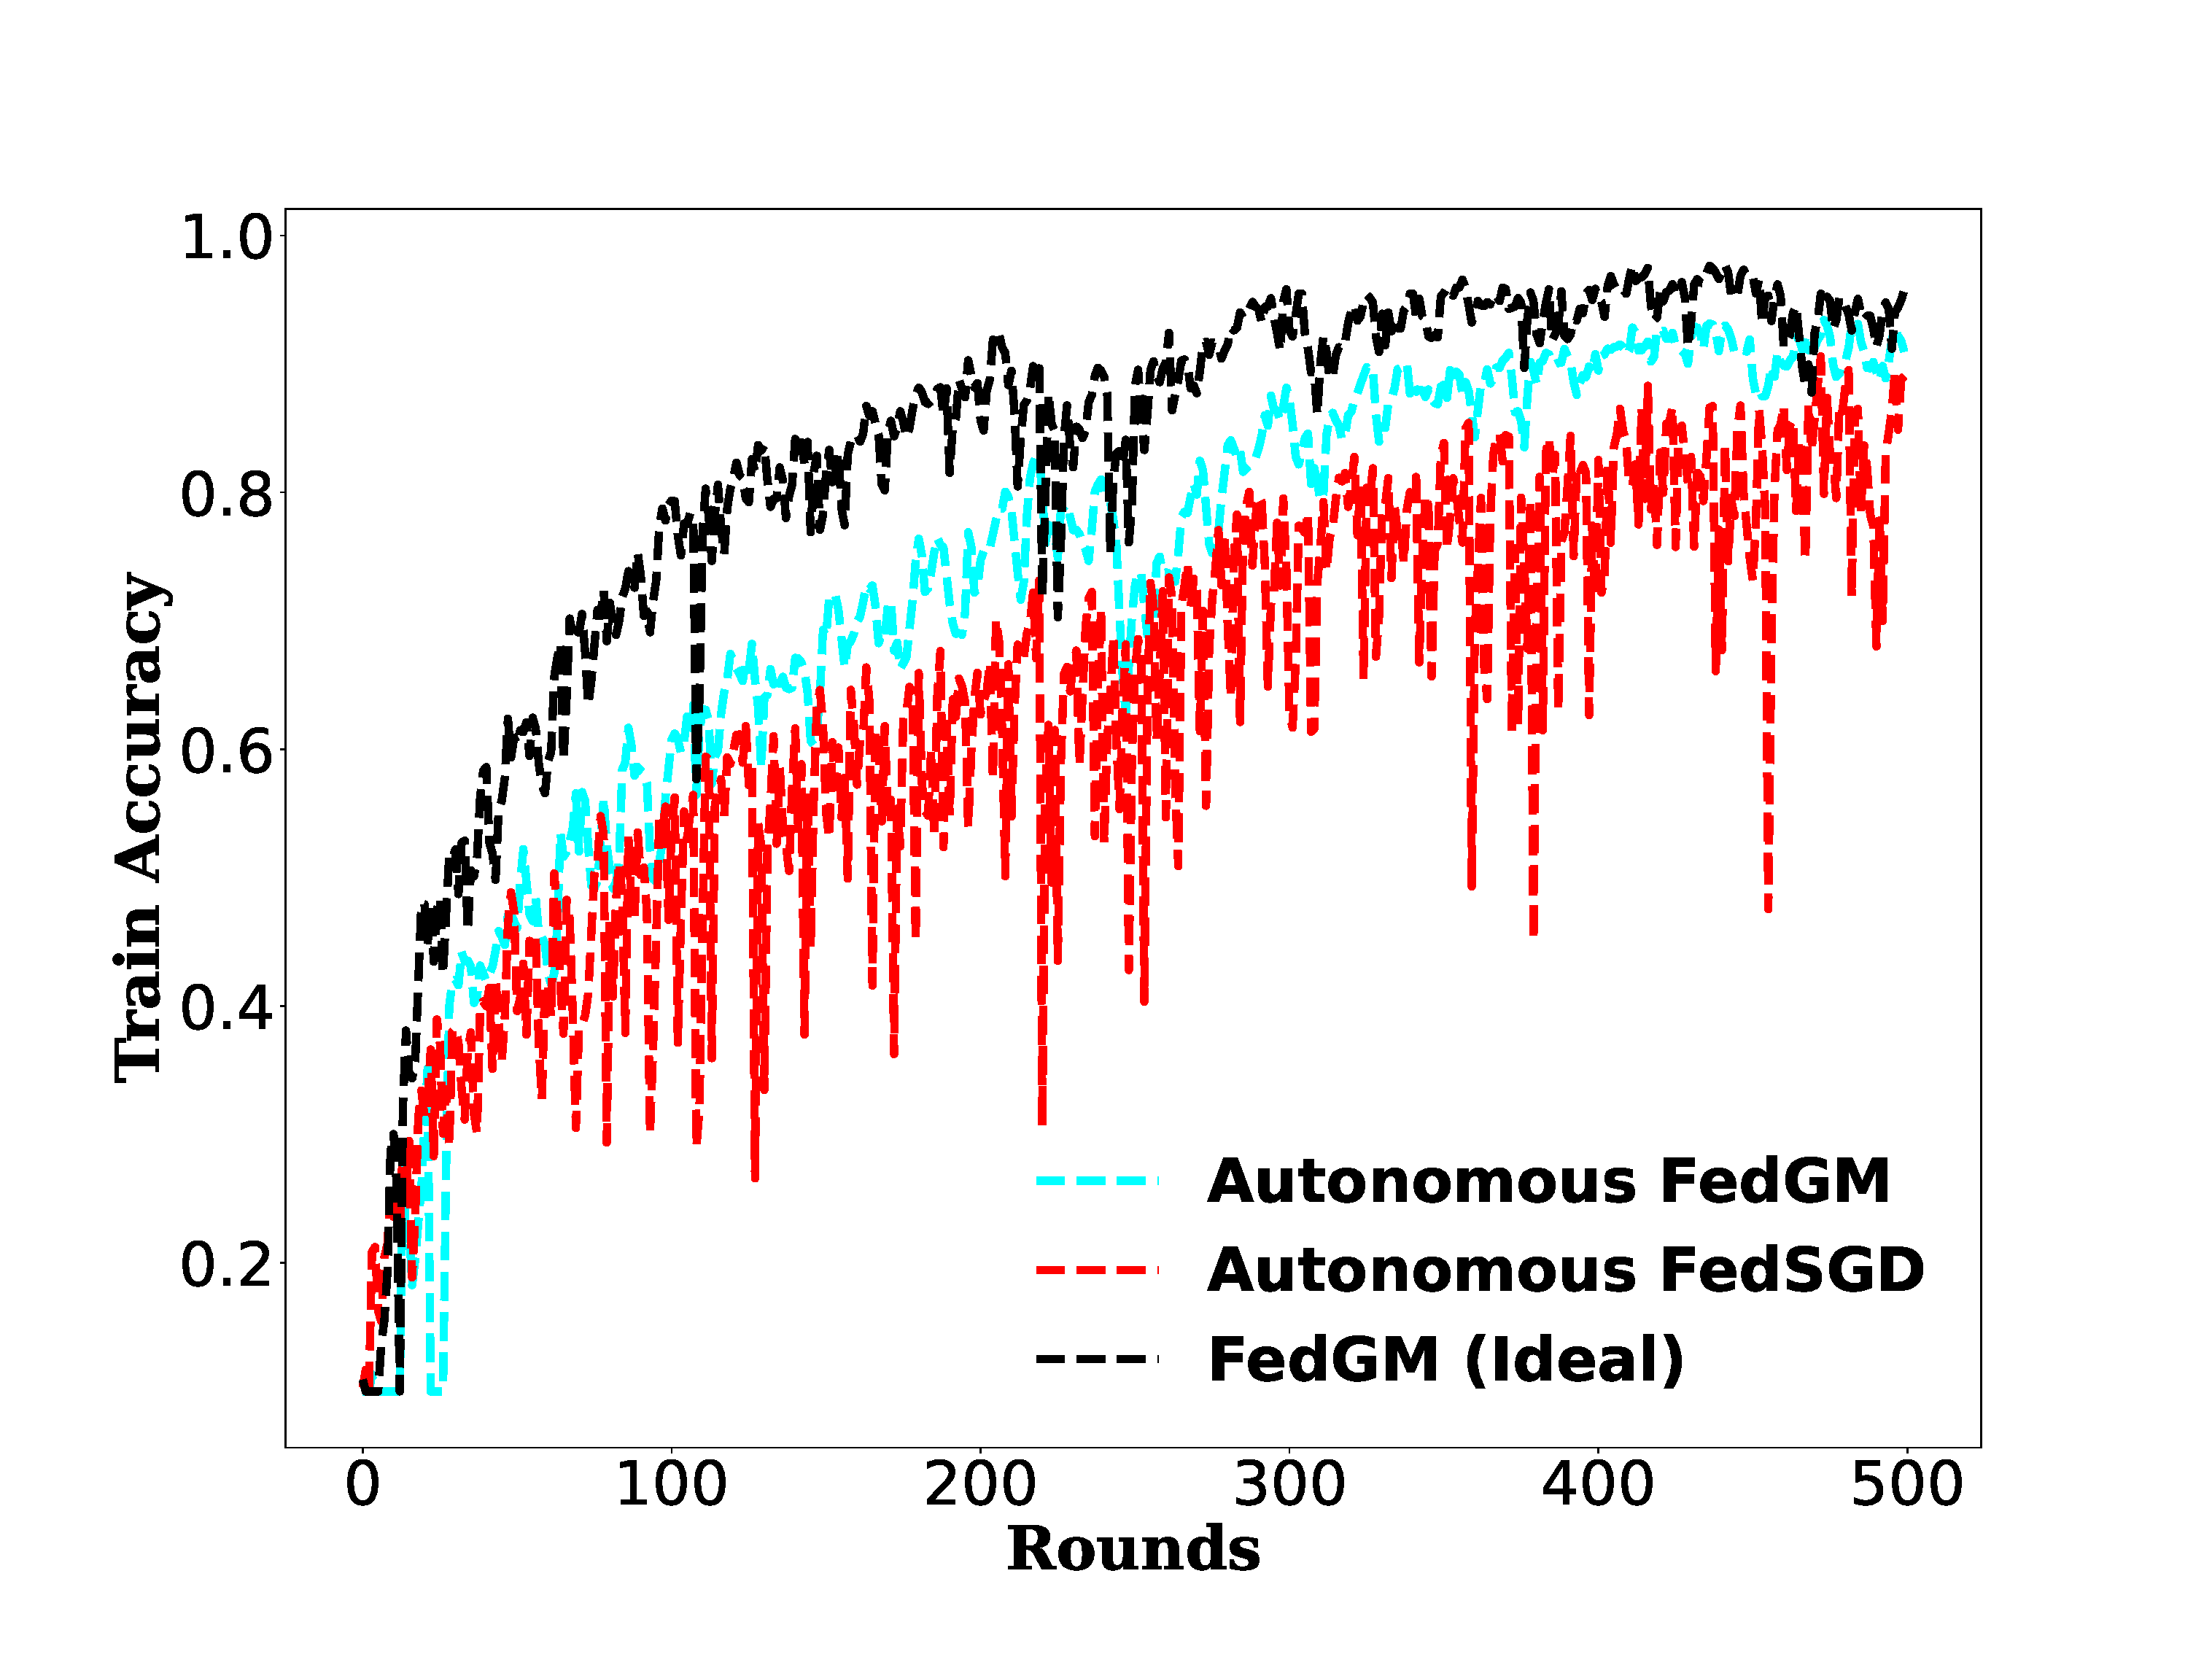
\includegraphics[width=.35\textwidth]{figs/autonomous_varying_delay_train.eps}
\label{subfig:autonomous_varying_delay_train}
}
\subfigure{
\hspace{0pt}
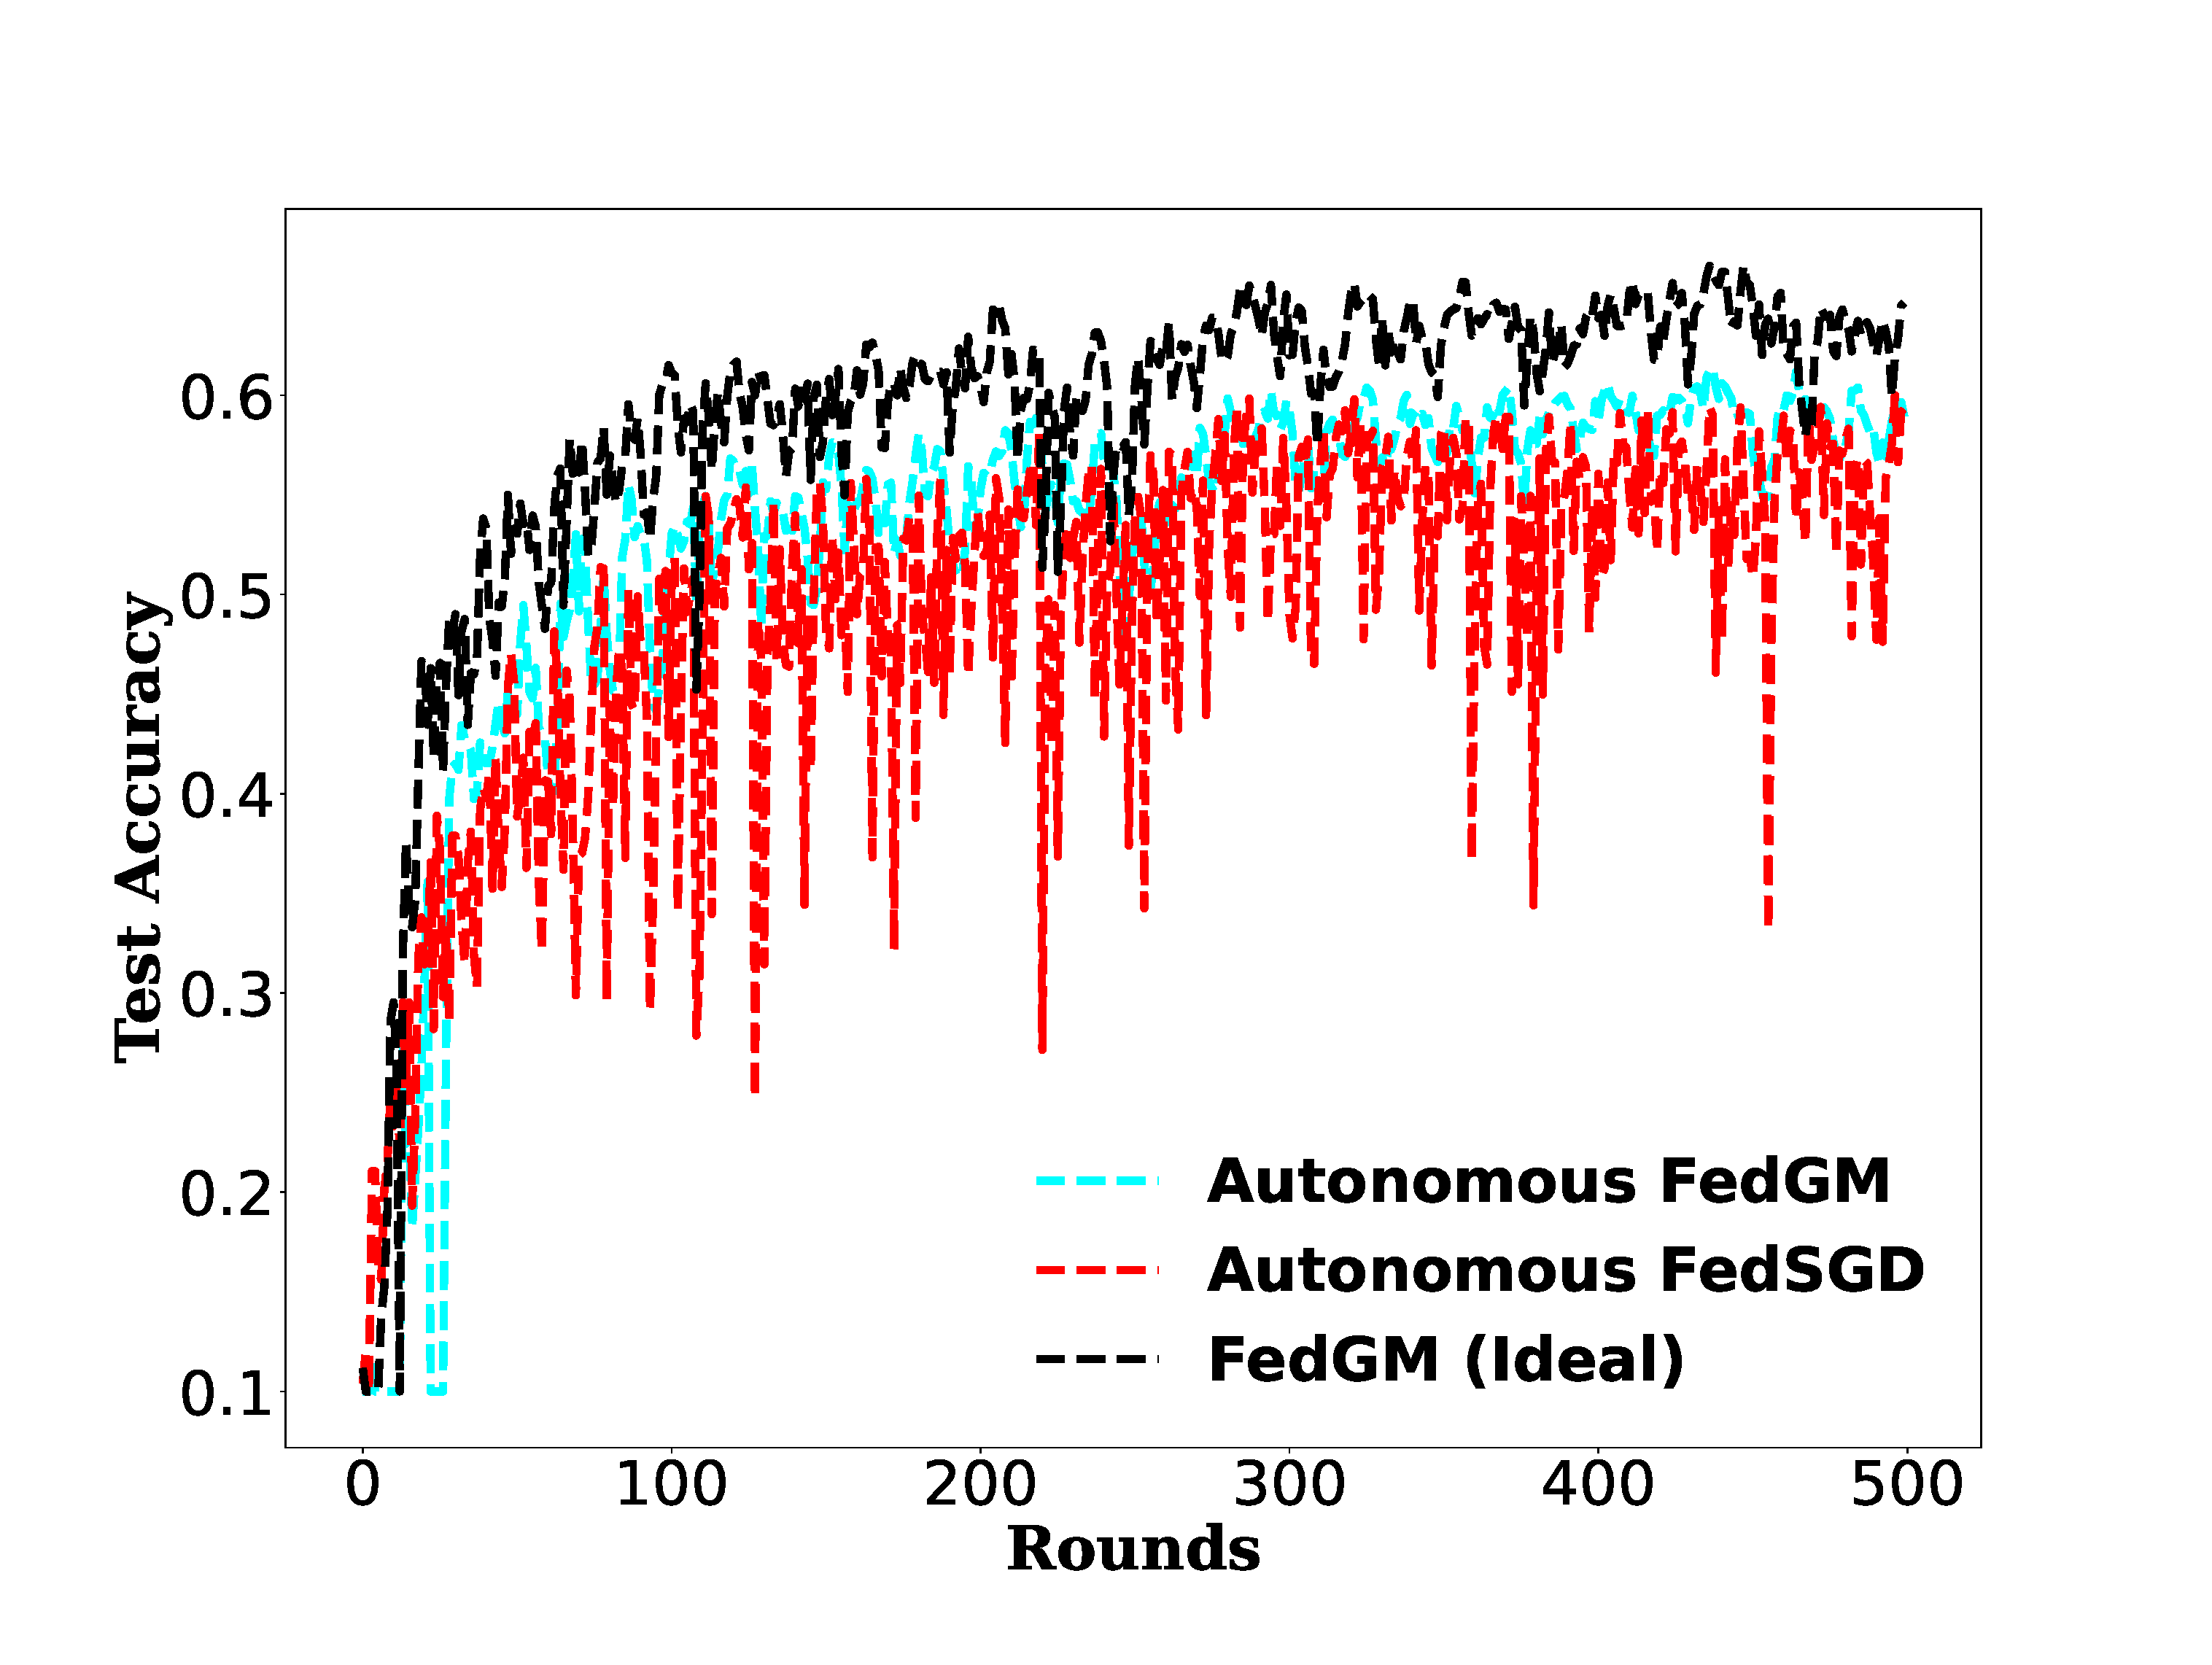
\includegraphics[width=.35\textwidth]{figs/autonomous_varying_delay_test.eps}
\label{subfig:autonomous_varying_delay_test}
}
\vspace*{-6pt}
\caption{\ref{subfig:autonomous_varying_delay_train} Training and \ref{subfig:autonomous_varying_delay_test} Testing Curve for ResNet on CIFAR-10 with Random Delay = 10.}
\label{fig:autonomous_varying_delay_result}
\end{figure}

\end{document}
